\newif\ifplotsrender
\plotsrendertrue
\documentclass{article}
\usepackage{ifluatex}
\ifluatex 
    \usepackage{fontspec}
    \setsansfont{CMU Sans Serif}%{Arial}
    \setmainfont{CMU Serif}%{Times New Roman}
    \setmonofont{CMU Typewriter Text}%{Consolas}
    \defaultfontfeatures{Ligatures={TeX}}
\else
    \usepackage[T2A]{fontenc}
    \usepackage[utf8]{inputenc}
\fi
\usepackage[english,russian]{babel}
\usepackage{amssymb,latexsym,amsmath,amscd,mathtools,wasysym}
\usepackage[shortlabels]{enumitem}
\usepackage[makeroom]{cancel}
\usepackage{graphicx}
\usepackage{geometry}
\usepackage{verbatim}
\usepackage{fvextra}

\usepackage{longtable}
\usepackage{multirow}
\usepackage{multicol}
\usepackage{tabu}
\usepackage{arydshln} % \hdashline and :

\usepackage{float}
\makeatletter
\g@addto@macro\@floatboxreset\centering
\makeatother
\usepackage{caption}
\usepackage{csquotes}
\usepackage[bb=dsserif]{mathalpha}
\usepackage[normalem]{ulem}

\usepackage[e]{esvect}
\let\vec\vv

\usepackage{xcolor}
\colorlet{darkgreen}{black!25!blue!50!green}


%% Here f*cking with mathabx
\DeclareFontFamily{U}{matha}{\hyphenchar\font45}
\DeclareFontShape{U}{matha}{m}{n}{
    <5> <6> <7> <8> <9> <10> gen * matha
    <10.95> matha10 <12> <14.4> <17.28> <20.74> <24.88> matha12
}{}
\DeclareSymbolFont{matha}{U}{matha}{m}{n}
\DeclareFontFamily{U}{mathb}{\hyphenchar\font45}
\DeclareFontShape{U}{mathb}{m}{n}{
    <5> <6> <7> <8> <9> <10> gen * mathb
    <10.95> matha10 <12> <14.4> <17.28> <20.74> <24.88> mathb12
}{}
\DeclareSymbolFont{mathb}{U}{mathb}{m}{n}

\DeclareMathSymbol{\defeq}{\mathrel}{mathb}{"15}
\DeclareMathSymbol{\eqdef}{\mathrel}{mathb}{"16}


\usepackage{trimclip}
\DeclareMathOperator{\updownarrows}{\clipbox{0pt 0pt 4.175pt 0pt}{$\upuparrows$}\hspace{-.825px}\clipbox{0pt 0pt 4.175pt 0pt}{$\downdownarrows$}}
\DeclareMathOperator{\downuparrows}{\clipbox{0pt 0pt 4.175pt 0pt}{$\downdownarrows$}\hspace{-.825px}\clipbox{0pt 0pt 4.175pt 0pt}{$\upuparrows$}}

\makeatletter
\providecommand*\deletecounter[1]{%
    \expandafter\let\csname c@#1\endcsname\@undefined}
\makeatother


\usepackage{hyperref}
\hypersetup{
    %hidelinks,
    colorlinks=true,
    linkcolor=darkgreen,
    urlcolor=blue,
    breaklinks=true,
}

\usepackage{pgf}
\usepackage{pgfplots}
\pgfplotsset{compat=newest}
\usepackage{tikz,tikz-3dplot}
\usepackage{tkz-euclide}
\usetikzlibrary{calc,automata,patterns,angles,quotes,backgrounds,shapes.geometric,trees,positioning,decorations.pathreplacing}
\pgfkeys{/pgf/plot/gnuplot call={T: && cd TeX && gnuplot}}
\usepgfplotslibrary{fillbetween,polar}
\ifluatex
\usetikzlibrary{graphs,graphs.standard,graphdrawing,quotes,babel}
\usegdlibrary{layered,trees,circular,force}
\else
\errmessage{Run with LuaTeX, if you want to use gdlibraries}
\fi
\makeatletter
\newcommand\currentnode{\the\tikz@lastxsaved,\the\tikz@lastysaved}
\makeatother

%\usepgfplotslibrary{external} 
%\tikzexternalize

\makeatletter
\newcommand*\circled[2][1.0]{\tikz[baseline=(char.base)]{
        \node[shape=circle, draw, inner sep=2pt,
        minimum height={\f@size*#1},] (char) {#2};}}
\makeatother

\newcommand{\existence}{{\circled{$\exists$}}}
\newcommand{\uniqueness}{{\circled{$\hspace{0.5px}!$}}}
\newcommand{\rightimp}{{\circled{$\Rightarrow$}}}
\newcommand{\leftimp}{{\circled{$\Leftarrow$}}}

\DeclareMathOperator{\sign}{sign}
\DeclareMathOperator{\Cl}{Cl}
\DeclareMathOperator{\proj}{pr}
\DeclareMathOperator{\Arg}{Arg}
\DeclareMathOperator{\supp}{supp}
\DeclareMathOperator{\diag}{diag}
\DeclareMathOperator{\tr}{tr}
\DeclareMathOperator{\rank}{rank}
\DeclareMathOperator{\Lat}{Lat}
\DeclareMathOperator{\Lin}{Lin}
\DeclareMathOperator{\Ln}{Ln}
\DeclareMathOperator{\Orbit}{Orbit}
\DeclareMathOperator{\St}{St}
\DeclareMathOperator{\Seq}{Seq}
\DeclareMathOperator{\PSet}{PSet}
\DeclareMathOperator{\MSet}{MSet}
\DeclareMathOperator{\Cyc}{Cyc}
\DeclareMathOperator{\Hom}{Hom}
\DeclareMathOperator{\End}{End}
\DeclareMathOperator{\Aut}{Aut}
\DeclareMathOperator{\Ker}{Ker}
\DeclareMathOperator{\Def}{def}
\DeclareMathOperator{\Alt}{Alt}
\DeclareMathOperator{\Sim}{Sim}
\DeclareMathOperator{\Int}{Int}
\DeclareMathOperator{\grad}{grad}
\DeclareMathOperator{\sech}{sech}
\DeclareMathOperator{\csch}{csch}
\DeclareMathOperator{\asin}{\sin^{-1}}
\DeclareMathOperator{\acos}{\cos^{-1}}
\DeclareMathOperator{\atan}{\tan^{-1}}
\DeclareMathOperator{\acot}{\cot^{-1}}
\DeclareMathOperator{\asec}{\sec^{-1}}
\DeclareMathOperator{\acsc}{\csc^{-1}}
\DeclareMathOperator{\asinh}{\sinh^{-1}}
\DeclareMathOperator{\acosh}{\cosh^{-1}}
\DeclareMathOperator{\atanh}{\tanh^{-1}}
\DeclareMathOperator{\acoth}{\coth^{-1}}
\DeclareMathOperator{\asech}{\sech^{-1}}
\DeclareMathOperator{\acsch}{\csch^{-1}}

\newcommand*{\scriptA}{{\mathcal{A}}}
\newcommand*{\scriptB}{{\mathcal{B}}}
\newcommand*{\scriptC}{{\mathcal{C}}}
\newcommand*{\scriptD}{{\mathcal{D}}}
\newcommand*{\scriptF}{{\mathcal{F}}}
\newcommand*{\scriptH}{{\mathcal{H}}}
\newcommand*{\scriptK}{{\mathcal{K}}}
\newcommand*{\scriptL}{{\mathcal{L}}}
\newcommand*{\scriptM}{{\mathcal{M}}}
\newcommand*{\scriptP}{{\mathcal{P}}}
\newcommand*{\scriptQ}{{\mathcal{Q}}}
\newcommand*{\scriptR}{{\mathcal{R}}}
\newcommand*{\scriptT}{{\mathcal{T}}}
\newcommand*{\scriptU}{{\mathcal{U}}}
\newcommand*{\scriptX}{{\mathcal{X}}}
\newcommand*{\Cnk}[2]{\left(\begin{matrix}#1\\#2\end{matrix}\right)}
\newcommand*{\im}{{\mathbf i}}
\newcommand*{\id}{{\mathrm{id}}}
\newcommand*{\compl}{^\complement}
\newcommand*{\dotprod}[2]{{\left\langle{#1},{#2}\right\rangle}}
\newcommand\matr[1]{\left(\begin{matrix}#1\end{matrix}\right)}
\newcommand\matrd[1]{\left|\begin{matrix}#1\end{matrix}\right|}
\newcommand\arr[2]{\left(\begin{array}{#1}#2\end{array}\right)}

\DeclareMathOperator{\divby}{\scalebox{1}[.65]{\vdots}}
\DeclareMathOperator{\toto}{\rightrightarrows}
\DeclareMathOperator{\ntoto}{\not\rightrightarrows}

\newcommand{\undercolorblack}[2]{{\color{#1}\underline{\color{black}#2}}}
\newcommand{\undercolor}[2]{{\colorlet{tmp}{.}\color{#1}\underline{\color{tmp}#2}}}

\usepackage{adjustbox}

\geometry{margin=1in}
\usepackage{fancyhdr}
\pagestyle{fancy}
\fancyfoot[L]{}
\fancyfoot[C]{Иванов Тимофей}
\fancyfoot[R]{\pagename\ \thepage}
\fancyhead[L]{}
\fancyhead[R]{\leftmark}
\renewcommand{\sectionmark}[1]{\markboth{#1}{}}

\setcounter{tocdepth}{5}
\newcommand{\dfn}{\item[\color{red}\textbullet]}
\newcommand{\thm}{\item[\color{darkgreen}\textbullet]}

\usepackage[framemethod=TikZ]{mdframed}
\mdfdefinestyle{MyFrame}{
    %linecolor=green!50!red!50!blue, %here we have 50% of blue and 25% of green and red.
    outerlinewidth=1pt,
    roundcorner=0px,
    innertopmargin=\baselineskip,
    innerbottommargin=\baselineskip,
    innerleftmargin=\baselineskip,
    innerrightmargin=\baselineskip}
\mdfdefinestyle{Proof}{
    style=MyFrame,
    fontcolor=black,
    linecolor=darkgreen,
    backgroundcolor=black!10!white,
}
\mdfdefinestyle{Example}{
    style=MyFrame,
    linecolor=yellow,
    fontcolor=black,
    backgroundcolor=black!10!white,
}
\mdfdefinestyle{Comment}{
    style=MyFrame,
    linecolor=black,
    backgroundcolor=black,
    fontcolor=white,
    roundcorner=10px,
}

\newenvironment{Proof}{\begin{mdframed}[style=Proof]}{\end{mdframed}}
\newenvironment{Example}{\begin{mdframed}[style=Example]}{\end{mdframed}}
\newenvironment{Comment}{\begin{mdframed}[style=Comment]}{\end{mdframed}}


\usepackage[e]{esvect}
\let\vec\vv

% \usepackage[e]{adjustbox}

\newcommand*{\trans}{^{\mathsf T}}

%\geometry{legalpaper, margin=1in}
\geometry{legalpaper, paperheight=16383pt, margin=1in}
\setcounter{totalnumber}{100}
\pagestyle{empty}

\begin{document}
    \section{Анал. геометрия.}
    \paragraph{\undercolorblack{orange}{Элементы векторной алгебры}.}
    \begin{itemize}
        \item[]
        \begin{Comment}
            Прямая, плоскость, пространство --- понятно, кто. Это мы не будем определять.\\
            Геометрический вектор --- направленный отрезок или же пара точек. (Технически, фактор этого по отношению ``равенства'').\\
            Длина вектора ($|\vec a|$) --- это понятно, что.\\
            Нулевой вектор --- тоже понятно, имеет длину ноль, <<начало>> совпадает с <<концом>>.
            Коллинеарность --- все помнят, что это, $A\parallel B$, если они лежат на одной прямой или параллельных прямых. $\upuparrows$ и $\updownarrows$ --- тоже понятно.
            $\forall a~\vec0\parallel \vec a$.\\
            $\forall\vec a,\vec b~\vec a=\vec b\leftrightarrow\vec  a\upuparrows\vec  b\land|\vec a|=|\vec b|$. (Имено по этому формально надо факторизовать.)\\
            Вектора можно складывать (по правилу треугольника или параллелограмма) и умножать на них числа (по следующему правилу: если $k\geqslant0$, то $k\vec a\upuparrows\vec a$ и $|k\vec a|=k|\vec a|$, иначе $k\vec a\updownarrows\vec a$ и $|k\vec a|=-k|\vec a|$). Вычитать ещё можно, но это сложение с обратным вектором.\\
            У операций есть свойства.
            \begin{enumerate}[1.]
                \item $\forall\vec a,\vec b~\vec a+\vec b=\vec b+\vec a$
                \item $\forall\vec a,\vec b,\vec c~(\vec a+\vec b)+\vec c=\vec a+(\vec b+\vec c)$
                \item $\exists\vec0~\forall\vec a~\vec a+\vec0=\vec a$
                \item $\forall\vec a~\exists\vec{(-a)}~\vec a+\vec{(-a)}=\vec0$
                \item $\forall k,l\in\mathbb R\forall\vec a~(k+l)\vec a=k\vec a+l\vec a$
                \item $\forall k\in\mathbb R\forall\vec a,\vec b~k(\vec a+\vec b)=k\vec a+k\vec b$
                \item $\forall k,l\in\mathbb R\forall\vec a~(kl)\vec a=k(l\vec a)$
                \item $\forall\vec a~1\vec a=\vec a$
            \end{enumerate}
            Всё это можно проверить, мы не будем, но стоит сказать, что так-то это аксиомы, которые задают структуру <<векторное пространство>>.\\
        \end{Comment}
        \thm $\forall\vec b\neq 0,\vec a~\vec a\parallel\vec b\leftrightarrow\exists k\in\mathbb R~\vec a=k\vec b$.
        \begin{Comment}
            В произвольных векторных пространствах это обычно считают определением параллельности.
        \end{Comment}
        \dfn \undercolor{red}{Орт} вектора $\vec a$ --- это вектор единичной длины, сонаправленный с $\vec a$.
        \thm Несложно заметить, что для ненулевого $\vec a$ его орт равен $\frac{\vec a}{|\vec a|}$.
        \dfn \undercolor{red}{Линейной комбинацией} векторов $\vec{a_1},\vec{a_2},\ldots,\vec{a_n}$ называется сумма $\vec d=k_1\vec{a_1}+k_2\vec{a_2}+\cdots+k_n\vec{a_n}$.
        Тогда ещё говорят, что $\vec d$ \undercolor{red}{раскладывается} по векторам $\vec{a_1},\vec{a_2},\ldots,\vec{a_n}$ с коэффициентами $k_1,k_2,\ldots,k_n$.
        \dfn Линейная комбинация называется \undercolor{red}{тривиальной}, если все её коэффициенты --- нули.
        \dfn Говорят, что система векторов \undercolor{red}{линейно независима}, если $\vec0$ можно выразить через неё только при помощи тривиальной линейной комбинации.
        \thm Система векторов, содержащая $\vec0$ всегда линейно зависима.
        \begin{Proof}
            Ну, действительно, при нём берём коэффициент $1$, а при всех остальных векторах системы --- $0$.
        \end{Proof}
        \thm Объединение линейно зависимой системы векторов с какой угодно является линейно зависимой системой.
        \begin{Proof}
            Пусть в нашей системе векторов $(\vec{a_1},\vec{a_2},\ldots,\vec{a_n})$ была нетривиальная нулевая линейная комбинация $k_1\vec{a_1}+k_2\vec{a_2}+\cdots+k_n\vec{a_n}$. Тогда, если расширить систему до $(\vec{a_1},\vec{a_2},\ldots,\vec{a_n},\vec{b_1},\vec{b_2},\ldots,\vec{b_n})$, все коэффициенты при $\vec{b_i}$ можно взять нулями, а при $\vec{a_i}$ --- $k_i$. Тогда комбинация не изменится, оставшись нетривиальной и нулевой.
        \end{Proof}
        \thm В линейно зависимой системе векторов один из векторов можно выразить линейной комбинацией через другие.
        \begin{Proof}
            Рассмотрим нетривиальную линейную комбинацию $k_1\vec{a_1}+k_2\vec{a_2}+\cdots+k_n\vec{a_n}$. В ней $k_q\neq0$. Тогда $a_q=\frac1{k_q}\left(k_1\vec{a_1}+k_2\vec{a_2}+\cdots+k_{q-1}\vec{a_{q-1}}+k_{q+1}\vec{a_{q+1}}+k_n\vec{a_n}\right)$.
        \end{Proof}
        \dfn\undercolor{red}{Базисом} на прямой называется любой ненулевой вектор на ней.
        \dfn\undercolor{red}{Базисом} на плоскости называется любая упорядоченная пара неколлинеарных (а следовательно, ненулевых) векторов на ней.
        \dfn\undercolor{red}{Базисом} в пространстве называется любая упорядоченная тройка некомпланарных (а следовательно, ненулевых) векторов в нём.
        \dfn Если $\vec a$ представим как линейная комбинация базисных векторов, то коэффициенты этой линейной комбинации называются \undercolor{red}{координатами} этого \undercolor{red}{вектора}.
        \thm Любой вектор, параллельный заданной прямой, может быть разложен по любому базису этой прямой, причём единственным образом.
        \begin{Proof}
            Вектор $\vec a$, коллинеарный базисному вектору $\vec e$ (то есть абсолютно любой в данном случае) либо сонаправлен ему, либо противонаправлен. В первом случае мы берём комбинацию $\frac{|\vec a|}{|\vec e|}\vec e$, а во втором --- $-\frac{|\vec a|}{|\vec e|}\vec e$.\\
            Заметим, что это единственный вариант. Почему? Ну, пусть есть два варианта, $k\vec{e_1}$ и $l\vec{e_1}$. Тогда $k\vec{e_1}=l\vec{e_1}\rightarrow(k-l)\vec{e_1}=\vec0$. Но поскольку $k\neq l$, $\vec{e_1}=\vec0$, что противоречит определению.
        \end{Proof}
        \thm Любой вектор, параллельный заданной плоскости, может быть разложен по любому базису этой плоскости, причём единственным образом.
        \begin{Proof}
            Нулевой вектор раскладывается с тривиальной линейной комбинацией.
            Если вектор , который нам нужно разложить, ($\vec a$) ненулевой, то отложим его и базисные вектора ($\vec{e_1}$ и $\vec{e_2}$) от одной точки ($O$). Рассмотрим $L_1$ --- прямую, содержащую $\vec{e_1}$ и $L_2$ --- прмяую, параллельную $\vec{e_2}$ через конец $\vec a$ (назовём его $A$). Понятно, что $L_1$ и $L_2$ пересекаются. Пусть в точке $C$. Тогда $\vec a=\frac{|OC|}{|\vec{e_1}|}\vec{e_1}+\frac{|AC|}{|\vec{e_2}|}\vec{e_2}$.\\
            Единственность. Пусть есть два разложения $\vec a=k_1\vec{e_1}+k_2\vec{e_2}$ и $\vec a=l_1\vec{e_1}+l_2\vec{e_2}$. А это значит, что $l_1\vec a=k_1l_1\vec{e_1}+k_2l_1\vec{e_2}$ и $k_1\vec a=k_1l_1\vec{e_1}+k_1l_2\vec{e_2}$, то есть $(k_1-k_2)\vec a=(k_2l_1-k_1l_2)\vec{e_2}$. А это значит, что $\vec a$ параллелен $\vec{e_2}$ Тогда любое разложение $\vec a$ по базису $(\vec{e_1};\vec{e_2})$ имеет ненулевоц коэффициент при $\vec{e_1}$. А значит оба имеющихся у нас разлодения --- это разложения вектора на прямой. А это уже было.
        \end{Proof}
        \thm Любой вектор, лежащий в заданном пространстве, может быть разложен по любому базису этого пространства, причём единственным образом.
        \begin{Proof}
            Нулевой вектор раскладывается с тривиальной линейной комбинацией.
            Если вектор , который нам нужно разложить, ($\vec a$) ненулевой, то опять отложим его и базисные вектора ($\vec{e_1}$, $\vec{e_2}$ и $\vec{e_3}$) от одной точки ($O$) и рассмотрим $\alpha_{12}$ --- плоскость на векторах $\vec{e_1}$ и $\vec{e_2}$. Потом рассматриваем прямую $L_3\parallel\vec{e_3}$, проходящую через $A$ --- конец $\vec a$. Понятно, что $\alpha_{12}$ пересекается с $L_3$, причём по точке. Обозначим её $C$. Значит коэффициент при $\vec{e_3}$ равен $\frac{|AC|}{|\vec{e_3}|}$. А дальше мы понимаем, что нам осталось разложить по плоскости остаток.\\
            Для доказательства единственности делаем то же самое, что и с плоскостью, получаем, что полученный вектор лежит в плоскости, что опять сводится к предыдущему случаю.
        \end{Proof}
        \thm Два вектора равны тогда и только тогда, когда их координаты в заданном базисе равны.
        \thm Если $\vec{a_1}(x_1;y_1;z_1),\vec{a_2}(x_2;y_2;z_2),\ldots\vec{a_n}(x_n;y_n;z_n)$, то $k_1\vec{a_1}+k_2\vec{a_2}+\cdots+k_n\vec{a_n}(k_1x_1+k_2x_2+\cdots k_nx_n;k_1y_1+k_2y_2+\cdots k_ny_n;k_1z_1+k_2z_2+\cdots k_nz_n)$. (То же самое на плоскости.)
        \thm Если $\vec b\neq\vec0$, $\vec a(x_1;y_1;z_1)$, $\vec b(x_2;y_2;z_2)$, то $\vec a\parallel\vec b\leftrightarrow\frac{x_1}{x_2}=\frac{y_1}{y_2}=\frac{z_1}{z_2}$. Если одна из координат равна $0$, мы просто её не рассматриваем. При этом эти числа также равны числу, на которое нужно умножить $\vec a$, чтобы получить $\vec b$.
        \thm Система из не менее, чем трёх компланарных векторов линейно зависима.
        \begin{Proof}
            Пусть среди них нет неколлинеарных. Тогда всё понятно. Если таких нет, то берём два неколлинеарных, получаем базис, по которому раскладывается третий.
        \end{Proof}
        \thm Система из не менее, чем четырёх векторов линейно зависима.
        \begin{Proof}
            Пусть среди них есть 3 компланарных. Тогда это предыдущий случай. Если таких нет, то берём три некомпланарных, получаем базис, по которому раскладывается четвёртый.
        \end{Proof}
    \end{itemize}
    \paragraph{\undercolorblack{orange}{Системы координат на плоскости и в пространстве}.}
    \begin{itemize}
        \dfn \undercolor{red}{Общая декартова система координат} --- это набор из точки (которая называется началом системы координат) и базиса.
        \dfn \undercolor{red}{Осями координат} называются прямые, содержащие базисные вектора.
        \dfn \undercolor{red}{Координатами точки} $A$ в базисе $(O,\vec{e_1},\vec{e_2},\vec{e_3})$ называются координаты вектора $\vec{OA}$ в базисе $(\vec{e_1},\vec{e_2},\vec{e_3})$.
        \begin{Example}
            Если мы хотим разделить отрезок $AB$ на $AC$ и $CB$, то $i$-тая координата $C$ представима как $\frac{|AC|b_i+|CB|a_i}{|AB|}$, где $a_i$ и $b_i$ --- понятно, кто.
        \end{Example}
        \dfn \undercolor{red}{Ортонормированная декартова система координат} --- это обобщённая декартова система координат, все вектора которой попарно перпендикулярны и имеют длину 1.
        \thm Длина вектора в ортонормированной декартовой системе координат равна квадратному корню суммы квадратов координат.
        \thm В трёхмерном пространстве сумма квадратов косинусов углов между радиус-вектором точки и осями координат равна единице.
        \begin{Proof}
            Пусть точка имеет координаты $(x,y,z)$ и располагается на расстоянии $R$ от центра координат. Тогда $x^2+y^2+z^2=R^2$, что значит, что $\left(\frac xR\right)^2+\left(\frac yR\right)^2+\left(\frac zR\right)^2=1$. Заметим, что $\frac xR$ --- это косинус между радиус-вектором точки и осью $OX$. Вот и всё.
        \end{Proof}
        \dfn \undercolor{red}{Полярная система координат} --- это точка и луч, исходящий из неё, на плоскости. При этом координатами являются расстояние от точки и угол против часовой стрелке от полярного луча до радиус-вектора точки.
        \begin{Comment}
            Связь между декартовыми и полярными координатами. Обычно д.с.к. связывают с п.с.к. так: центр общий, а полярный луч --- положительное направление $OX$. Тогда $x=r\cos\varphi$, $y=r\sin\varphi$. Обратно: $r=\sqrt{x^2+y^2}$, $\varphi=\atan\frac yx+\pi k$, ведь неоднозначность координат.
        \end{Comment}
        \begin{Example}
            Спираль Архимеда ($r=\varphi$):\\
            \begin{tikzpicture}
                \begin{polaraxis}[
                    ymax=3*pi,
                    xtick distance = deg(pi/4),
                    xticklabels={,0,$\frac\pi4$,$\frac\pi2$,$\frac{3\pi}4$,$\pi$,$\frac{5\pi}4$,$\frac{3\pi}2$,$\frac{7\pi}4$}
                    ]
                    \addplot[blue,domain=0:360+180,samples=200]{rad(x)};
                \end{polaraxis}
            \end{tikzpicture}
        \end{Example}
        \begin{Example}
            Леминиската Бернулли $(x^2+y^2)^2=x^2-y^2$. С виду какая-то хрень. Но $r^4=r^2(\cos^2x-\sin^2x)\leftrightarrow r=\sqrt{\cos(2x)}$. Всё более понятно.\\
            \begin{tikzpicture}
                \begin{polaraxis}[
                    ymax=1.5,
                    ytick distance = 1,
                    xtick distance = deg(pi/4),
                    xticklabels={,0,$\frac\pi4$,$\frac\pi2$,$\frac{3\pi}4$,$\pi$,$\frac{5\pi}4$,$\frac{3\pi}2$,$\frac{7\pi}4$}
                    ]
                    \addplot[blue,domain=0:45,samples=500]{sqrt(cos(2*x))};
                    \addplot[blue,domain=45:135,samples=100]{sqrt(cos(2*x))};
                    \addplot[blue,domain=135:180,samples=500]{sqrt(cos(2*x))};
                    \addplot[blue,domain=180:225,samples=500]{sqrt(cos(2*x))};
                    \addplot[blue,domain=225:315,samples=100]{sqrt(cos(2*x))};
                    \addplot[blue,domain=315:360,samples=500]{sqrt(cos(2*x))};
                \end{polaraxis}
            \end{tikzpicture}
        \end{Example}
    \end{itemize}
    \paragraph{\undercolorblack{orange}{Преобразования пространства (в контексте систем координат)}.}
    \begin{itemize}
        \dfn \undercolor{red}{Параллельный перенос} общей декартовой системы координат --- это изменение только центральной точки, но не базисных векторов.
        \thm Если точка $O'$ имеет координаты $(O_x';O_y';O_z')$ в системе координат $(O;\vec i;\vec j;\vec k)$, то точка, имеющая в системе $(O;\vec i;\vec j;\vec k)$ координаты $(x;y;z)$ в системе $(O';\vec i;\vec j;\vec k)$ имеет координаты $(x-O_x';y-O_y';z-O_z')$.
        \dfn \undercolor{red}{Поворот} полярной системы координат --- вычитание угла поворота (если он против часовой стрелки) из полярного угла.
        \begin{Comment}
            Давайте-ка посчитаем его в декартовой системе координат. Пусть мы поворачиваем на угол $\alpha$. Тогда $x=r\cos\varphi$, $y=r\sin\varphi$, $x'=r\cos(\varphi+\alpha)$, $y'=r\sin(\varphi+\alpha)$. Хочется как-то выразить $x'$ и $y'$ через $x$ и $y$. Ну, $x'=r\cos\varphi\cos\alpha-r\sin\varphi\sin\alpha=x\cos\alpha-y\sin\alpha$, аналогично $y'=x\sin\alpha+y\cos\alpha$. Если вы зачем-то читате это, уже зная, что такое матрицы, и как умножать их на вектора, то вот, как записать это короче. $\left(\begin{matrix}
                \cos\alpha & -\sin\alpha\\
                \sin\alpha & \cos\alpha
            \end{matrix}\right)\left(\begin{matrix}
                x\\
                y
            \end{matrix}\right)=\left(\begin{matrix}
                x'\\
                y'
            \end{matrix}\right)$
        \end{Comment}
        \dfn Именно из-за описанных выше фактов матрица $\left(\begin{matrix}
            \cos\alpha & -\sin\alpha\\
            \sin\alpha & \cos\alpha
        \end{matrix}\right)$ называется \undercolor{red}{матрицей поворота} плоскости на угол $\alpha$. Подразумевается, что этот поворот происходит против часовой стрелки.
        \begin{Comment}
            От поворотов к произвольным преобразованиям. Временно забьём на параллельный перенос и будем считать, что у нас начала координат в обеих системах одинаковы. Потому что в параллельный перенос мы уже умеет, это было выше.\\
            Итак, пусть у нас была система координат $(O;\vec{e_1};\vec{e_2};\vec{e_3})$. От неё мы хотим перейти к другой, $(O;\vec{e_1'};\vec{e_2'};\vec{e_3'})$. Пусть базисные вектора старой системы координат имеют следующие координаты в базисе новой: $\vec{e_1}(x_1;y_1;z_1)$, $\vec{e_2}(x_2;y_2;z_2)$, $\vec{e_3}(x_3;y_3;z_3)$. Тогда рассмотрим точку $M$. Пусть в старой системе координат она имеет координаты $M(x;y;z)$, а в новой --- $M(x';y';z')$. Что из этого следует?\\
            Ну, например, то, что $\vec{OM}=x\vec{e_1}+y\vec{e_2}+z\vec{e_3}$. А ещё $\vec{OM}=x'\vec{e_1'}+y'\vec{e_2'}+z'\vec{e_3'}$. Теперь давайте вспомним, что мы знаем разложение векторов $\vec{e_1}$, $\vec{e_2}$ и $\vec{e_3}$ в новом базисе, а значит $\vec{OM}=x(x_1\vec{e_1'}+y_1\vec{e_2'}+z_1\vec{e_3'})+y(x_2\vec{e_1'}+y_2\vec{e_2'}+z_2\vec{e_3'})+z(x_3\vec{e_1'}+y_3\vec{e_2'}+z_3\vec{e_3'})=(xx_1+yx_2+zx_3)\vec{e_1'}+(xy_1+yy_2+zy_3)\vec{e_2'}+(zx_1+yz_2+zz_3)\vec{e_3'}$. Заметим, что мы двумя путями разложили вектор $\vec{OM}$ по базису $(\vec{e_1'};\vec{e_2'};\vec{e_3}')$. А значит, по теореме о единственности разложения по базису эти два способа --- на самом деле один. Иначе говоря, $x'=xx_1+yx_2+zx_3$, $y=xy_1+yy_2+zy_3$, $z=zx_1+yz_2+zz_3$. Желающие могут увидеть тут матричное выражение: $\left(\begin{matrix}
                x_1 & x_2 & x_3\\
                y_1 & y_2 & y_3\\
                z_1 & z_2 & z_3
            \end{matrix}\right)\left(\begin{matrix}
                x\\
                y\\
                z
            \end{matrix}\right)=\left(\begin{matrix}
                x'\\
                y'\\
                z'
            \end{matrix}\right)$. То есть, зная, как преобразуются базисные векторы, можно преобразовать всё пространство.
        \end{Comment}
        \begin{Comment}
            В частности такое произвольное преобразование можно использовать конкретно для поворотов системы координат. Как именно? Пусть у нас обе системы координат (старая и новая) ортонормированные. Это значит, что вектор $\vec{e_1}$ имеет единичную длину. А значит посмотрим на первую его координату $x_1$. Она, как ни странно, является проекцией $\vec{e_1}$ на вектор $\vec{e_1'}$, то есть $|\vec{e_1}|\cos\widehat{\vec{e_1};\vec{e_1'}}=\cos\widehat{\vec{e_1};\vec{e_1'}}$. Получается, что координаты каждого вектора нового базиса являются косинусами некоторых углов. Причём даже не каких-то произвольных, а углов между этими самыми векторами и осями старой системы координат:\\
            \tdplotsetmaincoords{70}{70}
            \begin{tikzpicture}[tdplot_main_coords,scale=3]
                \draw[thick,->] (0,0,0) -- (1,0,0) node[anchor=north west]{$\vec{e_1'}$};
                \draw[thick,->] (0,0,0) -- (0,1,0) node[anchor=west]{$\vec{e_2'}$};
                \draw[thick,->] (0,0,0) -- (0,0,1) node[anchor=south]{$\vec{e_3'}$};
                
                \tdplotsetcoord{P}{1}{50}{70}
                
                \pgfmathsetmacro\Px{cos(70)*sin(50)}
                \pgfmathsetmacro\Py{sin(70)*sin(50)}
                \pgfmathsetmacro\Pz{cos(50)}
                \draw[thick,->,cyan] (0,0,0) -- (\Px,\Py,\Pz) node[anchor=south west]{$\vec{e_1}$};
                
                \tdplotsetthetaplanecoords{70}
                \tdplotdrawarc[tdplot_rotated_coords,<->]{(0,0,0)}{.4}{0}{50}{anchor=south west}{$\gamma_1$};
                
                \tdplotsetrotatedcoords{-90}{41.7632974177}{90}
                % 41.7632974177 is asin(Pz/sqrt(Pz^2+Py^2))
                \tdplotdrawarc[tdplot_rotated_coords,<->]{(0,0,0)}{.35}{0}{74.8110756201}{anchor=north west}{$\alpha_1$};
                % 74.8110756201 is acos(Px)
                
                \tdplotsetrotatedcoords{180}{67.8240074111}{180}
                % 67.8240074111 is asin(Pz/sqrt(Pz^2+Px^2))
                \tdplotdrawarc[tdplot_rotated_coords,<->]{(0,0,0)}{.45}{46.0417929974}{90}{anchor=west}{$\beta_1$};
                % 46.0417929974 is 90 - acos(Py)
            \end{tikzpicture}\\
            То есть $\vec{e_1}(\cos\alpha_1;\cos\beta_1;\cos\gamma_1)$, $\vec{e_2}(\cos\alpha_2;\cos\beta_2;\cos\gamma_2)$, $\vec{e_3}(\cos\alpha_3;\cos\beta_3;\cos\gamma_3)$. В таком случае матрица превращается в $\left(\begin{matrix}
                \cos\alpha_1 & \cos\alpha_2 & \cos\alpha_3\\
                \cos\beta_1 & \cos\beta_2 & \cos\beta_3\\
                \cos\gamma_1 & \cos\gamma_2 & \cos\gamma_3
            \end{matrix}\right)$.\\
            Ст\'{о}ит кое-что уточнить. На самом деле для задания матрицы произвольного поворота хватает всего трёх углов (причём задать их можно аж 12 разными способами), и неспроста, мы нигде не использовали, что вектора нового базиса ортогональны, но в таком случае формулы получаются сложными, и уж что-что, а с этим разбираться мы точно не хотим.
        \end{Comment}
        \dfn \undercolor{red}{Скалярным произведением} векторов называется функция $\dotprod{\cdot}{\cdot}$, принимающая два вектора и возвращающая вещественное число, такая, что $\dotprod{\vec a}{\vec b}=|\vec a||\vec b|\cos\widehat{\vec a;\vec b}$.
        \thm Скалярное произведение коммутативно: $\forall \vec a,\vec b~\dotprod{\vec a}{\vec b}=\dotprod{\vec b}{\vec a}$.
        \begin{Proof}
            По определению видно.
        \end{Proof}
        \thm Скалярное произведение аддитивно по первому аргументу: $\forall\vec{a_1},\vec{a_2},\vec b~\dotprod{\vec{a_1}+\vec{a_2}}{\vec b}=\dotprod{\vec{a_1}}{\vec b}+\dotprod{\vec{a_2}}{\vec b}$.
        \begin{Proof}
            Доказательство будет чуть позже.
        \end{Proof}
        \thm Скалярное произведение однородно по первому аргументу: $\forall\lambda\in\mathbb R,\vec a,\vec b~\dotprod{\lambda\vec a}{\vec b}=\lambda\dotprod{\vec a}{\vec b}$.
        \begin{Proof}
            При $\lambda>0$ всё вообще понятно. При $\lambda<0$ косинус угла между векторами --- нечётная функция.
        \end{Proof}
        \begin{Comment}
            Два утверждения сверху вместо можно записать так: <<Скалярное произведение линейно по первому аргументу>>.\\
            Также из первого утверждения и линейности по первому аргументу следует линейность по обоим аргументам.
        \end{Comment}
        \thm Скалярное произведение положительно определено: $\dotprod{\vec a}{\vec a}\geqslant0$, причём $\dotprod{\vec a}{\vec a}=0\leftrightarrow\vec a=\vec0$.
        \dfn \undercolor{red}{Проекцией} $\vec a$ на $\vec b$ называется число $\proj_{\vec b}\vec a$, равное $|\vec a|\cos\widehat{\vec a;\vec b}$.
        \thm Несложно заметить, что $\proj_{\vec b}\vec a=\frac{\dotprod{\vec a}{\vec b}}{|\vec b|}$.
        \thm Вспоминаем про аддитивность скалярного произведения.
        \begin{Proof}
            Заметим, что если разложить вектор $\vec a$ по базису $(\vec i;\vec j;\vec k)$, то его первая координата будет равна $\proj_{\vec i}\vec a=\dotprod{\vec a}{\vec i}$.\\ Тогда рассмотрим такой базис, что $\vec i$ --- это орт вектора $\vec b$, то есть $\frac{\vec b}{|\vec b|}$. Рассмотрим первую координату вектора $\vec{a_1}+\vec{a_2}$. Она равна $\dotprod{\vec{a_1}+\vec{a_2}}{\vec i}=\dotprod{\vec{a_1}+\vec{a_2}}{\frac{\vec b}{|\vec b|}}=\frac1{|\vec b|}\dotprod{\vec{a_1}+\vec{a_2}}{\vec b}$. В то же время первая координата $\vec{a_1}+\vec{a_2}$ равна сумме первых координат $\vec{a_1}$ и $\vec{a_2}$. Она равна $\dotprod{\vec{a_1}}{\vec i}+\dotprod{\vec{a_2}}{\vec i}$. Понятно, чему это равно. Тому, чему надо.
        \end{Proof}
        \begin{Comment}
            В большой математике скалярным произведением на данном линейном пространстве называется любая функция, удовлетворяющая указанным 4 свойствам.
            \begin{Example}
                Например, функции $[a;b]\to\mathbb R$ образуют линейное пространство на $\mathbb R$. И можно рассматривать в качестве скалярного произведения следующее: $\int\limits_a^bf(x)g(x)\,\mathrm dx$. И если первые 3 аксиомы тут выполняются для любых функций, то с 4 в не-непрерывных будут проблемы. Но там можно будет рассматривать факторпространство по отношению \textit{иметь не более счётного числа различных точек}.
            \end{Example}
        \end{Comment}
        \thm $\dotprod{\vec a}{\vec b}=0\leftrightarrow\vec a\perp\vec b$.
        \thm Если $\vec a=a_x\vec i+a_y\vec j+a_z\vec k$, $\vec b=b_x\vec i+b_y\vec j+b_z\vec k$, то $\dotprod{\vec a}{\vec b}=a_xb_x\dotprod{\vec i}{\vec i}+a_xb_y\dotprod{\vec i}{\vec j}+a_xb_z\dotprod{\vec i}{\vec k}+a_yb_x\dotprod{\vec j}{\vec i}+a_yb_y\dotprod{\vec j}{\vec j}+a_yb_z\dotprod{\vec j}{\vec k}+a_zb_x\dotprod{\vec k}{\vec i}+a_zb_y\dotprod{\vec k}{\vec j}+a_zb_z\dotprod{\vec k}{\vec k}=a_xb_x+a_yb_y+a_zb_z$.
        \dfn \undercolor{red}{Векторным произведением} векторов называется функция $\times$, сопоставляющая вектор паре векторов, такая, что $|\vec a\times\vec b|=|\vec a||\vec b|\sin\widehat{\vec a;\vec b}$, $\vec a\times\vec b\perp a$, $\vec a\times\vec b\perp b$ и $(\vec a,\vec b,\vec a\times\vec b)$ образуют \textit{правую тройку}.
        \begin{Comment}
            Мы не будем формально определять, что такое \textit{правая тройка}. А на пальцах можно сказать следующее. Возьмём упорядоченную тройку векторов $(\vec a;\vec b;\vec c)$ Представьте, что вы сидите на вершине вектора $\vec c$. Тогда, если угол между векторами $\vec a$ и $\vec b$ кажется вам идущим против часовой стрелки, то тройка $(\vec a;\vec b;\vec c)$ --- правая, а иначе --- левая.
        \end{Comment}
        \thm Векторное произведение антикоммутативно: $\forall\vec a,\vec b~\vec a\times\vec b=-\vec b\times\vec a$.
        \begin{Proof}
            Длина и перпендикулярность не меняется, а направление становится противоположным, так работают правые и левые тройки.
        \end{Proof}
        \thm Векторное произведение линейно по первому аргументу.
        \begin{Proof}
            Аддитивность мы докажем потом, а однородность можно доказать и сейчас. Она явно следует из определения. Если $\lambda>0$, то меняется только модуль $\vec a$, и во столько же раз меняется модуль $\vec a\times\vec b$, а если $\lambda <0$, то правая тройка становится левой.
        \end{Proof}
        \begin{Comment}
            Из антикоммутативности всё равно следует обычная линейность по второму аргументу.
        \end{Comment}
        \thm Модуль векторного произведения $\vec a$ и $\vec b$ --- это площадь параллелограмма, натянутого на эти вектора.
        \begin{Proof}
            Посмотрите на формулы площади и убедитесь.
        \end{Proof}
        \thm $\forall\vec a,\vec b~\vec a\times\vec b=0\leftrightarrow\vec a\parallel\vec b$.
        \thm Пусть $\vec c=\vec a\times\vec b$. И пусть $\vec a(a_x;a_y;a_z)$, $\vec b(b_x;b_y;b_z)$, $\vec c(c_x;c_y;c_z)$. Тогда $\vec c=(a_x\vec i+a_y\vec j+a_z\vec k)\times(b_x\vec i+b_y\vec j+b_z\vec k)=a_xb_x\vec i\times\vec i+a_xb_y\vec i\times\vec j+a_xb_z\vec i\times\vec k+a_yb_x\vec j\times\vec i+a_yb_y\vec j\times\vec j+a_yb_z\vec j\times\vec k+a_zb_x\vec k\times\vec i+a_zb_y\vec k\times\vec j+a_zb_z\vec k\times\vec k=a_xb_x\vec0+a_xb_y\vec k+a_xb_z(-\vec j)+a_yb_x(-\vec k)+a_yb_y\vec0+a_yb_z\vec i+a_zb_x\vec j+a_zb_y(-\vec i)+a_zb_z\vec0$. То есть $c_x=a_yb_z-a_zb_y$, $c_y=a_zb_x-a_xb_z$, $c_z=a_xb_y-a_yb_x$.
        \begin{Comment}
            Именно поэтому векторное произведение ещё записывают как $\left|\begin{matrix}
                \vec i & \vec j & \vec k\\
                a_x & a_y & a_z\\
                b_x & b_y & b_z
            \end{matrix}\right|$. Это не вполне с формальной точки зрения корректно, но не важно.
        \end{Comment}
        \dfn \undercolor{red}{Смешанным произведением} векторов $\vec a$, $\vec b$ и $\vec c$ называется число $\dotprod{\vec a\times\vec b}{\vec c}$. Его могут писать как $\vec a\vec b\vec c$.
        \thm Модуль смешанного произведения $\vec a$, $\vec b$ и $\vec c$ равен объёму параллелепипеда, построенного на этих трёх векторах.
        \begin{Proof}
            Пусть вектора некомпланарны. Заметим, что $|\vec a\vec b\vec c|=|\vec a\times\vec b||\vec c||\cos\varphi|$, где $\varphi$ --- угол между $\vec c$ и $\vec a\times\vec b$. Тогда заметим, что $|\vec c||\cos\varphi|=|\proj_{\vec a\times\vec b}\vec c|$, а это высота нашего параллелепипеда. А $|\vec a\times\vec b|$ --- площадь основания этого параллелепипеда. Ну, вот и объём.\\
            \tdplotsetmaincoords{70}{60}
            \begin{tikzpicture}[tdplot_main_coords,scale=2]
                \tdplotsetcoord{A}{1}{90}{20}
                \tdplotsetcoord{B}{1}{90}{110}
                \tdplotsetcoord{C}{1}{40}{50}
                
                \pgfmathsetmacro\Ax{sin(90)*cos(20)}
                \pgfmathsetmacro\Ay{sin(90)*sin(20)}
                \pgfmathsetmacro\Az{cos(90)}
                \pgfmathsetmacro\Bx{sin(90)*cos(110)}
                \pgfmathsetmacro\By{sin(90)*sin(110)}
                \pgfmathsetmacro\Bz{cos(90)}
                \pgfmathsetmacro\Cx{sin(40)*cos(50)}
                \pgfmathsetmacro\Cy{sin(40)*sin(50)}
                \pgfmathsetmacro\Cz{cos(40)}
                
                \tdplotcrossprod(\Ax,\Ay,\Az)(\Bx,\By,\Bz)
                
                \draw[black,very thin,pattern=north west lines] (0,0,0) -- (A) -- (\Ax+\Bx,\Ay+\By,\Az+\Bz) -- (B) -- cycle;
                \draw[black,thin,dashed] (C) -- (\Bx+\Cx,\By+\Cy,\Bz+\Cz) -- (B) -- (\Ax+\Bx,\Ay+\By,\Az+\Bz) -- (A) -- (\Ax+\Cx,\Ay+\Cy,\Az+\Cz) -- cycle;
                \draw[black,thin,dashed] (\Ax+\Bx+\Cx,\Ay+\By+\Cy,\Az+\Bz+\Cz) -- (\Bx+\Cx,\By+\Cy,\Bz+\Cz) -- (\Ax+\Bx+\Cx,\Ay+\By+\Cy,\Az+\Bz+\Cz) -- (\Ax+\Bx,\Ay+\By,\Az+\Bz) -- (\Ax+\Bx+\Cx,\Ay+\By+\Cy,\Az+\Bz+\Cz) -- (\Ax+\Cx,\Ay+\Cy,\Az+\Cz) -- cycle;
                
                \draw[thick,->] (0,0,0) -- (A) node[anchor=north west]{$\vec a$};
                \draw[thick,->] (0,0,0) -- (B) node[anchor=west,yshift=3pt]{$\vec b$};
                \draw[thick,->] (0,0,0) -- (C) node[anchor=south]{$\vec c$};
                
                \draw[thick,->] (0,0,0) -- (\tdplotresx,\tdplotresy,\tdplotresz) node[anchor=south]{$\vec a\times\vec b$};
                
                \tdplotsetthetaplanecoords{50}
                \tdplotdrawarc[tdplot_rotated_coords,<->,blue,thin]{(0,0,0)}{.5}{0}{40}{anchor=south}{$\varphi$};
                \draw[dashed,thin,blue] (Cz) -- (C);% -- (Cxy) -- (0,0,0);
                \draw[blue,thin,decorate,decoration={brace,amplitude=6pt}] (0,0,0) -- (Cz) node[midway,anchor=east,xshift=-4pt]{$|\vec c|\cos\varphi$};
            \end{tikzpicture}\\
            Если они компланарны, то объём ноль, а $\varphi=\frac\pi2$. Это если они попарно неколлинеарны. А если уж они какие-то два коллинеарны, то совсем неинтересно.
        \end{Proof}
        \thm Если $(\vec a;\vec b;\vec c)$ --- правая тройка, то $\vec a\vec b\vec c>0$. Иначе $\vec a\vec b\vec c<0$.
        \begin{Proof}
            Заметим, что $(\vec a;\vec b;\vec a\times\vec b)$ --- это по определению правая тройка. Если $\vec c$ лежит в том же полупространстве, что и $\vec a\times\vec b$, то, понятно, что косинус угла между ними положительный, а тройка $(\vec a;\vec b;\vec c)$ такая же, как и $(\vec a;\vec b;\vec a\times\vec b)$, то есть то же правая. Если же $\vec c$ лежит в другом полупространстве, то всё наоборот.
        \end{Proof}
        \thm $\forall\vec a,\vec b,\vec c~\vec a\vec b\vec c=\vec b\vec c\vec a=\vec c\vec a\vec b=-\vec b\vec a\vec c=-\vec c\vec b\vec a=-\vec a\vec c\vec b$.
        \begin{Proof}
            По модулю все эти величины равны, так как являются объёмом одного и того же параллелепипеда. А знаки у них такие из соображения правизны и левизны троек.
        \end{Proof}
        \thm Линейность по первому аргументу.
        \begin{Proof}
            $(\lambda\vec{a_1}+\vec{a_2})\vec b\vec c=\vec b\vec c(\lambda\vec{a_1}+\vec{a_2})=\dotprod{\vec b\times\vec c}{\lambda\vec{a_1}+\vec{a_2}}=\lambda\dotprod{\vec b\times\vec c}{\vec{a_1}}+\dotprod{\vec b\times\vec c}{\vec{a_2}}=\lambda\vec b\vec c\vec{a_1}+\vec b\vec c\vec{a_2}=\lambda\vec{a_1}\vec b\vec c+\vec{a_2}\vec b\vec c$. Заметьте, что тут использовалась линейность только скалярного произведения, но не векторного. Её мы ещё докажем.
        \end{Proof}
        \begin{Comment}
            Я уже устал писать, но тут тоже за счёт предыдущего свойства есть линейность по любому аргументу.
        \end{Comment}
        \thm Пусть $\vec a(a_x;a_y;a_z)$, $\vec b(b_x;b_y;b_z)$, $\vec c(c_x;c_y;c_z)$. Тогда $\vec a\vec b\vec c(c_x(a_yb_z-a_zb_y);c_y(a_zb_x-a_xb_z);c_z(a_xb_y-a_yb_x)$.
        \begin{Comment}
            Поэтому смешанное произведение можно записать как $\left|\begin{matrix}
                c_x & c_y & c_z\\
                a_x & a_y & a_z\\
                b_x & b_y & b_z
            \end{matrix}\right|$ или $\left|\begin{matrix}
                a_x & a_y & a_z\\
                b_x & b_y & b_z\\
                c_x & c_y & c_z
            \end{matrix}\right|$.
        \end{Comment}
        \thm  Вот теперь докажем аддитивность векторного произведения.
        \begin{Proof}
            Рассмотрим произвольный вектор $\vec c$. Как мы знаем, $(\vec{a_1}+\vec{a_2})\vec b\vec c=\vec{a_1}\vec b\vec c+\vec{a_2}\vec b\vec c$. В качестве $\vec c$ мы можем рассмотреть $\vec i$, кто нам мешает. Получим равенство $\proj_{\vec i}(\vec{a_1}+\vec{a_2})\times\vec b=\proj_{\vec i}\vec{a_2}\times\vec b+\proj_{\vec i}\vec{a_1}\times\vec b$. А значит у $(\vec{a_1}+\vec{a_2})\times\vec b$ и $\vec{a_1}\times\vec b+\vec{a_2}\times\vec b$ равны первые координаты. Аналогично, взяв $\vec c=\vec j$, получим равенство вторых координат, а взяв $\vec c=\vec k$ --- третьих. А если у векторов соответственно равны все три координаты, то эти вектора равны.
        \end{Proof}
        \dfn \undercolor{red}{Двойным векторным произведением} векторов $\vec a$, $\vec b$ и $\vec c$ называется вектор $\vec a\times(\vec b\times\vec c)$.
        \thm $\vec a\times(\vec b\times\vec c)=\vec b\dotprod{\vec a}{\vec c}-\vec c\dotprod{\vec a}{\vec b}$.
        \begin{Proof}
            Выберем базис $(\vec i;\vec j;\vec k)$, где $\vec i$ --- орт $\vec b$, $\vec j$ лежит в плоскости, содержащей вектора $\vec b$ и $\vec c$. Тогда $\vec b(b_x;0;0)$, $\vec c(c_x;c_y;0)$, $\vec a(a_x;a_y;a_z)$. Тогда получим $\vec b\times\vec c(0;0;b_xc_y)$, значит $\vec a\times(\vec b\times\vec c)(a_yb_xc_y;-a_xb_xc_y;0)$. При этом $\vec b\dotprod{\vec a}{\vec c}(b_xa_xc_x+b_xa_yc_y;0;0)$, $\vec c\dotprod{\vec a}{\vec b}(c_xa_xb_x;c_ya_xb_x;0)$. Если вычесть, получится именно то, что нужно.
        \end{Proof}
    \end{itemize}
    \paragraph{\undercolorblack{orange}{Прямая на плоскости} и \undercolorblack{orange}{прямая и плоскость в пространстве}.}
    \begin{itemize}
        \dfn Уравнение $Ax+By+C=0$, где $A^2+B^2\neq 0$, а $(x,y)$ --- координаты точки в некоторой ортонормированной д.с.к. на плоскости, называется \undercolor{red}{алгебраическим уравнением 1 порядка}. Также алгебраическим уравнением 1 порядка называется $Ax+By+Cz+D=0$, где $A^2+B^2+C^2\neq 0$, а $(x,y,z)$ --- координаты точки в некоторой ортонормированной д.с.к. в пространстве. Также эти уравнения называются \undercolor{red}{линейными}.
        \thm Любая прямая на плоскости и любая плоскость в пространстве задаётся линейным уравнением. Также любое линейное уравнение задаёт прямую на плоскости или плоскость в пространстве.
        \begin{Proof}
            Докажем для плоскости, для пространства аналогично. Докажем сначала первое утверждение. Пусть у нас есть прямая $l$ на плоскости. Введём д.с.к. так, чтобы ось $Ox$ шла вдоль $l$. Понятно, что все точки прямой задаются уравнением $y=0$, очевидно, линейным. О'кей, а если система координат будет другой? Давайте покажем, что, если в некоторой д.с.к. прямая задаётся линейным уравнением, то в любой другой --- тоже. Пусть первая с.к. --- это $(O,\vec i,\vec j)$, и в ней прямая имеет уравнение $Ax+By+C=0$. Вторую с.к. назовём $(O',\vec{i'},\vec{j'})$. Мы знаем, что мы можем параллельным переносом и поворотом преобразовать первую с.к. во вторую. Как описываются эти операции? Сдвиг описывается так: $\left\{\begin{aligned}
                x&=x'+x_0\\
                y&=y'+y_0
            \end{aligned}\right.$, а поворот --- так: $\left\{\begin{aligned}
                x&=x'\cos\alpha+y'\sin\alpha\\
                y&=-x'\sin\alpha+y'\cos\alpha
            \end{aligned}\right.$. Несложно заметить, что линейное уравнение при этих операциях остаётся линейным.\\
            Теперь вторая часть теоремы. Пусть есть линейное уравнение $Ax+By+C=0$. Покажем, что существует точка $(x_0;y_0)$, которая удовлетворяет этому уравнению. Если $A\neq0$, то можно взять $\left(0;-\frac CA\right)$. А если $A=0$, то $B\neq0$, а значит точка $\left(-\frac CB;0\right)$ подходит. Точка у нас есть. Назовём её $M_0$. Рассмотрим любую другую точку $M(x;y)$, подходящую в уравнение. То есть $Ax+By+C=0$. Вычтем из уравнения для точки $M_0$ уравнение для $M$. У нас получится $A(x_0-x)+B(y_0-y)=0$. Если рассмотреть $\vec n(A;B)$, то получится вектор ненулевой длины, ортогональный $\vec{M_0M}$. Но вектора, ортогональные заданному вектору $\vec n$ лежат на прямой, притом единственно определённой.
        \end{Proof}
        \dfn Из предыдущего доказательства видно следующее. Если $l$ --- прямая, а $Ax+By+C=0$ --- её уравнение, то вектор с координатами $(A;B)$ ортогонален любому вектору, лежащему на прямой $l$ (а значит ортогонален и самой $l$). Этот вектор называется \undercolor{red}{нормалью} к прямой $l$. Аналогично, нормалью к плоскости, заданной уравнением $Ax+By+Cz+D=0$ является вектор с координатами $(A;B;C)$.
        \begin{Comment}
            Если взять $n$-мерное пространство, то там линейное уравнение будет задавать \textit{гиперплоскости}, у которых тоже будут нормали. Но представить в своей голове это уже нельзя.
        \end{Comment}
        \begin{Comment}
            \begin{tabular}{|m{.3\textwidth}|m{.3\textwidth}|m{.3\textwidth}|}
                \hline
                Прямая в плоскости & Плоскость в пространстве & Прямая в пространстве\\
                \hline
                Общее уравнение.\newline $Ax+By+C=0$\newline$\vec n(A;B)$, $\vec n\perp l$\begin{center}
                    \begin{tikzpicture}
                        \draw[thin] (-1,-1) -- (1,.5)node[anchor=north]{$l$};
                        \draw[cyan,->,thick] (0,-.25) -- (-.375,.25)node[anchor=south]{$\vec n$};
                        \node[draw,circle,fill,scale=.4,label=-45:$M(x;y)$] at (-.5,-.625) {};
                    \end{tikzpicture}
                \end{center} & Общее уравнение.\newline $Ax+By+Cz+D=0$\newline$\vec n(A;B;C)$, $\vec n\perp\alpha$ & Прямая --- это пересечение двух плоскостей рассмотрим $A_1x+B_1y+C_1z+D_1=0$ и $A_2x+B_2y+C_2z+D_2=0$. Они в принципе пересекаются только если они не параллельны, а значит не коллинеарны их нормали. То есть их координаты $\vec{n_1}(A_1;B_1;C_1)$ и $\vec{n_2}(A_2;B_2;C_2)$ непропорциональны. То есть хоть какая-то пара дробей из $\frac{A_1}{A_2}$, $\frac{B_1}{B_2}$, $\frac{C_1}{C_2}$ не равна.\\
                \hline
                Уравнение в отрезках.\newline$\frac xa+\frac yb=1$\newline$a$ и $b$ --- отрезки, которые прямая отсекает от координатных осей. Уравнение не годится, если $0\in l$ или если прямая параллельна одной из осей координат.\begin{center}
                    \begin{tikzpicture}
                        \draw[thin,->] (0,-1) -- (0,1)node[anchor=east]{$y$};
                        \draw[thin,->] (-1,0) -- (1,0)node[anchor=north]{$x$};
                        \draw[thin] (-1,-1/6) -- (.75,1)node[anchor=north]{$l$};
                        \node[draw,circle,fill,scale=.4,label=-90:$a$] at (-.75,0) {};
                        \node[draw,circle,fill,scale=.4,label=right:$b$] at (0,.5) {};
                    \end{tikzpicture}
                \end{center}& Уравнение в отрезках.\newline$\frac xa+\frac yb+\frac cz=1$\newline Опять же $a$, $b$ и $c$ --- отрезки, которые плоскость отсекает от координатных осей. И всё ещё $0\notin\alpha$ и $\alpha\nparallel Ox$, $\alpha\nparallel Oy$, $\alpha\nparallel Oz$. &\\
                \hline
                Уравнение через точку и нормаль.\newline Пусть мы знаем, что $M_0\in l$ и $\vec n\perp l$ и нам дан радиус-вектор ($\vec{r_0}=\vec{OM_0}$) точки $M_0(x_0;y_0)$. Также рассмотрим другую точку $M(x;y)$, лежащую на прямой и имеющую радиус-вектор $\vec r$. Несложно заметить, что $\vec n\perp\vec r-\vec{r_0}$, то есть\newline$\dotprod{\vec r-\vec{r_0}}{\vec n}=0$\newline Также это можно записать как\newline $A(x-x_0)+B(y-y_0)=0$\begin{center}
                    \begin{tikzpicture}
                        \draw[thin] (-1,-1) -- (1,.5)node[anchor=north]{};
                        \node[draw,circle,fill,scale=.4,label=-90:$M$] (M) at (-.5,-.625) {};
                        \node[draw,circle,fill,scale=.4,label=0:$M_0$] (M0) at (.5,.125) {};
                        \node[draw,circle,fill,scale=.4,label=45:$O$] (O) at (1,-1) {};
                        \draw[thick,cyan,->] (M0) -- (M) node[midway,xshift=-4pt,yshift=10pt]{$\vec r-\vec{r_0}$};
                        \draw[thick,red,->] (O) -- (M) node[midway,yshift=7.5pt]{$\vec r$};
                        \draw[thick,yellow,->] (O) -- (M0) node[midway,xshift=7pt]{$\vec{r_0}$};
                    \end{tikzpicture}
                \end{center}& Уравнение через точку и нормаль.\newline Пусть мы знаем, что $M_0\in\alpha$ и $\vec n\perp\alpha$. Опять нам дан радиус-вектор ($\vec{r_0}=\vec{OM_0}$) точки $M_0(x_0;y_0;z_0)$. Опять рассматриваем другую точку $M(x;y;z)$, лежащую на плоскости и имеющую радиус-вектор $\vec r$. И опять замечаем, что $\vec n\perp\vec r-\vec{r_0}$, то есть\newline$\dotprod{\vec r-\vec{r_0}}{\vec n}=0$\newline $A(x-x_0)+B(y-y_0)+C(z-z_0)=0$ &\\
                \hline
                Параметрическое и каноническое уравнения прямой\newline Пусть $M_0\in l$, $\vec s(u,v)$ и $\vec s\parallel l$. (В таком случае $\vec s$ называется направляющим вектором прямой $l$.) Тогда $\vec s\parallel\vec{M_0M}$, то есть $\exists t\in\mathbb R~\vec r-\vec{r_0}=t\vec s$.\newline Отсюда параметрическое уравнение: $\left\{\begin{aligned}
                    x&=x_0+tu\\
                    y&=y_0+tv
                \end{aligned}\right.$\newline И каноническое уравнение: $\frac{x-x_0}u=\frac{y-y_0}v$\newline Замечание: вообще тут $u$ или $v$ могут быть равны нулю. Тогда уравнение имеет меньше смысла, но больше смысла будет в такой форме: $u(y-y_0)=v(x-x_0)$. Понятно тогда, что получится либо $x=\mathrm{const}$, либо $y=\mathrm{const}$\begin{center}
                    \begin{tikzpicture}
                        \draw[thin] (-1,-1) -- (1,.5)node[anchor=north]{};
                        \node[draw,circle,fill,scale=.4,label=-90:$M$] (M) at (-.5,-.625) {};
                        \node[draw,circle,fill,scale=.4,label=0:$M_0$] (M0) at (.5,.125) {};
                        \node[draw,circle,fill,scale=.4,label=45:$O$] (O) at (1,-1) {};
                        \draw[thick,cyan,->] (M0) -- (M) node[midway,xshift=-4pt,yshift=10pt]{$\vec r-\vec{r_0}$};
                        \draw[thick,red,->] (O) -- (M) node[midway,yshift=7.5pt]{$\vec r$};
                        \draw[thick,yellow,->] (O) -- (M0) node[midway,xshift=7pt]{$\vec{r_0}$};
                    \end{tikzpicture}
                \end{center}& & Параметрическое и каноническое уравнения прямой\newline Пусть $M_0\in l$, $\vec s(u,v,w)$ и $\vec s\parallel l$. Тогда $\vec s\parallel\vec{M_0M}$, то есть $\exists t\in\mathbb R~\vec r-\vec{r_0}=t\vec s$.\newline Отсюда параметрическое уравнение: $\left\{\begin{aligned}
                    x&=x_0+tu\\
                    y&=y_0+tv\\
                    z&=z_0+tw
                \end{aligned}\right.$\newline И каноническое уравнение: $\frac{x-x_0}u=\frac{y-y_0}v=\frac{x-x_0}w$\newline Тут тоже два из трёх чисел $u$, $v$, $w$ могут быть равны нулю, но тут сложнее с этим жить.\\
                \hline
                Нормальное уравнение прямой.\newline Нам известны координаты нормали, но не произвольной, а имеющей единичную длину: $\vec{n_0}(\cos\alpha;\sin\alpha)$. Ещё нам известно $P>0$ --- расстояние от начала координат до $l$. Как всегда берём точку $M(x;y)$ с радиус-вектором $\vec r$. Чему равно $\proj_{\vec{n_0}}{\vec r}$? Поскольку $|\vec{n_0}|=1$, это равно $\dotprod{\vec{n_0}}{\vec r}=x\cos\alpha+y\sin\alpha$. Это, как несложно заметить, и есть расстояние от начала координат до $l$. То есть уравнение прямой выглядит как:\newline $x\cos\alpha+y\cos\alpha-P=0$. & Нормальное уравнение плоскости.\newline Нам опять известны координаты нормали единичной длины $\vec{n_0}(\cos\varphi;\cos\psi;\cos\chi)$ и $P>0$ --- расстояние от начала координат до $\alpha$. Снова берём точку $M(x;y;z)$ с радиус-вектором $\vec r$. $\proj_{\vec{n_0}}{\vec r}=\dotprod{\vec{n_0}}{\vec r}=x\cos\varphi+y\cos\psi+z\cos\chi$. Уравнение плоскости выглядит как:\newline $x\cos\varphi+y\cos\psi+z\cos\chi-P=0$. &\\
                \hline
                Расстояние от точки $M'(x';y')$ до прямой $l$.\newline Пусть единичный нормальный вектор прямой $l$ --- $\vec{n_0}(\cos\varphi;\sin\varphi)$, а расстояние от центра до $l$ --- $P$. Посчитаем $\delta=\proj_{\vec{n_0}}\vec{r'}-P$ --- отклонение. Несложно заметить, что $|\delta|$ --- это наш ответ.\newline$\operatorname{dist}(M';l)=|x'\cos\varphi+y'\sin\varphi-P|$\newline То есть в общем уравнении $\operatorname{dist}(M';l)=\frac{|x'A+y'B+C|}{\sqrt{A^2+B^2}}$ & Расстояние от точки $M'(x';y';z')$ до плоскости $\alpha$.\newline Единичный нормальный вектор плоскости $\alpha$ --- $\vec{n_0}(\cos\varphi;\cos\psi;\cos\chi)$, а расстояние от центра до $\alpha$ --- $P$. $|\delta|=|\proj_{\vec{n_0}}\vec{r'}-P|$.\newline$\operatorname{dist}(M';\alpha)=|x'\cos\varphi+y'\cos\psi+z'\cos\chi-P|$\newline В общем уравнении $\operatorname{dist}(M';\alpha)=\frac{|x'A+y'B+z'C+D|}{\sqrt{A^2+B^2+C^2}}$ & Расстояние от точки $M'(x';y';z')$ до прямой $l$.\newline Тут уже интереснее. Пусть $\vec s$ --- направляющий вектор, а $M_0(x_0;y_0)$ --- точка на прямой $l$. Тут уже нам нужен $\frac{|\vec{M_0M}\times\vec s|}{|\vec s|}$. Формула также верна и в плоскости, если зачем-то захотеть её там применять.\\
                \hline
                Полярное уравнение прямой.\newline Если прямая проходит через начало координат, то прямую нельзя задать одним уравнением, толко как объединение двух лучей.\newline Запишем нормальное уравнение прямой $x\cos\alpha+y\sin\alpha-P=0$. Получим $r\cos\varphi\cos\alpha+r\sin\varphi\sin\alpha-P=0$.\newline$r=\frac P{\cos(\varphi-\alpha)}$ & &\\
                \hline
                & \multicolumn{2}{m{0.6\textwidth}|}{Взаимное расположение прямой и плоскости.\newline Если прямая и плоскость параллельны, то $\vec n\perp\vec s$, где $\vec n(A;B;C)$ --- нормаль плоскости $\alpha$, а $\vec s(u;v;w)$ --- направляющий вектор $l$. То есть параллельность удовлетворяет уравнению $Au+Bv+Cw=0$. При этом, если $M_0(x_0;y_0;z_0)$ --- точка, лежащая на $l$ --- находится в $\alpha$ (то есть $Ax_0+By_0+Cz_0+D=0$), то расстояние --- 0, а иначе равно расстоянию от $M_0$ до $\alpha$,\newline Если же $\vec n\not\perp\vec s$, то нужно лишь найти точку пересечения $l$ и $\alpha$ (назовём её $Q$). Воспользуемся параметрическим уравнением прямой $l$. У нас получается уравнение $A(x_0+tu)+B(y_0+tv)+C(z_0+tw)+D=0$ относительно $t$. Оно линейное, а значит его можно решить и получить единственное решение $t_0$. Тогда $Q(x_0+t_0u;y_0+t_0v;z_0+t_0w)$.}\\
                \hline
                Взаимное расположение прямых на плоскости.\newline Давайте рассмотрим два способа задания прямых. Сначала через общее уравнение. $l_1\colon A_1x+B_1y+C_1=0$ и $l_2\colon A_2x+B_2y+C_2=0$. Несложно понять, что прямые совпадают тогда и только тогда, когда эти уравнения --- по сути одно и то же, только в константу раз отличаются числа (т.е. $\frac{A_1}{A_2}=\frac{B_1}{B_2}=\frac{C_1}{C_2}$). Также несложно заметить, что условие $\frac{A_1}{A_2}=\frac{B_1}{B_2}\neq\frac{C_1}{C_2}$ задаёт параллельные, но не совпадающие прямые, так как у них коллинеарны нормали $\vec{n_1}(A_1;B_1)$ и $\vec{n_2}(A_2;B_2)$. В этой форме ещё удобно искать расстояние между параллельными прямыми. Для этого достаточно взять произвольную точку одной прямой (как это сделать, было сказано выше) и посчитать расстояние от неё до другой прямой по формуле.\newline Если прямые заданы направляющими векторами ($\vec{s_1}(u_1;v_1)$ и $\vec{s_2}(u_2;v_2)$) и точками (${M_0}_1({x_0}_1;{y_0}_1)$ и ${M_0}_2({x_0}_2;{y_0}_2)$), то совпадают они тогда, когда $\vec{{M_0}_1{M_0}_2}\parallel\vec{s_1}\parallel\vec{s_2}$, а параллельны --- когда $\vec{{M_0}_1{M_0}_2}\nparallel\vec{s_1}\parallel\vec{s_2}$, что можно расписать в координатах как $\frac{u_1}{v_1}=\frac{u_2}{v_2}=\frac{{x_0}_1-{x_0}_2}{{y_0}_1-{y_0}_2}$ и как $\frac{u_1}{v_1}=\frac{u_2}{v_2}\neq\frac{{x_0}_1-{x_0}_2}{{y_0}_1-{y_0}_2}$ соотвественно.\newline С поиском точки пересечения двух прямых всё чуть сложнее. Тут уже не получится всё красиво сделать для любого способа задания прямых, а только если одна задана направляющим вектором $\vec s(u;v)$ и точкой $M_0(x_0;y_0)$, а вторая --- общим уравнением $Ax+By+C=0$. Как и разделом выше, решаем уравнение $A(x_0+tu)+B(y_0+tv)+C=0$ относительно $t$, если решение --- любое число, то прямые совпадают, если решения нет --- то параллельны, если одно ($t_0$) --- то точка пересечения есть только одна: $Q(x_0+t_0u;y_0+t_0v)$.&
                Взаимное расположение плоскостей в пространстве.\newline Вообще та же фигня, что и с расположением прямых на плоскости. Если $\frac{A_1}{A_2}=\frac{B_1}{B_2}=\frac{C_1}{C_2}=\frac{D_1}{D_2}$, то плоскости совпадают, если $\frac{A_1}{A_2}=\frac{B_1}{B_2}=\frac{C_1}{C_2}\neq\frac{D_1}{D_2}$, то параллельны, а иначе пересекаются по прямой. Это можно посмотреть в верхней ячейке правого столбца. И расстояние между плоскостями ищется также, как и между прямыми на плоскости.&
                Взаимное расположение прямых в пространстве.\newline Вот тут уже интереснее. Прямые мы задавать будем направляющими векторами $\vec{s_1}(u_1;v_1;w_1)$ и $\vec{s_2}(u_2;v_2;w_2)$ и точками ${M_0}_1({x_0}_1;{y_0}_1)$ и ${M_0}_2({x_0}_2;{y_0}_2)$ соответственно. Чтобы проверить, что эти прямые параллельны или совпадают, не надо прикладывать никаких усилий, условие тут такое же, как и с прямыми на плоскости ($\vec{s_1}\parallel\vec{s_2}$). А теперь посмотрим на следующее. $\vec{{M_0}_1{M_0}_2}$ лежит в той же плоскости, что и $\vec{s_1}$ и $\vec{s_2}$ тогда и только тогда, когда в одной плоскости лежат прямые. А значит можно посчитать смешанное произведение этих трёх векторов и проверить его на равенство нулю. Чтобы найти ту плоскость, в которой все эти прямые лежат, можно взять $\vec{s_1}\times\vec{s_2}$ и получить нормаль к плоскости.\newline
                Остаётся вариант скрещивающихся прямых. Возникает задача о поиске расстояния между прямыми (т.е. кратчайшего расстояния между двумя точками). Как это делать? На указанных трёх векторах ($\vec{s_1}$, $\vec{s_2}$ и $\vec{{M_0}_1{M_0}_2}$) можно построить параллелепипед. Его высота и будет тем, что мы ищем. То есть нужно поделить модуль смешанного произведения трёх векторов на длину векторного произведения $\vec{s_1}\times\vec{s_2}$. Но это не единственная возникающая задача. Ещё есть задача об общем перпендикуляре. Её можно решать разными способами, и вот один из них. Итак, нам нужно найти такую прямую $l$, которая пересекает $l_1$ и $l_2$ и при это перпендикулярно им обеим. Найдём её в форме через пересечение двух плоскостей. Первая плоскость ($\alpha_1$) будет содержать $l_1$ и $l$, а вторая ($\alpha_2$) --- $l_2$ и $l$. Заметим, что $\vec s=\vec{s_1}\times\vec{s_2}$ --- направляющий вектор $l$. А значит $\vec s\times\vec{s_1}$ --- это нормаль к $\alpha_1$, а $\vec s\times\vec{s_2}$ --- это нормаль к $\alpha_2$. Также мы знаем, что ${M_0}_1\in\alpha_1$ и ${M_0}_2\in\alpha_2$. А значит для обеих плоскостей мы знаем нормаль и точку, то есть всё, что нам нужно для построения их уравнений.\\
                \hline
                & Проекция точки на плоскость.\newline Пусть у нас есть $\alpha\colon Ax+By+Cz+D=0$ и $P(p_x;p_y;p_z)$. Очень хочется найти две точки, $P'$ --- симметричную $P$ относительно $\alpha$ --- и $Q$ --- проекцию $P$ на $\alpha$. Это делается очень легко. Построим уравнение прямой, проходящей через $P$ и перпендикулярную $\alpha$. Её направляющий вектор --- это нормаль $\alpha$ (то есть $\vec n(A;B;C)$), а проходит она через точку $P$, что даёт нам её параметрическое уравнение. Задача о взаимном расположении прямой и плоскости, которую мы разбирали выше, даёт нам ответ о расположении $Q$, а прибавив к $P$ удвоенный вектор $\vec{PQ}$, получим точку $P'$.& Теперь попытаемся спроецировать точку $P$ на прямую $l$. Давайте построим плоскость $\alpha$, которая перпендикулярна $l$ и проходит через $P$. Мы знаем её нормаль (это направляющий вектор $l$) и точку, через которую она проходит ($P$). А значит точка $Q$ --- это пересечение $l$ и $\alpha$. Опять.\\
                \hline
            \end{tabular}
        \end{Comment}
        \begin{Comment}
            По жизни нас интересуют переходы от одного уравнения к другому. Вот как, например, перейти от канонического уравнения прямой в пространстве к плоскостям? Да очень просто, берём любые две пары равенств, умножаем обе части на знаменатели, получаем ответ.\\
            Также очень хорошо можно перейти от общего уравнения прямой и плоскости к нормальному. Достаточно лишь поделить на $\sqrt{A^2+B^2}$ в случае прямой и $\sqrt{A^2+B^2+C^2}$ --- плоскости, то есть на длину нормали, чтобы как раз получить его орт.
        \end{Comment}
        \begin{Example}
            Пусть мы знаем, что $M_1,M_2\in\alpha$, $\alpha\parallel\vec a$, $M_1(2;-1;3)$, $M_2(3;1;2)$, $\vec a(3;-1;4)$. Как найти уравнение $\alpha$?\\
            $\vec{M_1M_2}(1;2;-1)$. Если бы $\vec{M_1M_2}$ было параллельно $\vec a$, то плоскость не была бы задана единственно. Но это не наш случай, а в нашем случае можно найти нормаль $\vec n$ к плоскости $\alpha$ следущим образом: $\vec n=\vec{M_1M_2}\times\vec a$. Получим, что $\vec n(7;-7;-7)$. Поскольку нам интересно лишь направление $\vec n$, можно считать его координаты равными $(1;-1;-1)$.\\
            Как жить дальше? Мы знаем три числа в уравнении из четырёх. Дальше можно пойти двумя путями. Первый --- подставить любую точку $M_1$ или $M_2$ в уравнение. Например, $M_1$. Получим, что $2-(-1)-3+D=0$, то есть $D=0$. Второй --- записать уравнение через точку и нормаль. $(x-2)+(-1)(y+1)+(-1)(z-3)=0$. Если раскрыть, получится то же самое, что и в первом.\\
            Есть ещё один способ. Рассмотрим $M(x;y;z)$. Заметим, что $M\in\alpha$ выполняется тогда и только тогда, когда $\vec a$, $\vec{M_1M_2}$ и $\vec{M_1M}$ компланарны, то есть их смешанное произведение равно нулю: $\left|\begin{matrix}
                x-2 & x+1 & z-3\\
                1 & 2 & -1\\
                3 & -1 & 4\\
            \end{matrix}\right|=0$
        \end{Example}
        \begin{Example}
            Рассмотрим ${M_0}_1(-7;4;4)$, ${M_0}_2(1;-8;-12)$, $\vec{s_1}(3;-2;3)$, $\vec{s_2}(1;2;-1)$. В таком случае $\vec s(-4;6;8)\sim(-2;3;4)$, $(\vec{s_1}\times\vec s)(-17;-18;5)$, $(\vec{s_2}\times\vec s)(11;-2;7)$. Можем построить два уравнения через точку и нормаль. Первое выглядит как $\alpha_1\colon -17(x+7)-18(y-4)+5(z-4)=0\leftrightarrow-17x-18y+5z-67=0$, а второе --- $\alpha_2\colon 11(x-1)-2(y+8)+7(z+12)=0\leftrightarrow11x-2y+7z+57=0$.
        \end{Example}
    \end{itemize}
    \paragraph{\undercolorblack{orange}{Кривые второго порядка (на плоскости)}.}
    \begin{itemize}
        \dfn \undercolor{red}{Кривая второго порядка} --- это геометрическое место точек, декартовы координаты которых удовлетворяют алгебраическому уравнению второго порядка на плоскости (т.е. уравнению вида $a_{11}x^2+2a_{12}xy+a_{22}y^2+2a_1x+2a_2y+a_0=0$, где $a_{11}$, $a_{12}$ и $a_{22}$ не могут быть одновременно все равны нулю).
        \begin{Comment}
            Кривые второго порядка делятся на невырожденные (эллипс, парабола и гипербола) и вырожденные (пара пересекающихся прямых, пара параллельных прямых, пара совпадающих прямых, точка и пустое множество). То, что возможны все такие варианты и не возможны никакие другие, мы докажем потом. Но сейчас мы будем изучать первые три типа.\\
            \begin{tabular}{|@{\hskip2.5pt}m{\baselineskip}@{\hskip9.5pt}|m{.3\textwidth-\baselineskip/3-3pt}|m{.3\textwidth-\baselineskip/3-3pt}|m{.3\textwidth-\baselineskip/3-3pt}|}
                \hline
                & Эллипс & Гипербола & Парабола\\
                \hline
                \rotatebox[origin=cr]{270}{Первое определение} &
                \begin{itemize}
                    \dfn \undercolor{red}{Эллипс} --- ГМТ, сумма расстояний от которых до двух фиксированных точек плоскости (их называют фокусами), равна константе (обычно её обозначают как $2a$). Расстояние между фокусами обозначают обычно как $2c$.
                    \thm Несложно заметить, что $a>c$.
                    \dfn \undercolor{red}{Фокальные радиусы} точки $M$, лежащей на эллипсе, --- расстояния от неё до каждого из фокусов. То есть эллипс определяется уравнением $r_1+r_2=2a$.
                \end{itemize} &
                \begin{itemize}
                    \dfn \undercolor{red}{Гипербола} --- ГМТ, модуль разности расстояний от которых до двух фиксированных точек плоскости (фокусов), равна константе (обычно её обозначают как $2a$). Расстояние между фокусами обозначают обычно как $2c$.
                    \thm Несложно заметить, что $a<c$.
                    \dfn \undercolor{red}{Фокальные радиусы} точки $M$, лежащей на гиперболе, --- расстояния от неё до каждого из фокусов. То есть гипербола определяется уравнением $|r_1-r_2|=2a$.
                \end{itemize} &
                \begin{itemize}
                    \dfn \undercolor{red}{Парабола} --- ГМТ, для которых равны расстояние до фиксированной точки (фокуса) и расстояние до фиксированной прямой (директрисы).
                    \dfn \undercolor{red}{Фокальным радиусом} точки $M$, лежащей на параболе, называется расстояние от неё до фокуса. Расстояние до директрисы никак не называется, но обозначается $d$. То есть парабола определяется уравнением $r=d$.
                \end{itemize}\\
                \hline
                \rotatebox[origin=cr]{270}{Канонические системы координат} & Точку между фокусами выбирают началом координат, а оси --- так, чтобы фокусы имели координаты $(0;c)$ и $(0;-c)$. Тогда уравнение эллипса будет выглядеть как $\frac{x^2}{a^2}+\frac{y^2}{b^2}=1$, где $b^2=a^2-c^2$. Тогда $a$ называют большой полуосью, а $b$ --- малой полуосью.
                \begin{center}\begin{tikzpicture}[every node/.style={scale=.625}]
                        \begin{axis}[
                            width = .3\textwidth,
                            height = .3\textwidth,
                            grid = none,
                            xmin = -7,
                            xmax = 7,
                            ymin = -7,
                            ymax = 7,
                            axis equal,
                            axis x line = middle,
                            axis y line = middle,
                            axis line style = {->},
                            xtick = {-5,-3,3,5},
                            xticklabels = {$-a$,$-c$,$c$,$a$},
                            ytick = {-4,4},
                            yticklabels = {$-b$,$b$},
                            xlabel = {$x$},
                            ylabel = {$y$},
                            ]
                            \node[label={90:$F_1$},circle,fill,inner sep=1pt] at (axis cs:-3,0) {};
                            \node[label={90:$F_2$},circle,fill,inner sep=1pt] at (axis cs:3,0) {};
                            \addplot[domain=-5:5,samples=50,red]{sqrt(16-.64*x^2)};
                            \addplot[domain=-5:5,samples=50,red]{-sqrt(16-.64*x^2)};
                        \end{axis}
                \end{tikzpicture}\end{center}
                & Точку между фокусами опять выбирают началом координат, а оси снова так, чтобы фокусы имели координаты $(0;c)$ и $(0;-c)$. Тогда уравнение гиперболы будет выглядеть как $\frac{x^2}{a^2}-\frac{y^2}{b^2}=1$, где $b^2=c^2-a^2$. Тогда $a$ называют полуосью, а $b$ --- мнимой полуосью. Также точки с координатами $(0;a)$ и $(0;-a)$ называются вершинами гиперболы.
                \begin{center}\begin{tikzpicture}[every node/.style={scale=.625}]
                        \begin{axis}[
                            width = .3\textwidth,
                            height = .3\textwidth,
                            grid = none,
                            xmin = -7,
                            xmax = 7,
                            ymin = -7,
                            ymax = 7,
                            axis equal,
                            axis x line = middle,
                            axis y line = middle,
                            axis line style = {->},
                            xtick = {-5,-3,3,5},
                            xticklabels = {$-c$,$-a$,$a$,$c$},
                            ytick = {-4,4},
                            yticklabels = {$-b$,$b$},
                            xlabel = {$x$},
                            ylabel = {$y$},
                            ]
                            \node[label={90:$F_1$},circle,fill,inner sep=1pt] at (axis cs:-5,0) {};
                            \node[label={90:$F_2$},circle,fill,inner sep=1pt] at (axis cs:5,0) {};
                            \addplot[domain=-7:-3,samples=25,red]{4*sqrt(-9+x^2)/3};
                            \addplot[domain=3:7,samples=25,red]{4*sqrt(-9+x^2)/3};
                            \addplot[domain=-7:-3,samples=25,red]{-4*sqrt(-9+x^2)/3};
                            \addplot[domain=3:7,samples=25,red]{-4*sqrt(-9+x^2)/3};
                            \addplot[domain=-7:7,samples=2,red,dashed]{x*4/3};
                            \addplot[domain=-7:7,samples=2,red,dashed]{-x*4/3};
                            \draw[dashed,red] (axis cs:-3,-4) rectangle (axis cs:3,4);
                        \end{axis}
                \end{tikzpicture}\end{center} &
                Тут сложнее. Сначала проводят через фокус прямую, перпендикулярную директрисе. Эта прямая --- ось абсцисс, причём направлена она в сторону фокуса. При этом начало координат выбирается на середине перпендикуляра, опущенного с фокуса на директрису. Длина этого самого перпендикуляра называют фокальным параметром (и обозначают $p$). Тут уравнение выглядит как $y^2=2px$.
                \begin{center}\begin{tikzpicture}[every node/.style={scale=.625}]
                        \begin{axis}[
                            width = .3\textwidth,
                            height = .3\textwidth,
                            grid = none,
                            xmin = -5,
                            xmax = 9,
                            ymin = -7,
                            ymax = 7,
                            axis equal,
                            axis x line = middle,
                            axis y line = middle,
                            axis line style = {->},
                            xtick = {-2,2},
                            xticklabels = {$-\frac p2$,$\frac p2$},
                            ytick = \empty,
                            xlabel = {$x$},
                            ylabel = {$y$},
                            ]
                            \node[label={90:$F$},circle,fill,inner sep=1pt] at (axis cs:2,0) {};
                            \draw[very thin,white!65!black] (axis cs:-2,-7)node[above left] {$D$} -- (axis cs:-2,7);
                            \addplot[domain=0:9,samples=50,red] {2*sqrt(2*x)};
                            \addplot[domain=0:9,samples=50,red] {-2*sqrt(2*x)};
                        \end{axis}
                \end{tikzpicture}\end{center}\\
                \hline
                \rotatebox[origin=cr]{270}{Эксцентриситет ($\varepsilon=c/a$)} &
                $\varepsilon=\frac ca<1$. При $\varepsilon=0$ --- окружность. &
                $\varepsilon=\frac ca>1$ &
                $\varepsilon=1$\\
                \hline
                \rotatebox[origin=cr]{270}{Фокальные радиусы} &
                \begin{center}\begin{tikzpicture}[every node/.style={scale=.625}]
                        \begin{axis}[
                            width = .3\textwidth,
                            height = .3\textwidth,
                            grid = none,
                            xmin = -7,
                            xmax = 7,
                            ymin = -7,
                            ymax = 7,
                            axis equal,
                            axis x line = middle,
                            axis y line = middle,
                            axis line style = {->},
                            xtick = {5},
                            xticklabels = {$a$},
                            ytick = {4},
                            yticklabels = {$b$},
                            xlabel = {$x$},
                            ylabel = {$y$},
                            ]
                            \node[label={-90:$F_1$},circle,fill,inner sep=1pt] (F1) at (axis cs:-3,0) {};
                            \node[label={-90:$F_2$},circle,fill,inner sep=1pt] (F2) at (axis cs:3,0) {};
                            \addplot[domain=-5:5,samples=50,red]{sqrt(16-.64*x^2)};
                            \addplot[domain=-5:5,samples=50,red]{-sqrt(16-.64*x^2)};
                            
                            \node[label={0:$M(x;y)$},circle,fill,inner sep=1pt] (M) at (axis cs:2,3.666) {};
                            \draw[thin,->,green] (F1) -- (M) node[midway,xshift=-3pt,yshift=4pt] {$r_1$};
                            \draw[thin,->,green] (F2) -- (M) node[midway,xshift=7pt,yshift=2pt] {$r_2$};
                        \end{axis}
                \end{tikzpicture}\end{center}
                $r_{1,2}=a\pm\varepsilon x$, где $x$ --- абсцисса. &
                \begin{center}\begin{tikzpicture}[every node/.style={scale=.625}]
                        \begin{axis}[
                            width = .3\textwidth,
                            height = .3\textwidth,
                            grid = none,
                            xmin = -7,
                            xmax = 7,
                            ymin = -7,
                            ymax = 7,
                            axis equal,
                            axis x line = middle,
                            axis y line = middle,
                            axis line style = {->},
                            xtick = {3},
                            xticklabels = {$a$},
                            ytick = \empty,
                            yticklabels = \empty,
                            xlabel = {$x$},
                            ylabel = {$y$},
                            ]
                            \node[label={-90:$F_1$},circle,fill,inner sep=1pt] (F1) at (axis cs:-5,0) {};
                            \node[label={-90:$F_2$},circle,fill,inner sep=1pt] (F2) at (axis cs:5,0) {};
                            \addplot[domain=-7:-3,samples=25,red]{4*sqrt(-9+x^2)/3};
                            \addplot[domain=3:7,samples=25,red]{4*sqrt(-9+x^2)/3};
                            \addplot[domain=-7:-3,samples=25,red]{-4*sqrt(-9+x^2)/3};
                            \addplot[domain=3:7,samples=25,red]{-4*sqrt(-9+x^2)/3};
                            \addplot[domain=-7:7,samples=2,red,dashed]{x*4/3};
                            \addplot[domain=-7:7,samples=2,red,dashed]{-x*4/3};
                            
                            \node[label={0:$M(x;y)$},circle,fill,inner sep=1pt] (M) at (axis cs:-4,3.527668) {};
                            \draw[->,green] (F1) -- (M) node[midway,xshift=7pt,yshift=-2pt] {$r_1$};
                            \draw[->,green] (F2) -- (M) node[midway,xshift=2pt,yshift=7pt] {$r_2$};
                        \end{axis}
                \end{tikzpicture}\end{center}
                Для правой ветви $r_{1,2}=\varepsilon x\pm a$, для левой --- $r_{1,2}=-\varepsilon x\mp a$. &
                \begin{center}\begin{tikzpicture}[every node/.style={scale=.625}]
                        \begin{axis}[
                            width = .3\textwidth,
                            height = .3\textwidth,
                            grid = none,
                            xmin = -5,
                            xmax = 9,
                            ymin = -7,
                            ymax = 7,
                            axis equal,
                            axis x line = middle,
                            axis y line = middle,
                            axis line style = {->},
                            xtick = {-2},
                            xticklabels = {$-\frac p2$},
                            ytick = \empty,
                            xlabel = {$x$},
                            ylabel = {$y$},
                            ]
                            \node[label={-90:$F$},circle,fill,inner sep=1pt] (F) at (axis cs:2,0) {};
                            \draw[very thin,white!65!black] (axis cs:-2,-7)node[above left] {$D$} -- (axis cs:-2,7);
                            \addplot[domain=0:9,samples=50,red] {2*sqrt(2*x)};
                            \addplot[domain=0:9,samples=50,red] {-2*sqrt(2*x)};
                            
                            \node[label={0:$M(x;y)$},circle,fill,inner sep=1pt] (M) at (axis cs:3.125,5) {};
                            \draw[->,green] (F) -- (M) node[midway,xshift=5pt,yshift=-1pt] {$r$};
                            \draw[dashed,green] (axis cs:-2,5) -- (M);
                            \draw[green,decorate, decoration={brace,amplitude=4pt}] (axis cs:-2,5) -- (axis cs:0,5) node[midway,yshift=14pt] {$\frac p2$};
                            \draw[green,decorate, decoration={brace,amplitude=4pt}] (axis cs:0,5) -- (M) node[midway,yshift=11pt] {$x$};
                        \end{axis}
                \end{tikzpicture}\end{center}
                $r=x+\frac p2$\\
                \hline
                \rotatebox[origin=cr]{270}{Директриса} &
                \begin{center}\begin{tikzpicture}[every node/.style={scale=.625}]
                        \begin{axis}[
                            width = .3\textwidth,
                            height = .3\textwidth,
                            grid = none,
                            xmin = -9,
                            xmax = 9,
                            ymin = -9,
                            ymax = 9,
                            axis equal,
                            axis x line = middle,
                            axis y line = middle,
                            axis line style = {->},
                            xtick = {-25/3,25/3},
                            xticklabels = {-$\frac a\varepsilon$,$\frac a\varepsilon$},
                            ytick = \empty,
                            yticklabels = \empty,
                            xlabel = {},
                            ylabel = {},
                            ]
                            \node[label={-90:$F_1$},circle,fill,inner sep=1pt] (F1) at (axis cs:-3,0) {};
                            \node[label={-90:$F_2$},circle,fill,inner sep=1pt] (F2) at (axis cs:3,0) {};
                            \addplot[domain=-5:5,samples=50,red]{sqrt(16-.64*x^2)};
                            \addplot[domain=-5:5,samples=50,red]{-sqrt(16-.64*x^2)};
                            
                            \node[label={90:$M$},circle,fill,inner sep=1pt] (M) at (axis cs:2,3.666) {};
                            \draw[->,green] (F1) -- (M) node[midway,xshift=-3pt,yshift=4pt] {$r_1$};
                            \draw[->,green] (F2) -- (M) node[midway,xshift=7pt,yshift=2pt] {$r_2$};
                            
                            \draw[very thin,white!65!black] (axis cs:-25/3,-9)node[above right] {$D_1$} -- (axis cs:-25/3,9);
                            \draw[very thin,white!65!black] (axis cs:25/3,-9)node[above left] {$D_2$} -- (axis cs:25/3,9);
                            \draw[green,dashed] (M) -- (axis cs:25/3,3.666);
                            \draw[green,decorate, decoration={brace,amplitude=4pt}] (M) -- (axis cs:25/3,3.666) node[midway,yshift=11pt] {$d_2$};
                            \draw[green,dashed] (M) -- (axis cs:-25/3,3.666);
                            \draw[green,decorate, decoration={brace,amplitude=4pt}] (axis cs:-25/3,3.666) -- (M) node[midway,yshift=11pt] {$d_1$};
                        \end{axis}
                \end{tikzpicture}\end{center}
                $D_{1,2}\colon x=\mp\frac a\varepsilon$.
                $\frac{r_1}{d_1}=\frac{r_2}{d_2}=\varepsilon$. & \begin{center}\begin{tikzpicture}[every node/.style={scale=.625}]
                        \begin{axis}[
                            width = .3\textwidth,
                            height = .3\textwidth,
                            grid = none,
                            xmin = -7,
                            xmax = 7,
                            ymin = -7,
                            ymax = 7,
                            axis equal,
                            axis x line = middle,
                            axis y line = middle,
                            axis line style = {->},
                            xtick = {-1.8,1.8},
                            xticklabels = {$-\frac a\varepsilon$,$\frac a\varepsilon$},
                            ytick = \empty,
                            yticklabels = \empty,
                            xlabel = {},
                            ylabel = {},
                            ]
                            \node[label={-90:$F_1$},circle,fill,inner sep=1pt] (F1) at (axis cs:-5,0) {};
                            \node[label={-90:$F_2$},circle,fill,inner sep=1pt] (F2) at (axis cs:5,0) {};
                            \addplot[domain=-7:-3,samples=25,red]{4*sqrt(-9+x^2)/3};
                            \addplot[domain=3:7,samples=25,red]{4*sqrt(-9+x^2)/3};
                            \addplot[domain=-7:-3,samples=25,red]{-4*sqrt(-9+x^2)/3};
                            \addplot[domain=3:7,samples=25,red]{-4*sqrt(-9+x^2)/3};
                            \addplot[domain=-7:7,samples=2,red,dashed]{x*4/3};
                            \addplot[domain=-7:7,samples=2,red,dashed]{-x*4/3};
                            
                            \node[label={180:$M$},circle,fill,inner sep=1pt] (M) at (axis cs:-4,3.527668) {};
                            \draw[->,green] (F1) -- (M) node[midway,xshift=7pt,yshift=-2pt] {$r_1$};
                            \draw[->,green] (F2) -- (M) node[midway,xshift=-7pt,yshift=-5pt] {$r_2$};
                            
                            \draw[very thin,white!65!black] (axis cs:-1.8,-7)node[above left] {$D_1$} -- (axis cs:-1.8,7);
                            \draw[very thin,white!65!black] (axis cs:1.8,-7)node[above right] {$D_2$} -- (axis cs:1.8,7);
                            \draw[green,dashed] (M) -- (axis cs:1.8,3.527668);
                            \draw[green,decorate, decoration={brace,amplitude=3pt,raise=3pt}] (M) -- (axis cs:-1.8,3.527668) node[midway,yshift=15pt] {$d_1$};
                            \draw[green,decorate, decoration={brace,amplitude=3pt}] (M) -- (axis cs:1.8,3.527668) node[midway,yshift=11pt] {$d_2$};
                        \end{axis}
                \end{tikzpicture}\end{center}
                $D_{1,2}\colon x=\mp\frac a\varepsilon$.
                $\frac{r_1}{d_1}=\frac{r_2}{d_2}=\varepsilon$ &
                \begin{center}\begin{tikzpicture}[every node/.style={scale=.625}]
                        \begin{axis}[
                            width = .3\textwidth,
                            height = .3\textwidth,
                            grid = none,
                            xmin = -5,
                            xmax = 9,
                            ymin = -7,
                            ymax = 7,
                            axis equal,
                            axis x line = middle,
                            axis y line = middle,
                            axis line style = {->},
                            xtick = {-2},
                            xticklabels = {$-\frac p2$},
                            ytick = \empty,
                            xlabel = {},
                            ylabel = {},
                            ]
                            \node[label={-90:$F$},circle,fill,inner sep=1pt] (F) at (axis cs:2,0) {};
                            \draw[very thin,white!65!black] (axis cs:-2,-7)node[above left] {$D$} -- (axis cs:-2,7);
                            \addplot[domain=0:9,samples=50,red] {2*sqrt(2*x)};
                            \addplot[domain=0:9,samples=50,red] {-2*sqrt(2*x)};
                            
                            \node[label={0:$M$},circle,fill,inner sep=1pt] (M) at (axis cs:3.125,5) {};
                            \draw[->,green] (F) -- (M) node[midway,xshift=5pt,yshift=-1pt] {$r$};
                            \draw[dashed,green] (axis cs:-2,5) -- (M);
                            \draw[green,decorate, decoration={brace,amplitude=4pt}] (axis cs:-2,5) -- (M) node[midway,yshift=11pt] {$d$};
                        \end{axis}
                \end{tikzpicture}\end{center}
                $D\colon x=-\frac p2$.
                $\frac rd=1=\varepsilon$\\
                \hline
                \rotatebox[origin=cr]{270}{Второе определение} &
                \begin{itemize}
                    \dfn \undercolor{red}{Эллипс} --- ГМТ, для которых отношение расстояния до фиксированной точки к расстоянию до фиксированной прямой, является константой, меньшей единицы. Эта самая величина является эксцентриситетом.
                \end{itemize} &
                \begin{itemize}
                    \dfn \undercolor{red}{Гипербола} --- ГМТ, для которых отношение расстояния до фиксированной точки к расстоянию до фиксированной прямой, является константой, большей единицы. Эта самая величина является эксцентриситетом.
                \end{itemize} &
                \begin{itemize}
                    \dfn \undercolor{red}{Парабола} --- ГМТ, для которых отношение расстояния до фиксированной точки к расстоянию до фиксированной прямой равно единице.
                \end{itemize}\\
                \hline
                \rotatebox[origin=cr]{270}{Полярные координаты} &
                Выбираем начало координат в фокусе, а полярную ось направляем в сторону директрисы этого фокуса (перпендикулярно ей). Тогда уравнение эллипса будет выглядеть как $r=\frac p{1+\varepsilon\cos\varphi}$, где $p=q\varepsilon$, а $q$ --- расстояние от фокуса до директрисы. Несложно заметить, что $q=\frac a\varepsilon-c$, а $p=\frac{b^2}a$. $p$ называется фокальным параметром.
                \begin{center}\begin{tikzpicture}[every node/.style={scale=.625}]
                        \begin{polaraxis}[
                            width = .3\textwidth,
                            height = .3\textwidth,
                            grid = none,
                            ymax = 9,
                            y axis line style = {->},
                            xtick distance = deg(pi/4),
                            xticklabels = {,0,$\frac\pi4$,$\frac\pi2$,$\frac{3\pi}4$,$\pi$,$\frac{5\pi}4$,$\frac{3\pi}2$,$\frac{7\pi}4$},
                            ytick = \empty,
                            ]
                            \addplot[domain=0:360,samples=100,red] {3.2/(1+0.6*cos(x))};
                            \node[label={-90:$F$},circle,fill,inner sep=1pt] (F) at (axis cs:0,0) {};
                            \node[label={90:$M$},circle,fill,inner sep=1pt] (M) at (axis cs:105.2575233,3.8) {};
                            \draw[->,green] (F) -- (M) node[midway,xshift=-4pt,yshift=-3pt] {$r$};
                            
                            \coordinate (a) at (axis cs:0,2);
                            %\draw pic["$\varphi$", draw, green, ->, angle eccentricity=1.5, angle radius=.35cm] {angle=a--F--M};
                            \draw pic[draw, green, ->, angle eccentricity=1.5, angle radius=.35cm] {angle=a--F--M};
                            
                            \addplot[very thin,white!65!black,domain=-65:65,samples=2] {(25/3-3)/cos(x)};
                            \node[label={180:\color{white!65!black}$D$}] at (axis cs:-50,8.2972) {};
                        \end{polaraxis}
                \end{tikzpicture}\end{center} &
                Точно также берём координаты, но теперь уравнением мы можем задать только уравнение одной ветви (той, которой фокус). Оно, кстати, выглядит точно так же, только тут $q=c-\frac a\varepsilon$.
                \begin{center}\begin{tikzpicture}[every node/.style={scale=.625}]
                        \begin{polaraxis}[
                            width = .3\textwidth,
                            height = .3\textwidth,
                            grid = none,
                            ymax = 8,
                            y axis line style = {->},
                            xtick distance = deg(pi/4),
                            xticklabels = {,0,$\frac\pi4$,$\frac\pi2$,$\frac{3\pi}4$,$\pi$,$\frac{5\pi}4$,$\frac{3\pi}2$,$\frac{7\pi}4$},
                            ytick = \empty,
                            ]
                            \addplot[domain=-126.8:126.8,samples=50,red] {(16/3)/(1+(5/3)*cos(x))};
                            \node[label={-90:$F$},circle,fill,inner sep=1pt] (F) at (axis cs:0,0) {};
                            \node[label={90:$M$},circle,fill,inner sep=1pt] (M) at (axis cs:74.17338,11/3) {};
                            \draw[->,green] (F) -- (M) node[midway,xshift=-4pt,yshift=-3pt] {$r$};
                            
                            \coordinate (a) at (axis cs:0,2);
                            %\draw pic["$\varphi$", draw, green, ->, angle eccentricity=1.5, angle radius=.35cm] {angle=a--F--M};
                            \draw pic[draw, green, ->, angle eccentricity=1.5, angle radius=.35cm] {angle=a--F--M};
                            
                            \addplot[very thin,white!65!black,domain=-70:70,samples=2] {3.2/cos(x)};
                            \node[label={180:\color{white!65!black}$D$}] at (axis cs:-65,7.5718) {};
                        \end{polaraxis}
                \end{tikzpicture}\end{center}
                А для второй ветви получается $r=\frac{-p}{1-\varepsilon\cos\varphi}$.
                \begin{center}\begin{tikzpicture}[every node/.style={scale=.625}]
                        \begin{polaraxis}[
                            width = .3\textwidth,
                            height = .3\textwidth,
                            grid = none,
                            ymax = 15,
                            y axis line style = {->},
                            xtick distance = deg(pi/4),
                            xticklabels = {,0,$\frac\pi4$,$\frac\pi2$,$\frac{3\pi}4$,$\pi$,$\frac{5\pi}4$,$\frac{3\pi}2$,$\frac{7\pi}4$},
                            ytick = \empty,
                            ]
                            \addplot[domain=-126.8:126.8,samples=50,red] {(16/3)/(1+(5/3)*cos(x))};
                            
                            \addplot[domain=127:-127+360,samples=50,red] {(16/3)/(1+(5/3)*cos(x))};
                        \end{polaraxis}
                \end{tikzpicture}\end{center}
                (Масштаб второй картинки изменён.) &
                Для параболы мы знаем, что $\varepsilon=1$, а значит уравнение параболы выглядит как $r=\frac p{1+\cos\varphi}$.
                \begin{center}\begin{tikzpicture}[every node/.style={scale=.625}]
                        \begin{polaraxis}[
                            width = .3\textwidth,
                            height = .3\textwidth,
                            grid = none,
                            ymax = 8,
                            y axis line style = {->},
                            xtick distance = deg(pi/4),
                            xticklabels = {,0,$\frac\pi4$,$\frac\pi2$,$\frac{3\pi}4$,$\pi$,$\frac{5\pi}4$,$\frac{3\pi}2$,$\frac{7\pi}4$},
                            ytick = \empty,
                            ]
                            \addplot[domain=-126.8:126.8,samples=50,red] {4/(1+cos(x))};
                            \node[label={-90:$F$},circle,fill,inner sep=1pt] (F) at (axis cs:0,0) {};
                            \node[label={90:$M$},circle,fill,inner sep=1pt] (M) at (axis cs:102.68038,5.125) {};
                            \draw[->,green] (F) -- (M) node[midway,xshift=-4pt,yshift=-3pt] {$r$};
                            
                            \coordinate (a) at (axis cs:0,2);
                            %\draw pic["$\varphi$", draw, green, ->, angle eccentricity=1.5, angle radius=.35cm] {angle=a--F--M};
                            \draw pic[draw, green, ->, angle eccentricity=1.5, angle radius=.35cm] {angle=a--F--M};
                            
                            \addplot[very thin,white!65!black,domain=-70:70,samples=2] {4/cos(x)};
                            \node[label={180:\color{white!65!black}$D$}] at (axis cs:-57.5,7.4446) {};
                        \end{polaraxis}
                \end{tikzpicture}\end{center}\\
                \hline
                \rotatebox[origin=cr]{270}{Альтернативные полярные координаты} &
                Всё ещё выбираем начало координат в фокусе, а вот полярную ось направляем в противоположную сторону, от директрисы этого фокуса перпендикулярно ей. Тогда $\varphi$ изменится на $\varphi+\pi$, а значит уравнение эллипса будет выглядеть как $r=\frac p{1-\varepsilon\cos\varphi}$ &
                Уравнение правильной ветви тоже выглядит как $r=\frac p{1-\varepsilon\cos\varphi}$, а второй --- как $r=\frac{-p}{1+\varepsilon\cos\varphi}$ &
                $r=\frac p{1-\cos\varphi}$.\\
                \hline
                \rotatebox[origin=cr]{270}{Касательные} &
                \begin{center}\begin{tikzpicture}[every node/.style={scale=.625}]
                        \begin{axis}[
                            width = .3\textwidth,
                            height = .3\textwidth,
                            grid = none,
                            xmin = -7,
                            xmax = 7,
                            ymin = -7,
                            ymax = 7,
                            axis equal,
                            axis x line = middle,
                            axis y line = middle,
                            axis line style = {->},
                            xtick = \empty,
                            ytick = \empty,
                            xlabel = {$x$},
                            ylabel = {$y$},
                            ]
                            \node[label={-90:$F_1$},circle,fill,inner sep=1pt] at (axis cs:-3,0) {};
                            \node[label={-90:$F_2$},circle,fill,inner sep=1pt] at (axis cs:3,0) {};
                            \addplot[domain=-5:5,samples=50,red]{sqrt(16-.64*x^2)};
                            \addplot[domain=-5:5,samples=50,red]{-sqrt(16-.64*x^2)};
                            
                            \node[label={45:$M_0(x_0;y_0)$},circle,fill,inner sep=1pt] at (axis cs:2,3.666) {};
                            \addplot[domain=-7:7,samples=2]{20/sqrt(21)-8*x/(5*sqrt(21))};
                        \end{axis}
                \end{tikzpicture}\end{center}
                $\frac{xx_0}{a^2}+\frac{yy_0}{b^2}=1$. &
                \begin{center}\begin{tikzpicture}[every node/.style={scale=.625}]
                        \begin{axis}[
                            width = .3\textwidth,
                            height = .3\textwidth,
                            grid = none,
                            xmin = -7,
                            xmax = 7,
                            ymin = -7,
                            ymax = 7,
                            axis equal,
                            axis x line = middle,
                            axis y line = middle,
                            axis line style = {->},
                            xtick = \empty,
                            ytick = \empty,
                            xlabel = {$x$},
                            ylabel = {$y$},
                            ]
                            \node[label={-90:$F_1$},circle,fill,inner sep=1pt] at (axis cs:-5,0) {};
                            \node[label={-90:$F_2$},circle,fill,inner sep=1pt] at (axis cs:5,0) {};
                            \addplot[domain=-7:-3,samples=25,red]{4*sqrt(-9+x^2)/3};
                            \addplot[domain=3:7,samples=25,red]{4*sqrt(-9+x^2)/3};
                            \addplot[domain=-7:-3,samples=25,red]{-4*sqrt(-9+x^2)/3};
                            \addplot[domain=3:7,samples=25,red]{-4*sqrt(-9+x^2)/3};
                            \addplot[domain=-7:7,samples=2,red,dashed]{x*4/3};
                            \addplot[domain=-7:7,samples=2,red,dashed]{-x*4/3};
                            
                            \node[label={30:$M_0(x_0;y_0)$},circle,fill,inner sep=1pt] (M) at (axis cs:-4,3.527668) {};
                            \addplot[domain=-7:7,samples=2]{-12/sqrt(7)-16*x/(3*sqrt(7))};
                        \end{axis}
                \end{tikzpicture}\end{center}
                $\frac{xx_0}{a^2}-\frac{yy_0}{b^2}=1$. &
                \begin{center}\begin{tikzpicture}[every node/.style={scale=.625}]
                        \begin{axis}[
                            width = .3\textwidth,
                            height = .3\textwidth,
                            grid = none,
                            xmin = -5,
                            xmax = 9,
                            ymin = -7,
                            ymax = 7,
                            axis equal,
                            axis x line = middle,
                            axis y line = middle,
                            axis line style = {->},
                            xtick = \empty,
                            ytick = \empty,
                            xlabel = {$x$},
                            ylabel = {$y$},
                            ]
                            \node[label={-90:$F$},circle,fill,inner sep=1pt] at (axis cs:2,0) {};
                            \addplot[domain=0:9,samples=50,red] {2*sqrt(2*x)};
                            \addplot[domain=0:9,samples=50,red] {-2*sqrt(2*x)};
                            
                            \node[label={-45:$M_0(x_0;y_0)$},circle,fill,inner sep=1pt] at (axis cs:3.125,5) {};
                            \addplot[domain=-5:9,samples=2]{2.5+4/5*x};
                        \end{axis}
                \end{tikzpicture}\end{center}
                $yy_0=p(x+x_0)$.\\
                \hline
                \rotatebox[origin=cr]{270}{Оптические свойства} &
                Если поместить источник света в фокус, то все лучи после отражения соберутся во втором фокусе. &
                Если поместить источник света в фокус, то все продолжения отражённых лучей соберутся во втором фокусе. &
                Если поместить источник света в фокус, то все отражённые лучи будут параллельны.\\
                \hline
                &
                Эллипс --- это сжатая окружность.
                \begin{center}\begin{tikzpicture}[every node/.style={scale=.625}]
                        \begin{axis}[
                            width = .3\textwidth,
                            height = .3\textwidth,
                            grid = none,
                            xmin = -7,
                            xmax = 7,
                            ymin = -7,
                            ymax = 7,
                            axis equal,
                            axis x line = middle,
                            axis y line = middle,
                            axis line style = {->},
                            xtick = {-5,5},
                            xticklabels = {$-a$,$a$},
                            ytick = {-5,-4,4,5},
                            yticklabels = {$-a$,$-b$,$b$,$a$},
                            xlabel = {$x$},
                            ylabel = {$y$},
                            ]
                            \addplot[domain=-5:5,samples=50,red]{sqrt(16-.64*x^2)};
                            \addplot[domain=-5:5,samples=50,red]{-sqrt(16-.64*x^2)};
                            
                            \addplot[domain=-5:5,samples=50,white!65!black]{sqrt(25-x^2)};
                            \addplot[domain=-5:5,samples=50,white!65!black]{-sqrt(25-x^2)};
                            
                            \node[label={-170:$M$},circle,fill,inner sep=1pt] at (axis cs:2,3.666) {};
                            \node[label={45:$M'$},circle,fill,inner sep=1pt] (M') at (axis cs:2,4.5826) {};
                            \node[label={-90:$M_c$},circle,fill,inner sep=1pt] (Mc) at (axis cs:2,0) {};
                            \draw[white!65!black,dashed,very thin] (M') -- (Mc);
                        \end{axis}
                \end{tikzpicture}\end{center}
                Какой бы ни была точка $M$ отношение $\frac{|MM_c|}{|M'M_c|}$ является константой (и равно $\frac ba$).
                &
                У гиперболы $\frac{x^2}{a^2}-\frac{y^2}{b^2}=1$ есть сопряжённая $\frac{y^2}{b^2}-\frac{x^2}{a^2}=1$.
                \begin{center}\begin{tikzpicture}[every node/.style={scale=.625}]
                        \begin{axis}[
                            width = .3\textwidth,
                            height = .3\textwidth,
                            grid = none,
                            xmin = -7,
                            xmax = 7,
                            ymin = -7,
                            ymax = 7,
                            axis equal,
                            axis x line = middle,
                            axis y line = middle,
                            axis line style = {->},
                            xtick = {-3,3},
                            xticklabels = {$-a$,$a$},
                            ytick = {-4,4},
                            yticklabels = {$-b$,$b$},
                            xlabel = {$x$},
                            ylabel = {$y$},
                            ]
                            \node[label={-90:$F_1$},circle,fill,inner sep=1pt] at (axis cs:-5,0) {};
                            \node[label={-90:$F_2$},circle,fill,inner sep=1pt] at (axis cs:5,0) {};
                            \addplot[domain=-7:-3,samples=25,red]{4*sqrt(-9+x^2)/3};
                            \addplot[domain=3:7,samples=25,red]{4*sqrt(-9+x^2)/3};
                            \addplot[domain=-7:-3,samples=25,red]{-4*sqrt(-9+x^2)/3};
                            \addplot[domain=3:7,samples=25,red]{-4*sqrt(-9+x^2)/3};
                            \addplot[domain=-7:7,samples=2,red,dashed]{x*4/3};
                            \addplot[domain=-7:7,samples=2,red,dashed]{-x*4/3};
                            \addplot[domain=-7:7,samples=50,white!65!black]{4*sqrt(9+x^2)/3};
                            \addplot[domain=-7:7,samples=50,white!65!black]{-4*sqrt(9+x^2)/3};
                        \end{axis}
                \end{tikzpicture}\end{center}
                А ещё при $a=b$ гипербола называется равнобокой. &\\
                \hline
            \end{tabular}
        \end{Comment}
        \begin{Proof}
            Докажем что-то из сказанного тут. В основном докажем факты для эллипса, всё остальное будет аналогичным.\\
            \par Каноническое уравнение эллипса. Мы знаем, что $r_1+r_2=2a>2c$. Рассмотрим $M(x;y)$. Мы знаем, что $F_1(-c;0)$, $F_2(c;0)$. А это значит, что $r_1=\sqrt{(x+c)^2+y^2}$, $r_2=\sqrt{(x-c)^2+y^2}$. Хочется, чтобы сумма этих корней равна была $2a$.
            \[\begin{split}
                \sqrt{(x+c)^2+y^2}+\sqrt{(x-c)^2+y^2}&=2a\Rightarrow\\
                \sqrt{(x+c)^2+y^2}&=2a-\sqrt{(x-c)^2+y^2}\Rightarrow\\
                (x+c)^2+y^2&=4a^2+(x-c)^2+y^2-4a\sqrt{(x-c)^2+y^2}\Rightarrow\\
                x^2+2xc+c^2&=4a^2+x^2-2xc+c^2-4a\sqrt{(x-c)^2+y^2}\Rightarrow\\
                xc&=a^2-a\sqrt{(x-c)^2+y^2}\Rightarrow\\
                x\varepsilon&=a-\sqrt{(x-c)^2+y^2}\Rightarrow\\
                r_2&=a-\varepsilon x
            \end{split}\]
            Это не то, что мы хотели получить, но это фокальный радиус, это тоже неплохо. Аналогично можно получить формулу первого радиуса. Получается, что квадрат радиуса можно выразить двумя путями:
            \[\begin{split}
                (x-c)^2+y^2&=a^2-2a\varepsilon x+\varepsilon^2x^2\Rightarrow\\
                x^2-2xc+c^2+y^2&=a^2-2xc+x^2\frac{c^2}{a^2}\Rightarrow\\
                x^2\left(1-\frac{c^2}{a^2}\right)+y^2&=a^2-c^2\Rightarrow\\
                x^2\frac{a^2-c^2}{a^2}+y^2&=b^2\Rightarrow\\
                x^2\frac{b^2}{a^2}+y^2&=b^2\Rightarrow\\
                \frac{x^2}{a^2}+\frac{y^2}{b^2}&=1
            \end{split}\]
            \par Директриса: $d_2=\frac a\varepsilon-x$, а $r_2=a-\varepsilon x$. Тогда $\frac{r_2}{d_2}=\frac{a-\varepsilon x}{\frac a\varepsilon-x}=\varepsilon$. Аналогично с $\frac{r_1}{d_1}$.\\
            \par Второе определение. Нам хочется доказать равносильность определений. Мы уже поняли, что из первого определения следует второе (в самой таблице написано, как выбирать правильную директрису). Теперь докажем следствие из второго в первое. То есть нам даны директриса и фокус, и мы знаем, что наш эллипс задаётся уравнением $\frac rd=\mathrm{const}=\varepsilon<1$. Мы хотим найти $a$ и $c$, которые можно подставить в первое определение. Как их искать? А вот так. Нам известно $q$ --- расстояние между фокусом и директрисой. Возьмём $a=\frac q{\frac1\varepsilon-\varepsilon}$, $c=\varepsilon a$. После этого строим уже знакомую нам систему координат, в которой, данный нам фокус будет, скажем, $F_1(-c;0)$. Мы хотим доказать, что любая точка, удовлетворяющая $\frac{r_1}{d_1}=\varepsilon$ удовлетворяет $r_1+r_2=2a$. Сначала заметим, что директриса имеет уравнение $x=-\frac a\varepsilon$. Для этого достаточно доказать, что $\frac a\varepsilon-c=q$. Ну, это вполне верно, ведь $\frac a\varepsilon-c=a\left(\frac1\varepsilon-\varepsilon\right)=q$. Из того, что абсцисса любой точки директрисы равна $-\frac a\varepsilon$ следует, что $d_1=x+\frac a\varepsilon$. Поскольку $r_1=\varepsilon d_1$, верно, что $r_1=x\varepsilon+a$. Иначе говоря, $x^2+2xc+c^2+y^2=a^2+2xc+x^2\varepsilon^2$. Несложно в таком случае заметить, что $x^2-2xc+c^2+y^2=a^2-2xc+x^2\varepsilon^2$, что в свою очередь равно $(a-x\varepsilon)^2$. А значит $r_2=a-x\varepsilon$, из чего и следует исходное утверждение.\\
            \par Касательная гиперболы. $y=y_0+f'(x_0)(x-x_0)$. Мы хотим найти тангенс угла наклона этой прямой, то есть $f'(x_0)$. Давайте возьмём и продифференцируем $\frac{x^2}{a^2}-\frac{y^2}{b^2}=1$ по $\mathrm dx$. Получим $2\frac x{a^2}-\frac{2y\cdot\frac{\mathrm dy}{\mathrm dx}}{b^2}=0$, то есть $b^2\frac x{a^2}=y\frac{\mathrm dy}{\mathrm dx}$. Теперь давайте резко решим, что $yy_0=y_0^2+y_0f'(x_0)(x-x_0)$. А что такое $y_0f'(x_0)$, мы знаем, это $b^2\frac{x_0}{a^2}$. То есть $\frac{yy_0}{b^2}=\frac{y_0^2}{b^2}+\frac{x_0}{a^2}(x-x_0)$. Раскроем скобки. $\frac{yy_0}{b^2}=\frac{y_0^2}{b^2}+\frac{x_0x}{a^2}-\frac{x_0^2}{a^2}$. А теперь заметим, что $(x_0;y_0)$ --- точка гиперболы, а значит $\frac{y_0^2}{b^2}-\frac{x_0^2}{a^2}=-1$, то есть уравнение выше равносильно $\frac{yy_0}{b^2}=\frac{x_0x}{a^2}-1$, что и нужно доказать.\\
            \par Асимптоты гиперболы. Мы знаем, что при наличии наклонной асимптоты вида $y=kx+m$ $k=\lim\limits_{x\to\infty}\frac{f(x)}x$, а $m=\lim\limits_{x\to\infty}f(x)-kx$ (если указанные пределы существуют и конечны). Есть проблема в том, что гипербола --- это вообще ни в каком месте не функция, но давайте скажем,что мы рассматриваем только $x>0$ и $y>0$, в таком случае всё получится. Итак, $k=\lim\limits_{x\to\infty}\frac{b\sqrt{\frac{x^2}{a^2}-1}}x=\lim\limits_{x\to\infty}b\sqrt{\frac1{a^2}-\frac1{x^2}}=\frac ba$. $m=\lim\limits_{x\to\infty}b\sqrt{\frac{x^2}{a^2}-1}-\frac bax=\lim\limits_{x\to\infty}\frac{b\left(\frac{x^2}{a^2}-1\right)-\frac{b}{a^2}x^2}{\sqrt{\frac{x^2}{a^2}-1}+\frac xa}=\lim\limits_{x\to\infty}\frac{-b}{\sqrt{\frac{x^2}{a^2}-1}+\frac xa}=0$. Соответственно, это одна возможная асимптота, значит обе --- это $y=\pm\frac bax$.\\
            \par Полярные уравнения. Несложно заметить, что $x=r\cos\varphi+c$, так как у нас полярные координаты сдвинуты на $c$ относительно декартовых. Зная уравнение $r$, получим $r=a-\varepsilon(r\cos\varphi+c)\Leftrightarrow r=\frac{a-\varepsilon c}{1+\varepsilon\cos\varphi}=\frac{\varepsilon\left(\frac a\varepsilon-c\right)}{1+\varepsilon\cos\varphi}=\frac{\varepsilon\left(\frac a\varepsilon-c\right)}{1+\varepsilon\cos\varphi}=\frac{\varepsilon q}{1+\varepsilon\cos\varphi}$. При этом $\varepsilon q=a-\varepsilon c=a\left(1-\varepsilon\frac ca\right)=a\left(1-\frac{c^2}{a^2}\right)=\frac{b^2}a=p$.\\
            \par Оптика. Мы знаем уравнение касательной, $\frac{xx_0}{a^2}+\frac{yy_0}{b^2}=1$. Это значит, что нормаль к касательной имеет координаты $\left(\frac{x_0}{a^2};\frac{y_0}{b^2}\right)$. Нам нужно проверить, что этот вектор --- это биссектриса угла $F_1MF_2$. $\vec{F_1M}(x_0+c;y_0)$, $\vec{F_2M}(x_0-c;y_0)$. Заметим также, что $|\vec{F_1M}|=a+\varepsilon x_0$ и $|\vec{F_2M}|=a-\varepsilon x_0$. А это значит, что биссектриса имеет координаты\\$\left((x_0+c)(a-\varepsilon x_0)+(x_0-c)(a+\varepsilon x_0);y_0(a-\varepsilon x_0)+y(a+\varepsilon x_0)\right)$, то есть\\$\left(x_0a+ca-x_0^2\varepsilon-c\varepsilon x_0+x_0a-ca+x_0^2\varepsilon-c\varepsilon x_0;2ay\right)$ или $\left(2x_0a-2c\varepsilon x_0;2ay_0\right)$. Двойку отсюда можно убрать, а ещё поделить на $a$. $\left(x_0-\frac{c^2}{a^2}x_0;y_0\right)$ Это же то же самое, что и $\left(\frac{b^2}{a^2}x_0;y_0\right)$! Ну, вот и всё.
        \end{Proof}
    \end{itemize}
    \subparagraph{\undercolorblack{orange}{Приведение кривой второго порядка к каноническому виду}.}
    \begin{itemize}
        \item[]
        \thm В уравнении второго порядка получается только то, что мы говорили.
        \begin{Proof}
            Пусть у нас есть уравнение $a_{11}x^2+2a_{12}xy+a_{22}y^2+2a_1x+2a_2y+a_0=0$ (где $a_{11}$, $a_{12}$ и $a_{22}$ не могут быть одновременно все равны нулю).
            \begin{enumerate}[1)]
                \item Сначала давайте избавимся от $a_{12}$. Если он, конечно, есть. Это мы сделаем при помощи поворота. Вспоминаем, что $x=x'\cos\alpha-y'\sin\alpha$ и $y=x'\sin\alpha+y'\cos\alpha$. Тогда $a_{11}(x'\cos\alpha-y'\sin\alpha)^2+2a_{12}(x'\cos\alpha-y'\sin\alpha)(x'\sin\alpha+y'\cos\alpha)+a_{22}(x'\sin\alpha+y'\cos\alpha)^2+\cdots=0$. Посмотрим, что будет при коэффициенте $x'y'$ (т.е. на то, что мы хотим приравнять нулю). При нём будет $2(-a_{11}+a_{22})\cos\alpha\sin\alpha+2a_{12}(\cos^2\alpha-\sin^2\alpha)$. Поскольку мы хотим приравнять это нулю, нам надо найти какое-то одно $\alpha$, являющийся корнем этого уравнения.
                \[\begin{split}
                    2(-a_{11}+a_{22})\cos\alpha\sin\alpha+2a_{12}(\cos^2\alpha-\sin^2\alpha)&=0\Leftrightarrow\\
                    (a_{11}-a_{22})\cos\alpha\sin\alpha&=a_{12}(\cos^2\alpha-\sin^2\alpha)\Leftrightarrow\\
                    \frac12(a_{11}-a_{22})\sin2\alpha&=a_{12}\cos2\alpha\overset*\Leftrightarrow\\
                    \tan2\alpha&=\frac{2a_{12}}{a_{11}-a_{22}}
                \end{split}\]
                Понятно, что $2\alpha$ мы можем так выбрать. Если $a_{11}=a_{22}$, то $2\alpha=\frac\pi2$.
                \item Мы либо изначально имели, либо получили уравнение $a_{11}x^2+a_{22}y^2+2a_1x+2a_2y+a_0=0$. При этом хотя бы один из $a_{11}$ и $a_{22}$ не равен нулю.
                \begin{enumerate}[a.]
                    \item Если они оба не равны нулю, то смотрим на следующее: $a_{11}x^2+2a_1x=a_{11}\left(x^2+2\frac{a_1}{a_{11}}x\right)=a_{11}\left(x+\frac{a_1}{a_{11}}\right)^2-\frac{a_1^2}{a_{11}}$. А это значит, что $x$ можно сдвинуть так, что $x'=x+\frac{a_1}{a_{11}}$ и аналогично $y$. Таким образом мы избавились от $a_1$ и $a_2$ и получили новое уравнение $a_{11}x'^2+a_{22}y'^2+a_0'$. Если $a_0'\neq0$, то можно превратить уравнение в $\alpha x'^2+\beta y'^2=1$. Если $\alpha$ и $\beta$ положительны, то это эллипс, если отрицательны --- пустое множество, а если разных знаков --- то гипербола. Если же $a_0'=0$, то можно превратить уравнение в $\alpha x'^2=y'^2$. При положительном $\alpha$ это пара пересекающихся прямых $y'=\pm\sqrt\alpha x'$, а при отрицательном --- точка $x'=y'=0$.
                    \item Если не равен нулю только один, то пусть $a_{11}\neq0$, а $a_{22}=0$. Тогда мы всё ещё параллельно перенесём уравнение вдоль $x$ так, чтобы избавиться от $a_1$. А вот от $a_2$ избавляться не будем. Таким образом мы получим уравнение $a_{11}x'^2+2a_2y+a_0'=0$. Если $a_2\neq0$, то это парабола. Если $a_2=0$, то мы можем записать уравнение как $x'^2=\alpha$. При $\alpha>0$ это $x'=\pm\sqrt\alpha$ --- пара параллельных прямых. Если $\alpha<0$, то $\varnothing$. Если $\alpha=0$ --- то пара совпадающих прямых.
                \end{enumerate}
            \end{enumerate}
        \end{Proof}
    \end{itemize}
    \paragraph{\undercolorblack{orange}{Поверхности второго порядка}. \undercolorblack{orange}{Метод сечений}.}
    \begin{itemize}
        \item[]
        Множества точек в пространстве, которые удовлетворяют уравнению второго порядка в пространстве --- поверхности второго порядка. То есть уравнению вида $a_{11}x^2+a_{22}y^2+a_{33}z^2+2a_{12}xy+2a_{13}xz+2a_{23}yz+2a_1x+2a_2y+2a_3z+a_0=0$, где $a_{11}$, $a_{22}$, $a_{33}$, $a_{12}$, $a_{13}$ и $a_{23}$ не могут быть одновременно все равны нулю.
        \begin{Comment}
            Тут есть 15 типов поверхностей, но это мы, к счастью, доказать не можем, у нас проблемы с поворотом. 8 типов мы уже знаем, это $z=0$, а $x$ и $y$ дают кривую второго порядка. Это цилиндрические поверхности. Ещё один тип --- это точка. Это и есть вырожденные.\\
            Не вырожденные выглядят так:
            $\frac{x^2}{a^2}+\frac{y^2}{b^2}+\frac{z^2}{c^2}=1$ --- эллипсоид, $\frac{x^2}{a^2}+\frac{y^2}{b^2}-\frac{z^2}{c^2}=1$ --- однополостной гиперболоид, $\frac{x^2}{a^2}+\frac{y^2}{b^2}-\frac{z^2}{c^2}=-1$ --- двуполостной гиперболоид, $\frac{x^2}{a^2}+\frac{y^2}{b^2}=\frac{z^2}{c^2}$ --- конус, $\frac{x^2}{a^2}+\frac{y^2}{b^2}=z$ --- эллиптический параболоид, $\frac{x^2}{a^2}-\frac{y^2}{b^2}=z$ --- гиперболический параболоид.\\
            Вырожденные могут быть цилиндрическими: $\frac{x^2}{a^2}+\frac{y^2}{b^2}=1$ --- эллиптический цилиндр, $\frac{x^2}{a^2}-\frac{y^2}{b^2}=1$ --- гиперболический цилиндр, $y^2=2px$ --- параболический цилиндр, $\frac{x^2}{a^2}-\frac{y^2}{b^2}=0$ --- пара пересекающихся плоскостей, $\frac{x^2}{a^2}=1$ --- пара параллельных плоскостей, $\frac{x^2}{a^2}=0$ --- пара совпадающих плоскостей.
            А могут цилиндрическими не быть: пустое множество и $\frac{x^2}{a^2}+\frac{y^2}{b^2}=0$ --- прямая, $\frac{x^2}{a^2}+\frac{y^2}{b^2}+\frac{z^2}{c^2}=0$ --- точка.
        \end{Comment}
        \dfn \undercolor{red}{Метод сечений} --- это построение сечения, получаемого при пересечении фигуры плоскостями $x=\mathrm{const}$, $y=\mathrm{const}$ и $z=\mathrm{const}$.
        \begin{Example}
            Рассмотрим, например, эллипсоид $\frac{x^2}{a^2}+\frac{y^2}{b^2}+\frac{z^2}{c^2}=1$.\\
            Несложно заметить, что $|x|\leqslant|a|$, $|y|\leqslant|b|$, $|z|\leqslant|c|$. А это значит, что это ограниченная фигура. Давайте выберем плоскость $z=\mathrm{const}=h$. Тогда сечение эллипсоида выглядит как $\frac{x^2}{a^2\left(1-\frac{h^2}{c^2}\right)}+\frac{y^2}{b^2\left(1-\frac{h^2}{c^2}\right)}=1$. То есть при $h=\pm c$ это вообще точка, а в противном случае --- эллипсы с понятно какими полуосями. При этом наибольшие полуоси мы получим при $h=0$.
            \begin{center}
                \ifplotsrender
                \begin{tikzpicture}[every node/.style={scale=.625}]
                    \begin{axis}[
                        width = .3\textwidth,
                        height = .3\textwidth,
                        grid = major,
                        view={35}{30},
                        xmin = -5, xmax = 5,
                        ymin = -5, ymax = 5,
                        zmin = -5, zmax = 5,
                        xlabel = {$x$},
                        ylabel = {$y$},
                        zlabel = {$z$},
                        ticks = none,
                        ]
                        \foreach\h in {-10/3,-5/3,0,5/3,10/3}
                        {
                            \pgfmathparse{sqrt(1-(\h)^2/5^2)}
                            \let\s\pgfmathresult
                            \addplot3[domain=0:360,samples y=0]({3*\s*sin(x)},{4*\s*cos(x)},{\h});
                        }
                        \node[fill, shape=circle, fill, minimum size=5pt, inner sep=0pt] at (0,0,5) {};
                        \node[fill, shape=circle, fill, minimum size=5pt, inner sep=0pt] at (0,0,-5) {};
                    \end{axis}
                \end{tikzpicture}
                \else
                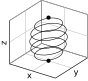
\includegraphics{Images/Поверхности 2 порядка/эллипсоид-z.png}
                \fi
            \end{center}
            Аналогично мы можем провернуть с остальными плоскостями (т.е. $y=\mathrm{const}$ и $x=\mathrm{const}$).
            \begin{center}
                \ifplotsrender
                \begin{tikzpicture}[every node/.style={scale=.625}]
                    \begin{axis}[
                        width = .3\textwidth,
                        height = .3\textwidth,
                        grid = major,
                        view={35}{30},
                        xmin = -5, xmax = 5,
                        ymin = -5, ymax = 5,
                        zmin = -5, zmax = 5,
                        xlabel = {$x$},
                        ylabel = {$y$},
                        zlabel = {$z$},
                        ticks = none,
                        ]
                        \foreach\h in {-8/3,-4/3,0,4/3,8/3}
                        {
                            \pgfmathparse{sqrt(1-(\h)^2/4^2)}
                            \let\s\pgfmathresult
                            \addplot3[domain=0:360,samples y=0]({3*\s*cos(x)},{\h},{5*\s*sin(x)});
                        }
                        \node[fill, shape=circle, fill, minimum size=5pt, inner sep=0pt] at (0,4,0) {};
                        \node[fill, shape=circle, fill, minimum size=5pt, inner sep=0pt] at (0,-4,0) {};
                    \end{axis}
                \end{tikzpicture}
                \begin{tikzpicture}[every node/.style={scale=.625}]
                    \begin{axis}[
                        width = .3\textwidth,
                        height = .3\textwidth,
                        grid = major,
                        view={35}{30},
                        xmin = -5, xmax = 5,
                        ymin = -5, ymax = 5,
                        zmin = -5, zmax = 5,
                        xlabel = {$x$},
                        ylabel = {$y$},
                        zlabel = {$z$},
                        ticks = none,
                        ]
                        \foreach\h in {-2,-1,0,1,2}
                        {
                            \pgfmathparse{sqrt(1-(\h)^2/3^2)}
                            \let\s\pgfmathresult
                            \addplot3[domain=0:360,samples y=0]({\h},{4*\s*sin(x)},{5*\s*cos(x)});
                        }
                        \node[fill, shape=circle, fill, minimum size=5pt, inner sep=0pt] at (3,0,0) {};
                        \node[fill, shape=circle, fill, minimum size=5pt, inner sep=0pt] at (-3,0,0) {};
                    \end{axis}
                \end{tikzpicture}
                \else
                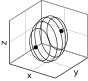
\includegraphics{Images/Поверхности 2 порядка/эллипсоид-y.png}
                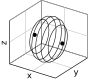
\includegraphics{Images/Поверхности 2 порядка/эллипсоид-x.png}
                \fi
            \end{center}
            Отсюда совершенно понятно, как выглядит получающаяся фигура.
            \begin{center}
                \ifplotsrender
                \begin{tikzpicture}[every node/.style={scale=.625}]
                    \begin{axis}[
                        width = .3\textwidth,
                        height = .3\textwidth,
                        grid = major,
                        view={35}{30},
                        z buffer=sort,
                        xmin = -5, xmax = 5,
                        ymin = -5, ymax = 5,
                        zmin = -5, zmax = 5,
                        xlabel = {$x$},
                        ylabel = {$y$},
                        zlabel = {$z$},
                        ticks = none,
                        colormap/cool,
                        ]
                        \addplot3[fill opacity=0.6,surf,domain=0:180,y domain=0:360]({3*sin(x)*cos(y)},{4*sin(x)*sin(y)},{5*cos(x)});
                    \end{axis}
                \end{tikzpicture}
                \else
                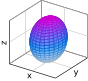
\includegraphics{Images/Поверхности 2 порядка/эллипсоид.png}
                \fi
            \end{center}
        \end{Example}
        \begin{Example}
            Рассмотрим однополостной гиперболоид $\frac{x^2}{a^2}+\frac{y^2}{b^2}-\frac{z^2}{c^2}=1$.\\
            Если мы рассматриваем плоскость $z=\mathrm{const}=h$, то мы опять получим эллиптические сечения, но с другими уравнениями $\frac{x^2}{a^2\left(1+\frac{h^2}{c^2}\right)}+\frac{y^2}{b^2\left(1+\frac{h^2}{c^2}\right)}=1$. Тут уже при росте $|h|$ полуоси эллипса растут, а в $h=0$ достигают минимума. Этот самый минимум именуют, кстати, горловым сечением.
            \begin{center}
                \ifplotsrender
                \begin{tikzpicture}[every node/.style={scale=.625}]
                    \begin{axis}[
                        width = .3\textwidth,
                        height = .3\textwidth,
                        grid = major,
                        view={35}{30},
                        xmin = -7, xmax = 7,
                        ymin = -7, ymax = 7,
                        zmin = -7, zmax = 7,
                        xlabel = {$x$},
                        ylabel = {$y$},
                        zlabel = {$z$},
                        ticks = none,
                        ]
                        \foreach\h in {-7,-14/3,-7/3}
                        {
                            \pgfmathparse{sqrt(1+(\h)^2/5^2)}
                            \let\s\pgfmathresult
                            \addplot3[domain=0:360,samples y=0]({3*\s*sin(x)},{4*\s*cos(x)},{\h});
                        }
                        \addplot3[domain=0:360,samples y=0,darkgreen,thick]({3*sin(x)},{4*cos(x)},{0});
                        \foreach\h in {7/3,14/3,7}
                        {
                            \pgfmathparse{sqrt(1+(\h)^2/5^2)}
                            \let\s\pgfmathresult
                            \addplot3[domain=0:360,samples y=0]({3*\s*sin(x)},{4*\s*cos(x)},{\h});
                        }
                    \end{axis}
                \end{tikzpicture}
                \else
                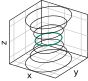
\includegraphics{Images/Поверхности 2 порядка/гиперболоид1-z.png}
                \fi
            \end{center}
            Теперь рассмотрим $y=\mathrm{const}=h$. Тогда мы получаем $\frac{x^2}{a^2\left(1-\frac{h^2}{b^2}\right)}-\frac{z^2}{c^2\left(1-\frac{h^2}{b^2}\right)}=1$. Но это только при $|h|<|b|$, и иначе $\frac{x^2}{a^2\left(\frac{h^2}{b^2}-1\right)}-\frac{z^2}{c^2\left(\frac{h^2}{b^2}-1\right)}=1$. То есть это две сопряжённых гиперболы. При $|h|=|b|$ мы получаем как раз асимптоты (т.е. две прямых).
            \begin{center}
                \ifplotsrender
                \begin{tikzpicture}[every node/.style={scale=.625}]
                    \begin{axis}[
                        width = .3\textwidth,
                        height = .3\textwidth,
                        grid = major,
                        view={35}{30},
                        xmin = -7, xmax = 7,
                        ymin = -7, ymax = 7,
                        zmin = -7, zmax = 7,
                        xlabel = {$x$},
                        ylabel = {$y$},
                        zlabel = {$z$},
                        ticks = none,
                        ]                        
                        \pgfmathparse{sqrt(abs(1-6^2/4^2))}
                        \let\s\pgfmathresult
                        \addplot3[domain=-4:4,samples y=0]({3*\s*sinh(x)},{6},{5*\s*cosh(x)});
                        \addplot3[domain=-4:4,samples y=0,restrict z to domain=-8:8]({3*\s*sinh(x)},{6},{-5*\s*cosh(x)});
                        \addplot3[darkgreen,thick,domain=-7:7,samples y=0,restrict z to domain=-8:8]({x},{4},{x*5/3});
                        \addplot3[darkgreen,thick,domain=-7:7,samples y=0]({x},{4},{-x*5/3});
                        \foreach\h in {2,0,-2}
                        {
                            \pgfmathparse{sqrt(abs(1-(\h)^2/4^2))}
                            \let\s\pgfmathresult
                            \addplot3[domain=-4:4,samples y=0]({3*\s*cosh(x)},{\h},{5*\s*sinh(x)});
                            \addplot3[domain=-4:4,samples y=0]({-3*\s*cosh(x)},{\h},{5*\s*sinh(x)});
                        }
                        \addplot3[darkgreen,thick,domain=-7:7,samples y=0]({x},{-4},{x*5/3});
                        \addplot3[darkgreen,thick,domain=-7:7,samples y=0]({x},{-4},{-x*5/3});
                        \pgfmathparse{sqrt(abs(1-6^2/4^2))}
                        \let\s\pgfmathresult
                        \addplot3[domain=-4:4,samples y=0,restrict z to domain=-9:9]({3*\s*sinh(x)},{-6},{5*\s*cosh(x)});
                        \addplot3[domain=-4:4,samples y=0]({3*\s*sinh(x)},{-6},{-5*\s*cosh(x)});
                    \end{axis}
                \end{tikzpicture}
                \begin{tikzpicture}[every node/.style={scale=.625}]
                    \begin{axis}[
                        width = .3\textwidth,
                        height = .3\textwidth,
                        grid = major,
                        view={35}{30},
                        xmin = -7, xmax = 7,
                        ymin = -7, ymax = 7,
                        zmin = -7, zmax = 7,
                        xlabel = {$x$},
                        ylabel = {$y$},
                        zlabel = {$z$},
                        ticks = none,
                        ]                        
                        \foreach\h in {-6,-5,-4}
                        {
                            \pgfmathparse{sqrt(abs(1-(\h)^2/3^2))}
                            \let\s\pgfmathresult
                            \addplot3[domain=-3:3,samples y=0,restrict z to domain=-8:8]({\h},{4*\s*sinh(x)},{5*\s*cosh(x)});
                            \addplot3[domain=-3:3,samples y=0,restrict z to domain=-8:8]({\h},{4*\s*sinh(x)},{-5*\s*cosh(x)});
                        }
                        \addplot3[darkgreen,thick,domain=-7:7,samples y=0,restrict z to domain=-8:8]({3},{x},{x*5/4});
                        \addplot3[darkgreen,thick,domain=-7:7,samples y=0,restrict z to domain=-8:8]({3},{x},{-x*5/4});
                        \foreach\h in {2,1,0,1,-2}
                        {
                            \pgfmathparse{sqrt(abs(1-(\h)^2/3^2))}
                            \let\s\pgfmathresult
                            \addplot3[domain=-3:3,samples y=0]({\h},{4*\s*cosh(x)},{5*\s*sinh(x)});
                            \addplot3[domain=-3:3,samples y=0]({\h},{-4*\s*cosh(x)},{5*\s*sinh(x)});
                        }
                        \addplot3[darkgreen,thick,domain=-7:7,samples y=0,restrict z to domain=-8:8]({-3},{x},{x*5/4});
                        \addplot3[darkgreen,thick,domain=-7:7,samples y=0,restrict z to domain=-8:8]({-3},{x},{-x*5/4});
                        \foreach\h in {4,5,6}
                        {
                            \pgfmathparse{sqrt(abs(1-(\h)^2/3^2))}
                            \let\s\pgfmathresult
                            \addplot3[domain=-3:3,samples y=0,restrict z to domain=-8:8]({\h},{4*\s*sinh(x)},{5*\s*cosh(x)});
                            \addplot3[domain=-3:3,samples y=0,restrict z to domain=-8:8]({\h},{4*\s*sinh(x)},{-5*\s*cosh(x)});
                        }
                    \end{axis}
                \end{tikzpicture}
                \else
                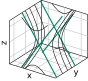
\includegraphics{Images/Поверхности 2 порядка/гиперболоид1-y.png}
                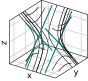
\includegraphics{Images/Поверхности 2 порядка/гиперболоид1-x.png}
                \fi
            \end{center}
            Отсюда уже не так очевидно, но всё ещё можно понять, как выглядит итоговая фигура.
            \begin{center}
                \ifplotsrender
                \begin{tikzpicture}[every node/.style={scale=.625}]
                    \begin{axis}[
                        width = .3\textwidth,
                        height = .3\textwidth,
                        grid = major,
                        view={35}{30},
                        z buffer=sort,
                        xmin = -7, xmax = 7,
                        ymin = -7, ymax = 7,
                        zmin = -7, zmax = 7,
                        xlabel = {$x$},
                        ylabel = {$y$},
                        zlabel = {$z$},
                        ticks = none,
                        colormap/cool,
                        ]
                        \addplot3[fill opacity=0.6,surf,domain=-7/5:7/5,y domain=0:360]({3*(cos(y)-x*sin(y))},{4*(sin(y)+x*cos(y))},{5*x});
                        \addplot3[fill opacity=0.6,surf,domain=-7/5:7/5,y domain=0:360]({3*(cos(y)-x*sin(y))},{4*(sin(y)+x*cos(y))},{-5*x});
                    \end{axis}
                \end{tikzpicture}
                \else
                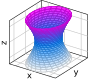
\includegraphics{Images/Поверхности 2 порядка/гиперболоид1.png}
                \fi
            \end{center}
        \end{Example}
        \begin{Example}
            Рассмотрим теперь двуполостной гиперболоид $\frac{x^2}{a^2}+\frac{y^2}{b^2}-\frac{z^2}{c^2}=-1$.\\
            Плоскости $z=\mathrm{const}=h$ опять дают нам эллиптические сечения с уравнениями $\frac{x^2}{a^2\left(-1+\frac{h^2}{c^2}\right)}+\frac{y^2}{b^2\left(-1+\frac{h^2}{c^2}\right)}=1$. Тут уже при росте $|h|$ полуоси эллипса всё ещё растут, но при $h\in(-c;c)$ это не эллипсы, а пустые множества. При $h=\pm c$ сечение явялется точкой с нулевой абсциссой и ординатой.
            \begin{center}
                \ifplotsrender
                \begin{tikzpicture}[every node/.style={scale=.625}]
                    \begin{axis}[
                        width = .3\textwidth,
                        height = .3\textwidth,
                        grid = major,
                        view={35}{30},
                        xmin = -7, xmax = 7,
                        ymin = -7, ymax = 7,
                        zmin = -7, zmax = 7,
                        xlabel = {$x$},
                        ylabel = {$y$},
                        zlabel = {$z$},
                        ticks = none,
                        ]
                        \foreach\h in {-7,-6}
                        {
                            \pgfmathparse{sqrt(-1+(\h)^2/5^2)}
                            \let\s\pgfmathresult
                            \addplot3[domain=0:360,samples y=0]({3*\s*sin(x)},{4*\s*cos(x)},{\h});
                        }
                        \node[fill, shape=circle, fill, minimum size=5pt, inner sep=0pt] at (0,0,5) {};
                        \node[fill, shape=circle, fill, minimum size=5pt, inner sep=0pt] at (0,0,-5) {};
                        \foreach\h in {6,7}
                        {
                            \pgfmathparse{sqrt(-1+(\h)^2/5^2)}
                            \let\s\pgfmathresult
                            \addplot3[domain=0:360,samples y=0]({3*\s*sin(x)},{4*\s*cos(x)},{\h});
                        }
                    \end{axis}
                \end{tikzpicture}
                \else
                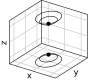
\includegraphics{Images/Поверхности 2 порядка/гиперболоид2-z.png}
                \fi
            \end{center}
            Рассмотрим $y=\mathrm{const}=h$. Тогда мы получаем $-\frac{x^2}{a^2\left(1+\frac{h^2}{b^2}\right)}+\frac{z^2}{c^2\left(1+\frac{h^2}{b^2}\right)}=1$. Тут уже нет случаев $|h|<|b|$ и $|h|>|b|$, мы просто имеем гиперболы, которые тем дальше от асимптот, чем больше $|h|$ по модулю. При этом до самих асимптот (в отличие от однополостного гиперболоида) эти гиперболы никогда не дойдут.
            \begin{center}
                \ifplotsrender
                \begin{tikzpicture}[every node/.style={scale=.625}]
                    \begin{axis}[
                        width = .3\textwidth,
                        height = .3\textwidth,
                        grid = major,
                        view={35}{30},
                        xmin = -7, xmax = 7,
                        ymin = -7, ymax = 7,
                        zmin = -7, zmax = 7,
                        xlabel = {$x$},
                        ylabel = {$y$},
                        zlabel = {$z$},
                        ticks = none,
                        ]
                        \foreach\h in {-7,...,7}
                        {
                            \pgfmathparse{sqrt(1+(\h)^2/4^2)}
                            \let\s\pgfmathresult
                            \addplot3[domain=-4:4,samples y=0,restrict z to domain=-8:8]({3*\s*sinh(x)},{\h},{5*\s*cosh(x)});
                            \addplot3[domain=-4:4,samples y=0,restrict z to domain=-8:8]({3*\s*sinh(x)},{\h},{-5*\s*cosh(x)});
                        }
                    \end{axis}
                \end{tikzpicture}
                \begin{tikzpicture}[every node/.style={scale=.625}]
                    \begin{axis}[
                        width = .3\textwidth,
                        height = .3\textwidth,
                        grid = major,
                        view={35}{30},
                        xmin = -7, xmax = 7,
                        ymin = -7, ymax = 7,
                        zmin = -7, zmax = 7,
                        xlabel = {$x$},
                        ylabel = {$y$},
                        zlabel = {$z$},
                        ticks = none,
                        ]
                        \foreach\h in {-7,...,7}
                        {
                            \pgfmathparse{sqrt(1+(\h)^2/3^2)}
                            \let\s\pgfmathresult
                            \addplot3[domain=-4:4,samples y=0,restrict z to domain=-8:8]({\h},{4*\s*sinh(x)},{5*\s*cosh(x)});
                            \addplot3[domain=-4:4,samples y=0,restrict z to domain=-8:8]({\h},{4*\s*sinh(x)},{-5*\s*cosh(x)});
                        }
                    \end{axis}
                \end{tikzpicture}
                \else
                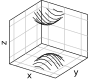
\includegraphics{Images/Поверхности 2 порядка/гиперболоид2-y.png}
                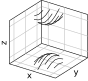
\includegraphics{Images/Поверхности 2 порядка/гиперболоид2-x.png}
                \fi
            \end{center}
            Итоговая фигура выглядит так:
            \begin{center}
                \ifplotsrender
                \begin{tikzpicture}[every node/.style={scale=.625}]
                    \begin{axis}[
                        width = .3\textwidth,
                        height = .3\textwidth,
                        grid = major,
                        view={35}{30},
                        z buffer=sort,
                        xmin = -7, xmax = 7,
                        ymin = -7, ymax = 7,
                        zmin = -7, zmax = 7,
                        xlabel = {$x$},
                        ylabel = {$y$},
                        zlabel = {$z$},
                        ticks = none,
                        colormap/cool,
                        ]
                        \addplot3[fill opacity=0.6,surf,domain=0:7/5,y domain=0:360]({3*sinh(x)*cos(y)},{4*sinh(x)*sin(y)},{5*cosh(x)});
                        \addplot3[fill opacity=0.6,surf,domain=0:7/5,y domain=0:360]({3*sinh(x)*cos(y)},{4*sinh(x)*sin(y)},{-5*cosh(x)});
                    \end{axis}
                \end{tikzpicture}
                \else
                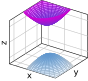
\includegraphics{Images/Поверхности 2 порядка/гиперболоид2.png}
                \fi
            \end{center}
        \end{Example}
        \dfn Если у гиперболоида коэффициенты $a$ и $b$ равны, то он называется \undercolor{red}{гиперболоидом вращения}.
        \ifplotsrender
        \pagebreak
        \fi
        \begin{Example}
            Конус. $\frac{x^2}{a^2}+\frac{y^2}{b^2}=\frac{z^2}{c^2}$.\\
            Плоскости $z=\mathrm{const}=h$ дают эллиптические сечения с уравнениями $\frac{x^2}{a^2\left(\frac{h^2}{c^2}\right)}+\frac{y^2}{b^2\left(\frac{h^2}{c^2}\right)}=1$, то есть как при однополостном гиперболоиде, но при $h=0$ получается точка.
            \begin{center}
                \ifplotsrender
                \begin{tikzpicture}[every node/.style={scale=.625}]
                    \begin{axis}[
                        width = .3\textwidth,
                        height = .3\textwidth,
                        grid = major,
                        view={35}{30},
                        xmin = -7, xmax = 7,
                        ymin = -7, ymax = 7,
                        zmin = -7, zmax = 7,
                        xlabel = {$x$},
                        ylabel = {$y$},
                        zlabel = {$z$},
                        ticks = none,
                        ]
                        \foreach\h in {-7,-21/4,-7/2,-7/4}
                        {
                            \pgfmathparse{sqrt((\h)^2/5^2)}
                            \let\s\pgfmathresult
                            \addplot3[domain=0:360,samples y=0]({3*\s*sin(x)},{4*\s*cos(x)},{\h});
                        }
                        \node[fill, shape=circle, fill, minimum size=5pt, inner sep=0pt] at (0,0,0) {};
                        \foreach\h in {7/4,7/2,21/4,7}
                        {
                            \pgfmathparse{sqrt((\h)^2/5^2)}
                            \let\s\pgfmathresult
                            \addplot3[domain=0:360,samples y=0]({3*\s*sin(x)},{4*\s*cos(x)},{\h});
                        }
                    \end{axis}
                \end{tikzpicture}
                \else
                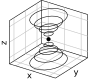
\includegraphics{Images/Поверхности 2 порядка/конус-z.png}
                \fi
            \end{center}
            Рассмотрим $y=\mathrm{const}=h$. Тогда мы получаем $-\frac{x^2}{a^2\left(\frac{h^2}{b^2}\right)}+\frac{z^2}{c^2\left(\frac{h^2}{b^2}\right)}=1$. Как в случае гиперболоидов, это гиперболы, но тут случай промежуточный между разными гиперболоидами. Сечение может только в одном случае ($h=0$) превратится в асимптоты гипербол, а никаких сопряжённых гипербол тут нет.
            \begin{center}
                \ifplotsrender
                \begin{tikzpicture}[every node/.style={scale=.625}]
                    \begin{axis}[
                        width = .3\textwidth,
                        height = .3\textwidth,
                        grid = major,
                        view={35}{30},
                        xmin = -7, xmax = 7,
                        ymin = -7, ymax = 7,
                        zmin = -7, zmax = 7,
                        xlabel = {$x$},
                        ylabel = {$y$},
                        zlabel = {$z$},
                        ticks = none,
                        ]                        
                        \foreach\h in {-6,-4,-2}
                        {
                            \pgfmathparse{sqrt((\h)^2/4^2)}
                            \let\s\pgfmathresult
                            \addplot3[domain=-3:3,samples y=0,restrict z to domain=-8:8]({3*\s*sinh(x)},{\h},{5*\s*cosh(x)});
                            \addplot3[domain=-3:3,samples y=0,restrict z to domain=-8:8]({3*\s*sinh(x)},{\h},{-5*\s*cosh(x)});
                        }
                        \addplot3[darkgreen,thick,domain=-7:7,samples y=0,restrict z to domain=-8:8]({x},{0},{x*5/3});
                        \addplot3[darkgreen,thick,domain=-7:7,samples y=0,restrict z to domain=-8:8]({x},{0},{-x*5/3});
                        \foreach\h in {2,4,6}
                        {
                            \pgfmathparse{sqrt((\h)^2/4^2)}
                            \let\s\pgfmathresult
                            \addplot3[domain=-3:3,samples y=0,restrict z to domain=-8:8]({3*\s*sinh(x)},{\h},{5*\s*cosh(x)});
                            \addplot3[domain=-3:3,samples y=0,restrict z to domain=-8:8]({3*\s*sinh(x)},{\h},{-5*\s*cosh(x)});
                        }
                    \end{axis}
                \end{tikzpicture}
                \begin{tikzpicture}[every node/.style={scale=.625}]
                    \begin{axis}[
                        width = .3\textwidth,
                        height = .3\textwidth,
                        grid = major,
                        view={35}{30},
                        xmin = -7, xmax = 7,
                        ymin = -7, ymax = 7,
                        zmin = -7, zmax = 7,
                        xlabel = {$x$},
                        ylabel = {$y$},
                        zlabel = {$z$},
                        ticks = none,
                        ]                        
                        \foreach\h in {-4,-3,-2,-1}
                        {
                            \pgfmathparse{sqrt((\h)^2/3^2)}
                            \let\s\pgfmathresult
                            \addplot3[domain=-3:3,samples y=0,restrict z to domain=-8:8]({\h},{4*\s*sinh(x)},{5*\s*cosh(x)});
                            \addplot3[domain=-3:3,samples y=0,restrict z to domain=-8:8]({\h},{4*\s*sinh(x)},{-5*\s*cosh(x)});
                        }
                        \addplot3[darkgreen,thick,domain=-7:7,samples y=0,restrict z to domain=-8:8]({0},{x},{x*5/4});
                        \addplot3[darkgreen,thick,domain=-7:7,samples y=0,restrict z to domain=-8:8]({0},{x},{-x*5/4});
                        \foreach\h in {1,2,3,4}
                        {
                            \pgfmathparse{sqrt((\h)^2/3^2)}
                            \let\s\pgfmathresult
                            \addplot3[domain=-3:3,samples y=0,restrict z to domain=-8:8]({\h},{4*\s*sinh(x)},{5*\s*cosh(x)});
                            \addplot3[domain=-3:3,samples y=0,restrict z to domain=-8:8]({\h},{4*\s*sinh(x)},{-5*\s*cosh(x)});
                        }
                    \end{axis}
                \end{tikzpicture}
                \else
                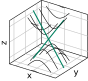
\includegraphics{Images/Поверхности 2 порядка/конус-y.png}
                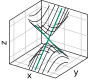
\includegraphics{Images/Поверхности 2 порядка/конус-x.png}
                \fi
            \end{center}
            Никто никогда не видел конус в своей жизни, поэтому вот он:
            \begin{center}
                \ifplotsrender
                \begin{tikzpicture}[every node/.style={scale=.625}]
                    \begin{axis}[
                        width = .3\textwidth,
                        height = .3\textwidth,
                        grid = major,
                        view={35}{30},
                        z buffer=sort,
                        xmin = -7, xmax = 7,
                        ymin = -7, ymax = 7,
                        zmin = -7, zmax = 7,
                        xlabel = {$x$},
                        ylabel = {$y$},
                        zlabel = {$z$},
                        ticks = none,
                        colormap/cool,
                        ]
                        \addplot3[fill opacity=0.6,surf,domain=-7/5:7/5,y domain=0:360]({3*x*cos(y)},{4*x*sin(y)},{5*x});
                    \end{axis}
                \end{tikzpicture}
                \else
                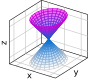
\includegraphics{Images/Поверхности 2 порядка/конус.png}
                \fi
            \end{center}
        \end{Example}
        \dfn По аналогии с гиперболоидом, если у конуса равны коэффициенты $a$ и $b$, то он называется \undercolor{red}{конусом вращения}.
        \thm Конус является объединением пучка прямых, проходящих через начало координат.
        \ifplotsrender
        \else
        \pagebreak
        \fi
        \begin{Proof}
            Возьмём уравнение конуса $\frac{x^2}{a^2}+\frac{y^2}{b^2}=\frac{z^2}{c^2}$. Рассмотрим точку конуса $(x_0;y_0;z_0)$. Рассмотрим прямую, проходящую через эту точку и начало координат. Её можно записать как $\{(x_0t;y_0t;z_0t)\mid t\in\mathbb R\}$. Подставим любую точку этой прямой в уравнение конуса. $\frac{x_0^2t^2}{a^2}+\frac{y_0^2t^2}{b^2}=\frac{z_0^2t^2}{c^2}$. Несложно заметить, что можно поделить на $t^2$. Получим верное равенство, так как точка $(x_0;y_0;z_0)$ по построению принадлежит конусу.
            \begin{center}
                \ifplotsrender
                \begin{tikzpicture}[every node/.style={scale=.625}]
                    \begin{axis}[
                        width = .3\textwidth,
                        height = .3\textwidth,
                        grid = major,
                        view={35}{30},
                        xmin = -7, xmax = 7,
                        ymin = -7, ymax = 7,
                        zmin = -7, zmax = 7,
                        xlabel = {$x$},
                        ylabel = {$y$},
                        zlabel = {$z$},
                        ticks = none,
                        ]
                        \foreach\h in {0,30,60,90,120,150,180,210,240,270,300,330}
                        {
                            \addplot3[domain=-7/5:7/5,samples y=0,restrict z to domain=-8:8]({3*x*cos(\h)},{4*x*sin(\h)},{5*x});
                        }
                    \end{axis}
                \end{tikzpicture}
                \else
                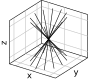
\includegraphics{Images/Поверхности 2 порядка/конус-addon.png}
                \fi
            \end{center}
        \end{Proof}
        \dfn Эти прямые называются \undercolor{red}{образующими}.
        \thm Для каждой из трёх типов невырожденных кривый второго порядка конус содержит сечение, являющееся кривой этого типа.
        \begin{Proof}
            Эллипс и гиперболу мы уже получили. Осталось получить параболу. Для этого можно взять плоскость, параллельную одной из образующих прямых. Доказывать, что это парабола, мы, разумеется, не будем.
            \begin{center}
                \ifplotsrender
                \begin{tikzpicture}[every node/.style={scale=.625}]
                    \begin{axis}[
                        width = .3\textwidth,
                        height = .3\textwidth,
                        grid = major,
                        view={35}{30},
                        xmin = -7, xmax = 7,
                        ymin = -7, ymax = 7,
                        zmin = -7, zmax = 7,
                        xlabel = {$x$},
                        ylabel = {$y$},
                        zlabel = {$z$},
                        ticks = none,
                        colormap/cool,
                        ]
                        \addplot3[fill opacity=0.6,surf,domain=-7/5:7/5,y domain=0:360,z buffer=sort]({3*x*cos(y)},{4*x*sin(y)},{5*x});
                        \addplot3[black,thick,domain=-7:8/5,samples y=0]({3*sqrt(-10*x+16)/5},{x},{5*x/4-4});
                        \addplot3[black,thick,dashed,domain=-7:8/5,samples y=0]({-3*sqrt(-10*x+16)/5},{x},{5*x/4-4});
                        \addplot3[fill opacity=0.2,surf,red,samples=2,domain=-7:7]{5*y/4-4};
                    \end{axis}
                \end{tikzpicture}
                \else
                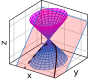
\includegraphics{Images/Поверхности 2 порядка/конус-addon2.png}
                \fi
            \end{center}
        \end{Proof}
        \begin{Comment}
            Кстати, это единственная поверхность второго порядка с этим свойством.
        \end{Comment}
        \begin{Example}
            Параболоиды. Сначала эллиптический $\frac{x^2}{2p}+\frac{y^2}{2q}=z$.\\
            Плоскость $z=\mathrm{const}=h$. Получается уравнение $\frac{x^2}{2ph}+\frac{y^2}{2qh}=1$. При $h=0$ это точка $(0;0;0)$. При $h<0$ это пустое множество, при положительном $h$ --- эллипсы. Причём чем больше $h$, тем больше полуоси.
            \begin{center}
                \ifplotsrender
                \begin{tikzpicture}[every node/.style={scale=.625}]
                    \begin{axis}[
                        width = .3\textwidth,
                        height = .3\textwidth,
                        grid = major,
                        view={35}{30},
                        xmin = -7, xmax = 7,
                        ymin = -7, ymax = 7,
                        zmin = -7, zmax = 7,
                        xlabel = {$x$},
                        ylabel = {$y$},
                        zlabel = {$z$},
                        ticks = none,
                        ]
                        \node[fill, shape=circle, fill, minimum size=5pt, inner sep=0pt] at (0,0,0) {};
                        \foreach\h in {7/4,7/2,21/4,7}
                        {
                            \addplot3[domain=0:360,samples y=0,restrict z to domain=-8:8]({cos(x)*sqrt(4*\h)},{sin(x)*sqrt(6*\h)},{\h});
                        }
                    \end{axis}
                \end{tikzpicture}
                \else
                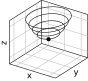
\includegraphics{Images/Поверхности 2 порядка/параболоид1-z.png}
                \fi
            \end{center}
            Рассмотрим $y=\mathrm{const}=h$. Тогда мы получаем $\frac{x^2}{2p}+\frac{h^2}{2q}=z$. Это парабола, которую мы просто подвинули в сторону оси $y$. Причём тем выше, чем больше $|h|$. При $h=0$ это парабола с вершиной в нуле. Аналогично с $x=\mathrm{const}$.
            \begin{center}
                \ifplotsrender
                \begin{tikzpicture}[every node/.style={scale=.625}]
                    \begin{axis}[
                        width = .3\textwidth,
                        height = .3\textwidth,
                        grid = major,
                        view={35}{30},
                        xmin = -7, xmax = 7,
                        ymin = -7, ymax = 7,
                        zmin = -7, zmax = 7,
                        xlabel = {$x$},
                        ylabel = {$y$},
                        zlabel = {$z$},
                        ticks = none,
                        ]
                        \foreach\h in {7/4,7/2,21/4,7}
                        {
                            \addplot3[domain=-7:7,samples y=0,restrict z to domain=-8:8]({x},{\h},{x^2/4+(\h)^2/6});
                        }
                        \addplot3[darkgreen,thick,domain=-7:7,samples y=0,restrict z to domain=-8:8]({x},{0},{x^2/4});
                        \foreach\h in {-7/4,-7/2,-21/4,-7}
                        {
                            \addplot3[domain=-7:7,samples y=0,restrict z to domain=-8:8]({x},{\h},{x^2/4+(\h)^2/6});
                        }
                    \end{axis}
                \end{tikzpicture}
                \begin{tikzpicture}[every node/.style={scale=.625}]
                    \begin{axis}[
                        width = .3\textwidth,
                        height = .3\textwidth,
                        grid = major,
                        view={35}{30},
                        xmin = -7, xmax = 7,
                        ymin = -7, ymax = 7,
                        zmin = -7, zmax = 7,
                        xlabel = {$x$},
                        ylabel = {$y$},
                        zlabel = {$z$},
                        ticks = none,
                        ]
                        \foreach\h in {-7/4,-7/2,-21/4,-7}
                        {
                            \addplot3[domain=-7:7,samples y=0,restrict z to domain=-8:8]({\h},{x},{(\h)^2/4+x^2/6});
                        }
                        \addplot3[darkgreen,thick,domain=-7:7,samples y=0,restrict z to domain=-8:8]({0},{x},{x^2/6});
                        \foreach\h in {7/4,7/2,21/4,7}
                        {
                            \addplot3[domain=-7:7,samples y=0,restrict z to domain=-8:8]({\h},{x},{(\h)^2/4+x^2/6});
                        }
                    \end{axis}
                \end{tikzpicture}
                \else
                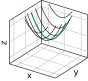
\includegraphics{Images/Поверхности 2 порядка/параболоид1-y.png}
                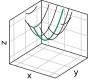
\includegraphics{Images/Поверхности 2 порядка/параболоид1-x.png}
                \fi
            \end{center}
            Параболоид выглядит так:
            \begin{center}
                \ifplotsrender
                \begin{tikzpicture}[every node/.style={scale=.625}]
                    \begin{axis}[
                        width = .3\textwidth,
                        height = .3\textwidth,
                        grid = major,
                        view={35}{30},
                        z buffer=sort,
                        xmin = -7, xmax = 7,
                        ymin = -7, ymax = 7,
                        zmin = -7, zmax = 7,
                        xlabel = {$x$},
                        ylabel = {$y$},
                        zlabel = {$z$},
                        ticks = none,
                        colormap/cool, 
                        ]
                        \addplot3[fill opacity=0.6,surf,domain=0:7,domain y=0:360]({cos(y)*2*sqrt(x)},{sin(y)*sqrt(6)*sqrt(x)},{x});
                    \end{axis}
                \end{tikzpicture}
                \else
                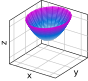
\includegraphics{Images/Поверхности 2 порядка/параболоид1.png}
                \fi
            \end{center}
            Заметим интересный факт. Мы можем считать, что эллиптический параболоид получается движением одной параболы по другой. А точнее, если взять, например, параболу при $y=0$ и откладывать её вершину от точек параболы $x=\mathrm{const}$, то мы получим именно то, что нам надо.
            \begin{center}
                \ifplotsrender
                \begin{tikzpicture}[every node/.style={scale=.625}]
                    \begin{axis}[
                        width = .3\textwidth,
                        height = .3\textwidth,
                        grid = major,
                        view={35}{30},
                        xmin = -7, xmax = 7,
                        ymin = -7, ymax = 7,
                        zmin = -7, zmax = 7,
                        xlabel = {$x$},
                        ylabel = {$y$},
                        zlabel = {$z$},
                        ticks = none,
                        ]
                        \addplot3[darkgreen,thick,domain=-7:7,samples y=0,restrict z to domain=-8:8]({x},{0},{x^2/4});
                        \foreach\h in {-14/3,-7/3,0,7/3,14/3}
                        {
                            \addplot3[domain=-7:7,samples y=0,restrict z to domain=-8:8]({\h},{x},{(\h)^2/4+x^2/6});
                        }
                        \node[fill, shape=circle, fill, minimum size=3pt, inner sep=0pt] at (-14/3,0,14*14/3/3/4) {};
                        \node[fill, shape=circle, fill, minimum size=3pt, inner sep=0pt] at (-7/3,0,7*7/3/3/4) {};
                        \node[fill, shape=circle, fill, minimum size=3pt, inner sep=0pt] at (0,0,0) {};
                        \node[fill, shape=circle, fill, minimum size=3pt, inner sep=0pt] at (7/3,0,7*7/3/3/4) {};
                        \node[fill, shape=circle, fill, minimum size=3pt, inner sep=0pt] at (14/3,0,14*14/3/3/4) {};
                    \end{axis}
                \end{tikzpicture}
                \else
                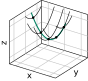
\includegraphics{Images/Поверхности 2 порядка/параболоид1-addon.png}
                \fi
            \end{center}
        \end{Example}
        \begin{Example}
            Теперь гиперболический параболоид $\frac{x^2}{2p}-\frac{y^2}{2q}=z$.\\
            При сечении плоскостью $z=\mathrm{const}=h$ получается гипербола $\frac{x^2}{2ph}-\frac{y^2}{2qh}=1$. При $h=0$ это не гипербола, это её асимптоты. При этом для $h$ разных знаков мы получаем сопряжённые гиперболы. Также заметим, что с ростом $|h|$ получаются гиперболы, всё более далёкие от асимптот.
            \begin{center}
                \ifplotsrender
                \begin{tikzpicture}[every node/.style={scale=.625}]
                    \begin{axis}[
                        width = .3\textwidth,
                        height = .3\textwidth,
                        grid = major,
                        view={35}{30},
                        xmin = -7, xmax = 7,
                        ymin = -7, ymax = 7,
                        zmin = -7, zmax = 7,
                        xlabel = {$x$},
                        ylabel = {$y$},
                        zlabel = {$z$},
                        ticks = none,
                        ]
                        \foreach\h in {-7/4,-7/2,-21/4,-7}
                        {
                            \addplot3[domain=-3:3,samples y=0,restrict x to domain=-8:8,restrict y to domain=-8:8,restrict z to domain=-8:8]({sinh(x)*sqrt(-6*\h)},{cosh(x)*sqrt(-4*\h)},{\h});
                            \addplot3[domain=-3:3,samples y=0,restrict x to domain=-8:8,restrict y to domain=-8:8,restrict z to domain=-8:8]({sinh(x)*sqrt(-6*\h)},{-cosh(x)*sqrt(-4*\h)},{\h});
                        }
                        \addplot3[darkgreen,thick,domain=-3:3,samples y=0,restrict x to domain=-8:8,restrict y to domain=-8:8,restrict z to domain=-8:8]({sqrt(6)*x},{sqrt(4)*x},{0});
                        \addplot3[darkgreen,thick,domain=-3:3,samples y=0,restrict x to domain=-8:8,restrict y to domain=-8:8,restrict z to domain=-8:8]({sqrt(6)*x},{-sqrt(4)*x},{0});
                        \foreach\h in {7/4,7/2,21/4,7}
                        {
                            \addplot3[domain=-3:3,samples y=0,restrict x to domain=-8:8,restrict y to domain=-8:8,restrict z to domain=-8:8]({cosh(x)*sqrt(6*\h)},{sinh(x)*sqrt(4*\h)},{\h});
                            \addplot3[domain=-3:3,samples y=0,restrict x to domain=-8:8,restrict y to domain=-8:8,restrict z to domain=-8:8]({-cosh(x)*sqrt(6*\h)},{sinh(x)*sqrt(4*\h)},{\h});
                        }
                    \end{axis}
                \end{tikzpicture}
                \else
                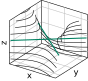
\includegraphics{Images/Поверхности 2 порядка/параболоид2-z.png}
                \fi
            \end{center}
            Рассмотрим $y=\mathrm{const}=h$. Тут получаем $\frac{x^2}{2p}-\frac{h^2}{2q}=z$. Это всё ещё парабола, Но её мы уже двигаем сторону напротив оси $y$. И опять тем дальше, чем больше $|h|$. При $h=0$ это, как и в эллиптическом параболоиде, парабола с вершиной в нуле. С $x=\mathrm{const}$ получается аналогично, но тут уже параболы едут вдоль оси $x$ при росте параметра, а не против её.
            \begin{center}
                \ifplotsrender
                \begin{tikzpicture}[every node/.style={scale=.625}]
                    \begin{axis}[
                        width = .3\textwidth,
                        height = .3\textwidth,
                        grid = major,
                        view={35}{30},
                        xmin = -7, xmax = 7,
                        ymin = -7, ymax = 7,
                        zmin = -7, zmax = 7,
                        xlabel = {$x$},
                        ylabel = {$y$},
                        zlabel = {$z$},
                        ticks = none,
                        ]
                        \foreach\h in {-7/4,-7/2,-21/4,-7}
                        {
                            \addplot3[domain=-7:7,samples y=0,restrict z to domain=-8:8]({x},{\h},{x^2/6-(\h)^2/4});
                        }
                        \addplot3[darkgreen,thick,domain=-7:7,samples y=0,restrict z to domain=-8:8]({x},{0},{x^2/6});
                        \foreach\h in {7/4,7/2,21/4,7}
                        {
                            \addplot3[domain=-7:7,samples y=0,restrict z to domain=-8:8]({x},{\h},{x^2/6-(\h)^2/4});
                        }
                    \end{axis}
                \end{tikzpicture}
                \begin{tikzpicture}[every node/.style={scale=.625}]
                    \begin{axis}[
                        width = .3\textwidth,
                        height = .3\textwidth,
                        grid = major,
                        view={35}{30},
                        xmin = -7, xmax = 7,
                        ymin = -7, ymax = 7,
                        zmin = -7, zmax = 7,
                        xlabel = {$x$},
                        ylabel = {$y$},
                        zlabel = {$z$},
                        ticks = none,
                        ]
                        \foreach\h in {-7/4,-7/2,-21/4,-7}
                        {
                            \addplot3[domain=-7:7,samples y=0,restrict z to domain=-8:8]({\h},{x},{(\h)^2/6-x^2/4});
                        }
                        \addplot3[darkgreen,thick,domain=-7:7,samples y=0,restrict z to domain=-8:8]({0},{x},{-x^2/4});
                        \foreach\h in {7/4,7/2,21/4,7}
                        {
                            \addplot3[domain=-7:7,samples y=0,restrict z to domain=-8:8]({\h},{x},{(\h)^2/6-x^2/4});
                        }
                    \end{axis}
                \end{tikzpicture}
                \else
                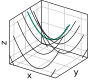
\includegraphics{Images/Поверхности 2 порядка/параболоид2-y.png}
                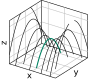
\includegraphics{Images/Поверхности 2 порядка/параболоид2-x.png}
                \fi
            \end{center}
            Сам гиперболический параболоид выглядит так:
            \begin{center}
                \ifplotsrender
                \begin{tikzpicture}[every node/.style={scale=.625}]
                    \begin{axis}[
                        width = .3\textwidth,
                        height = .3\textwidth,
                        grid = major,
                        view={35}{30},
                        z buffer=sort,
                        xmin = -7, xmax = 7,
                        ymin = -7, ymax = 7,
                        zmin = -7, zmax = 7,
                        xlabel = {$x$},
                        ylabel = {$y$},
                        zlabel = {$z$},
                        ticks = none,
                        colormap/cool,
                        ]
                        \addplot3[domain=-7:7,surf]{x^2/6-y^2/4};
                    \end{axis}
                \end{tikzpicture}
                \else
                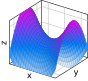
\includegraphics{Images/Поверхности 2 порядка/параболоид2.png}
                \fi
            \end{center}
            Про гиперболический параболоид есть такой же интересный факт, что и про эллиптический. Он получается движением одной параболы по другой. Но если в случае с эллиптическим у обеих ветви были в одну сторону (вверх), то теперь --- в разные.
            \begin{center}
                \ifplotsrender
                \begin{tikzpicture}[every node/.style={scale=.625}]
                    \begin{axis}[
                        width = .3\textwidth,
                        height = .3\textwidth,
                        grid = major,
                        view={35}{30},
                        xmin = -7, xmax = 7,
                        ymin = -7, ymax = 7,
                        zmin = -7, zmax = 7,
                        xlabel = {$x$},
                        ylabel = {$y$},
                        zlabel = {$z$},
                        ticks = none,
                        ]
                        \addplot3[darkgreen,thick,domain=-7:7,samples y=0,restrict z to domain=-8:8]({x},{0},{x^2/6});
                        \foreach\h in {-14/3,-7/3,0,7/3,14/3}
                        {
                            \addplot3[domain=-7:7,samples y=0,restrict z to domain=-8:8]({\h},{x},{(\h)^2/6-x^2/4});
                        }
                        \node[fill, shape=circle, fill, minimum size=3pt, inner sep=0pt] at (-14/3,0,14*14/3/3/6) {};
                        \node[fill, shape=circle, fill, minimum size=3pt, inner sep=0pt] at (-7/3,0,7*7/3/3/6) {};
                        \node[fill, shape=circle, fill, minimum size=3pt, inner sep=0pt] at (0,0,0) {};
                        \node[fill, shape=circle, fill, minimum size=3pt, inner sep=0pt] at (7/3,0,7*7/3/3/6) {};
                        \node[fill, shape=circle, fill, minimum size=3pt, inner sep=0pt] at (14/3,0,14*14/3/3/6) {};
                    \end{axis}
                \end{tikzpicture}
                \else
                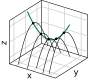
\includegraphics{Images/Поверхности 2 порядка/параболоид2-addon.png}
                \fi
            \end{center}
        \end{Example}
    \end{itemize}
    \subparagraph{\undercolorblack{orange}{Цилиндрические поверхности}.}
    \begin{itemize}
        \dfn Пусть задана кривая $l$ в пространстве и вектор $\vec a$. Тогда \undercolor{red}{цилиндрическая поверхность} --- это поверхность, образованная прямыми, проходящими через точки $l$ и имеющими $\vec a$ своим направляющим вектором. При этом кривая $l$ называется \undercolor{red}{направляющей}, а прямые --- \undercolor{red}{образующими}.
        \thm У любой цилиндрической поверхности есть плоская направляющая.
        \begin{Proof}
            Давайте пересечём цилиндрическую поверхность с плоскостью, не параллельную $\vec a$. В сечении мы получим плоскую кривую. Она и будет являться тем, что нам надо.
        \end{Proof}
        \thm Любое уравнение $F(x;y)=0$ (т.е. не зависящее от $z$) является цилиндрической поверхностью.
        \begin{Proof}
            Ну, действительно, если взять то же уравнение, но на плоскости и вектор, направленный вдоль оси $z$, то получится именно нужная нам цилиндрическая поверхность. Почему получится?\\
            Рассмотрим $M_0(x_0;y_0;z_0)$, удовлетворяющую уравнению. Несложно заметить, что множество таких $M_0$, у которых аппликата равна нулю, даёт нам плоскую кривую, а все остальные точки можно получить, изменив аппликату одной из точек $M_0$ (то есть проведя через неё прямую вдоль оси $z$).
        \end{Proof}
        \begin{Example}
            У нас есть вырожденные кривые второго порядка, давайте их вспомним.
            \begin{itemize}
                \item $\frac{x^2}{a^2}+\frac{y^2}{b^2}=1$ --- эллиптический цилиндр.
                \item $\frac{x^2}{a^2}-\frac{y^2}{b^2}=1$ --- гиперболический цилиндр.
                \item $y^2=2px$ --- параболический цилиндр.
                \item $\frac{x^2}{a^2}-\frac{y^2}{b^2}=0$ --- пара пересекающихся плоскостей.
                \item $\frac{x^2}{a^2}=1$ --- пара параллельных плоскостей.
                \item $\frac{x^2}{a^2}=0$ --- пара совпадающих плоскостей.
            \end{itemize}
        \end{Example}
    \end{itemize}
    \section{Наконец-то линейная алгебра.}
    \paragraph{\undercolorblack{orange}{Основные алгебраические структуры}.}
    \begin{itemize}
        \item[]
        \begin{Comment}
            Сначала воруем из математического анализа определение термина <<множество>>, операции над множествах, термины <<отображение>>, <<композиция>> и <<бинарная операция>>
        \end{Comment}
        \dfn Бинарная операция $\star\colon A^2\to A$ называется \undercolor{red}{коммутативной}, если $\forall a_1,a_2\in A~a_1\star a_2=a_2\star a_1$.
        \dfn Бинарная операция $\star\colon A^2\to A$ называется \undercolor{red}{ассоциативной}, если $\forall a_1,a_2,a_3\in A~(a_1\star a_2)\star a_3=a_1\star(a_2\star a_3)$.
        \begin{Comment}
            Несложно заметить, что для ассоциативной операции можно вообще не писать скобки в выражении $a_1\star a_2\star a_3$. Также можно писать такие штуки: $\bigstar_{i=1}^na_i$, имея ввиду применение операции к $n$ элементам сразу.
        \end{Comment}
        \begin{Example}
            Например, умножение и сложение в $\mathbb R$ является и коммутативными, и ассоциативными, вычитание не является ни первым, ни вторым, а деление вообще не существует $\mathbb R^2\to\mathbb R$, потому что нельзя делить на любое число из 
            $\mathbb R$. Чтобы рассматривать деление, придётся рассматривать его как бинарное не на $\mathbb R$, а на $\mathbb R\setminus\{0\}$. Тогда оно не будет ни коммутативным, ни ассоциативным.\\
            Сложение векторов также коммутативно и ассоциативно. Векторное произведение не обладает ни одним свойством.
        \end{Example}
        \dfn Пусть есть множества $A$ и $\Omega$, где $\Omega$ --- это множество алгебраических операций и отношений на $A$. Тогда пару $(A,\Omega)$ называется \undercolor{red}{алгебраической структурой}, $A$ --- носителем этой структуры, а $\Omega$ --- сигнатурой.
        \dfn Если $\Omega$ содержит только операции, то структуру называют \undercolor{red}{алгеброй на $A$}, а если только отношения --- то \undercolor{red}{моделью}.
        \dfn Множество $G$ с бинарной операцией $\star$ на нём называется \undercolor{red}{группой}, если $\star$ удовлетворяет трём условиям:
        \begin{enumerate}[1)]
            \item $\star$ --- ассоциативно.
            \item В $G$ существует двусторонний нейтральный элемент по $\star$ (то есть такой элемент $e$, что $\forall a\in G~a\star e=e\star a=a$).
            \item Для любого элемента $G$ существует двусторонний обратный по $\star$ элемент (то есть такой элемент $-a$, что $(-a)\star a=a\star(-a)=e$).
        \end{enumerate}
        \dfn Если групповая операция $\star$ является коммутативной, то группу называют \undercolor{red}{абелевой}.
        \begin{Comment}
            В таком случае нередко групповую операцию обозначают как $+$ или $\cdot$. В первом случае группу называют аддитивной, во втором --- мультипликативной.\\
            Нейтральный элемент аддитивной группы обычно обозначают за $0$ (и именуют нулём), а обратный --- за $-a$. Нейтральный элемент мультипликативной группы обычно обозначают за $1$ (и именуют единицей), а обратный --- за $a^{-1}$.
        \end{Comment}
        \begin{Example}
            Является ли $\mathbb Z$ с операцией $+$ группой? Да, причём абелевой. А с операцией $\cdot$? А теперь нет, ведь для почти всех элементов не существует обратного.
        \end{Example}
        \begin{Example}
            А является ли $\mathbb R$ с операцией $+$ группой? Всё ещё да, и тоже абелевой. А с операцией $\cdot$? Всё ещё нет, но тут только у одного элемента нет обратного, у $0$. Если же взять $\mathbb R\setminus\{0\}$ с операцией $\cdot$, то получится группа. И опять абелева.
        \end{Example}
        \begin{Example}
            А если взять $\mathbb R^3$ с операцией $\times$? Тут полный комплекс проблем. Нет ни ассоциативности, ни нейтрального элемента. Про обратный даже говорить глупо в отсутствии нейтрального.
        \end{Example}
        \dfn Пусть у нас есть множество $\scriptK$, на котором введены две бинарные операции $+$ и $\cdot$. Тогда $(\scriptK;+;\cdot)$ называется \undercolor{red}{кольцом}, если
        \begin{itemize}
            \item $(\scriptK;+)$ --- абелева группа.
            %\item $\forall a,b,c\in\scriptK~(a\cdot b)\cdot c=a\cdot b(\cdot c)$.
            \item $\forall a,b,c\in\scriptK~(a+b)\cdot c=(a\cdot c)+(b\cdot c)$.
            \item $\forall a,b,c\in\scriptK~a\cdot(b+c)=(a\cdot b)+(a\cdot c)$.
        \end{itemize}
        \dfn Кольцо $(\scriptK;+;\cdot)$ называется \undercolor{red}{полем}, если
        \begin{itemize}
            \item $\forall a,b\in\scriptK~a\cdot b=b\cdot a$.
            % VVVVVVVVVVVVV Fuck this! VVVVVVVVVVVVV
            \item $\forall a,b,c\in\scriptK~(a\cdot b)\cdot c=a\cdot(b\cdot c)$.
            % ^^^^^^^^^^^^^ Fuck this! ^^^^^^^^^^^^^
            \item $\exists1\in\scriptK~\forall a\in\scriptK~a\cdot1=1\cdot a=a$.
            \item $\forall a\in\scriptK\setminus\{0\}~\exists a^{-1}\in\scriptK~aa^{-1}=a^{-1}a=1$.
        \end{itemize}
        \begin{Example}
            $\mathbb Z$, например, кольцо (коммутативное с единицей), но не поле, обратного по умножению элемента нет.\\
            $\mathbb Q$, $\mathbb R$ и $\mathbb C$ --- поля.
        \end{Example}
        \begin{Example}
            Пример конечного поля. $\{0;1\}$ со сложением $0+0=0$, $1+0=0+1=1$, $1+1=1$ и умножением $0\cdot0=0$, $0\cdot1=1\cdot0=0$, $1\cdot1=1$.
        \end{Example}
        \thm Пусть $(G;\star)$ --- группа. Тогда
        \begin{enumerate}[a.]
            \item $\forall a\in G~(a\star x=a\star y\Rightarrow x=y)$.
            \item $\forall a,b\in G~(\exists!x\in G~a\star x=b)$.
            \item В $G$ есть ровно один нейтральный элемент.
        \end{enumerate}
        \begin{Proof}
            \begin{enumerate}[a.]
                \item $a\star x=a\star y\Rightarrow(-a)\star(a\star x)=(-a)\star(a\star y)\Rightarrow((-a)\star a)\star x=((-a)\star a)\star y\Rightarrow e\star x=e\star y\Rightarrow x=y$
                \item Сначала приведём пример решения. $x=(-a)\star b$. Чтобы проверить то, что $x$ является решением, подставим его. $a\star((-a)\star b)=(a\star(-a))\star b=e\star b=b$. Подходит. Теперь докажем, что других не существует. Пусть существуют два решения $x_1$ и $x_2$. Заметим, что $a\star x_1=a\star x_2$, потому что обе части уравнения равны $b$. А это по первому свойству значит, что $x_1=x_2$.
                \item Пусть в $G$ существуют две единицы, $e_1$ и $e_2$. Тогда, поскольку они оба единицы, $e_1\star e_2$ равно одновременно $e_1$ и $e_2$.
            \end{enumerate}
        \end{Proof}
        \thm Свойство кольца. $\forall a\in\scriptK~0\cdot a=a\cdot0=0$.
        \begin{Proof}
            Заметим, что $0=0+0$. То есть $0\cdot a=(0+0)\cdot a=0\cdot a+0\cdot a$. Если прибавить к обеим частям $-(0\cdot a)$, то получится именно то, что нам нужно. Аналогично с $a\cdot0$.
        \end{Proof}
        \dfn Кольцо $\scriptK$ называется \undercolor{red}{областью целостности}, если $\forall a,b\in\scriptK~\left(a\cdot b=0\Leftrightarrow\left[\begin{aligned}
            a=0\\
            b=0
        \end{aligned}\right.\right)$.
        \thm Любое поле --- область целостности.
        \begin{Proof}
            Если $a\neq0$, то $\exists a^{-1}$. Тогда $b=e\cdot b=(a^{-1}\cdot a)\cdot b=a^{-1}\cdot(a\cdot b)=a^{-1}\cdot0=0$.
        \end{Proof}
        \begin{Example}
            А любая ли область целостности --- поле? Нет. Например, $\mathbb Z$ --- это кольцо, которое является областью целостности, но полем оно не является.
        \end{Example}
        \dfn Пусть $\scriptK$ --- поле, $V$ --- некоторое множество, $+\colon V^2\to V$, $\cdot\colon\scriptK\times V\to V$. Тогда $V$ --- \undercolor{red}{векторное пространство} (или \undercolor{red}{линейное пространство}), если
        \begin{itemize}
            \item $(V;+)$ --- абелева группа.
            \item $\forall\lambda\in\scriptK~\forall a,b\in V~\lambda\cdot(a+b)=\lambda\cdot a+\lambda\cdot b$. Дистрибутивность умножения скаляра на вектор относительно сложения векторов.
            \item $\forall\lambda,\mu\in\scriptK~\forall a\in V~(\lambda+\mu)\cdot a=\lambda\cdot a+\mu\cdot a$. Дистрибутивность умножения скаляра на вектор относительно сложения скаляров. Ст\'{о}ит заметить, что в левой части <<$+$>> --- это сложение скаляров из поля $\scriptK$, а не то сложение, которое сложение векторов. В правой части --- именно оно.
            \item $\forall\lambda,\mu\in\scriptK~\forall a\in V~(\lambda\cdot\mu)\cdot a=\lambda\cdot(\mu\cdot a)$. Снова ст\'{о}ит заметить, что в левой части <<$\cdot$>> --- это умножение скаляров из $\scriptK$, а не то умножение, которое скаляр на вектор. В правой части --- именно оно.
            \item Унитарность. Если $1$ --- единица поля $\scriptK$, то $\forall a\in V~1\cdot a=a$.
        \end{itemize}
        В этом случае элементы $\scriptK$ называют скалярами, а элементы $V$ --- векторами.
        \dfn Если дополнить векторное пространство $V$ над полем $\scriptK$ до кольца (операцией $\cdot$, двусторонне дистрибутивной относительно $+$), то при выполнении аксиомы $\forall\lambda\in\scriptK~\forall a,b\in V~\lambda\cdot(a\cdot b)=(\lambda\cdot a)\cdot b=a\cdot(\lambda\cdot b)$ получится \undercolor{red}{алгебра над полем} $\scriptK$. В аксиоме символы <<$\cdot$>> опять обозначают разное.
        \dfn Алгебра является \undercolor{red}{коммутативной} понятно, когда.
        \dfn Алгебра называется \undercolor{red}{унитарной}, когда в ней есть единица по умножению.
        \dfn Унитарная алгебра называется \undercolor{red}{алгеброй с делением}, если в ней есть обратный по умножению элемент (то есть если алгебра сама по себе является полем).
        \thm Пусть $V$ --- векторное пространство над $\scriptK$, $0$ --- ноль в поле $\scriptK$, а $\mathbb0$ --- нулевой вектор в $V$. Тогда $\forall a\in V~0\cdot a=\mathbb0$.
        \begin{Proof}
            Доказательство аналогично доказательству свойства кольца $\forall a\in\scriptK~0\cdot a=0$.
        \end{Proof}
        \thm $\forall\lambda\in\scriptK~\lambda\cdot\mathbb0=\mathbb0$.
        \begin{Proof}
            См. предыдущую теорему.
        \end{Proof}
        \begin{Example}
            $\mathbb R^n$ и $\mathbb C^n$ являются векторными пространствами, но не являются алгебрами, потому что мы не ввели умножение вектора на вектор.
        \end{Example}
        \begin{Example}
            Множество функций на отрезке $[a;b]$. Их мы уже умеет и складывать друг с другом, и умножать на число, и умножать друг на друга. Векторное ли это пространство? Да, в силу соответствующих свойств умножения и сложения чисел. Алгебра? Тоже, в силу того же. Более того, унитарная. Если ещё считать, что функции ни в одной точке не 0, то их ещё и делить можно.
        \end{Example}
        \begin{Comment}
            А сейчас у нас будет локальный филиал матана. Мы рассмотрим норму и метрику. Когда-нибудь ещё в скалярное произведение углубимся, но потом.
        \end{Comment}
        \dfn Пусть $V$ --- линейное пространство над $\mathbb R$ (или $\mathbb C$). Тогда функция $\|\cdot\|\colon V\to\mathbb R$ называется \undercolor{red}{нормой} (иногда \undercolor{red}{модулем} или \undercolor{red}{длиной}), если выполнены аксиомы нормы:
        \begin{itemize}
            \item $\forall v\in V~\|v\|=0\Rightarrow v=\mathbb0$ --- невырожденность.
            \item $\forall\alpha\in\mathbb R~\forall v\in V~\|\alpha\cdot v\|=|\alpha|\|v\|$ --- однородность.
            \item $\forall u,v\in V~\|u+v\|\leqslant\|u\|+\|v\|$ --- неравенство треугольника.
        \end{itemize}
        \thm $\|\mathbb0\|=0$.
        \begin{Proof}
            Возьмём вторую аксиому и подставим в неё $v=\mathbb0$, $\alpha=0$. Получим $\|0\cdot\mathbb0\|=0\|\mathbb0\|$. Как мы уже доказывали, $0\cdot\mathbb0=\mathbb0$, что значит, что в левой части стоит $\|\mathbb0\|$, а в правой --- $0$.
        \end{Proof}
        \thm $\forall v\in V~\|v\|\geqslant0$.
        \begin{Proof}
            Как мы только что доказали, $\|\mathbb0\|=0$. Это значит, что $\forall v\in V~\|v-v\|=0$. По неравенству треугольника $\|v-v\|\leqslant\|v\|+\|-v\|=2\|v\|$. Но если $2\|v\|\geqslant0$, то и $\|v\|\geqslant0$.
        \end{Proof}
        \dfn Линейное пространство с введённой на нём нормой называется \undercolor{red}{нормированным пространством}.
        \dfn Пусть $X$ --- множество. Тогда $\rho\colon X^2\to\mathbb R_+$ называется \undercolor{red}{метрикой} (или \undercolor{red}{расстоянием}), если выполнены аксиомы метрики:
        \begin{itemize}
            \item $\forall x,y\in X~\rho(x;y)=0\Leftrightarrow x=y$ --- тождественность.
            \item $\forall x,y\in X~\rho(x;y)=\rho(y;x)$ --- симметричность.
            \item $\forall x,y,z\in X~\rho(x;y)+\rho(y;z)\geqslant\rho(x;z)$ --- неравенство треугольника.
        \end{itemize}
        \dfn Множество с введённой на нём метрикой называется \undercolor{red}{метрическим пространством}.
        \begin{Comment}
            ...несмотря на то, что $X$ --- необязательно пространство. Но так уж прижилось, что $(X;\rho)$ называют метрическим пространством, а не метрическим множеством.
        \end{Comment}
        \thm Если норма $\|\cdot\|$ задана на линейном пространстве $V$, то взяв за $\rho(x;y)$ $\|x-y\|$ получим метрику.
        \begin{Proof}
            Надо проверить аксиомы.\\
            Тождественность. Пусть $\rho(x;y)=0$. Тогда $\|x-y\|=0$, что значит, что $x-y=\mathbb0$ или $x=y$.\\
            Симметричность. $\rho(x;y)=\|x-y\|=1\|x-y\|=|-1|\|x-y\|=\|y-x\|=\rho(y;x)$.\\
            Неравенство треугольника. Рассмотрим $x,y,z\in V$. Тогда $\rho(x;z)=\|x-z\|=\|x-y+y-z\|\leqslant\|x-y\|+\|y-z\|=\rho(x;y)+\rho(y;z)$.
        \end{Proof}
        \dfn Такая метрика называется \undercolor{red}{метрикой, порождённой нормой}.
        \begin{Example}
            $\mathbb R$. Нормой считается модуль числа. А метрикой модуль разности чисел.
        \end{Example}
        \begin{Example}
            $\mathbb R^n$. Норму берём евклидову: $\|x\|_2=\sqrt{\sum\limits_{i=1}^nx_i^2}$. И выводим из неё $\rho_2(x;y)=\|x-y\|_2$. Почему $\|\cdot\|_2$ --- это норма? Ну, понятно, вообще говоря.\\
            $\sqrt{\sum\limits_{i=1}^nx_i^2}=0\Leftrightarrow\sum\limits_{i=1}^nx_i^2=0\Leftrightarrow\forall i\in[1:n]~x_i=0$.\\
            $\|\lambda x\|=\sqrt{\sum\limits_{i=1}^n(\lambda x_i)^2}=\sqrt{\sum\limits_{i=1}^n\lambda^2x_i^2}=\sqrt{\lambda^2\sum\limits_{i=1}^nx_i^2}=|\lambda|\sqrt{\sum\limits_{i=1}^nx_i^2}$.\\
            Хочется доказать, что $\sqrt{\sum\limits_{i=1}^n(x_i+y_i)^2}\leqslant\sqrt{\sum\limits_{i=1}^nx_i^2}+\sqrt{\sum\limits_{i=1}^ny_i^2}$. Возведём обе части неравенства в квадрат: $\sum\limits_{i=1}^nx_i^2+2x_iy_i+y_i^2\leqslant\sum\limits_{i=1}^nx_i^2+2\sqrt{\sum\limits_{i=1}^nx_i^2}\sqrt{\sum\limits_{i=1}^ny_i^2}+\sum\limits_{i=1}^ny_i^2$. Приведём подобные слагаемые и поделим обе части неравенства пополам: $\sum\limits_{i=1}^nx_iy_i\leqslant\sqrt{\sum\limits_{i=1}^nx_i^2}\sqrt{\sum\limits_{i=1}^ny_i^2}$. Чтобы доказать это, нам нужно доказать К-Б-Ш. Докажем же его.
        \end{Example}
        \thm \undercolor{darkgreen}{Неравенство Коши-Буняковского} (или Коши-Буняковского-Шварца). $\sum\limits_{i=1}^nx_iy_i\leqslant\sqrt{\sum\limits_{i=1}^nx_i^2}\sqrt{\sum\limits_{i=1}^ny_i^2}$
        \begin{Proof}
            Заметим следующий факт. $\forall t\in\mathbb R~0\leqslant\sum\limits_{i=1}^n(x_it+y_i)^2=t^2\sum\limits_{i=1}^nx_i^2+2t\sum\limits_{i=1}^nx_iy_i+\sum\limits_{i=1}^ny_i^2$. Обозначим первый сумматор за $A$, второй --- за $B$, третий --- за $C$. Мы получили неравенство $At^2+2Bt+C\geqslant0$. Это квадратичная функция. Она тождественно больше нуля тогда, когда её дискриминант меньше либо равен 0, то есть $B^2\leqslant AC$. А это и есть К-Б-Ш, но возведённое в квадрат.
        \end{Proof}
        \begin{Example}
            Также на $\mathbb R^n$ можно рассмотреть $\|x\|_1=\sum\limits_{i=1}^n|x_i|$. Это октаэдрическая норма. Про неё легче проверить, что она норма.
        \end{Example}
        \begin{Example}
            Ещё можно рассмотреть $\|x\|_\infty=\max\limits_{i\in[1:n]}|x_i|$. Это кубическая норма. Тут тоже легко проверить, что это норма.
        \end{Example}
        \begin{Example}
            А теперь рассмотрим пространство непрерывных на $[a;b]$ функций. В них можно рассмотреть $\|f\|=\max\limits_{x\in[a;b]}|f(x)|$.
        \end{Example}
        \begin{Comment}
            Откуда эти названия, \textit{октаэдрическая} и \textit{кубическая} нормы? Давайте вот на что посмотрим: пусть у нас есть $(V;\|\cdot\|)$ и $\rho$, порождённая $\|\cdot\|$. Тогда $V_\delta(a)=\{x\in X\mid\rho(a;x)<\delta\}$. Тогда для евклидовой метрики мы получаем, что $V_\delta(a)$ --- это открытый $n$-мерный шар.\\
            А что у нас в октаэдрической норме получается? Ну, в общем случае сложно посмотреть, давайте в $\mathbb R^2$ посмотрим. И в нуле, а не в $a$, потому что мы можем просто сместить систему координат. Мы получаем, что $V_\delta(0)=\{(x;y)\in\mathbb R^2\mid|x|+|y|<\delta\}$. То есть у нас просто получается график неравенства $|x|+|y|<\mathrm{const}$. Это, как несложно заметить, квадрат с вершинами $(0;\delta)$, $(\delta;0)$, $(0;-\delta)$, $(-\delta;0)$. А если рассмотреть трёхмерное пространство, то мы получим как раз октаэдр.\\
            В кубической же норме в трёхмерном пространстве мы увидим именно что куб. Почему? Ну, смотрите. Мы знаем, что $\max\{|x|,|y|,|z|\}<\delta$. Это равносильно $\left\{\begin{aligned}
                |x|<\delta\\
                |y|<\delta\\
                |z|<\delta
            \end{aligned}\right.$ или $\left\{\begin{aligned}
                x\in(-\delta;\delta)\\
                y\in(-\delta;\delta)\\
                z\in(-\delta;\delta)
            \end{aligned}\right.$. Это как раз и есть куб с центром в нуле и ребром $2\delta$.
        \end{Comment}
        \dfn Пусть есть пространство $V$ с двумя разными нормами, $\|\cdot\|_1$ и $\|\cdot\|_2$ (здесь это просто индексы, а не указание, что одна норма евклидова, а вторая --- октаэдрическая). Тогда нормы считаются \undercolor{red}{эквивалентными}, если $\exists c_1,c_2~\forall v\in V~c_1\|v\|_1\leqslant\|v\|_2\leqslant c_2\|v\|_1$.
        \begin{Comment}
            Существует утверждение, что все нормы в конечномерном пространстве эквивалентны. Доказывать мы его, конечно же, не будем, но упомянем, что это даёт нам право рассматривать пределы с окрестностями в любой норме. То есть если нам вдруг почему-то удобно рассматривать октаэдрическую норму, то мы можем именно это и делать, а не париться с евклидовой.
        \end{Comment}
    \end{itemize}
    \subparagraph{\undercolorblack{orange}{Отношения эквивалентности и факторпространства}.}
    \begin{itemize}
        \item[]
        \begin{Comment}
            Этот раздел --- лирическое отступление. Но он нам может как-нибудь понадобится.
        \end{Comment}
        \dfn Бинарное отношение $\sim$ на множестве $X$ является \undercolor{red}{отношением эквивалентности}, если оно
        \begin{itemize}
            \item Рефлексивно: $\forall x\in X~x\sim x$.
            \item Симметрично: $\forall x,y\in X~x\sim y\leftrightarrow y\sim x$.
            \item Транзитивно: $\forall x,y,z\in X~x\sim y\land y\sim z\rightarrow x\sim z$.
        \end{itemize}
        \dfn Если $\sim$ --- бинарное отношение на $X$, то множества $M_a=\{x\in X\mid x\sim a\}$ называются \undercolor{red}{классами эквивалентности}, а множество $X/\sim=\{M_a\mid a\in X\}$ --- \undercolor{red}{фактормножеством} (или \undercolor{red}{факторпространством}) $X$ по $\sim$.
        \begin{Example}
            Можно рассмотреть равенство на любом множестве. Тогда классами эквивалентности будут одноэлементные множества.
        \end{Example}
        \begin{Example}
            Можно рассматривать конгруэнтность фигур. Обычно именно это и называют равенством фигур (например, треугольников), кстати говоря.
        \end{Example}
        \begin{Example}
            Можно взять отношение параллельности прямых (если прямая считается параллельной самой себе). Если не считается, первая аксиома выполняться не будет.
        \end{Example}
        \begin{Example}
            Можно взять вычеты по модулю $k$. КАВО??? Считаем эквивалентными те элементы, которые дают одни и те же остатки при делении на $k$.
        \end{Example}
        \begin{Example}
            Эквивалентные нормы над каким-нибудь пространством также можно рассматривать, тоже получится отношение эквивалентности. В конечномерном пространстве $\mathbb R^n$ мы получим, что факторпространство состоит из всего одного множества, самого множества всех норм над $\mathbb R^n$.
        \end{Example}
        \begin{Example}
            Давайте в чуть менее банальные примеры. Зафиксируем плоскость $\alpha$ и рассмотрим множество точек в трёхмерном пространстве. Мы будем считать две точки эквивалентными, если вектор, соединяющий их, лежит в $\alpha$. Тогда классы эквивалентности --- это плоскости, параллельные $\alpha$.
        \end{Example}
        \thm Свойства классов эквивалентности.
        \begin{enumerate}
            \item $\forall a\in X~M_a\neq\varnothing$.
            \item $\forall a,b\in X$ выполнено либо $M_a=M_b$, либо $M_a\cap M_b=\varnothing$.
            \item $\bigcup\limits_{a\in X}M_a=X$.
        \end{enumerate}
        \begin{Proof}
            Первое свойство --- тупое, как валенок. В силу рефлексивности $M_a$ содержит хотя бы $a$. Последнее --- тоже, так как каждое из $M_a$ содержит $a$, а значит объединение всех содержит все $a$.\\
            Со вторым чуть сложнее. Пусть $M_a$ и $M_b$ пересекаются по элементу $c$. Тогда я докажу, что $M_a$ и $M_b$ совпадают. Рассмотрим $x$ --- произвольный элемент $M_a$. Мы знаем, что $c\sim a$, $c\sim b$ и $x\sim a$. По транзитивности $x\sim b$, то есть $x\in M_b$. Аналогично в обратную сторону. То есть любой элемент $M_a$ лежит в $M_b$, а любой элемент $M_b$ лежит в $M_a$. То есть $M_a=M_b$.
        \end{Proof}
        \dfn Если у нас есть множество $X$, а $\scriptM$ --- какое-то множество, состоящее из непустых взаимно непересекающихся подмножеств $X$, в объединении дающих $X$. Тогда $\scriptM$ называется \undercolor{red}{разбиением} $X$.
        \begin{Comment}
            Пытливые умы могут спросить, в чём разница между разбиением и факторпространством? А вот ни в чём. Почти. В факторпространстве у нас сначала задано $\sim$, а из него мы строим множества. А тут мы делаем наоборот. У нас сначала есть разбиение $X$ на куски, а потом уже мы можем задать отношение эквивалентности <<находиться в одном множестве в этом разбиении>>. Но тут нам нужно ещё и доказать, что это действительно отношение эквивалентности.
        \end{Comment}
        \thm Любое разбиение $X$ является факторпространством $X$ по некоторому отношению $\sim$.
        \begin{Proof}
            В комментарии сверху я уже заспойлерил, что же это за $\sim$. На математическим языке оно выглядит так: $x\sim y\overset{\scriptstyle\mathrm{def}}\Leftrightarrow\exists M\in\scriptM~x\in M\land y\in M$. Теперь проверим свойства.\\
            Рефлексивность: существует ли множество, в котором лежит $x$ и лежит $x$? Да, существует, поскольку объединение всех $M$ --- это $X$, а значит в каком-то из $M$ лежит и $x$.\\
            Симметричность: пусть существует множество, в котором лежат $x$ и $y$. Верно ли, что там лежат $y$ и $x$? Хм-м-м, даже не знаю.\\
            Транзитивность. Пусть существует $M_1$, в котором лежат $x$ и $y$ и существует $M_2$, в котором лежат $y$ и $z$. Но тогда $M_1$ и $M_2$ пересекаются (по элементу $y$), а не должны. Значит это одно и то же множество, а значит в нём лежат одновременно $x$ и $z$.
        \end{Proof}
    \end{itemize}
    \paragraph{\undercolorblack{orange}{Алгебра комплексных чисел}.}
    \begin{itemize}
        \dfn \undercolor{red}{Множеством комплексных чисел} мы назовём линейное пространство $\mathbb R^2$ (над $\mathbb R$) с евклидовой нормой. Эту самую евклидову норму называют \undercolor{red}{модулем комплексного числа}.
        \begin{Comment}
            Тут мы получаем первый способ записи комплексных чисел. Как пару вещественных чисел $(a;b)$. Также мы получаем геометрическую интерпретацию комплексных чисел как радиус-векторов на плоскости. Ещё мы уже умеем комплексные числа складывать, вычитать и умножать на вещественное число (как в $\mathbb R^2$).
        \end{Comment}
        \dfn Вектор $(0;1)$ называется \undercolor{red}{мнимой единицей} и обозначается $\im$.
        \begin{Comment}
            Мы умеем раскладывать $\mathbb R^2$ по базису $\{(1;0);(0;1)\}$, не так ли? Так. При этом $(1;0)$ мы отождествляем с $1\in\mathbb R$, что даёт нам право записывать комплексные число $(a;b)$ как $a+b\im$. Это --- алгебраическая форма записи.
        \end{Comment}
        \dfn У комплексного числа $z=a+b\im$ $a$ называется \undercolor{red}{вещественной частью} $z$ ($\Re z$), а $b$ --- \undercolor{red}{мнимой частью} $z$ ($\Im z$).
        \dfn Число, вещественная часть которого равна нулю, называется \undercolor{red}{чисто мнимым}, а число, мнимая часть которого равна нулю --- \undercolor{red}{число вещественным}.
        \begin{Comment}
            Отсюда, кстати, и идёт тенденция обозначать оси в геометрической интерпретации не $x$ и $y$, а $\Re$ и $\Im$.
        \end{Comment}
        \begin{Comment}
            Что ж, давайте введём полярную систему координат. Стандартно введём, полярную ось --- по $\Re$, центр --- в начале координат. Тогда у нас образуется угол $\varphi$ и радиус $r$. Несложно понять, что для числа $a+b\im\neq0$ $r=\sqrt{a^2+b^2}$, а $\varphi$ --- такой угол, что его тангенс равен $\frac ab$. И как же выбирать $\varphi$, если он определён многозначно? А очень просто, обычно берут $\varphi$ в диапазоне $[0;2\pi)$ или $(-\pi;\pi]$. Но, в принципе, можно брать и другой диапазон. Тогда несложно заметить, что $a=r\cos\varphi$, $b=r\sin\varphi$. То есть $x+y\im=r(\cos\varphi+\im\sin\varphi)$. И это тригонометрическая запись комплексного числа. Кстати, название есть не только у $r$ (модуля), но и у $\varphi$. Оно называется аргументом комплексного числа и обозначается $\Arg(a+b\im)$. Ст\'{о}ит заметить, что именно $\Arg$ --- многозначная функция, а если нужна однозначная, то используют $\arg$ --- главное значение аргумента.
        \end{Comment}
        \begin{Comment}
            Ещё тригонометрическую форму записи сокращают до $re^{\im\varphi}$. И тут уже что-то непонятное. Откуда тут $e$, как мы его в комплексную степень возводим? Не кипишуйте, всё будет. А пока мы просто заметим, что мы считаем $e^{\im\varphi}$ равным $\cos\varphi+\im\sin\varphi$. И тогда понятно, что $r$ в этой форме --- это правда радиус, ведь $|\cos\varphi+\im\sin\varphi|=1$. Эта форма, кстати, называется показательной.
        \end{Comment}
        \begin{Example}
            Чем является множество $|z-z_0|=R$, где $z_0\in\mathbb C$ и $R\in\mathbb R$ фиксированны? Вообще очевидно, тут даже о том, что числа комплексные, думать не надо. Это окружность с центром в точке $z_0$ и радиусом $R$.
        \end{Example}
        \begin{Example}
            А что такое $|z-z_1|+|z-z_2|=2a<2c=|z_1-z_2|$? Да это же эллипс с фокусами в $z_1$ и $z_2$!
        \end{Example}
        \begin{Example}
            Теперь решим систему: $\left\{\begin{aligned}
                \Im(z+2\im+3)\leqslant1\\
                \Re(z+2-3\im)\geqslant1
            \end{aligned}\right.$. Ну, это легко. Если мы скажем, что $z=x+y\im$, то система получается эквивалентной $\left\{\begin{aligned}
                y+2\leqslant1\\
                x+2\geqslant1
            \end{aligned}\right.$
        \end{Example}
        \begin{Example}
            $\left\{\begin{aligned}
                |z-(1-\im)|>2\\
                0\leqslant\arg(z-(1-\im))\leqslant\frac\pi4
            \end{aligned}\right.$
            Рассмотрим $z'=z-(1-\im)$. Тогда мы знаем ответ для $z'$. Он выглядит так:
            \begin{center}
                \begin{tikzpicture}
                    \begin{axis}[
                        width = 8cm, height = 8cm,
                        trig format plots = rad,
                        grid = both,
                        minor tick num = 1,
                        xmin = -6,
                        xmax = 6,
                        ymin = -6,
                        ymax = 6,
                        axis equal,
                        axis x line = middle,
                        axis y line = middle,
                        axis line style = {->, color=black},
                        xtick distance = 1,
                        ytick distance = 1,
                        xlabel = {$\Re z'$},
                        ylabel = {$\Im z'$},
                        ]
                        \addplot[domain=0:pi/4,red,thick,dashed,samples=50,name path=B]({2*cos(x)},{2*sin(x)});
                        \addplot[domain=pi/4:2*pi,black,dashed,samples=50]({2*cos(x)},{2*sin(x)});
                        \addplot[domain=0:sqrt(2),black,dashed,samples=2]{x};
                        \addplot[domain=sqrt(2):6,red,thick,dashed,samples=2,name path=A]{x};
                        \addplot[domain=2:6,red,thick,dashed,samples=2,name path=C]{0};
                        \addplot[domain=0:6,draw=none,samples=2,name path=D]({6-x/10000},{x});
                        \addplot[red!30] fill between[of=B and D];
                    \end{axis}
                \end{tikzpicture}
            \end{center}
            Теперь заметим, что мы можем получить итоговый ответ простым сдвигом.
            \begin{center}
                \begin{tikzpicture}
                    \begin{axis}[
                        width = 8cm, height = 8cm,
                        trig format plots = rad,
                        grid = both,
                        minor tick num = 1,
                        xmin = -6,
                        xmax = 6,
                        ymin = -6,
                        ymax = 6,
                        axis equal,
                        axis x line = middle,
                        axis y line = middle,
                        axis line style = {->, color=black},
                        xtick distance = 1,
                        ytick distance = 1,
                        xlabel = {$\Re z$},
                        ylabel = {$\Im z$},
                        ]
                        \addplot[domain=0:pi/4,red,thick,dashed,samples=50,name path=B]({2*cos(x)+1},{2*sin(x)-1});
                        \addplot[domain=pi/4:2*pi,black,dashed,samples=50]({2*cos(x)+1},{2*sin(x)-1});
                        \addplot[domain=1:sqrt(2)+1,black,dashed,samples=2]{x-2};
                        \addplot[domain=sqrt(2)+1:6,red,thick,dashed,samples=2,name path=A]{x-2};
                        \addplot[domain=1:3,black,dashed,samples=2]{-1};
                        \addplot[domain=3:6,red,thick,dashed,samples=2,name path=C]{-1};
                        \addplot[domain=-1:4,draw=none,samples=2,name path=D]({6-x/10000},{x});
                        \addplot[red!30] fill between[of=B and D];
                    \end{axis}
                \end{tikzpicture}
            \end{center}
        \end{Example}
        \begin{Example}
            $|z|+\Im z<1$? Это равносильно $\sqrt{x^2+y^2}+y<1$. Это уже что-то вещественное, мы можем это решить.
            \[
            \sqrt{x^2+y^2}<1-y\Leftrightarrow x^2+y^2<1-2y+y^2\Leftrightarrow y<\frac12-\frac{x^2}2
            \]
            Это просто парабола.
        \end{Example}
        \dfn Алгебра $(V;\cdot)$ называется \undercolor{red}{нормированной}, если $V$ --- нормированное пространство и $\forall u,v\in V~\|uv\|\leqslant\|u\|\|v\|$. При этом, если алгебра имеет единицу $e$, то должно быть выполнено ещё одно условие: $\|e\|=1$.
        \begin{Comment}
            Нам хочется ввести на $\mathbb C$ умножение, причём такое, чтобы оно было согласовано с нормой.\\
            Давайте попробуем умножить $\im$ само на себя. Мы пока не занем, что получится. Какое-то комплексное число $\lambda+\mu\im$ получится. Тогда рассмотрим $x\in\mathbb R$ и посмотрим, чему равно $|\im^2+\im x|$. $|\im^2+\im x|=|\im(\im+x)|\leqslant|\im||\im+x|=\sqrt{1+x^2}$. В то же время $|\im^2+\im x|=|\lambda+\mu\im+\im x|=\sqrt{\lambda^2+(\mu+x)^2}$. То есть $\sqrt{\lambda^2+(\mu+x)^2}\leqslant\sqrt{1+x^2}\Leftrightarrow\lambda^2+\mu^2+2\mu x+x^2\leqslant1+x^2\Leftrightarrow2\mu x\leqslant1-\lambda^2-\mu^2$. Пусть $\mu\neq0$. Тогда мы всегда сможем подобрать достаточно большое $x$, чтобы это неравенство не было выполнено, то есть противоречие. Итого $\im^2$ --- чисто вещественное число. Теперь рассмотрим $|(\im+1)^2|$. С одной стороны --- $|(\im+1)^2|\leqslant|\im+1|^2=2$. С другой стороны, $|(\im+1)^2|=|\lambda+2\im+1|=\sqrt{(\lambda+1)^2+4}$. В каком случае $\sqrt{(\lambda+1)^2+4}\leqslant2$? Только если $\lambda+1=0$, то есть $\im^2=-1$.
        \end{Comment}
        \dfn \undercolor{red}{Произведением двух комплексных чисел} $a_1+b_1\im$ и $a_2+b_2\im$ называется комплексное число $(a_1a_2-b_1b_2)+\im(a_1b_2+a_2b_1)$.
        \thm Произведение в тригонометрическом виде. $r_1(\cos\varphi_1+\im\sin\varphi_1)\cdot r_2(\cos\varphi_2+\im\sin\varphi_2)=(r_1r_2\cos\varphi_1\cos\varphi_2-r_1r_2\sin\varphi_1\sin\varphi_2)+\im(r_1r_2\cos\varphi_1\sin\varphi_2+r_1r_2\sin\varphi_1\cos\varphi_2)=r_1r_2(\cos(\varphi_1+\varphi_2)+\im\sin(\varphi_1+\varphi_2))$.\\
        Это даёт нам пару интересных следствий. $|z_1z_2|=|z_1||z_2|$, $\arg(z_1z_2)=\arg z_1+\arg z_2$.
        \begin{Comment}
            Отсюда, кстати, понятен геометрический смысл перемножения комплексных чисел. Нужно взять $z_1$, повернуть его на $\arg z_2$ и растянуть в $|z_2|$ раз. Или наоборот.
        \end{Comment}
        \thm Кстати, утверждением выше мы доказали согласованность алгебры с нормой. А ещё несложно из тригонометрической формы заметить, что эта алгебра коммутативная, ассоциативная и с единицей. Ещё и с делением, но до этого ещё доберёмся. Правда, мы ещё не доказали, что $\mathbb C$ --- это вообще алгебра... Так давайте докажем.
        \begin{Proof}
            Сначала докажем, что $\forall\alpha\in\mathbb R~\forall z_1,z_2\in\mathbb C~\alpha(z_1z_2)=(\alpha z_1)z_2=z_1(\alpha z_2)$. Это делается очень простым финтом: $\alpha=\alpha(1+0\im)$. То есть все три произведения можно свести к произведению трёх комплексных чисел. А оно, как мы знаем, коммутативно и ассоциативно, из чего выводится эта аксиома.\\
            А вот двусторонняя дистрибутивность доказывается просто по формуле.
        \end{Proof}
        \dfn Пусть $z\in\mathbb C$. Тогда $\overline z=\Re z-\im\Im z$ --- число, \undercolor{red}{комплексно сопряжённое} $z$.
        \thm Свойства сопряжения.
        \begin{itemize}
            \item $\overline{\overline z}=z$.
            \item $z=\overline z\Leftrightarrow z\in\mathbb R$.
            \item $\overline{z_1\pm z_2}=\overline{z_1}\pm \overline{z_2}$.
            \item $\overline{z_1z_2}=\overline{z_1}\,\overline{z_2}$.
            \item $\Re z=\frac{z+\overline z}2$.
            \item $\Im z=\frac{z-\overline z}{2\im}$.
            \item $|z|^2=z\overline z$.
            \item $\overline{re^{\im\varphi}}=re^{-\im\varphi}$.
        \end{itemize}
        \dfn \undercolor{red}{Обратным} к $z\neq0$ является комплексное число $z^{-1}=\frac{\overline z}{|z|^2}$.
        \thm Докажем, что это правда правильно определённый обратный элемент.
        \begin{Proof}
            Ну, в самом деле, $z\frac{\overline z}{|z|^2}=\frac{z\overline z}{|z|^2}=\frac{|z|^2}{|z|^2}=1$.
        \end{Proof}
        \dfn Теперь мы умеем в \undercolor{red}{деление комплексных чисел}. $\frac{z_1}{z_2}=z_1z_2^{-1}$.
        \begin{Comment}
            Теперь мы получили алгебру с делением. Мы молодцы.
        \end{Comment}
        \thm $\overline{\left(\frac{z_1}{z_2}\right)}=\frac{\,\overline{z_1}\,}{\,\overline{z_2}\,}$.
        \begin{Proof}
            Все свойства сопряжения остаются как домашнее задание читателю, потому что они элементарные и доказываются либо через алгебраическую форму, либо через тригонометрическую.
        \end{Proof}
        \begin{Comment}
            Рассмотрим, как тригонометрическую и показательную формы можно использовать для своих целей.\\
            Символом $e^{\im\varphi}$ мы обозначали $\cos\varphi+\im\sin\varphi$. Там неспроста написана экспонента, это мы ещё рассмотрим. Давайте посмотрим на некоторые её свойства:
        \end{Comment}
        \thm $\forall k\in\mathbb Z~e^{2\pi k\im}=1$. В частности $e^{0\im}=1$.
        \thm $e^{\im(\varphi+\psi)}=e^{\im\varphi}\cdot e^{\im\psi}$.
        \thm $\forall k\in\mathbb Z~e^{\im(\varphi+2\pi k)}=e^{\im\varphi}$.
        \thm $|e^{\im\varphi}|=1$.
        \thm $e^{-\im\varphi}=\overline{e^{\im\varphi}}=\frac1{e^{\im\varphi}}$.
        \thm \undercolor{darkgreen}{Формулы Эйлера}. $$\cos\varphi=\frac{e^{\im\varphi}+e^{-\im\varphi}}2$$
        $$\sin\varphi=\frac{e^{\im\varphi}-e^{-\im\varphi}}{2\im}$$
        \begin{Comment}
            Ещё можно получить одну интересную формулу.\\
            $z^2$ --- кто такой? $|z|^2(\cos2\varphi+\im\sin2\varphi)$.
        \end{Comment}
        \thm \undercolor{darkgreen}{Формула Муавра}. $\forall n\in\mathbb N~(|z|(\cos\varphi+\im\sin\varphi))^n=|z|^n(\cos n\varphi+\im\sin n\varphi)$.
        \begin{Proof}
            Это легко доказывается методом математической индукции, и не сложнее эта формула расширяется на $n\in\mathbb Z$.
        \end{Proof}
        \thm Следствием из формулы Муавра являются и $|z^n|=|z|^n$ и $\Arg z^n=n\Arg z$.
        \begin{Comment}
            Давайте решим следующую задачу. $|z|=r$, $\Arg z=\varphi+2\pi k$. Хочется найти все такие $\omega\in\mathbb C$, что $\omega^n=z$. Тогда $|\omega|=\sqrt[n]{|r|}$, $\Arg\omega=\frac{\varphi+2\pi k}n$. Все такие $\omega$ лежат на окружности радиусом $\sqrt[n]{|z|}$ и отличаются только аргументами. Символом $\omega_0$ мы обозначим $\omega$ с аргументом $\frac{\varphi+2\pi\cdot0}n$. Аргумент всех остальных $\omega$ отличается от аргумента $\omega_0$ на $k\frac{2\pi}n$. То есть разных таких $\omega$ есть всего $n$ штук. За $\omega_1$ обозначается $\omega$ с аргументом $\frac\varphi n+\frac{2\pi}n$, за $\omega_2$ --- $\frac\varphi n+2\frac{2\pi}n$ и так далее. Понятно, что $\omega_n$ получится равным $\omega_0$, $\omega_{n+1}$ --- равным $\omega_1$, так что эти $n$ корней --- это всё, что есть.
        \end{Comment}
        \dfn \undercolor{red}{Корнем $n$-ной степени} комплексного числа $re^{\im\varphi}$ называются числа $\sqrt[n]re^{\im\frac{\varphi+2\pi k}n}$ для $k\in[0:n-1]$.
        \begin{Comment}
            Можно рассмотреть частный случай --- квадратный корень.
            \[
            a+b\im=(u+v\im)^2\Leftrightarrow
            \left\{\begin{aligned}
                a&=u^2-v^2\\
                b&=2uv
            \end{aligned}\right.
            \]
            Заметим, что $a^2+b^2=(u^2+v^2)^2$, а поскольку и $a^2+b^2$, и $u^2+v^2$ неотрицательны, это равенство значит, что $u^2+v^2=\sqrt{a^2+b^2}$. А отсюда и из $a=v^2-v^2$ получаем, что $u^2=\frac{\sqrt{a^2+b^2}+a}2$ и $v^2=\frac{\sqrt{a^2+b^2}-a}2$. Обе дроби неотрицательны, значит из них можно брать арифметические квадратные корни. Осталось лишь понять, как брать знаки при этих корнях. Да очень просто. Смотрим на $b=2uv$, что значит, что при положительном $b$ мы берём оба корня с одинаковыми знаками, а при отрицательном --- с разными.
        \end{Comment}
        \begin{Example}
            Так можно очень легко по формуле взять $\sqrt{3+4\im}$. Делать это честно, через перевод в тригонометрическую форму, сложно, там вылезут $\atan\frac43$, который ещё и на 2 делить. Это ужасно. А по формуле выше получится $\pm2\pm\im$.
        \end{Example}
        \begin{Example}
            $\sin^3\varphi=\left(\frac{e^{\im\varphi}-e^{-\im\varphi}}{2\im}\right)^3=\frac{e^{3\im\varphi}-3e^{\im\varphi}+3e^{-\im\varphi}-e^{3\im\varphi}}{-8\im}=-\frac14(\sin3\varphi-3\sin\varphi)$. Это намного проще, чем доказывать соответствующую формулу тригонометрически.\\
            Можно сделать то же самое, но наоборот. $\cos3\varphi=\Re(\cos3\varphi+\im\sin3\varphi)=\Re((\cos\varphi+\im\sin\varphi)^3)=\Re(\cos^3\varphi+3i\cos^2\varphi\sin\varphi-3\cos\varphi\sin^2\varphi-i\sin^3\varphi)=\cos^3\varphi-3\cos\varphi\sin^2\varphi$.
            \[\begin{split}
                \sum_{k=0}^n\sin(k\varphi)=\sum_{k=0}^n\Im(\cos k\varphi+\im\sin k\varphi)=\Im\sum_{k=0}^ne^{\im k\varphi}=\Im\frac{1-e^{\im\varphi(n+1)}}{1-e^{\im\varphi}}=\\
                \Im\frac{e^{\im\varphi(n+1)/2}(e^{-\im\varphi(n+1)/2}-e^{\im\varphi(n+1)/2})}{e^{\im\varphi/2}(e^{-\im\varphi/2}-e^{\im\varphi/2})}=
                \Im\frac{e^{\im\varphi(n+1)/2}}{e^{\im\varphi/2}}
                \frac{\sin\frac{n+1}2\varphi}{\sin\frac{\varphi}2}=
                \frac{\sin\frac{n+1}2\varphi\sin\frac n2\varphi}{\sin\frac{\varphi}2}
            \end{split}\]
            $\sqrt[3]1=\omega$. А вот это не только одно значение. Тут их три: 1, $-\frac12+\im\frac{\sqrt3}2$ и $-\frac12-\im\frac{\sqrt3}2$. Это, соответственно, $\omega_0$, $\omega_1$ и $\omega_2$. Кстати, тут не случайность, что $\omega_1=\overline{\omega_2}$.
        \end{Example}
        \thm Если есть многочлен с вещественными коэффициентами, и $z_0\in\mathbb C$ --- его корень, то $\overline{z_0}$ --- тоже его корень.
        \begin{Proof}
            Рассмотрим многочлен $a_nz^n+a_{n-1}z^{n-1}+\cdots+a_0=0$. Тогда также верно, что $\overline{a_nz^n+a_{n-1}z^{n-1}+\cdots+a_0}=\overline0$. Поскольку $a_n$, $a_{n-1}$, ..., $a_0$ и 0 --- вещественные числа, они равны своим сопряжённым. То есть $\overline{a_nz^n+a_{n-1}z^{n-1}+\cdots+a_0}=\overline0\Leftrightarrow a_n\overline{z}^n+a_{n-1}\overline{z}^{n-1}+\cdots+a_0=0$. Ч.т.д.
        \end{Proof}
        \dfn \undercolor{red}{Комплексная экспонента}. Зададим функцию $\exp(x+\im y)=e^x(\cos\varphi+\im\sin\varphi)=e^x\cdot e^{iy}$. Также её обозначают $e^z$ понятно, почему.
        \thm Свойства комплексной экспоненты.
        \begin{itemize}
            \item $e^{z_1}\cdot e^{z_2}=e^{z_1+z_2}$.
            \item $|e^z|=e^{\Re z}$. Тут вторая экспонента --- вещественная.
        \end{itemize}
        \begin{Comment}
            Уже видно, что это действительно очень похоже на возведение в степень. Но мы пока нигде не воспользовались тем, что это именно $e^z$, а не, например, $2^z$. И не будем, для этого надо лезть в ТФКП. В ТФКП будут доказаны две штуки: $e^z=\sum_{i=0}^n\frac{z^n}{n!}+o(z^n)$, то есть такой же ряд Тейлора, как для вещественных чисел, и $\lim\limits_{n\to\infty}\left(1+\frac zn\right)^n=e^z$, после чего уже никаких сомнений в том, что это именно $e$, не останется.
        \end{Comment}
        \begin{Comment}
            А что будет, если мы возьмём функцию $e^z$ и посмотрим, куда перейдёт прямоугольник $\Re z\in[a_1;a_2]$, $\Im z\in[b_1;b_2]$. Несложно заметить, что там получится область, а которой аргументы ограничены $[b_1;b_2]$, а модули --- $[a_1;a_2]$. То есть получится угловой сектор. Несложно заметить, что взяв область $\Im z\in[0:2\pi)$, после преобразования получим всю плоскость. А это значит, что $e^z$ --- не биекция. А ещё --- что мы преобразуем прямоугольную сетку в радиальную сетку.
        \end{Comment}
        \dfn \undercolor{red}{Синус комплексного числа} $\sin z$ --- это $\frac{e^{\im z}-e^{-\im z}}{2\im}$. \undercolor{red}{Косинус}, \undercolor{red}{тангенс}, \undercolor{red}{котангенс}, \undercolor{red}{секанс}, \undercolor{red}{косеканс}, а также всё то же самое, но гиперболическое, определяется аналогично. А ещё можно арк-функции и ареа-функции считать.
        \thm Синус, косинус и всё остальное обладает теми же свойствами, что и на $\mathbb R$.
        \dfn Давайте поговорим о \undercolor{red}{логарифме}. Как он мог бы выглядеть? Ну, в целом понятно. Если $z=re^{\im\varphi}$, то $\ln z$ --- это $r+\im\varphi$, так? Ну, почти. У нас же $\arg z$ определён с точностью до $2\pi k$. Поэтому, как с аргументом, есть многозначная функция $\Ln z$, все значения которой отличаются на $2\pi k\im$, а есть однозначная --- \undercolor{red}{главное значение логарифма} --- $\ln z$, где $\arg z\in[0;2\pi)$ или $\arg z\in(-\pi;\pi]$, как договоримся.
        \thm Все свойства логарифма сохраняются, но с поправкой на многозначность.
        \dfn $\omega^z=e^{z\ln\omega}$. Понятно, что функция многозначная.
        \begin{Example}
            $\sin z=2\Leftrightarrow e^{\im z}-e^{-\im z}=4\im\Leftrightarrow e^{2\im z}-4ie^{\im z}-1=0\overset{t=e^{\im z}}\Leftrightarrow t^2-4it-1=0$.\\
            $D=-12\Rightarrow t=\frac{4i\pm2\sqrt3\im}{2}=(2\pm\sqrt3)\im\Rightarrow z=-\im\ln(2\pm\sqrt3)+\frac\pi2+2\pi k$. Несложно заметить, что это просто ужас, а не функция, поэтому арксинусы, арккосинусы и прочее используется максимально редко.
        \end{Example}
    \end{itemize}
    \section{Наконец-то линейная алгебра (\!\texttimes2).}
    \begin{Comment}
        Мы хотим поближе познакомиться с линейными пространствами, определение которым уже дали. В этом разделе мы будем рассматривать линейные пространства над $\mathbb C$ и иногда $\mathbb R$. Обозначать поле будем всё равно $\scriptK$. И всегда $V$ будет являться линейным пространством.
    \end{Comment}
    \paragraph{\undercolorblack{orange}{Линейная независимость и всё о ней}.}
    \begin{itemize}
        \dfn Говорят, что $v\in V$ \undercolor{red}{пропорционально} $u\in V$, если $\exists\alpha\in\scriptK~u=\alpha\cdot v$.
        \dfn Говорят, что вектор $u$ является \undercolor{red}{линейной комбинацией} векторов $(v_1;v_2;\ldots;v_n)$, если $\exists\alpha_1;\alpha_2;\ldots;\alpha_n\in\scriptK~u=\sum\limits_{i=1}^n\alpha_i\cdot v_i$.
        \thm Если $(w_1;\ldots;w_m)$ --- линейные комбинации $(v_1;\ldots;v_n)$ и $u$ --- линейная комбинация $(w_1;\ldots;w_m)$, то $u$ --- также линейная комбинация $(v_1;\ldots;v_n)$.
        \thm Если $u$ --- линейная комбинация $(v_1;\ldots;v_n)$, то $u$ также является линейной комбинацией любой системы векторов, включающей в себя $(v_1;\ldots;v_n)$.
        \dfn \undercolor{red}{Линейной оболочкой} $\{v_1;\ldots;v_n\}$ называется множество $\operatorname{span}\{v_1;\ldots;v_n\}=\Lin\{v_1;\ldots;v_n\}=\left\{\sum\limits_{i=1}^n\alpha_iv_i\mid\alpha_i\in\scriptK\right\}$.
        \dfn Система векторов называется \undercolor{red}{линейно независимой}, если их линейная комбинация равна нулю тогда и только тогда, когда все коэффициенты этой комбинации равны нулю. В противном случае --- \undercolor{red}{линейно зависимой}.
        \begin{Example}
            Система из одного вектора линейно зависима тогда и только тогда, когда этот вектор --- $\mathbb0$.
        \end{Example}
        \thm Система векторов линейно зависима тогда и толко тогда, когда какой-то вектор представим в виде линейной комбинации остальных.
        \begin{Proof}
            Если система $(v_1;\ldots;v_n)$ зависима, то $\exists\alpha_1;\ldots;\alpha_n\in\scriptK~\sum\limits_{i=1}^n\alpha_iv_i=\mathbb0$, и при этом $\exists k\in[1:n]~\alpha_k\neq0$. Тогда заметим, что $\sum\limits_{i=1}^n\alpha_iv_i=\mathbb0\Leftrightarrow\sum\limits_{\substack{i=1\\i\neq k}}^n\alpha_iv_i=-\alpha_kv_k\Leftrightarrow-\frac1{\alpha_k}\sum\limits_{\substack{i=1\\i\neq k}}^n\alpha_iv_i=v_k$.\\
            В обратную стороны: усли вектор $v_k$ представим в виде линейной комбинации остальных векторов, то линейная комбинация исходных, в которой коэффициент при $v_k=-1$, а коэффициенты при $v_i\mid i\neq k$ --- такие же, как при разложении $v_k$, то получится нетривиальная нулевая комбинация.
        \end{Proof}
        \thm Если в линейно зависимую систему векторов что-то добавить, полученная система тоже будет линейно зависимой.
        \begin{Proof}
            Пусть наша изначальная система --- $(v_1;\ldots;v_n)$, а новая --- $(v_1;\ldots;v_n;u_1;\ldots;u_m)$. Известно, что $\exists\alpha_1;\ldots;\alpha_n\in\scriptK~\sum\limits_{i=1}^n\alpha_iv_i=\mathbb0$, и при этом $(\alpha_1;\ldots;\alpha_n)$ --- не все нули. Тогда $\sum\limits_{i=1}^n\alpha_iv_i+\sum\limits_{i=1}^m0u_i$ --- нетривиальная нулевая комбинация новой системы векторов.
        \end{Proof}
        \thm Если $(v_1;\ldots;v_n)$ линейно независима, а $(v_1;\ldots;v_n;u)$ --- линейно зависима, то $u$ является линейной комбинацией $(v_1;\ldots;v_n)$.
        \begin{Proof}
            Известно, что $\exists\alpha_1;\ldots;\alpha_n;\beta\in\scriptK~\sum\limits_{i=1}^n\alpha_iv_i+\beta u=\mathbb0$ и $(\alpha_1;\ldots;\alpha_n;\beta)$ --- не все нули. Если $\beta=0$, то $(\alpha_1;\ldots;\alpha_n)$ --- не все нули, а $\sum\limits_{i=1}^n\alpha_iv_i=\mathbb0-\beta u=\mathbb 0$, то есть $(v_1;\ldots;v_n)$ линейно зависима. Противоречие. А если $\beta\neq0$, то см. утверждение через одно выше.
        \end{Proof}
        \thm Если система векторов линейно независима, то и любая её подсистема --- тоже.
        \begin{Proof}
            Следствие из <<Если в линейно зависимую систему векторов что-то добавить, полученная система тоже будет линейно зависимой>>.
        \end{Proof}
        \thm Любая система, содержащая $\mathbb0$, линейно зависима.
        \begin{Proof}
            Возьмём при этом векторе коэффициент 1, а при всех остальных --- 0, получив нетривиальную нулевую комбинацию.
        \end{Proof}
        \thm Любая система, содержащая два пропорциональных (в частности, равных) вектора, зависима.
        \begin{Proof}
            Докажите как-нибудь сами, это очевидно.
        \end{Proof}
        \thm \undercolor{darkgreen}{<<Теорема о \textit{прополке}>>}. Если хотя бы один из векторов системы $(v_1;\ldots;v_n)$ ненулевой, то из этой системы можно выделить линейно независимую подсистему $(v_{i_1};\ldots;v_{i_k})$ с той же линейной оболочкой, что и у исходного.
        \begin{Proof}
            Давайте рассмотрим систему вложенных подмножеств. $S_0=\{\mathbb0\}$, $S_1=\Lin\{v_1\}$, $S_2=\Lin\{v_1;v_2\}$, ..., $S_m=\Lin\{v_1;\ldots;v_m\}$. Несложно заметить, что $S_0\subseteq S_1\subseteq S_2\subseteq\cdots\subseteq S_m$. Давайте топать по $i$ от $m$ до 1 и будем сравнивать $S_i$ и $S_{i-1}$. Если это одно и то же множество, то вектор $v_i$ можно удалить из всех наборов, где они есть, не изменив, однако, никаких множеств системы. Если же $S_{i-1}\subsetneq S_i$, то $v_i$ не является линейной комбинацией $(v_1;\ldots;v_{i-1})$. Сделав так до конца (точнее до начала), получим, что никакой вектор из полученных не является линейной комбинацией других (то есть то, что останется от $S_n$ будет линейно независимым), не изменив при этом линейные оболочки. Это ли не то, что нам надо.
        \end{Proof}
        \dfn Система векторов называется \undercolor{red}{порождающей} или \undercolor{red}{полной}, если любой вектор пространства $V$ представим как их линейная комбинация.
        \dfn Если в $V$ существует конечная порожающия система, то $V$ называется \undercolor{red}{конечномерным}. В противном случае, \undercolor{red}{бесконечномерным}.
        \begin{Comment}
            Мы на линейном алгебре занимаемся исключительно первыми, а вторыми занимается функциональный анализ.
        \end{Comment}
        \begin{Example}
            Те же пространства $\mathbb R^n$ (и $\mathbb C^n$) конечномерны. А пространство функций $C[a;b]$ (о котором мы говорили в контексте скалярного произведения) бесконечномерно.
        \end{Example}
        \thm Следующие утверждения эквивалентны:
        \begin{enumerate}[1.]
            \item $(v_1;\ldots;v_n)$ --- порождающая и линейно независимая система.
            \item $(v_1;\ldots;v_n)$ --- максимальная (по числу элементов) линейно независимая система.
            \item $(v_1;\ldots;v_n)$ --- минимальная (по числу элементов) порождающая система.
        \end{enumerate}
        \begin{Proof}
            Докажем следствие (1\textrightarrow2). Поскольку $(v_1;\ldots;v_n)$ --- порождающая, $\Lin\{v_1;\ldots;v_n\}=V$. Рассмотрим другую линейно независимую систему $(u_1;\ldots;u_m)$ и докажем, что $n\geqslant m$. А это значит, что $\forall k\in[1:m]~u_k$ представим как линейная комбинация $(v_1;\ldots;v_n)$. А это значит, что $(u_m;v_1;\ldots;v_n)$ линейно зависима. \textit{Прополем} эту систему. $u_m$ удалён не будет, поскольку мы идём с конца, но будет удалён какой-то из $v_i$. При этом набор останется полным. и её размер будет не больше $n$, ведь хотя бы один вектор мы точно удалим. Добавим в полученный набор $u_{m-1}$. Опять в начало. И снова проведём \textit{прополку}. И опять размер системы будет $\leqslant n$. При этом сам $u_m$ удалён не будет, ведь $\{u_{m-1};u_m\}$ линейно независима. А значит, провернув эту операцию ещё $m$ раз, получим какую-то надсистему системы $(u_1;\ldots;u_m)$. И её размер всё ещё $\leqslant n$. И значит и у самой системы размер тоже $\leqslant n$. Прекрасно.\\
            Докажем следствие (2\textrightarrow1). Если $(v_1;\ldots;v_n)$ --- максимальная линейно независимая система, значит любая система из $n+1$ вектора линейно зависима. А это значит, что, добавив в систему $(v_1;\ldots;v_n)$ любой вектор $u$, получится линейно зависимая система. А это по одному из утверждений выше и значит, что $u$ представим как линейная комбинация $(v_1;\ldots;v_n)$.\\
            Докажем следствие (1\textrightarrow3). Рассмотрим другую порождающую систему $(u_1;\ldots;u_m)$ и докажем, что $n\leqslant m$. Будем делать то же самое, что и в следствии (1\textrightarrow2), но вместо того, чтобы добавлять $u_m$ в $(v_1;\ldots;v_n)$, будем добавлять $v_n$ в $(u_1;\ldots;u_m)$. Теперь мы будем получать системы с размером $\leqslant m$, а в итоге получим какую-то надсистему $(v_1;\ldots;v_n)$, которая порождающая. А значит размер $(v_1;\ldots;v_n)$ $\leqslant m$.\\
            Следствие (3\textrightarrow1). Мы знаем, что $(v_1;\ldots;v_n)$ --- минимальная порождающая. Пусть она линейно зависима. Тогда какой-то $v_k$ представим как линейная комбинация остальных. Тогда его из системы можно выкинуть, и она останется порождающей. Значит она была не минимальна. Противоречие.
        \end{Proof}
        \dfn Система векторов называется \undercolor{red}{базисом}, если она удовлетворяет любому из свойств предыдущей теоремы.
        \thm Все базисы имеют одинаковый размер.
        \begin{Proof}
            Смотри теорему выше.
        \end{Proof}
        \dfn \undercolor{red}{Размерностью пространства} $V$ ($\dim V$) называется количество элементов её базиса.
        \thm Любую линейно независимую можно дополнить до базиса.
        \begin{Proof}
            Пусть наша система --- $(v_1;\ldots;v_n)$. Если $n=\dim V$, то это максимальная линейно независимая система, а значит базис, дополнять нечего.\\
            Иначе рассмотрим $\scriptL=\Lin\{v_1;\ldots;v_n\}\subsetneq V$ (если $\scriptL=V$, то это порождающая система, а поскольку она линейно независима, она базис, смотри первый абзац). А значит $\exists u\in V\setminus\scriptL$. Заметим, что $(v_1;\ldots;v_n;u)$ тоже линейно независима, ведь иначе $u$ был бы линейной комбинацией $(v_1;\ldots;v_n)$, а он --- нет. Если же $n+1=\dim V$, то мы получили базис $V$, иначе повторим эту операцию до посинения. Мы не посинеем, потому что пространство конечномерное, а значит на каком-то шаге (на шаге с номером $\dim V-n$) мы получим базис.
        \end{Proof}
        \thm Любая порождающая система векторов содержит в себе базис.
        \begin{Proof}
            Если система линейно независима, она базис. Иначе прополем эту систему, получим линейно независимую её подсистему, с сохранением линейной оболочки (а она была $V$). То есть мы получим линейно независимую порождающую систему. Это базис, поздравляю.
        \end{Proof}
    \end{itemize}
    \paragraph{\undercolorblack{orange}{Координаты и изоморфизмы}.}
    \begin{itemize}
        \dfn Пусть $\dim V=n$, а $E=\{e_1;\ldots;e_n\}$ --- базис $V$. Тогда \undercolor{red}{координатами} вектора $v\in V$ в данном базисе называются коэффициенты в разложении $v$ по базису $E$.
        \begin{Comment}
            Обычно координаты вектора записывают так: $\left(\begin{matrix}
                x_1\\
                x_2\\
                \vdots\\
                x_n
            \end{matrix}\right)$ и это, как несложно заметить, элемент $\scriptK^n$.
        \end{Comment}
        \thm Существует только один координатный столбец для каждого вектора $v\in V$ и для каждого заданного базиса.
        \begin{Proof}
            Почему он существует, понятно, базис --- порождающая система. А почему он единственный, надо доказать. Пусть таких существует два:
            $\left(\begin{matrix}
                x_1\\
                x_2\\
                \vdots\\
                x_n
            \end{matrix}\right)$
            и
            $\left(\begin{matrix}
                y_1\\
                y_2\\
                \vdots\\
                y_n
            \end{matrix}\right)$. Тогда $\left\{\begin{aligned}
                x_1e_1+x_2e_2+\cdots x_ne_n=v\\
                y_1e_1+y_2e_2+\cdots y_ne_n=v
            \end{aligned}\right.\Rightarrow (x_1-y_1)e_1+(x_2-y_2)e_2+\cdots (x_n-y_n)e_n=\mathbb0$. Поскольку разложения различны, хотя бы одна координата различна. А значит разность ненулевая. Тогда у нас получилась нулевая линейная комбинация $E$ в которой хотя бы одно число не равно нулю. Противоречие с линейной независимостью $E$.
        \end{Proof}
        \begin{Comment}
            Таким образом несложно заметить, что отображение между $V$ и $\scriptK^n$, которое по вектору выдаёт его координаты --- биекция.
        \end{Comment}
        \begin{Example}
            Если рассмотреть трёхмерные геометрические вектора и стандартный базис, то то, что у нас раньше записывалось $(x;y;z)$ теперь записывается как $\left(\begin{matrix}
                x_1\\
                x_2\\
                x_3
            \end{matrix}\right)$.
        \end{Example}
        \begin{Example}
            В пространстве многочленов в базисе $\{1;x;x^2;\ldots;x^n\}$ координаты --- это просто коэффициенты при одночленах.
        \end{Example}
        \begin{Example}
            Рассмотрим матрицы 2\texttimes2. Зная, как их складывать, можно понять, что базисом в этом пространстве является, например, $\left\{\left(\begin{matrix}1&0\\0&0\end{matrix}\right);\left(\begin{matrix}0&1\\0&0\end{matrix}\right);\left(\begin{matrix}0&0\\1&0\end{matrix}\right);\left(\begin{matrix}0&0\\0&1\end{matrix}\right)\right\}$. Тогда матрица $\left(\begin{matrix}a&b\\c&d\end{matrix}\right)$ сопоставляется координатному столбцу $\left(\begin{matrix}a\\b\\c\\d\end{matrix}\right)$.
        \end{Example}
        \begin{Comment}
            Никто, вообще говоря, не мешает вам поменять элементы базиса местами, тем самым поменяв местами некоторые элементы всех координатных столбцов местами.
        \end{Comment}
        \thm Очевидное утверждение. Если $u,v\in V$, а $x$ и $y$ --- координатные столбцы $u$ и $v$ соответственно, то координатный столбец вектора $v+u$ --- это $x+y$. Аналогично с умножением на константу.
        \dfn \undercolor{red}{Изоморфизмом} между двумя пространствами $V_1$ и $V_2$ над полем $\scriptK$ называется линейная биекция $\varphi\colon V_1\to V_2$. Линейная --- $\forall u_1;v_1\in V_1~\varphi(u_1+v_1)=\varphi(u_1)+\varphi(v_1)$ и $\forall v_1\in V~\forall\lambda\in\scriptK~\varphi(\lambda v_1)=\lambda\varphi(v_1)$.
        \dfn Если между $V_1$ и $V_2$ существует изоморфизм, то они называются \undercolor{red}{изоморфными} (обозначается это $V_1\cong V_2$).
        \thm Изоморфность --- отношение эквивалентности.
        \begin{Proof}
            Пространство изоморфно само себе, в качестве изоморфизма можно взять тождественное отображение, которое, очевидно, линейно.\\
            Чтобы доказать симметричность, нужно доказать, что обратное отображение к изоморфизму --- изоморфизм. То, что это биекция, очевидно. То, что оно линейно, по сути говоря, тоже.\\
            Транзитивность следует из следующего: если $\varphi$, $\psi$ --- линейны, то $\varphi\circ\psi$ тоже линейно. Ну, очевидно, $\varphi(\psi(v_1+v_2))\overset{\text{Линейность }\psi}=\varphi(\psi(v_1)+\psi(v_2))\overset{\text{Линейность }\varphi}=\varphi(\psi(v_1))+\varphi(\psi(v_2))$. Аналогично с однородностью.
        \end{Proof}
        \thm Если $\varphi\colon V_1\to V_2$ --- изоморфизм, а $\mathbb0_1$ --- нейтральный вектор в $V_1$, то $\varphi(\mathbb0_1)$ --- нейтральный вектор в $V_2$.
        \begin{Proof}
            Рассмотрим вторую аксиому линейности, в которой возьмём $\lambda=0$.
        \end{Proof}
        \thm Если $\{v_1;v_2;\ldots;v_n\}\subset V_1$ --- линейно независимая система, то $\{\varphi(v_1);\varphi(v_2);\ldots;\varphi(v_n)\}$ --- также линейно независимая система.
        \begin{Proof}
            Пусть $\{v_1;v_2;\ldots;v_n\}$ линейно независима. То есть любая нетривиальная линейная комбинация этих векторов не равна нулю. Если применить к этой самой любой комбинации $\varphi$, то получится линейная комбинация $\{\varphi(v_1);\varphi(v_2);\ldots;\varphi(v_n)\}$. Она тоже не равна нулю, потому что образом любого другого числа, кроме $\mathbb0_1$ не является $\mathbb0_2$ (по биективности $\varphi$).
        \end{Proof}
        \thm Если $\{v_1;v_2;\ldots;v_n\}\subset V_1$ --- порождающая система, то $\{\varphi(v_1);\varphi(v_2);\ldots;\varphi(v_n)\}$ --- также порождающая система.
        \begin{Proof}
            Пусть нам нужно породить вектор $u_2\in V_2$. По биективности $\varphi$ $\exists u_1\in V_1~\varphi(u_1)=u_2$. Так давайте породим $u_1$, а по линейности изоморфизма после применения $\varphi$ получится линейная комбинация $\{\varphi(v_1);\varphi(v_2);\ldots;\varphi(v_n)\}$, которая и будет порождать $u_2$.
        \end{Proof}
        \thm Если $\{v_1;v_2;\ldots;v_n\}\subset V_1$ --- базис, то $\{\varphi(v_1);\varphi(v_2);\ldots;\varphi(v_n)\}$ --- также базис.
        \begin{Proof}
            Смотри две предыдущие теоремы.
        \end{Proof}
        \thm $V_1\cong V_2\Leftrightarrow\dim V_1=\dim V_2$.
        \begin{Proof}
            В правую сторону очевидно, из теоремы выше про базис.\\
            Для доказательства в левую сторону явно предъявим $\varphi$. Для этого выберем $E_1$ --- базис из $V_1$ и $E_2$ --- базис из $V_2$. Они одинаковы по длине, а значит мы можем сопоставить $k$-тому вектору $E_1$ $k$-тый вектор $E_2$. Все остальные векторы пространства $V_1$ разложим по базису $E_1$ и сопоставим ему вектор с такими же координатами в $E_2$. Несложно заметить, что это биекция (по единственности разложения по базису) и что это линейное отображение (так как координата суммы --- это сумма координат).
        \end{Proof}
        \thm Если $V$ --- пространство над $\scriptK$, то $V\cong\scriptK^{\dim V}$.
        \begin{Proof}
            Прямое следствие из предыдущего.
        \end{Proof}
        \thm Изоморфность разбивает множество линейных пространств на классы эквивалентности с равной размерностью.
        \begin{Proof}
            Очевидно.
        \end{Proof}
    \end{itemize}
    \paragraph{\undercolorblack{orange}{Линейное подпространство, ранг, пересечение, сумма, прямая сумма, линейное многообразие}}
    \begin{itemize}
        \dfn \undercolor{red}{Линейным подпространством} пространства $V$ называется $L\subseteq V$, само являющееся линейным пространством.
        \begin{Comment}
            На практике не хочется проверять все аксиомы. И это не надо, например ассоциативность $+$ проверять глупо.\\
            Увлекательное занятие, повспоминать аксиомы. Помимо аксиом нужно вспомнить $+\colon V^2\to V$. Если, например, рассмотреть прямую, не проходящую через 0, то какие бы два вектора там вы не сложили, вы получите вектор не с неё. Аналогично с $\cdot\colon\scriptK\times V\to V$.\\
            Ассоциативность и коммутативность $+$ проверять бессмысленно. А наличие нуля и обратного элемента проверить надо бы. Но они следуют из того, что $L$ замкнуто  относительно $\cdot$, потому что $\lambda$ можно рассмотреть соответственно нулём и минус единицей.\\
            Двустороннюю дистрибутивность и ассоциативность разных умножений также проверять нет необходимости, ровно как и унитарность.\\
            Отсюда теорема:
        \end{Comment}
        \thm Подмножество является подпространством тогда и только тогда, когда оно замкнуто относительно $+$ и $\cdot$.
        \thm Если $L$ --- подпространство $V$, $\dim L\leqslant\dim V$.
        \begin{Proof}
            Рассмотрим базис в $L$. Он является линейно независимой системой. Причём в $V$ тоже. А поскольку базис $V$ --- максимальная линейно независимая система, любая другая (например, базис $L$) не больше его.
        \end{Proof}
        \begin{Example}
            Например, прямая, проходящая через 0 --- это подпространство $\mathbb R^2$, а прямая, не проходящая --- нет. С плоскостями в $\mathbb R^3$, кстати, та же фигня.
        \end{Example}
        \begin{Example}
            Если брать многочлены степени не выше 3, то многочлены степени не выше 2 --- подпространство.
        \end{Example}
        \begin{Example}
            Рассмотрим $V=\mathbb R^n$, $L=\{x\in V\mid x_1+x_2+\cdots+x_n=0\}$. Подпространство ли это? Ну, да, если сложить два столбика с суммой координат 0, то получится новый столбик с такой же суммой координат. И при умножении на константу то же самое.\\
            Давайте зададим другое $L$: $L=\{x\in V\mid x_1=x_2=\cdots=x_n\}$. Да тоже подпространство, если попарно складывать одинаковые числа, получатся одинаковые числа.
        \end{Example}
        \begin{Example}
            Рассмотрим пространство функций $\scriptF=\{f\colon\mathbb R\to\mathbb R\}$. Рассмотрим два подпространства: чётных и нечётных функций. Действительно, они оба подпространства.
        \end{Example}
        \thm Линейная оболочка чего угодно --- это всегда линейное подпространство.
        \begin{Proof}
            Внимательно посмотрите на определение линейной оболочки, и вам откроется правда.
        \end{Proof}
        \dfn \undercolor{red}{База системы векторов} --- это базис их линейной оболочки.
        \dfn \undercolor{red}{Ранг системы векторов} ($\operatorname{rg}$ или $\rank$) --- размерность их линейной оболочки (также число линейно независимых векторов в этой системе).
        \dfn \undercolor{red}{Элементарным преобразованием} системы векторов называется любое из следующих действий:
        \begin{enumerate}[1)]
            \item Добавление нулевого вектора в набор либо его удаление из набора.
            \item Перестановка произвольных двух векторов системы.
            \item Умножение произвольного вектора на ненулевой скаляр.
            \item Замена любого вектора на его сумму с произвольным другим вектором системы.
        \end{enumerate}
        \thm Любое элементарное преобразование не меняет линейную оболочку системы векторов.
        \begin{Proof}
            Первое и второе свойства --- понятно.\\
            Умножение на ненулевой скаляр $\lambda$ --- ну, во всех линейных комбинациях коэффициент при заменённом векторе умножаем на $\frac1\lambda$.\\
            Докажем последнее преобразование. Пусть мы заменили $v_i$ на $v_i+v_j$. Мы хотим сказать, что любой $u$, который выражался в исходной системе, выражается и в преобразованной. Пусть в исходной системе при $v_i$ был коэффициент $\alpha_i$, а при $v_j$ --- $\alpha_j$. Тогда заменим $\alpha_i$ на $\alpha_i-\alpha_j$, а $\alpha_j$ и все остальные коэффициенты оставим без изменений. Поскольку $(\alpha_i-\alpha_j)v_i+\alpha_j(v_i+v_j)=\alpha_iv_i+\alpha_jv_j$, линейная комбинация останется равна тому же, чему и была. То есть мы при таком преобразовании ничего не потеряем. Аналогично мы можем доказать, что мы ничего и не приобретём.
        \end{Proof}
        \dfn Пусть $L_1$ и $L_2$ --- линейные подпространства $V$. Тогда $L_1\cap L_2$ (\undercolor{red}{пересечение подпространств}) --- это пересечение $L_1$ и $L_2$ как множеств.
        \thm Пересечение линейных подпространств является подпространством.
        \pagebreak
        \begin{Proof}
            Если два вектора лежат в $L_1\cap L_2$, то они лежат и в $L_1$, и в $L_2$, а значит их сумма лежит и в $L_1$, и в $L_2$, а значит их сумма лежит там же, что значит что и в $L_1\cap L_2$.
        \end{Proof}
        \begin{Comment}
            Объединение, кстати, линейным пространством не является, объединение двух прямых на плоскости, например, --- это дичь какая-то, а не пространство.
        \end{Comment}
        \dfn Если $L_1$ и $L_2$ --- линейные подпространства $V$, то их \undercolor{red}{суммой} называется $L_1+L_2=\{v_1+v_2\mid v_1\in L_1\land v_2\in L_2\}$.
        \begin{Comment}
            Аналогично можно определить сумму любого конечного количества подпространств.
        \end{Comment}
        \thm Сумма подпространств является подпространством.
        \begin{Proof}
            Остаётся на самостоятельное доказательство читателю, это несложно.
        \end{Proof}
        \thm $\dim(L_1+L_2)=\dim L_1+\dim L_2-\dim(L_1\cap L_2)$.
        \begin{Proof}
            Предположим, что $L_1\cap L_2\neq\{\mathbb0\}$. Тогда в $L_1\cap L_2$ можно выбрать базис. Назовём его $\{w_1;w_2;\ldots;w_k\}$. Поскольку $L_1\cap L_2\subset L_1$, можно дополнить эту систему ещё $m$ векторами до базиса $L_1$: $\{w_1;w_2;\ldots;w_k;u_1;u_2;\ldots;u_m\}$. Аналогично ещё $n$ векторами дополним всё ту же систему их до базиса $L_2$: $\{w_1;w_2;\ldots;w_k;v_1;v_2;\ldots;v_n\}$. Мы получаем, что $\dim(L_1\cap L_2)=k$, $\dim L_1=k+m$, $\dim L_2=k+n$. А теперь докажем, что $\{w_1;w_2;\ldots;w_k;u_1;u_2;\ldots;u_m;v_1;v_2;\ldots;v_n\}$ --- базис $L_1+L_2$. Как докажем?\\
            Ну, это точно порождающая система, ведь любой вектор $L_1+L_2$ представим как $u+v$, где $u\in L_1$, $v\in L_2$. При этом мы умеем выражать $u$ через вектора базиса $L_1$ и $v$ через вектора базиса $L_2$.\\
            Теперь докажем линейную независимость. Рассмотрим нулевую линейную комбинацию: $\sum\limits_{i=1}^k\alpha_iw_i+\sum\limits_{i=1}^m\beta_iu_i+\sum\limits_{i=1}^k\gamma_iv_i=\mathbb0$. Перенесём $\gamma_iv_i$ в правую часть: $\sum\limits_{i=1}^k\alpha_iw_i+\sum\limits_{i=1}^m\beta_iu_i=-\sum\limits_{i=1}^k\gamma_iv_i$. Штука слева --- $\in L_1$. Штука справа --- $\in L_2$. А значит обе части --- из $L_1\cap L_2$. А это значит, что она раскладывается по базису $\{w_1;w_2;\ldots;w_k\}$. Так разложим же: $\sum\limits_{i=1}^k\alpha'_iw_i$. Но это же то же самое, что и $\sum\limits_{i=1}^k\alpha'_iw_i+\sum\limits_{i=1}^m0u_i$. А значит мы разложили левую часть большого неравенства двумя способами по базису $L_1$. Что значит, что $\forall i\in[1:m]~\beta_i=0$ и $\forall i\in[1:k]~\alpha_i=\alpha'_i$. Теперь скажем, что это же $\sum\limits_{i=1}^k\alpha'_iw_i$ равно $-\sum\limits_{i=1}^k\gamma_iv_i$. И опять обе штуки --- разложение одного вектора по базису $L_2$. А это значит, что и $\forall i\in[0:k]~\alpha'_i=0$ и $\forall i\in[0:n]~\gamma_i=0$. Вау, да теперь же та самая нулевая комбинация тривиальна, невероятно.\\
            Что ж хорошо, мы получили, что $\dim(L_1+L_2)=n+m+k$. Поскольку мы уже знали, что $\dim L_1=m+k$, $\dim L_2=n+k$, а $\dim(L_1\cap L_2)=k$, это даёт нам доказательство нужной формулы.\\
            А что же, если $L_1\cap L_2=\{\mathbb0\}$? Да абсолютно то же самое, только проще.
        \end{Proof}
        \dfn Пусть $L_1$, $L_2$, ..., $L_m$ --- линейные подпространства. Они называются \undercolor{red}{дизъюнктными}, если $\forall v_1\in L_1~\forall v_2\in L_2~\cdots~\forall v_m\in L_m~v_1+v_2+\cdots+v_m=\mathbb0\Leftrightarrow v_1=v_2=\cdots=v_m=\mathbb0$.
        \dfn Сумма подпространств называется \undercolor{red}{прямой суммой}, если они дизъюнктны. Обозначается она так: $\oplus$.
        \thm Пусть $L=L_1+L_2+\cdots+L_m$. Тогда это прямая сумма тогда и только тогда, когда выполнено любое из следующих условий:
        \begin{enumerate}
            \item $\forall i\in[1:m]~L_1\cap\sum\limits_{\substack{j=1\\j\neq i}}^mL_j=\{\mathbb0\}$.
            \item Базис $L$ --- это объединение базисов всех $L_i$.
            \item Любой вектор $v\in L$ единственным образом представим в виде суммы $\sum\limits_{i=1}^m v_i$, где $v_i\in L_i$.
        \end{enumerate}
        \begin{Proof}
            Докажем первое условие. Сначала докажем его необходимость для дизъюнктности (то есть что из неё следует условие). Мы знаем, что $v_1+v_2+\cdots+v_m=\mathbb0$ возможно только если каждый из векторов --- $\mathbb0$. Рассмотрим $v\in L_i\cap\sum\limits_{\substack{j=1\\j\neq i}}^mL_j$. Он, как несложно заметить, лежит в $L_i$, поэтому может быть записан как $v_i$. То есть $v\in\sum\limits_{\substack{j=1\\j\neq i}}^mL_j$, что значит, что его можно записать как сумму $\sum\limits_{\substack{j=1\\j\neq i}}^mv_j$. А это значит, что $-v_i+\sum\limits_{\substack{j=1\\j\neq i}}^mv_j=\mathbb0$. По причине дизъюнктности, все слагаемые тут --- $\mathbb0$. А значит $-v_i=\mathbb0\Rightarrow v=\mathbb0$. То есть любой $v\in L_i\cap\sum\limits_{\substack{j=1\\j\neq i}}^mL_j$ является $\mathbb0$, что и требовалось доказать.\\
            Теперь докажем достаточность первого условия. Мы знаем, что $\forall i\in[1:m]~L_1\cap\sum\limits_{\substack{j=1\\j\neq i}}^mL_j=\{\mathbb0\}$. Хочется доказать, что $v_1+v_2+\cdots+v_m=\mathbb0\Leftrightarrow\forall i\in[1:m]~v_i=\mathbb0$. Заметим, что $v_1+v_2+\cdots+v_m=\mathbb0\Leftrightarrow\sum\limits_{\substack{j=1\\j\neq i}}^mx_j=-x_i$. Правая часть лежит в $\sum\limits_{\substack{j=1\\j\neq i}}^mL_j$, а левая --- в $L_i$. Это значит, что обе части лежат в их пересечении, а там лежит только $\mathbb0$. Значит $v_i=\mathbb0$. То же самое можно провести для любого $i$, получив, что все $v_i$ --- нули. Что и требовалось доказать.\\
            Теперь второе условие. Обозначим базис $L_i$ так: $\{e^i_1;e^i_2;\ldots;e^i_{n_i}\}$. При каком условии\newline$\{e^1_1;e^1_2;\ldots;e^1_{n_1};e^2_1;e^2_2;\ldots;e^2_{n_2};\ldots;e^m_1;e^m_2;\ldots;e^m_{n_m}\}$ --- базис $\sum\limits_{i=1}^mL_m$? То, что это всегда порождающая система, сомнений никаких. Необходима линейная независимость. Рассмотрим комбинацию: $\sum\limits_{i=1}^m\sum\limits_{j=1}^{n_i}\alpha_j^ie_j^i$ и приравняем её нулю. Для каждого $i$ внутренняя сумма --- это какой-то вектор из $L_i$. Обозначим его за $v_i$. Тогда, если $L_i$ дизъюнктны, то полученная штука равносильна, что $\forall i\in[1:m]~\sum\limits_{j=1}^{n_i}\alpha_j^ie_j^i=\mathbb0$, а это выполняется только в тривиальной линейной комбинации, что даёт нам следование из дизъюнктности в утверждение 2. С другой же стороны, такое же рассуждение можно провести и наоборот --- разложить каждое $v_i$ по базису $\{e_1^i;e_2^i;\ldots;e^i_{n_i}\}$, значит их сумма --- нулевая линейная комбинация, а значит все коэффициенты --- $\mathbb0$, что даёт нам, что каждое $v_i$ --- ноль.\\
            Теперь давайте третье условие. Понятно, что вектор $v$ разложить можно (по определению суммы подпространств). Докажем, что нельзя двумя разными способами. Ну, тут всё просто, вычтем эти способы друг из друга, получим $\sum\limits_{i=1}^mv_i-v_i'=\mathbb0$, а поскольку способы различны, хотя бы одно из чисел $v_i-v_i'$ --- не $\mathbb0$, что значит, что подпространства не дизъюнктны (ведь $v_i-v_i'\in L_i$).\\
            В обратную сторону ещё проще. Мы знаем, что любой $v\in L$ представим в виде суммы единственным образом. В частности, $\mathbb0$ тоже представим единственным образом. Один способ мы знаем --- все нули. Значит других нет, значит подпространства дизъюнктны.
        \end{Proof}
        \thm Если $L=L_1\oplus L_2\oplus\cdots\oplus L_m$, то $\dim L=\sum\limits_{i=1}^m\dim L_i$.
        \begin{Proof}
            На случай $m=2$ есть формула, из которой это явно следует. А формулу на $m$ можно доказать по индукции.
        \end{Proof}
        \thm Утверждение $\dim L_1+\dim L_2=\dim(L_1\oplus L_2)+\dim(L_1\cap L_2)=0$ называется \undercolor{darkgreen}{формулой Грассмана}.
        \dfn Если $L_1$, $L_2$, ..., $L_m$ дизъюнктны и в сумме дают $V$, то, как мы знаем по 3 условию, каждое $v\in V$ единственным образом представимо как сумма векторов $L_i$. Эти самые вектора называются \undercolor{red}{проекциями} $v$ на $L_i$, а $L_i$ --- \undercolor{red}{прямыми дополнениями}.
        \begin{Example}
            Рассмотрим следующую задачу. Дано $L$ --- подпространство $V$. Хочется найти $L'$ такое, что $L\oplus L'=V$. На самом деле это очень легко сделать, выделим в $L$ базис, дополним его до базиса $V$ и вот линейная оболочка того, чем дополнили --- это $L'$. Заметим, что таких $L'$ может быть и несколько. Точнее, их точно несколько, скорее всего бесконечно много.
        \end{Example}
        \begin{Example}
            Давайте в качестве прямого дополнения рассмотрим две уже рассмотренные штуки из $\scriptK^n$. Первое подпространство --- те вектора, у которых все координаты равны, второе --- сумма всех координат --- 0. На самом деле, они являются дополнениями друг друга. Заметить, что они пересекаются только по $\mathbb0$, несложно. А заметить, что они в сумме дают $\scriptK^n$, сложнее. Но станет сильно легче, если мы вспомним, что размерность прямой суммы --- это сумма размерностей. Какая размерность у первого подпространства? Ну, 1. Там в базис можно запихать вектор из всех единиц и радоваться. Размерность второго подпространства же --- $n-1$. И можно привести такой базис: последняя координата у всех базисных векторов --- $-1$, у первого первая координата --- 1, остальные --- 0, у второго --- вторая 1, остальные --- 0 и так далее, у последнего $n-1$-ая --- 1, остальные --- 0. Почему это базис? Ну, понятно, как этими векторами всё породить, и понятно, почему они независимы. Что и требовалось доказать.
        \end{Example}
        \begin{Example}
            Аналогично, кстати, с чётными и нечётными функциями. Любую функцию $f(x)$ можно представить как сумму $g_1(x)=\frac{f(x)+f(-x)}2$ и $g_2(x)=\frac{f(x)-f(-x)}2$, при этом $g_1$ чётно, а $g_2$ --- нечётно. И также понятно, что единственная одновременно чётная и нечётная функция --- это $\{\mathbb0\}$. Что опять значит, что пространства чётных и нечётных функций дополняют друг друга.
        \end{Example}
        \dfn \undercolor{red}{Линейным (аффинным) многообразием} называется множество $\{x_0+x\mid x\in L\}$, где $L$ --- подпространство $V$, а $x_0$ --- некоторая точка $V$.
        \begin{Comment}
            Я буду обозначать $\{x_0+x\mid x\in L\}$ как $x_0+L$, поскольку так удобно.
        \end{Comment}
        \begin{Comment}
            То есть технически, это сдвинутое линейное подпространство.
        \end{Comment}
        \begin{Example}
            Например, если $V$ --- это трёхмерные вектора, а $L$ --- это какая-то плоскость, то линейное многообразие $x_0+L$ --- это плоскость, параллельная $L$ и проходящая через $x_0$.
        \end{Example}
        \dfn \undercolor{red}{Размерностью линейного многообразия} $x_0+L$ называется размерность $L$.
        \thm Два линейных многообразия $x_0+L_1$ и $y_0+L_2$ совпадают тогда и только тогда, когда выполнены 2 условия:
        \begin{itemize}
            \item $L_1=L_2$.
            \item $x_0-y_0\in L_1$.
        \end{itemize}
        \begin{Proof}
            Пусть мы знаем, что они совпадают, надо доказать условия. То есть любой $v$ из этих многообразий представим как $x_0+x$ и в то же время $y_0+y$. Мы можем рассмотреть $x=\mathbb0$, что значит, что $x_0$ представим в виде $y_0+y$, а значит $x_0-y_0\in L_2$. Аналогично $x_0-y_0\in L_1$. То есть $x_0-y_0\in L_1\cap L_2$. Хорошо, рассмотрим тогда $x\in L_1$. Известно, что $x+x_0-y_0\in L_2$. Но ведь и $x_0-y_0\in L_2$, а значит $x\in L_2$. Аналогично, любой $y\in L_2$ также лежит в $L_1$. А значит $L_1=L_2$.\\
            Теперь в обратную сторону. Рассмотрим элемент первого многообразия $v=x_0+x$. Поскольку, $L_1=L_2$, $x\in L_2$. Также верно, что $v=x_0-y_0+y_0+x$. $x\in L_2$, $x_0-y_0\in L_2$, а значит $y=x+(x_0-y_0)\in L_2$. То есть $v=y_0+y$. Это как раз и значит, что $v$ --- элемент второго многообразия. То есть мы доказали, что любой элемент первого многообразия --- элемент и второго. А значит первое --- подмножество второго. Аналогично докажем обратное включение, что даст нам доказательство теоремы.
        \end{Proof}
        \begin{Comment}
            Именно из этой теоремы следует корректность определения размерности линейного многообразия.
        \end{Comment}
        \thm Пусть у нас есть линейное подпространство $L$. Тогда отношение $x\sim y\Leftrightarrow x-y\in L$ является отношением эквивалентности.
        \begin{Proof}
            Рефлексивность очевидна, $\mathbb0\in L$.\\
            Симметричность тоже очевидна, если $x-y\in L$, то по замкнутости $-(x-y)\in L$.\\
            Транзитивность не менее очевидна: если $x-y\in L$, $y-z\in L$, то $(x-y)+(y-z)\in L$ по замкнутости.
        \end{Proof}
        \dfn \undercolor{red}{Факторпространство} пространства $V$ \undercolor{red}{по модулю} линейного \undercolor{red}{подпространства} $L$ $V\big|_L$ --- это фактормножество $V$ по отношению эквивалентности $\sim$ из предыдущего утверждения.
        \thm $V\big|_L$ состоит из линейных многообразий на $L$.
        \begin{Proof}
            Если $x-y\in L$, то линейные многообразия $x+L$ и $y+L$ по одной из теорем ранее совпадают. То есть эквивалентные элементы порождают одинаковые многообразия.
        \end{Proof}
        \dfn \undercolor{red}{Суммой линейных многообразий} $x+L$ и $y+L$ --- это $(x+y)+L$.
        \dfn \undercolor{red}{Умножение линейного многообразия} $x+L$ \undercolor{red}{на константу} $\lambda\in\scriptK$ --- это $(\lambda x)+L$.
        \begin{Comment}
            Вообще, у нас же в качестве $x$ и $y$ можно взять несколько разных элементов. Поэтому, надо бы проверить, что в определении получается всегда одно и то же.
        \end{Comment}
        \thm Определения корректны.
        \begin{Proof}
            Докажем для суммы, для умножения на константу будет аналогично. Пусть первое пространство мы взяли с двумя разными элементами $x_1+L=x_2+L$. Это значит, что $x_1-x_2\in L$. Тогда, если мы возьмём $x_1$, получим $(x_1+y)+L$, а если $x_2$ --- то $(x_2+y)+L$. Ну так опять же, $(x_1+y)-(x_2+y)=x_1-x_2\in L$, что значит, что это одно и то же пространство.
        \end{Proof}
        \thm $L\in V\big|_L$ является нейтральным элементом по сложению.
        \begin{Proof}
            Не очевидно ли.
        \end{Proof}
        \thm Для любого многообразия $x+L\in V\big|_L$ есть обратный.
        \begin{Proof}
            Да, есть, это $(-x)+L$.
        \end{Proof}
        \thm $V\big|_L$ является линейным пространством над $\scriptK$.
        \begin{Proof}
            Ну, проверьте аккуратно несколько аксиом. Они все очевидны, как палка.
        \end{Proof}
        \thm $\dim V\big|_L=\dim V-\dim L$.
        \begin{Proof}
            Пусть $\{e_1;e_2;\ldots;e_m\}$ --- базис $L$. Дополним его до базиса $V$ векторами $\{f_1;f_2;\ldots;f_{n-m}\}$. Хочется доказать, что $\{f_1+L;f_2+L;\cdots;f_{n-m}+L\}$ --- базис $V\big|_L$.\\
            Докажем, что эта система порождающая. Нужно породить $v+L$. $v$ раскладывается по базису $\{e_1;e_2;\ldots;e_m;f_1;f_2;\ldots;f_{n-m}\}$ как $v=\sum\limits_{i=1}^m\alpha_ie_i+\sum\limits_{i=1}^{n-m}\beta_if_i$. Первая сумма лежит в $L$, то есть её можно выкинуть, многообразие останется таким же. А значит $v+L$ можно представить как $\sum\limits_{i=1}^{n-m}\beta_i(f_i+L)$, ведь по определению суммы многообразий это $\left(\sum\limits_{i=1}^{n-m}\beta_if_i\right)+L$.\\
            Теперь докажем линейную независимость. Рассмотрим нулевую линейную комбинацию $\sum\limits_{i=1}^{n-m}\beta_i(f_i+L)$. Она, как мы уже знаем, равна $\left(\sum\limits_{i=1}^{n-m}\beta_if_i\right)+L$. Это должно быть равно нейтральному элементу (то есть $L$). Когда эти линейные многообразия равны? Когда $\sum\limits_{i=1}^{n-m}\beta_if_i\in L$. То есть $\sum\limits_{i=1}^{n-m}\beta_if_i-\sum\limits_{i=1}^{m}\alpha_ie_i=\mathbb0$. Но это же линейная комбинация векторов подсистемы $\{e_1;e_2;\ldots;e_m;f_1;f_2;\ldots;f_{n-m}\}$, а значит она линейно независима. А значит $\forall i\in[1:n-m]~\beta_i=0$, что значит, что линейная комбинация $\sum\limits_{i=1}^{n-m}\beta_i(f_i+L)$ тривиальна.
        \end{Proof}
    \end{itemize}
    \section{Алгебра матриц.}
    \paragraph{\undercolorblack{orange}{Основные понятия}.}
    \begin{itemize}
        \dfn \undercolor{red}{Матрицей} называем набор объектов (\undercolor{red}{элементов матрицы}) в виде таблицы $m\times n$. Эти числа $n$ и $m$ называются \undercolor{red}{размерностью матрицы}.
        \begin{Comment}
            Если вы душнила, как и я, то формальное определение: матрица --- отображение $[1:m]\times[1:n]\to\scriptK$. При этом вместо $A(i;j)$ пишут $A_{ij}$.
        \end{Comment}
        \begin{Comment}
            Матрицы можно записать по строкам и по столбцам. Например, так: 
            $A_j=\left(\begin{matrix}
                a_{1j}\\
                a_{2j}\\
                \vdots\\
                a_{mj}
            \end{matrix}\right)$, а $A=\left(\begin{matrix}
                A_1 & A_2 & \cdots & A_n
            \end{matrix}\right)$.
        \end{Comment}
        \dfn \undercolor{red}{Нулевая матрица} $n\times m$ --- это матрица $A$, в которой $\forall i\in[1:n]~\forall j\in[1:m]~a_{ij}=0$.
        \dfn \undercolor{red}{Матрица квадратная}, если она размерности $n\times n$.
        \dfn У квадратной матрицы есть \undercolor{red}{главная диагональ} (это набор элементов $a_{ii}$) и \undercolor{red}{побочная диагональ} $a_{i(n-i+1)}$.
        \dfn \undercolor{red}{Диагональная матрица} --- квадратная матрица, у которой все элементы, кроме элементов на главной диагонали --- нули. Она обозначается $\diag(a_{11};a_{22};\ldots;a_{nn})$.
        \dfn $\diag(1;1;\cdots;1)$ --- \undercolor{red}{единичная матрица}.
        \dfn \undercolor{red}{След квадратной матрицы} ($\tr A$) --- сумма элементов на главной диагонали.
        \dfn Квадратная матрица называется \undercolor{red}{верхне-треугольной}, если всё <<под>> главной диагональю --- нули. При этом, если все элементы главной диагонали --- 1, то это \undercolor{red}{верхне-унитреугольная матрица}.
        \dfn Квадратная матрица называется \undercolor{red}{нижне-треугольной}, если всё <<над>> главной диагональю --- нули. При этом, если все элементы главной диагонали --- 1, то это \undercolor{red}{нижне-унитреугольная матрица}.
    \end{itemize}
    \paragraph{\undercolorblack{orange}{Операции над матрицами}.}
    \begin{itemize}
        \dfn \undercolor{red}{Сумма матриц} $A,B\in\scriptK^{m\times n}$ --- это матрица $C\in\scriptK^{m\times n}$ такая, что $\forall i\in[1:m]~\forall j\in[1:n]~c_{ij}=a_{ij}+b_{ij}$.
        \dfn \undercolor{red}{Умножение матрицы на скаляр}. Если $A\in\scriptK^{m\times n}$, $\lambda\in\scriptK$ --- это матрица $C\in\scriptK^{m\times n}$ такая, что $\forall i\in[1:m]~\forall j\in[1:n]~c_{ij}=\lambda a_{ij}$.
        \thm Матрицы образую линейное пространство.
        \begin{Proof}
            Все аксиомы очевидны из соответствующих аксиом поля $\scriptK$.
        \end{Proof}
        \begin{Comment}
            Как выглядит базис? Да очевидно выглядит, он имеет размерность $nm$ и в нём есть те матрицы, у которых в каком-то одном месте единица, в во всех остальных --- нули. А значит $\scriptK^{m\times n}\cong \scriptK^{nm}$.
        \end{Comment}
        \dfn Матрицы $A$ и $B$ \undercolor{red}{согласованы}, если $A\in\scriptK^{l\times m}$, $B\in\scriptK^{m\times n}$.
        \dfn Пусть $A\in\scriptK^{l\times m}$, $B\in\scriptK^{m\times n}$. Тогда \undercolor{red}{произведением матриц} $A$ и $B$ называется $C\in\scriptK^{l\times n}$, где $\forall i\in[1:l]~\forall k\in[1:n]~c_{ik}=\sum\limits_{j=1}^ma_{ij}b_{jk}$.
        \begin{Comment}
            То есть что мы по сути делаем, если нам нужен элемент $c_{ik}$? Мы берём $i$-тую строку $A$, берём $k$-тый столбец $B$, они имеют одинаковую размерность $m$. В них мы берём соответственные элементы, попарно умножаем и складываем полученные произведения. Вот так можно изобразить умножение матрицы $4\times 2$ на матрицу $2\times 3$:
            \begin{center}
                \begin{tikzpicture}
                    \draw[white,line width=0.75pt]
                    (61.54018pt, -118.6753pt) -- (61.54018pt, -118.6753pt)
                    -- (61.54018pt, -118.6753pt)
                    -- (53.37054pt, -118.6753pt)
                    -- (53.37054pt, -118.6753pt)
                    -- (53.37054pt, -51.23539pt)
                    -- (53.37054pt, -51.23539pt)
                    -- (61.54018pt, -51.23539pt)
                    ;
                    \draw[white,line width=0.75pt]
                    (98.77232pt, -118.6753pt) -- (98.77232pt, -118.6753pt)
                    -- (98.77232pt, -118.6753pt)
                    -- (106.942pt, -118.6753pt)
                    -- (106.942pt, -118.6753pt)
                    -- (106.942pt, -51.23539pt)
                    -- (106.942pt, -51.23539pt)
                    -- (98.77232pt, -51.23539pt)
                    ;
                    \filldraw[yellow!50!green][nonzero rule]
                    (100.0218pt, -92.48193pt) .. controls (100.0218pt, -94.20447pt) and (99.10288pt, -95.79614pt) .. (97.61113pt, -96.65741pt)
                    -- (97.61113pt, -96.65741pt)
                    -- (97.61113pt, -96.65741pt)
                    -- (97.61113pt, -96.65741pt) .. controls (96.11937pt, -97.51868pt) and (94.28146pt, -97.51868pt) .. (92.7897pt, -96.65741pt)
                    -- (92.7897pt, -96.65741pt)
                    -- (92.7897pt, -96.65741pt)
                    -- (92.7897pt, -96.65741pt) .. controls (91.29794pt, -95.79614pt) and (90.37898pt, -94.20447pt) .. (90.37898pt, -92.48193pt)
                    -- (90.37898pt, -92.48193pt)
                    -- (90.37898pt, -92.48193pt)
                    -- (90.37898pt, -92.48193pt) .. controls (90.37898pt, -90.7594pt) and (91.29794pt, -89.16772pt) .. (92.7897pt, -88.30646pt)
                    -- (92.7897pt, -88.30646pt)
                    -- (92.7897pt, -88.30646pt)
                    -- (92.7897pt, -88.30646pt) .. controls (94.28146pt, -87.44519pt) and (96.11937pt, -87.44519pt) .. (97.61113pt, -88.30646pt)
                    -- (97.61113pt, -88.30646pt)
                    -- (97.61113pt, -88.30646pt)
                    -- (97.61113pt, -88.30646pt) .. controls (99.10288pt, -89.16772pt) and (100.0218pt, -90.7594pt) .. (100.0218pt, -92.48193pt)
                    ;
                    \draw[blue!75!cyan!50!gray,line width=2.25pt]
                    (100.0218pt, -92.48193pt) .. controls (100.0218pt, -94.20447pt) and (99.10288pt, -95.79614pt) .. (97.61113pt, -96.65741pt)
                    -- (97.61113pt, -96.65741pt)
                    -- (97.61113pt, -96.65741pt)
                    -- (97.61113pt, -96.65741pt) .. controls (96.11937pt, -97.51868pt) and (94.28146pt, -97.51868pt) .. (92.7897pt, -96.65741pt)
                    -- (92.7897pt, -96.65741pt)
                    -- (92.7897pt, -96.65741pt)
                    -- (92.7897pt, -96.65741pt) .. controls (91.29794pt, -95.79614pt) and (90.37898pt, -94.20447pt) .. (90.37898pt, -92.48193pt)
                    -- (90.37898pt, -92.48193pt)
                    -- (90.37898pt, -92.48193pt)
                    -- (90.37898pt, -92.48193pt) .. controls (90.37898pt, -90.7594pt) and (91.29794pt, -89.16772pt) .. (92.7897pt, -88.30646pt)
                    -- (92.7897pt, -88.30646pt)
                    -- (92.7897pt, -88.30646pt)
                    -- (92.7897pt, -88.30646pt) .. controls (94.28146pt, -87.44519pt) and (96.11937pt, -87.44519pt) .. (97.61113pt, -88.30646pt)
                    -- (97.61113pt, -88.30646pt)
                    -- (97.61113pt, -88.30646pt)
                    -- (97.61113pt, -88.30646pt) .. controls (99.10288pt, -89.16772pt) and (100.0218pt, -90.7594pt) .. (100.0218pt, -92.48193pt)
                    ;
                    \filldraw[yellow!90!red][nonzero rule]
                    (85.24817pt, -62.46585pt) .. controls (85.24817pt, -64.18839pt) and (84.32921pt, -65.78006pt) .. (82.83746pt, -66.64133pt)
                    -- (82.83746pt, -66.64133pt)
                    -- (82.83746pt, -66.64133pt)
                    -- (82.83746pt, -66.64133pt) .. controls (81.3457pt, -67.50259pt) and (79.50778pt, -67.50259pt) .. (78.01602pt, -66.64133pt)
                    -- (78.01602pt, -66.64133pt)
                    -- (78.01602pt, -66.64133pt)
                    -- (78.01602pt, -66.64133pt) .. controls (76.52427pt, -65.78006pt) and (75.60532pt, -64.18839pt) .. (75.60531pt, -62.46585pt)
                    -- (75.60531pt, -62.46585pt)
                    -- (75.60531pt, -62.46585pt)
                    -- (75.60531pt, -62.46585pt) .. controls (75.60532pt, -60.74332pt) and (76.52427pt, -59.15164pt) .. (78.01602pt, -58.29037pt)
                    -- (78.01602pt, -58.29037pt)
                    -- (78.01602pt, -58.29037pt)
                    -- (78.01602pt, -58.29037pt) .. controls (79.50778pt, -57.42911pt) and (81.3457pt, -57.42911pt) .. (82.83746pt, -58.29037pt)
                    -- (82.83746pt, -58.29037pt)
                    -- (82.83746pt, -58.29037pt)
                    -- (82.83746pt, -58.29037pt) .. controls (84.32921pt, -59.15164pt) and (85.24817pt, -60.74332pt) .. (85.24817pt, -62.46585pt)
                    ;
                    \draw[red,line width=2.25pt]
                    (85.24817pt, -62.46585pt) .. controls (85.24817pt, -64.18839pt) and (84.32921pt, -65.78006pt) .. (82.83746pt, -66.64133pt)
                    -- (82.83746pt, -66.64133pt)
                    -- (82.83746pt, -66.64133pt)
                    -- (82.83746pt, -66.64133pt) .. controls (81.3457pt, -67.50259pt) and (79.50778pt, -67.50259pt) .. (78.01602pt, -66.64133pt)
                    -- (78.01602pt, -66.64133pt)
                    -- (78.01602pt, -66.64133pt)
                    -- (78.01602pt, -66.64133pt) .. controls (76.52427pt, -65.78006pt) and (75.60532pt, -64.18839pt) .. (75.60531pt, -62.46585pt)
                    -- (75.60531pt, -62.46585pt)
                    -- (75.60531pt, -62.46585pt)
                    -- (75.60531pt, -62.46585pt) .. controls (75.60532pt, -60.74332pt) and (76.52427pt, -59.15164pt) .. (78.01602pt, -58.29037pt)
                    -- (78.01602pt, -58.29037pt)
                    -- (78.01602pt, -58.29037pt)
                    -- (78.01602pt, -58.29037pt) .. controls (79.50778pt, -57.42911pt) and (81.3457pt, -57.42911pt) .. (82.83746pt, -58.29037pt)
                    -- (82.83746pt, -58.29037pt)
                    -- (82.83746pt, -58.29037pt)
                    -- (82.83746pt, -58.29037pt) .. controls (84.32921pt, -59.15164pt) and (85.24817pt, -60.74332pt) .. (85.24817pt, -62.46585pt)
                    ;
                    \draw[white,line width=0.762345pt,line cap=round]
                    (58.37133pt, -99.95733pt) -- (58.37133pt, -99.95733pt)
                    -- (58.37133pt, -99.95733pt)
                    -- (101.9184pt, -99.95733pt)
                    ;
                    \draw[white,line width=0.762345pt]
                    (57.84456pt, -54.68303pt) -- (57.84456pt, -54.68303pt)
                    -- (57.84456pt, -54.68303pt)
                    -- (102.4679pt, -54.68303pt)
                    -- (102.4679pt, -54.68303pt)
                    -- (102.4679pt, -115.058pt)
                    -- (102.4679pt, -115.058pt)
                    -- (57.84456pt, -115.058pt) -- cycle
                    ;
                    \draw[white,line width=0.762345pt,line cap=round]
                    (58.38801pt, -84.85663pt) -- (58.38801pt, -84.85663pt)
                    -- (58.38801pt, -84.85663pt)
                    -- (101.9351pt, -84.85663pt)
                    ;
                    \draw[white,line width=0.762345pt,line cap=round]
                    (58.38801pt, -69.75594pt) -- (58.38801pt, -69.75594pt)
                    -- (58.38801pt, -69.75594pt)
                    -- (101.9351pt, -69.75594pt)
                    ;
                    \draw[white,line width=0.75pt,line cap=round]
                    (72.90932pt, -55.05783pt) -- (72.90932pt, -55.05783pt)
                    -- (72.90932pt, -55.05783pt)
                    -- (72.90932pt, -114.6871pt)
                    ;
                    \draw[white,line width=0.75pt,line cap=round]
                    (87.98653pt, -55.05379pt) -- (87.98653pt, -55.05379pt)
                    -- (87.98653pt, -55.05379pt)
                    -- (87.98653pt, -114.683pt)
                    ;
                    \draw[white,line width=0.75pt]
                    (8.4375pt, -119pt) -- (8.4375pt, -119pt)
                    -- (8.4375pt, -119pt)
                    -- (0.267858pt, -119pt)
                    -- (0.267858pt, -119pt)
                    -- (0.267858pt, -51.56007pt)
                    -- (0.267858pt, -51.56007pt)
                    -- (8.4375pt, -51.56007pt)
                    ;
                    \draw[white,line width=0.75pt]
                    (33.42998pt, -119pt) -- (33.42998pt, -119pt)
                    -- (33.42998pt, -119pt)
                    -- (41.59962pt, -119pt)
                    -- (41.59962pt, -119pt)
                    -- (41.59962pt, -51.56007pt)
                    -- (41.59962pt, -51.56007pt)
                    -- (33.42998pt, -51.56007pt)
                    ;
                    \draw[white,line width=0.75pt,line cap=round]
                    (5.601357pt, -99.95733pt) -- (5.601357pt, -99.95733pt)
                    -- (5.601357pt, -99.95733pt)
                    -- (36.25013pt, -99.95733pt)
                    ;
                    \draw[white,line width=0.75pt]
                    (5.230612pt, -54.68303pt) -- (5.230612pt, -54.68303pt)
                    -- (5.230612pt, -54.68303pt)
                    -- (36.63686pt, -54.68303pt)
                    -- (36.63686pt, -54.68303pt)
                    -- (36.63686pt, -115.058pt)
                    -- (36.63686pt, -115.058pt)
                    -- (5.230612pt, -115.058pt) -- cycle
                    ;
                    \draw[white,line width=0.75pt,line cap=round]
                    (5.613092pt, -84.85663pt) -- (5.613092pt, -84.85663pt)
                    -- (5.613092pt, -84.85663pt)
                    -- (36.26186pt, -84.85663pt)
                    ;
                    \draw[white,line width=0.75pt,line cap=round]
                    (5.613092pt, -69.75594pt) -- (5.613092pt, -69.75594pt)
                    -- (5.613092pt, -69.75594pt)
                    -- (36.26186pt, -69.75594pt)
                    ;
                    \draw[white,line width=0.75pt,line cap=round]
                    (20.93374pt, -54.78474pt) -- (20.93374pt, -54.78474pt)
                    -- (20.93374pt, -54.78474pt)
                    -- (20.93374pt, -114.9486pt)
                    ;
                    \draw[yellow!90!red,line width=3pt,line cap=round]
                    (7.021503pt, -56.52408pt) -- (7.021503pt, -56.52408pt)
                    -- (7.021503pt, -56.52408pt)
                    -- (34.79952pt, -56.52408pt)
                    -- (34.79952pt, -56.52408pt)
                    -- (34.79952pt, -67.87543pt)
                    -- (34.79952pt, -67.87543pt)
                    -- (7.021503pt, -67.87543pt) -- cycle
                    ;
                    \draw[yellow!50!green,line width=3pt,line cap=round]
                    (7.021503pt, -86.71157pt) -- (7.021503pt, -86.71157pt)
                    -- (7.021503pt, -86.71157pt)
                    -- (34.79952pt, -86.71157pt)
                    -- (34.79952pt, -86.71157pt)
                    -- (34.79952pt, -98.06293pt)
                    -- (34.79952pt, -98.06293pt)
                    -- (7.021503pt, -98.06293pt) -- cycle
                    ;
                    \filldraw[red][even odd rule]
                    (12.96094pt, -60.53952pt) -- (12.96094pt, -60.53952pt)
                    -- (12.96094pt, -60.53952pt)
                    -- (12.96094pt, -63.91452pt)
                    -- (12.96094pt, -63.91452pt)
                    -- (66.60938pt, -63.91452pt)
                    -- (66.60938pt, -63.91452pt)
                    -- (66.60938pt, -60.53952pt)
                    -- (66.60938pt, -60.53952pt)
                    -- (12.96094pt, -60.53952pt) -- cycle
                    ;
                    \filldraw[red][even odd rule]
                    (60.11156pt, -58.13275pt) -- (60.11156pt, -58.13275pt)
                    -- (60.11156pt, -58.13275pt)
                    -- (71.174pt, -62.20069pt)
                    -- (71.174pt, -62.20069pt)
                    -- (60.11156pt, -66.26863pt)
                    -- (60.11156pt, -66.26863pt)
                    -- (60.11156pt, -66.26863pt)
                    -- (60.11156pt, -66.26863pt) .. controls (61.87887pt, -63.86693pt) and (61.86868pt, -60.58096pt) .. (60.11156pt, -58.13275pt) -- cycle
                    ;
                    \filldraw[blue!75!cyan!50!gray][even odd rule]
                    (12.96094pt, -90.80469pt) -- (12.96094pt, -90.80469pt)
                    -- (12.96094pt, -90.80469pt)
                    -- (12.96094pt, -94.17969pt)
                    -- (12.96094pt, -94.17969pt)
                    -- (81.84375pt, -94.17969pt)
                    -- (81.84375pt, -94.17969pt)
                    -- (81.84375pt, -90.80469pt)
                    -- (81.84375pt, -90.80469pt)
                    -- (12.96094pt, -90.80469pt) -- cycle
                    ;
                    \filldraw[blue!75!cyan!50!gray][even odd rule]
                    (75.35574pt, -88.414pt) -- (75.35574pt, -88.414pt)
                    -- (75.35574pt, -88.414pt)
                    -- (86.41818pt, -92.48195pt)
                    -- (86.41818pt, -92.48195pt)
                    -- (75.35574pt, -96.54988pt)
                    -- (75.35574pt, -96.54988pt)
                    -- (75.35574pt, -96.54988pt)
                    -- (75.35574pt, -96.54988pt) .. controls (77.12305pt, -94.14817pt) and (77.11287pt, -90.86221pt) .. (75.35574pt, -88.414pt) -- cycle
                    ;
                    \draw[white,line width=0.75pt]
                    (61.54018pt, -44.06782pt) -- (61.54018pt, -44.06782pt)
                    -- (61.54018pt, -44.06782pt)
                    -- (53.37054pt, -44.06782pt)
                    -- (53.37054pt, -44.06782pt)
                    -- (53.37054pt, -4.735382pt)
                    -- (53.37054pt, -4.735382pt)
                    -- (61.54018pt, -4.735382pt)
                    ;
                    \draw[white,line width=0.75pt]
                    (98.77232pt, -44.06782pt) -- (98.77232pt, -44.06782pt)
                    -- (98.77232pt, -44.06782pt)
                    -- (106.942pt, -44.06782pt)
                    -- (106.942pt, -44.06782pt)
                    -- (106.942pt, -4.735382pt)
                    -- (106.942pt, -4.735382pt)
                    -- (98.77232pt, -4.735382pt)
                    ;
                    \draw[white,line width=0.75pt]
                    (57.46875pt, -40.10473pt) -- (57.46875pt, -40.10473pt)
                    -- (57.46875pt, -40.10473pt)
                    -- (57.46875pt, -8.698486pt)
                    -- (57.46875pt, -8.698486pt)
                    -- (102.75pt, -8.698486pt)
                    -- (102.75pt, -8.698486pt)
                    -- (102.75pt, -40.10473pt) -- cycle
                    ;
                    \draw[white,line width=0.75pt,line cap=round]
                    (87.64236pt, -39.72224pt) -- (87.64236pt, -39.72224pt)
                    -- (87.64236pt, -39.72224pt)
                    -- (87.64236pt, -9.073486pt)
                    ;
                    \draw[white,line width=0.75pt,line cap=round]
                    (72.54166pt, -39.72224pt) -- (72.54166pt, -39.72224pt)
                    -- (72.54166pt, -39.72224pt)
                    -- (72.54166pt, -9.073486pt)
                    ;
                    \draw[white,line width=0.75pt,line cap=round]
                    (57.47668pt, -24.4016pt) -- (57.47668pt, -24.4016pt)
                    -- (57.47668pt, -24.4016pt)
                    -- (102.5938pt, -24.4016pt)
                    ;
                    \draw[yellow!90!red,line width=3pt,line cap=round]
                    (85.77559pt, -10.57637pt) -- (85.77559pt, -10.57637pt)
                    -- (85.77559pt, -10.57637pt)
                    -- (85.77559pt, -38.23838pt)
                    -- (85.77559pt, -38.23838pt)
                    -- (74.39108pt, -38.23838pt)
                    -- (74.39108pt, -38.23838pt)
                    -- (74.39108pt, -10.57637pt) -- cycle
                    ;
                    \draw[yellow!50!green,line width=3pt,line cap=round]
                    (100.9082pt, -10.57637pt) -- (100.9082pt, -10.57637pt)
                    -- (100.9082pt, -10.57637pt)
                    -- (100.9082pt, -38.23838pt)
                    -- (100.9082pt, -38.23838pt)
                    -- (89.52367pt, -38.23838pt)
                    -- (89.52367pt, -38.23838pt)
                    -- (89.52367pt, -10.57637pt) -- cycle
                    ;
                    \filldraw[blue!75!cyan!50!gray][even odd rule]
                    (93.44531pt, -15.05469pt) -- (93.44531pt, -15.05469pt)
                    -- (93.44531pt, -15.05469pt)
                    -- (93.44531pt, -79.08594pt)
                    -- (93.44531pt, -79.08594pt)
                    -- (96.82031pt, -79.08594pt)
                    -- (96.82031pt, -79.08594pt)
                    -- (96.82031pt, -15.05469pt)
                    -- (96.82031pt, -15.05469pt)
                    -- (93.44531pt, -15.05469pt) -- cycle
                    ;
                    \filldraw[blue!75!cyan!50!gray][even odd rule]
                    (99.22419pt, -72.58818pt) -- (99.22419pt, -72.58818pt)
                    -- (99.22419pt, -72.58818pt)
                    -- (95.15625pt, -83.65063pt)
                    -- (95.15625pt, -83.65063pt)
                    -- (91.0883pt, -72.58818pt)
                    -- (91.0883pt, -72.58818pt)
                    -- (91.0883pt, -72.58818pt)
                    -- (91.0883pt, -72.58818pt) .. controls (93.49002pt, -74.35549pt) and (96.77598pt, -74.34531pt) .. (99.22419pt, -72.58818pt) -- cycle
                    ;
                    \filldraw[red][even odd rule]
                    (78.44531pt, -15.05469pt) -- (78.44531pt, -15.05469pt)
                    -- (78.44531pt, -15.05469pt)
                    -- (78.44531pt, -48.94531pt)
                    -- (78.44531pt, -48.94531pt)
                    -- (81.82031pt, -48.94531pt)
                    -- (81.82031pt, -48.94531pt)
                    -- (81.82031pt, -15.05469pt)
                    -- (81.82031pt, -15.05469pt)
                    -- (78.44531pt, -15.05469pt) -- cycle
                    ;
                    \filldraw[red][even odd rule]
                    (84.21343pt, -42.45145pt) -- (84.21343pt, -42.45145pt)
                    -- (84.21343pt, -42.45145pt)
                    -- (80.14548pt, -53.5139pt)
                    -- (80.14548pt, -53.5139pt)
                    -- (76.07755pt, -42.45145pt)
                    -- (76.07755pt, -42.45145pt)
                    -- (76.07755pt, -42.45145pt)
                    -- (76.07755pt, -42.45145pt) .. controls (78.47926pt, -44.21877pt) and (81.76521pt, -44.20858pt) .. (84.21343pt, -42.45145pt) -- cycle
                    ;
                \end{tikzpicture}
            \end{center}
        \end{Comment}
        \dfn Если $A$ и $B$ согласованы и как пара $(A;B)$, и как пара $(B;A)$, и при этом $AB=BA$, то $A$ и $B$ называются \undercolor{red}{перестановочными}.
        \thm Чтобы матрицы были перестановочными необходимо (но вообще ни разу не достаточно), чтобы $A$ и $B$ были квадратными матрицами одной размерности.
        \begin{Proof}
            Ну, чтобы $(A;B)$ были согласованы, надо $A\in\scriptK^{l\times m}$, $B\in\scriptK^{m\times n}$. Чтобы были согласованы $(B;A)$, нужно ещё, чтобы $l$ было равно $n$. При этом $AB\in\scriptK^{m\times m}$, а $BA\in\scriptK^{n\times n}$, чтобы это было равно, нужно чтобы $A$ и $B$ были $\in\scriptK^{m\times m}$.
        \end{Proof}
        \begin{Example}
            Почему не достаточно. Вот я взял две матрицы с потолка:\\
            $$\left(\begin{matrix}
                1&0\\1&1
            \end{matrix}\right)\left(\begin{matrix}
                -1&1\\1&0
            \end{matrix}\right)=\left(\begin{matrix}
                -1&1\\0&1
            \end{matrix}\right)\neq\left(\begin{matrix}
                0&1\\1&0
            \end{matrix}\right)=\left(\begin{matrix}
                -1&1\\1&0
            \end{matrix}\right)\left(\begin{matrix}
                1&0\\1&1
            \end{matrix}\right)$$
        \end{Example}
        \thm Умножение матриц двусторонне дистрибутивно относительно сложения.
        \begin{Proof}
            Распишите по определению, это легко.
        \end{Proof}
        \thm $\forall A,B\in\scriptK^{n\times n}~\forall\lambda\in\scriptK~\lambda(AB)=(\lambda A)B=A(\lambda B)$.
        \begin{Proof}
            Очевидно.
        \end{Proof}
        \thm Умножение матриц ассоциативно.
        \begin{Proof}
            Вот это уже можно и доказать.\\
            Рассмотрим $D=(AB)C$, $D'=A(BC)$, где $A\in\scriptK^{l\times m}$, $B\in\scriptK^{m\times n}$, $C\in\scriptK^{n\times o}$. Тогда $d_{hk}=\sum\limits_{j=1}^n(ab)_{hj}c_{jk}=\sum\limits_{j=1}^n\left(\sum\limits_{j=1}^ma_{hi}b_{ij}\right)c_{jk}$. Меняем порядок суммирования, раз уж все суммы конечны: $\sum\limits_{j=1}^m\sum\limits_{j=1}^na_{hi}b_{ij}c_{jk}=\sum\limits_{j=1}^ma_{hi}\left(\sum\limits_{j=1}^nb_{ij}c_{jk}\right)=\sum\limits_{j=1}^ma_{hi}(bc)_{ik}$. А это элемент $d'_{hk}$. То есть ассоциативность доказана, раз уж $\forall h\in[1:l]~\forall k\in[1:o]~d_{hk}=d'_{hk}$.
        \end{Proof}
        \thm По умножению матриц есть двухсторонний нейтральный элемент --- единичная матрица.
        \begin{Proof}
            Остаётся как упражнение читателю.
        \end{Proof}
        \begin{Comment}
            С обратной по умножению матрицей тоже есть проблемы. Например, у $\left(\begin{matrix}
                2 & -2\\
                -1 & 1
            \end{matrix}\right)$ нет обратной, несмотря на то, что она не нулевая. Докажем это мы потом, когда будем детально разбираться с обратными матрицами.
        \end{Comment}
        \thm Таким образом, у нас получилась ассоциативная алгебра с единицей (но не коммутативная и без деления).
        \dfn Пусть $A\in\scriptK^{m\times n}$. Тогда $A\trans$ (\undercolor{red}{транспонированная матрица} $A$) --- такая матрица $B\in\scriptK^{n\times m}$, что $\forall i\in[1:m]~\forall j\in[1:n]~b_{ji}=a_{ij}$.
        \thm $\forall A\in\scriptK^{m\times n}~{A\trans}\trans=A$.
        \thm $\forall A,B\in\scriptK^{m\times n}~(A+B)\trans=A\trans+B\trans$.
        \thm $\forall A\in\scriptK^{m\times n}~\forall\lambda\in\scriptK~(\lambda A)\trans=\lambda(A\trans)$.
        \thm $\forall A\in\scriptK^{l\times m}~\forall B\in\scriptK^{m\times n}~(AB)\trans=B\trans A\trans$.
        \begin{Proof}
            Доказывается элементарно по определению.
        \end{Proof}
        \dfn Матрица $A$ называется \undercolor{red}{симметричной}, если $A\trans=A$.
        \begin{Comment}
            Это значит, что матрица во-первых, квадратная, а во-вторых, симметрична относительно своей главной диагонали.
        \end{Comment}
        \dfn Матрица $A$ называется \undercolor{red}{кососимметричной}, если $A\trans=-A$.
        \thm Пусть $L_1$ --- пространство симметрических матриц, а $L_2$ --- кососимметричных. Тогда оба во-первых, подпространства, во-вторых --- являются прямыми дополнениями друг друга.
        \begin{Proof}
            В домашнее задание читателю.
        \end{Proof}
        \dfn \undercolor{red}{Обратной матрицей} $A\in\scriptK^{n\times n}$ называется матрица $A^{-1}\in\scriptK^{n\times n}$ такая, что $AA^{-1}=A^{-1}A=E$, где $E$ --- единичная матрица в $\scriptK^{n\times n}$.
        \thm Если обратная матрица существует, то существует ровно одна.
        \begin{Proof}
            Пусть таких есть две: $B$ и $B'$. Тогда $B=BE=B(AB')=BAB'=(BA)B'=EB'=B'$.
        \end{Proof}
        \thm Если у $A$ существует обратная матрица $A^{-1}$, то ${A^{-1}}^{-1}=A$.
        \begin{Proof}
            Очевидно.
        \end{Proof}
        \thm Если у $A$ есть обратная матрица, и $0\neq\lambda\in\scriptK$, то $(\lambda A)^{-1}=\frac1\lambda(A^{-1})$.
        \begin{Proof}
            Не менее очевидно.
        \end{Proof}
        \thm Если у $A$ есть обратная матрица, то $(A\trans)^{-1}=(A^{-1})\trans$.
        \begin{Proof}
            $E=(AA^{-1})\trans=(A^{-1})\trans A\trans$. Аналогично $A\trans(A^{-1})\trans=E$. Это и значит, что $(A^{-1})\trans$ --- обратная к $A\trans$.
        \end{Proof}
        \thm Если $A$ и $B$ --- обратимые матрицы одинаковой размерности, то $(AB)^{-1}=B^{-1}A^{-1}$.
        \begin{Proof}
            $(AB)(B^{-1}A^{-1})=ABB^{-1}A^{-1}=AEA^{-1}=E$. Аналогично, $(B^{-1}A^{-1})(AB)=E$.
        \end{Proof}
        \dfn \undercolor{red}{Ранг матрицы} $A\in\scriptK^{m\times n}$ --- это ранг системы её строк (то есть количество независимых её строк).
        \dfn Для нескольких последующих доказательств, нам понадобится такое понятие, как \undercolor{red}{отрезок}. Берём систему столбцов. И берём некоторый набор индексов строк. Тогда мы берём нашу систему столбцов и вырезаем из них все координаты, кроме выбранных в строках. Это система отрезков.
        \thm Если $\{A_1;\ldots;A_n\}$ --- линейно зависимая система столбцов, то система отрезков этой системы также линейно зависима.
        \begin{Proof}
            Ну, возьмём нетривиальную нулевую линейную комбинацию системы. В сумме, как мы знаем --- нули. А значит если вырезать часть координат, то в сумме вырежется несколько нулей. Остальные нули останутся, а комбинация останется нетривиальной. То есть у нас было что-то такое
            $$
            \alpha_1\matr{\phantom0\\\phantom0\\\phantom\vdots\\\phantom0}+\alpha_2\matr{\phantom0\\\phantom0\\\phantom\vdots\\\phantom0}+\cdots+\alpha_n\matr{\phantom0\\\phantom0\\\phantom\vdots\\\phantom0}=\matr{0\\0\\\vdots\\0}
            $$
            Потом мы вырезали часть строк
            $$
            \alpha_1\matr{\phantom0\\\cancel\bullet\\\phantom\vdots\\\phantom0}+\alpha_2\matr{\phantom0\\\cancel\bullet\\\phantom\vdots\\\phantom0}+\cdots+\alpha_n\matr{\phantom0\\\cancel\bullet\\\phantom\vdots\\\phantom0}=\matr{0\\\cancel0\\\vdots\\0}
            $$
            И у нас теперь система отрезков, и в ней всё та же комбинация нарушает независимость.
        \end{Proof}
        \thm Теперь пусть у нас есть линейно зависимые отрезки столбцов. Но не произвольные, а те, в которых оставлена только база строк. Тогда и исходные столбцы тоже линейно зависимы.
        \begin{Proof}
            Удобства записи ради скажем, что эта самая база строк --- это первые $k=\rank A$ строк (то есть не какие-то произвольные $k$, а конкретные).\\
            Тогда все остальные строки --- их линейная комбинация. То есть любую строку с номером, больше $k$ можно записать как $s_{k+l}=\sum\limits_{i=1}^k\alpha_{il}s_i$. Поэлементно это значит, что $a_{(k+l)j}=\sum\limits_{i=1}^k\alpha_{il}a_{ij}$. Обозначим это утверждение $(\square)$.\\
            Итак, есть система линейно зависимых отрезков. В них существует нулевая нетривиальная линейная комбинация (с коэффициентами $\beta_1$, $\beta_2$, ..., $\beta_n$). Хочется доказать, что линейная комбинация столбцов с теми же коэффициентами всё ещё нулевая. Ну, первые $k$ координат, очевидно, нулевые. Теперь посмотрим на, например, $k+1$-ую координату. Там находится $\sum\limits_{j=1}^n\beta_ja_{(k+1)j}$. Но мы ведь знаем, что $(\square)$, то есть в нужной нам координате находится $\sum\limits_{j=1}^n\beta_j\sum\limits_{i=1}^k\alpha_{i1}a_{ij}$. Вносим $\beta_j$ во вторую сумму и меняем порядок суммирования: $\sum\limits_{i=1}^k\alpha_{i1}\sum\limits_{j=1}^n\beta_ja_{ij}$. $a_{ij}$ --- это элемент строки $s_i$, причём $i\leqslant k$. А значит это элемент отрезка. То есть вторая сумма --- это тупо и есть линейная комбинация отрезков, которая, как мы знаем, нетривиальна и равна нулю. А значит у нас вся сумма тоже равна нулю. Аналогично делаем всё то же самое для любого другого $l>k$, а не только для $l=1$. И там везде аналогично будут нули. То есть система исходных столбцов действительно линейно зависима.
        \end{Proof}
        \thm $\rank A$ --- это не только ранг системы её строк, но и ранг системы её столбцов.
        \begin{Proof}
            Если матрица нулевая, то жить не интересно.\\
            Если же ненулевая, то $\rank A\in[1:n]$. Опять же не умаляя общности, скажем, что база строк --- это первые $k=\rank A$ из них, а не какие-то произвольные. Рассмотрим отрезки столбцов с этими первыми $k$ строками. Каждый из этих отрезков лежит в $\scriptK^k$ (ведь мы оставили им только $k$ координат). Следовательно, ранг системы отрезков (назовём его $r$) не превосходит $k$. Тогда докажем, что ранг наших исходных столбцов также не превосходит $k$. Как докажем? Да элементарно. Вытащим из нашей системы отрезков базис (размера $r$). Тогда и система столбцов целиком линейно независима (по утверждению, обратному первой лемме). При этом, что бы мы ни добавили в этот набор отрезков, получится линейно зависимая система. А значит и что бы мы ни добавили в набор столбцов целиком, получится зависимая система (во второй лемме в силу базисности строк). Значит система столбцов тоже имеет размерность $r\leqslant k$.\\
            Аналогично можно сделать всё то же самое, но для линейно независимых столбцов, проведя все те же самые рассуждения, поменяв количество строк и столбцов местами. Получим, что система столбцов имеет размерность $\geqslant k$. А значит эта размерность равна $k$. Что и требовалось доказать.
        \end{Proof}
        \thm $\forall A\in\scriptK^{m\times n}~\rank A=\rank A\trans$.
        \thm $\forall A\in\scriptK^{m\times n}~\forall\lambda\in\scriptK\setminus\{0\}~\rank\lambda A=\rank A$.
        \thm $\forall A,B\in\scriptK^{m\times n}~\rank(A+B)\leqslant\rank A+\rank B$.
        \begin{Proof}
            $A+B$ состоит из столбцов вида $A_i+B_i$. То есть, если $L_1$ --- это линейная оболочка столбцов $A_i$, а $L_2$ --- $B_i$, то $A+B$ состоит из столбцов $L_1+L_2$. Тогда $\rank(A+B)\leqslant\dim(L_1+L_2)\leqslant\dim L_1+\dim L_2=\rank A+\rank B$.
        \end{Proof}
        \thm $\forall A\in\scriptK^{l\times m}~\forall B\in\scriptK^{m\times n}~\rank(AB)\leqslant\min\{\rank A;\rank B\}$.
        \begin{Proof}
            Столбцы $C=AB$ --- это $AB_i$, то есть произведение всей матрицы $A$ на столбцы $B$. При этом каждый $AB_i$ --- это сумма произведений столбца матрицы $A$ на элемент столбца $B_i$. То есть это линейная комбинация столбцов $A$. Вряд ли набор линейных комбинаций столбцов $A$ будет иметь б\'{о}льшую размерность, чем размерность системы этих самых столбцов. То есть $\rank C\leqslant\rank A$. Аналогично $\rank C\leqslant\rank B$, следовательно $\rank(AB)\leqslant\min\{\rank A;\rank B\}$.
        \end{Proof}        
        \dfn \undercolor{red}{Элементарными преобразованиями} над строками (или столбцами) матрицы $A$ называются элементарные преобразования (см. ранее), производимые с ними как с векторами соответствующих пространств (т.е. $\scriptK^n$/$\scriptK^m$).
        \begin{Comment}
            Для тех, кому лень листать, я напомню, что там убавление/добавление нуля, смена векторов местами, умножение на ненулевой скаляр, замена вектора на сумму его с другим.
        \end{Comment}
        \thm Ранг матрицы не меняется при элементарных преобразованиях (любых).
        \begin{Proof}
            Ранг системы векторов не меняется, с хрена ли рангу матрицы меняться.
        \end{Proof}
        \thm Любая матрица $A$ с ненулевым рангом $r$ (то есть состоящая не только из нулей) может быть приведена к трапециевидной форме элементарными преобразованиями строк и, возможно, перестановкой столбцов. При этом число строк полученной матрицы будет равно $r$.
        \dfn Матрица является \undercolor{red}{трапециевидной}, если все её элементы $a_{ij}$, где $j>i$, равны нулю (то есть как верхне-треугольная, но необязательно квадратная).
        \begin{Comment}
            То есть выглядит она как-то, например, так:
            \[\matr{\star & \star & \star & \star & \star & \cdots & \star\\
                0 & \star & \star & \star & \star & \cdots & \star\\
                0 & 0 & \star & \star & \star & \cdots & \star\\
                0 & 0 & 0 & \star & \star & \cdots & \star}\]
        \end{Comment}
        \begin{Proof}
            Докажем утверждение. Поскольку ранг матрицы не нулевой, сама матрица также ненулевая, а значит в ней есть какой-то $a_{ij}\neq0$. Переставим столбцы и строки так, чтобы этот элемент оказался $a_{11}$.\\
            Что мы делаем теперь? Делаем такие преобразования: Умножаем первую строку на $\frac1{a_{11}}$, после чего из каждой строки $i\neq1$ вычтем первую строку, умноженную на $a_{i1}$. Тогда у полученной матрицы все числа первого столбца, кроме $a_{11}$ будут равны нулю. То есть полученная матрица выглядит так:
            \[\matr{1 & a_{12} & a_{13} & a_{14} & \cdots & a_{1n}\\
                0 & \star & \star & \star & \cdots & \star\\
                0 & \star & \star & \star & \cdots & \star\\
                \vdots & \vdots & \vdots & \vdots & \ddots & \vdots\\
                0 & \star & \star & \star & \cdots & \star}\]
            Так давайте отрежем верхнюю строку и столбец и проведём алгоритм на матрице размерностей на 1 меньше. При этом переставляя в ней строки, в первом столбце мы меняем местами нули (ничего не меняется), а переставляя столбцы --- меняем местами не-первые элементы первой строки, что нам никак не мешает.\\
            Проведя такую операцию, пока не закончатся столбцы либо пока внутренняя матрица не является нулевой. Если второй вариант, мы получим, что у нас есть в конце нулевые строки. Вырежем их (ведь это тоже элементарное преобразование).\\
            Очевидно, мы получим матрицу трапециевидного вида. Также очевидно, что в трапециевидной матрице все строки линейно независимы. А значит их ровно столько же, чему равен ранг полученной матрицы. А ранг полученной матрицы равен рангу изначальной, ведь мы проводили лишь элементарные преобразования.
        \end{Proof}
        \thm Очевидно, если мы применим предыдущий алгоритм к матрице $\scriptK^{m\times n}$ ранга $n$, то полученная матрица будет треугольной.
    \end{itemize}
    \section{Системы линейных алгебраических уравнений.}
    \paragraph{\undercolorblack{orange}{Основные понятия}.}
    \begin{itemize}
        \item[]
        \begin{Comment}
            Обычно система линейных уравнений выглядит как-то так:
            \[\left\{\begin{aligned}
                a_{11}x_1+a_{12}x_2+&\cdots+a_{1n}x_n=b_1\\
                a_{21}x_1+a_{22}x_2+&\cdots+a_{2n}x_n=b_2\\
                &\vdots\\
                a_{m1}x_1+a_{m2}x_2+&\cdots+a_{mn}x_n=b_m
            \end{aligned}\right.\]
            Но также можно считать, что $A=\matr{a_{11}&a_{12}&\cdots&a_{1n}\\
                a_{21}&a_{22}&\cdots&a_{2n}\\
                \vdots&\vdots&\ddots&\vdots\\
                a_{m1}&a_{m2}&\cdots&a_{mn}}$, $X=\matr{x_1\\x_2\\\vdots\\x_n}$, $B=\matr{b_1\\b_2\\\vdots\\b_m}$, и тогда уравнение записывается так: \[A\cdot X=B\]
            Также можно сказать, что $A$ состоит из столбцов $\matr{A_1&A_2&\cdots&A_n}$, и тогда система может быть записана как
            \[\sum\limits_{i=1}^nx_iA_i=B\].
        \end{Comment}
        \dfn Система $AX=B$ называется \undercolor{red}{однородной}, если $B=\mathbb0$, и \undercolor{red}{неоднородной} в противном случае.
        \dfn Система называется \undercolor{red}{совместной} (или \undercolor{red}{разрешимой}), если у неё есть хотя бы одно решение. В противном случае --- \undercolor{red}{несовместной} (или \undercolor{red}{неразрешимой}).
        \thm Несложно заметить, что однородная система всегда совместна (у неё есть решение $X=\mathbb0$).
        \dfn Система называется \undercolor{red}{определённой}, если её решение есть и единственно. Иначе --- \undercolor{red}{неопределённой}.
        \dfn Определённая однородная система называется \undercolor{red}{тривиальной}.
        \dfn \undercolor{red}{Частным решением} системы линейных алгебраический уравнений называется любое $X$, удовлетворяющее системе.
        \dfn \undercolor{red}{Общим решением} системы называется множество всех её частных решений.
        \begin{Comment}
            Дальше я буду писать такие штуки как $\scriptK^{n\times 1}$ вместо более простого и понятного $\scriptK^n$. Всё потому, что я хочу уточнить, что это столбец (а не строка) размерности $n$. Причём этот самый столбец интерпретируется именно как матрица, чтобы на него можно было умножать другие матрицы.
        \end{Comment}
        \thm \undercolor{darkgreen}{Теорема Кронекера-Капелли}. Пусть $A\in\scriptK^{m\times n}$, $X\in\scriptK^{n\times 1}$, $B\in\scriptK^{m\times 1}$. Тогда решение уравнения $AX=B$ относительно $X$ существует тогда и только тогда, когда $\rank A=\rank A|B$.
        \begin{Comment}
            Очень хорошо, а кто такой $A|B$? Это берём матрицу $A$ и приписываем к ней ещё один столбец, равный $B$.
        \end{Comment}
        \begin{Proof}
            Докажем же теорему. Запишем систему векторно: $\sum\limits_{i=1}^nx_iA_i=B$. Она разрешима тогда и только тогда, когда $B\in\Lin\{A_1;A_2;\ldots;A_n\}$. А это выполняется тогда и только тогда, когда $\rank\{A_1;A_2;\ldots;A_n\}=\rank\{A_1;A_2;\ldots;A_n;B\}$. Слева --- $\rank A$, справа --- $\rank A|B$.
        \end{Proof}
        \begin{Comment}
            Таким образом, мы можем узнать, разрешима ли система намного проще, чем просто решить её.
        \end{Comment}
        \thm Также несложно заметить, что разрешимость любой однородной системы вообще очень легко следует из теоремы Кронекера-Капелли.
        \thm Любая линейная комбинация частных решений однородной системы также является решением.
        \begin{Proof}
            Пусть $\sum\limits_{i=1}^nx_iA_i=\mathbb0$ --- наша однородная система, у которой $v$ и $u$ --- частные решения. Тогда $\sum\limits_{i=1}^nu_iA_i=\mathbb0$ и $\sum\limits_{i=1}^nv_iA_i=\mathbb0$. А значит $\sum\limits_{i=1}^n(u_i+v_i)A_i=\sum\limits_{i=1}^nu_iA_i+\sum\limits_{i=1}^nv_iA_i=\mathbb0$. Аналогично $\lambda v$ также решение для любого $\lambda\in\scriptK$.
        \end{Proof}
        \thm Общее решение однородной системы является подпространством $\scriptK^n$.
        \begin{Proof}
            Раньше у нас был критерий линейного подпространства. там требовалось именно то утверждение, что мы доказали выше.
        \end{Proof}
        \thm Размерность общего решения однородной системы $AX=\mathbb0$ равна $n-\rank A$.
        \begin{Proof}
            Матрица $A$ с нулевым рангом нас не интересует (хотя для неё также выполняется теорема). Обозначим $\rank A$ за $k$. Это значит, что ранг системы столбцов $A$ равен $k$. Поменяем столбцы матрицы $A$ так, чтобы именно первые $k$ её столбцов было линейно независимы. Тогда остальные $n-k$ --- их линейная комбинация. Рассмотрим, например, $A_{k+i}=\sum\limits_{j=1}^k\alpha_{ij}A_j$, где $\alpha_{ij}\in\scriptK$. Несложно заметить, что $\sum\limits_{j=1}^k\alpha_{ij}A_j-A_{k+i}=\mathbb0$. Да это же значит, что $\matr{\alpha_{i1}\\\alpha_{i2}\\\vdots\\\alpha_{ik}\\0\\0\\\vdots\\0\\-1\\0\\\vdots\\0}$ --- решение исходной системы уравнений. Обозначим этот столбец за $U_i$. Заметим, что все $U_i$ линейно независимы (это, чёрт побери, очевидно). Таких $U_i$ у нас ровно $n-k$, то есть это претендент на базис, надо лишь доказать, что $\{U_1;U_2;\ldots;U_{n-k}\}$ не только линейно независимая, но ещё и порождающая система общего решения. Ну, хорошо, пусть $V=\matr{v_1\\v_2\\\vdots\\v_n}$ --- решение $AX=\mathbb0$. Хочется доказать, что $V$ представимо как линейная комбинация $U_i$. Давайте рассмотрим сумму $V+\sum\limits_{i=1}^{n-k}v_{k+i}U_i$. Получится вектор, у которого последние $n-k$ координат --- точно нули, это ясно. Хочется доказать, что первые $k$ --- тоже. Ну, давайте обозначим эти самые $k$ первых координат --- $\gamma_1;\gamma_2;\ldots;\gamma_k$. Также заметим, что эта сумма --- решение $AX=\mathbb0$ (так как $V$ --- решение и любое $U_i$ --- тоже). Так подставим же её. Получится $\sum\limits_{j=1}^k\gamma_jA_j+\sum\limits_{j=k+1}^n0A_{j}=\mathbb0$. То есть $\sum\limits_{j=1}^k\gamma_jA_j=\mathbb0$. Но мы же уже знаем, что $A_j$ линейно независимы, а это нулевая линейная их комбинация. Значит она тривиальна, значит любое $\gamma_j$ равно нулю, а значит наша сумма $V+\sum\limits_{i=1}^{n-k}v_{k+i}U_i$ равна нулевому вектору. Ну, вот, $V=-\sum\limits_{i=1}^{n-k}v_{k+i}U_i$, породили.\\
            Отдельно заметим случай, когда $\rank A=n$. Тогда все столбцы линейно независимы, а значит их линейная комбинация равна нулю только тогда, когда она тривиальна. А это и значит, что нулевое решение --- единственное решение. Что опять подходит под условие задачи, ведь наше общее решение --- это $\{\mathbb0\}$, то есть подпространство размерности 0.
        \end{Proof}
        \dfn \undercolor{red}{Фундаментальная система решений} системы линейных алгебраических уравнений --- это базис её общего решения.
        \thm \undercolor{darkgreen}{Теорема о структуре решения неоднородной системы линейных алгебраических уравнений}. Пусть $AX=B$ совместна, и $X_0$ --- её частное решение. Тогда $X$ --- решение $AX=B$ тогда и только тогда, когда $X$ представимо в виде суммы $X_0$ и общего решения $AX=\mathbb0$.
        \begin{Proof}
            Докажем сначала, что любое решение представимо в таком виде. То есть $AX=B$. С другой стороны, $AX_0=B$. Ну так лол, $A(X-X_0)=AX-AX_0=B-B=\mathbb0$. То есть $X-X_0$ --- частное решение $AX=\mathbb0$. Что и требовалось доказать\\
            Теперь докажем, что любое $X=X_0+U$ (где $U$ --- решение $AX=\mathbb0$) --- решение $AX=B$. Ну так лол, $A(X_0+U)=AX_0+AU=B+\mathbb0=B$. То есть $X=X_0+U$ --- решение $AX+B$. Что и требовалось доказать.
        \end{Proof}
        \thm Общее решение неоднородной системы является линейным многообразием.
        \begin{Proof}
            Вспомните, что такое линейное многообразие, и это станет вам очевидно.
        \end{Proof}
        \thm Если однородная система $AX=\mathbb0$ тривиальна, то $AX=B$ определена для любого $B$, для которого разрешима.
        \thm Если $AX=B$ совместна, то при $\rank A=n$ система определена, иначе --- нет.
        \thm \undercolor{darkgreen}{Альтернатива Фредгольма}. Пусть $A\in\scriptK^{m\times n}$. Тогда либо $AX=B$ совместна для \textbf{любого} $B$, либо система $A\trans Y=\mathbb0$ имеет бесконечно много решений.
        \begin{Proof}
            Это можно переформулировать так: $AX=B$ всегда разрешима тогда и только тогда, когда $A\trans Y=\mathbb0$ тривиальна.\\
            Предположим первое ($AX=B$ всегда разрешима). Тогда $B\in\Lin\{A_1;A_2;\ldots;A_n\}$. Но у нас \textbf{любое} $B$ лежит в этой линейной оболочке. Что значит, что $\{A_1;A_2;\ldots;A_n\}$ --- порождающая система. То есть $\scriptK^m\subset\Lin\{A_1;A_2;\ldots;A_n\}$. Но при этом сами $A_i$ --- $m$-мерные вектора. То есть $\Lin\{A_1;A_2;\ldots;A_n\}\subset\scriptK^m$. То есть $\rank A=m$. Следовательно и $\rank A\trans=m$. Но подождите. В системе $A\trans Y=\mathbb0$ $Y$ --- $m$-мерный вектор. Но тогда размерность системы $A\trans Y=m-\rank A\trans=0$. То есть система имеет единственное решение.\\
            Заметим, что все переходы в доказательстве были равносильны, значит и в обратную сторону альтернатива выполняется.
        \end{Proof}
        \dfn \undercolor{red}{Элементарными преобразованиями системы уравнений} являются следующие:
        \begin{enumerate}[1)]
            \item Добавление/удаление уравнения $0x_1+0x_2+\cdots+0x_n=0$.
            \item Изменение порядка двух уравнений.
            \item Умножение одного уравнения на ненулевое $\lambda\in\scriptK$.
            \item Замена любого уравнения на сумму его с другим.
        \end{enumerate}
        \thm \undercolor{darkgreen}{<<Прямой ход>> метода Гаусса}. Любая система $AX=B$ элементарными преобразованиями (и, возможно, изменением нумерации неизвестных) может быть приведена к системе с трапециевидной матрицей. При этом, если $\rank A=n$, то матрица будет треугольная.
        \begin{Proof}
            См. теорему о приведении матрицы к трапециевидной форме. Проводить её мы будем с расширенной матрицей системы. Один лишь нюанс в том, что переставлять столбец $B$ ни с чем нельзя, то есть на нём мы заканчиваем алгоритм.
        \end{Proof}
        \begin{Comment}
            Что мы делаем после прямого хода? Смотрим на нулевые строки (если есть). Если среди них есть $0x_1+0x_2+\cdots+0x_n=b_k$, где $b_k\neq0$, то система несовместна. Иначе из неё можно выкинуть все нули. А потом нужно сделать <<обратный ход>>. Пусть у нас есть матрица, у которой <<главная диагональ>> кончается в $a_{kk}$. Так давайте вычтем из каждой $i$-той строки последнюю строку, делённую на $a_{kk}$ и умноженную на $a_{ik}$. Так у нас обнулится всё в $k$-том столбце, кроме элемента последней строки. Точно также делаем с $k-1$-й строкой. И у нас получится, что в первых $k$ столбцах ненулевые элементы есть только на главной диагонали. Можно ещё и поделить на эти самые элементы соответствующие строки. Если у нас $k=n$, то матрица вообще получится единичной (без учёта $B$), дав нам единственное решение. Если же нет, то получится единичная матрица, к которой справа приписаны какие-то левые столбцы, а потом $B$. Тогда, чтобы найти все решения давайте неизвестные $x_{k+1}$, $x_{k+2}$, ..., $x_n$ обозначим за параметры. И их можно перенести в правую часть (туда, где $B$). Тогда у нас снова получится единичная матрица, но в качестве свободныхчленов выступают уже не только числа, а что-то из чисел и параметров. Несложно заметить, что для каждого фиксированного набора параметров существует единственное решение. Например, $x_1$ выражается так: $x_1=b_1-x_{k+1}\alpha_{1(k+1)}-\cdots-x_n\alpha_{1n}$. То есть можно записать следующее выражение:
            \[
            \matr{x_1\\x_2\\\vdots\\x_k\\x_{k+1}\\x_{k+2}\\\vdots\\x_n}=
            \matr{b_1\\b_2\\\vdots\\b_k\\0\\0\\\vdots\\0}-
            x_{k+1}\matr{\alpha_{1(k+1)}\\\alpha_{2(k+1)}\\\vdots\\x_{k(k+1)}\\-1\\0\\\vdots\\0}-
            x_{k+2}\matr{\alpha_{1(k+2)}\\\alpha_{2(k+2)}\\\vdots\\x_{k(k+2)}\\0\\-1\\\vdots\\0}-\cdots-
            x_n\matr{\alpha_{1n}\\\alpha_{2n}\\\vdots\\x_{kn}\\0\\0\\\vdots\\-1}
            \]
            Мы знаем теорему о структуре решения, согласно которой общее решение --- это линейное многообразие. Найдём сначала решение точно такого же уравнения, но однородного. Тогда у нас просто не будет первого вектора суммы. Мы знаем, что там должно получиться линейное подпространство. У которого есть базис (Ф.С.Р.). Но смотрите. У нас есть система векторков \[\left\{-\matr{\alpha_{1(k+1)}\\\alpha_{2(k+1)}\\\vdots\\x_{k(k+1)}\\-1\\0\\\vdots\\0};-\matr{\alpha_{1(k+2)}\\\alpha_{2(k+2)}\\\vdots\\x_{k(k+2)}\\0\\-1\\\vdots\\0};\cdots;-\matr{\alpha_{1n}\\\alpha_{2n}\\\vdots\\x_{kn}\\0\\0\\\vdots\\-1}\right\}\]
            И их линейная комбинация --- решение. При это видно, что эта система линейно независима, чо значит, что она и является Ф.С.Р. А первый векторок ($\matr{b_1\\b_2\\\vdots\\b_k\\0\\0\\\vdots\\0}$) --- это и есть частное решение неоднородной системы.\\
            Post scriptum: Тут допущена небольшая неточность в том, что за параметры мы обязательно обозначаем $x_{k+1}$, $x_{k+2}$ и так далее. Неточность в том, что в прямом ходе метода Гаусса мы могли переставлять столбцы, что меняло местами переменные. Поэтому вместо $x_{k+1}$, $x_{k+2}$, ... могут быть и другие переменные; более корректно было бы написать, что за параметры мы обозначем те $n-k$ переменных, которые стали последними после прямого хода.
        \end{Comment}
        \thm У матрицы $A\in\scriptK^{n\times n}$ есть обратная тогда и только тогда, когда её ранг равен $n$.
        \begin{Proof}
            Давайте посмотрим на следующее: $AA^{-1}=E$. Обозначим $A^{-1}$ за $X$. Тогда уравнение $AX=E$ можно переписать как набор из систем уравнений $AX_i=E_i$, где $X_i$ --- столбцы $X$, а $E_i$ --- столбцы единичной матрицы. Обратная матрица существует, если каждая система набора имеет решение. То есть если $\rank A=\rank A|E_i$. для любого $i$. Если эти штуки равны, $E_i$ порождается столбцами $A$. Но это для любого $i$, значит все базисные вектора пространства $\scriptK^n$ порождаются столбцами $A$. А значит это порождающая система размера $n$, то есть базис, то есть $\rank A=n$. Аналогично, наоборот, если $\rank A=n$, это базис, а значит порождающая система, а значит базисные вектора можно выразить, а значит обратная существует.\\
            Но это, на самом деле, ещё не значит, что у матрицы $A$ есть обратная. Мы лишь доказали, что существует $B$ такая, что $AB=E$, а нам нужно ещё $BA=E$. Так докажем же это. Точнее, докажем не совсем это. Мы уже знаем, что можем найти матрицу $B$, что $AB=E$. А давайте теперь найдём матрицу $C$ такую, что $A\trans C=E$. Ну, у нас это получится, ведь $\rank A\trans=\rank A=n$. Но тогда, несложно заметить, что $C\trans A=E\trans=E$. Осталось лишь доказать, что $C\trans=B$. Ну, это очевидно, ведь $C\trans=C\trans E=C\trans(AB)=(C\trans A)B=EB=B$. Вот теперь всё доказано.
        \end{Proof}    
        \begin{Comment}
            Существование обратной матрицы --- это, конечно, хорошо, но на самом деле мы знаем, как её искать. Это было объяснено в теореме (нужно решить $n$ неоднородных уравнений вида $AX_i=E_i$). Но это не самое главное. Самое главное, что можно очень удобно это записывать и, вместо того, чтобы записывать несколько расширенных матриц системы, приписать к матрице $A$ справа $E$ целиком, после чего приводить $A$ к треугольному (именно треугольному, не трапециевидному) виду. Ничего не понятно? Вот пример:
        \end{Comment}
        \begin{Example}
            $A=\matr{3&-4&5\\2&-3&1\\3&-5&-1}$. Особо желающие могут посчитать ранг этой матрицы, и получить 3, то есть у $A$ есть обратная. Так найдём же её:
            \[\begin{gathered}
                \left(\begin{array}{ccc|ccc}
                    3&-4&5 & 1&0&0\\
                    2&-3&1 & 0&1&0\\
                    3&-5&-1 & 0&0&1
                \end{array}\right)\sim
                \left(\begin{array}{ccc|ccc}
                    1&-1&4 & 1&-1&0\\
                    0&-1&-7 & -2&3&0\\
                    0&-1&-6 & -1&0&1
                \end{array}\right)\sim\\\sim
                \left(\begin{array}{ccc|ccc}
                    1&-1&4 & 1&-1&0\\
                    0&1&7 & 2&-3&0\\
                    0&-1&-6 & -1&0&1
                \end{array}\right)\sim
                \left(\begin{array}{ccc|ccc}
                    1&0&11 & 3&-4&0\\
                    0&1&7 & 2&-3&0\\
                    0&0&1 & 1&-3&1
                \end{array}\right)\sim\\\sim
                \left(\begin{array}{ccc|ccc}
                    1&0&0 & -8&29&-11\\
                    0&1&0 & -5&18&-7\\
                    0&0&1 & 1&-3&1
                \end{array}\right)
            \end{gathered}\]
            Вот и ответ: $\matr{-8&29&-11\\-5&18&-7\\1&-3&1}$.
        \end{Example}
        \thm Если матрица $A$ квадратная, то у системы $AX=B$ существует единственное решение тогда и только тогда, когда $A$ обратима. Причём это единственное решение может быть найдено как $A^{-1}B$.
        \begin{Proof}
            Мы уже поняли, что существует единственное решение тогда и только тогда, когда её ранг равен $n$, что в свою очередь равносильно обратимости $A$. А что касается структуры решения, $A(A^{-1}B)=EB=B$, действительно, решение.
        \end{Proof}
        \thm Если $A$ обратима, то $\rank(AB)=\rank B$ и $\rank(BA)=\rank B$ (при корректности соответствующих умножений).
        \begin{Proof}
            $\rank(AB)\leqslant\min\{\rank A;\rank B\}\leqslant\rank B$. При этом $\rank B=\rank(EB)=\rank(A^{-1}AB)\leqslant\rank(AB)\leqslant\rank B$. Ну, вот и хорошо, получается, что $\rank B\leqslant\rank(AB)\leqslant\rank B$.
        \end{Proof}
        \begin{Comment}
            Найдём геометрический смысл всего этого.
        \end{Comment}
        \dfn Рассмотрим линейное уравнение $A_1x_1+A_2x_2+\cdots+A_nx_n=B$ относительно $x_1,x_2,\ldots,x_n$. Множество точек, удовлетворяющих ему, называется \undercolor{red}{гиперплоскостью} в пространстве $\scriptK^n$.
        \begin{Comment}
            Тогда чем является задача о пересечении нескольких гиперплоскостей? Как раз системой линейных уравнений и является.\\
            Какие случаи у нас возможны, например, в $\mathbb R^3$. Ну, по теореме Кронекера-Капелли, либо пересечение пусто (при $\rank A<\rank(A|B)$), либо не пусто (при $\rank A=\rank(A|B)$). Рассмотрим первый случай. У нас ранг $A$ --- либо 1, либо 2, либо 3. Если 3, у нас есть два \textit{базисных уравнения}, а значит есть 3 плоскости, нормали которых не лежат в одной плоскости. А значит смешное произведение этих нормалей не равно нулю. Как выглядят все остальные плоскости? Ну, они (в силу совместности системы) должны содержать в себе точку пересечения этих плоскостей.\\
            Что если ранг --- 2? То у нас есть два базисных уравнения, то есть две плоскости с неколлинеарными нормалями. В их пересечении --- прямая, а все остальные прямые содержат в себе эту прямую. То есть геометрически наша система уравнений --- это пучок прямых.\\
            А если ранг 1? То все уравнения, получается, пропорциональны. То есть это технически система из только одного уравнения, которое поумножали на константу.\\
            А что, если нет решений? Может ли ранг быть равен 1? Ну, да, почему нет. То есть нормали всех плоскостей опять коллинеарны, но решения нет, потому что $B_i$ у плоскостей разные, то есть тут просто система параллельных плоскостей.\\
            Что, если ранг 2? Есть две плоскости с неколлинеарными нормалями, они точно уж как-нибудь по прямой пересекаются, а значит другие плоскости просто пересекаются по другим (параллельным данной) прямым.\\
            А при ранге 3 всё вообще просто, есть точка пересечения трёх, но кто-то из оставшихся через неё не проходит.
        \end{Comment}
        \begin{Comment}
            Теперь давайте полезем в векторы, а не обычную геометрию. И мы хотим построить матрицу перехода от старого базиса к новому. Иногда нам дан один базис, а мы хотим оперировать в другом, где удобнее. И нам нужно как-то перейти от первого ко второму. У нас были какие-то координаты в старом базисе, нам нужно как-то их пересчитать. Так вот как?
        \end{Comment}
        \dfn Пусть в линейном пространстве $V$ над $\scriptK$ зафиксирован <<старый>> базис $E=\{e_1;e_2;\ldots;e_n\}$. И для каждого вектора $x$ мы знаем его координаты $\matr{x_1\\x_2\\\vdots\\x_n}$ в базисе $E$. А ещё мы знаем другой, <<новый>> базис $E'=\{e'_1;e'_2;\ldots;e'_n\}$. И задача состоит в том, чтобы найти координаты вектора $x$ $\matr{x'_1\\x'_2\\\vdots\\x'_n}$ в базисе $E'$.\\
        Поскольку $\forall i~e'_i\in V$, $e'_i$ можно разложить по базису $E$. Тогда \undercolor{red}{матрицей перехода} от $E$ к $E'$ называется матрица $T_{E\to E'}$, у которой столбцы являются координатными столбцами $e'_i$ в базисе $E$.
        \begin{Comment}
            Собственно, как координаты можно записывать в нотации вектор-строка или в нотации вектор-столбец, так и матрица перехода может состоять из координатных строк, а не столбцов. Но мы пользуемся конкретной нотацией (вектор-столбец), поэтому у нас это определение выглядит так, как написано. У тех, кто пользуется другой, определение тоже будет другим, поэтому будьте осторожны с тем, что пишут в интернете.
        \end{Comment}
        \begin{Comment}
            Можно абстрагироваться от векторных пространств, и увидеть следующее: $(e'_1;e'_2;\ldots;e'_n)=(e_1;e_2;\ldots;e_n)T_{E\to E'}$. А что здесь, собственно, написано? А следующее. Первое --- это матрица из столбцов координат векторов <<нового>> базиса, второе --- <<старого>>, а третье --- собственно, матрица перехода.
        \end{Comment}
        \thm $\rank T_{E\to E'}=n$.
        \begin{Proof}
            $\rank(e'_1;e'_2;\ldots;e'_n)\leqslant\min\{\rank(e_1;e_2;\ldots;e_n);\rank T_{E\to E'}\}$. Слева --- базис (то есть матрица ранга $n$). А значит ранг $T_{E\to E'}$ уж никак не может быть меньше $n$.
        \end{Proof}
        \thm $T_{E\to E'}$ обратима, причём $(T_{E\to E'})^{-1}=T_{E'\to E}$.
        \begin{Proof}
            Что она обратима, следует из ранга. А $T_{E'\to E}$ --- это матрица, которая обладает свойством $(e_1;e_2;\ldots;e_n)=(e'_1;e'_2;\ldots;e'_n)T_{E'\to E}$. Но ведь $(e'_1;e'_2;\ldots;e'_n)$ --- это $(e_1;e_2;\ldots;e_n)T_{E\to E'}$. А это значит, что $(e_1;e_2;\ldots;e_n)=(e_1;e_2;\ldots;e_n)T_{E\to E'}T_{E'\to E}$. Поскольку $E$ --- базис, $(e_1;e_2;\ldots;e_n)$ --- обратимая матрица, так домножим обе части равенства на обратную матрицу и получим доказательство.
        \end{Proof}
        \thm Если $x\in V$, то $T_{E\to E'}$, умноженная на координаты вектора $x$ в <<новом>> базисе, даёт координаты $x$ в <<старом>>.
        \begin{Proof}
            Пусть координаты в старом базисе --- $\matr{x_1\\x_2\\\vdots\\x_n}$, а в новом --- $\matr{x'_1\\x'_2\\\vdots\\x'_n}$. Тогда верно, что $x=x_1e_1+x_2e_2+\cdots x_ne_n$ и что $x=x'_1e'_1+x'_2e'_2+\cdots x'_ne'_n$. Мы также знаем, что $e'_j$ отлично раскладывается по базису $E$. Разложим: $e'_j=\sum\limits_{i=1}^nt_{ij}e_i$. Тогда $x=x'_1\sum\limits_{i=1}^nt_{i1}e_i+x'_2\sum\limits_{i=1}^nt_{i2}e_i+\cdots x'_n\sum\limits_{i=1}^nt_{in}e_i$ или, если записать это нормально, $x=\sum\limits_{j=1}^nx'_j\sum\limits_{i=1}^nt_{ij}e_i$. Сделаем некоторую магию: $x=\sum\limits_{i=1}^ne_i\sum\limits_{j=1}^nx'_jt_{ij}$. То есть мы разложили $x$ по базису $E$. Но мы же это уже делали другим способом, а значит коэффициенты разложения одинаковы: $\sum\limits_{j=1}^nx'_jt_{ij}=x_i$. Это ровно то и значит, что нужно было доказать.
        \end{Proof}
    \end{itemize}
    \section{Определки.}
    \paragraph{\undercolorblack{orange}{Полилинейная антисимметричная форма}.}
    \begin{itemize}
        \item[]
        \begin{Comment}
            КАВО? Если вводить определение определка извращённо, то все его свойства выплывут сами собой.
        \end{Comment}
        \dfn Пусть у нас есть отображение $f\colon V^p\to\scriptK$, где $V$ --- векторное пространство над $\scriptK$. Если $f$ линейно по каждому своему аргументу, то это \undercolor{red}{полилинейная форма} (ещё можно называть полилинейной функцией, но уж как принято формой, так принято).
        \dfn \undercolor{red}{Линейная форма} или \undercolor{red}{линейный функционал} --- это полилинейная форма для $p=1$.
        \dfn \undercolor{red}{Билинейная} и \undercolor{red}{трилинейная} формы --- полилинейная форма при $p$ равном двум и трём соответственно.
        \begin{Example}
            Скалярное произведение, например, является билинейной формой.
        \end{Example}
        \begin{Comment}
            Сейчас нам будет удобно записывать координаты вектора на так, как обычно. А будем пользоваться правилом Эйнштейна. Оно гласит, что запись $x^iy_i$ --- это не что-то там, а краткая запись суммы $\sum\limits_{i=1}^nx^iy_i$. Поэтому теперь координаты мы будем писать не как $\matr{x_1\\x_2\\\vdots\\x_n}$, а как $\matr{x^1\\x^2\\\vdots\\x^n}$. И тогда вместо того, чтобы записывать $x=\sum\limits_{i=1}^nx_ie_i$, мы будем писать $x=x^ie_i$.
        \end{Comment}
        \thm Пусть $f\colon V^p\to\scriptK$ --- полилинейная форма. И пусть $\xi_1;\xi_2;\ldots;\xi_p\in V$. Каждый из этих векторов раскладывается по базису $E$ каким-то образом, например, так: $\xi_j=\xi_j^ke_k$ (это, напоминаю, сумма). Тогда $f(\xi_1;\xi_2;\ldots;\xi_p)=f(\xi_1^{k_1}e_{k_1};\xi_2^{k_2}e_{k_2};\ldots;\xi_p^{k_p}e_{k_n})=\xi_1^{k_1}\xi_2^{k_2}\cdots\xi_p^{k_p}f(e_{k_1};e_{k_2};\ldots;e_{k_p})$ (здесь, как несложно заметить, $p$ сумм). То есть $f$ достаточно задать на наборах базисных векторов, а во всех остальных местах она автоматически задастся.
        \begin{Example}
            Посмотрим на трёхмерные геометрические вектора. Зафиксируем вектор $\vec a(a_1;a_2;a_3)$. Пусть $f\colon\substack{V\to\mathbb R\\\vec\xi\mapsto\dotprod{\vec\xi}{\vec a}}$. Линейная ли эта форма? Ну, да, как и скалярное произведение. Тогда $\vec\xi$ можно разложить по базису: $\vec\xi(\xi^1;\xi^2;\xi^3)$. Тогда $f(\vec\xi)=\xi^1f(\vec i)+\xi^2f(\vec j)+\xi^3f(\vec k)$, где $\vec i$, $\vec j$, $\vec k$ --- это базисные вектора. То есть на самом деле, посчитав $f(\vec i)$, $f(\vec j)$ и $f(\vec k)$, мы можем узнать $f$ в любой точке. Ну, мы и знаем эти три значения, это $a_1$, $a_2$ и $a_3$. Так, $f(\vec\xi)=\xi^ia_i$ (тут сумма трёх произведений).\\
            Ещё можно взять, например, $\scriptK^n$ и $f(x;y)=x\trans Ay$, где $A$ --- некоторая матрица $\scriptK^{n\times n}$. Тогда, опять же, мы можем посчитать $n^2$ значений $f(e_1;e_1)$, $f(e_1;e_2)$, ..., $f(e_1;e_n)$, $f(e_2;e_1)$, $f(e_2;e_2)$, ..., $f(e_2;e_n)$, ..., $f(e_n;e_1)$, $f(e_n;e_2)$, ..., $f(e_n;e_n)$ и значит теперь всё.
        \end{Example}
        \dfn Полилинейная форма называется \undercolor{red}{антисимметричной}, если при подстановке в неё двух одинаковых аргументов, результат будет равен нулю.
        \thm Форма антисимметрична тогда и только тогда, когда при перестановке любой пары аргументов местами знак меняется на противоположный.
        \begin{Proof}
            Докажем следствие <<вправо>>, то есть что из антисимметричности следует условие на перестановку. Пусть мы меняем местами $x$ и $y$. Посмотрим на $f(\ldots;(x+y);\ldots;(x+y);\ldots)$. По определению это равно нулю, а по полилинейности --- $f(\ldots;x;\ldots;x;\ldots)+f(\ldots;x;\ldots;y;\ldots)+f(\ldots;y;\ldots;x;\ldots)+f(\ldots;y;\ldots;y;\ldots)$. Первое и последнее равны нулю, а значит $f(\ldots;x;\ldots;y;\ldots)+f(\ldots;y;\ldots;x;\ldots)$ должно быть нулём, из чего и следует смена знака.\\
            Докажем следствие <<влево>>, то есть что из указанного свойства следует антисимметричность. Ну, рассмотрим подстановку двух одинаковых аргументов. Если их поменять местами, то знак результата изменится. Но в то же время результат останется прежним, потому что от смены мест одинаковых чисел ничего не меняется. А единственное число, равное своему обратному --- ноль.
        \end{Proof}
        \begin{Comment}
            А это в свою очередь значит, что для определения антисимметричной формы нужно задать её только на наборах $f(e_{k_1};e_{k_2};\ldots;e_{k_p})$, где все $k_i$ различны и где $k_i<k_{i+1}$. Потому что набор базисных векторов с повторениями даёт ноль, а наборы без повторений можно получить некоторым количеством перестановок пар элементов из одного упорядоченного по возрастанию индексов набора.
        \end{Comment}
        \dfn \undercolor{red}{n-формой} называется полилинейная антисимметричная форма $V^{\dim V}\to\scriptK$.
        \begin{Comment}
            Вот тут уже вообще остаётся определить значение этой суммы на одном наборе: $f(e_1;e_2;\ldots;e_n)$, это единственный набор без повторений с возрастающими индексами. Обозначим это число за $\alpha$.
        \end{Comment}
        \dfn \undercolor{red}{Подстановкой} называется биекция $\varphi\colon[1:n]\to[1:n]$. Упорядоченный её образ называется \undercolor{red}{перестановкой}.
        \dfn \undercolor{red}{Тривиальная перестановка} --- $[1,2,\ldots,n]$.
        \thm Любую перестановку за конечное количество транспозиций (перестановок пар элементов) можно привести к тривиальной.
        \begin{Proof}
            Ну, поменяем единицу с тем, кто стоит на позиции 1, двойку --- с тем, кто стоит на позиции 2 и так далее.
        \end{Proof}
        \dfn \undercolor{red}{Чётность перестановки} $\varepsilon(\sigma)$ --- 0, если число транспозиций в предыдущей теореме (не произвольных) чётно, и 1 в обратном случае. \undercolor{red}{Знак перестановки} --- $(-1)^{\varepsilon(\sigma)}$.
        \begin{Comment}
            Рассмотрим n-форму. Как мы уже знаем, $\xi_1^{k_1}\xi_2^{k_2}\cdots\xi_n^{k_n}f(e_{k_1};e_{k_2};\ldots;e_{k_n})$. Как мы снова уже знаем, можно рассматривать только те $[k_1;k_2;\ldots;k_n]$, которые образуют перестановку. А значит это выражение можно записать так: $\sum\limits_{\sigma\in S_n}\xi_1^{\sigma_1}\xi_2^{\sigma_2}\cdots\xi_n^{\sigma_n}f(e_{\sigma_1};e_{\sigma_2};\ldots;e_{\sigma_n})$. При этом из перестановки нас интересует только её знак, так что это равно $\alpha\sum\limits_{\sigma\in S_n}\xi_1^{\sigma_1}\xi_2^{\sigma_2}\cdots\xi_n^{\sigma_n}(-1)^{\varepsilon(\sigma)}$, где $\alpha$ значение формы на базисном наборе. То есть n-формы все отличаются друг от друга в константу ($\alpha$) раз.
        \end{Comment}
        \thm Существует единственная n-форма, равная единице в наборе значений $(e_1;e_2;\ldots;e_n)$.
        \begin{Proof}
            Как и равная любой другой константе. Это мы уже доказали, показав, что форма полностью определяется своим значением на наборе базисных векторов.
        \end{Proof}
        \dfn \undercolor{red}{Определитель системы векторов} (упорядоченной) $(\xi_1;\xi_2;\ldots;\xi_n)$ --- значение единственной n-формы из предыдущей теоремы на этой системе.
        \dfn \undercolor{red}{Определителем матрицы} $\scriptK^{n\times n}$ называется определитель системы столбцов этой матрицы в базисе $\matr{1\\0\\\vdots\\0}$, $\matr{0\\1\\\cdots\\0}$, ..., $\matr{0\\0\\\cdots\\1}$.
        \thm $\det A=\det(A_1;\ldots;A_n)=\sum\limits_{\sigma\in S_n}(-1)^{\varepsilon(\sigma)}a_{\sigma_11}a_{\sigma_22}\cdots a_{\sigma_nn}$.
        \begin{Proof}
            Это мы тоже уже доказали, только у нас были $\xi$ вместо $a$.
        \end{Proof}
        \thm Определитель единичной матрицы --- 1.
        \begin{Proof}
            Рассмотрим перестановку. Есть только одна перестановка, для которой среди $a_{\sigma_11};a_{\sigma_22};\ldots;a_{\sigma_nn}$ не будет нуля --- тривиальная перестановка. У неё чётность 1.
        \end{Proof}
        \thm Любая n-форма $f$ на значении векторов $\xi_1;\xi_2;\ldots;\xi_n$ равна $f(E)\det\Xi$, где первое --- значение на упорядоченном наборе базисных векторов, а $\Xi$ --- матрица, столбцы которой --- это $\xi_i$.
        \begin{Proof}
            Офигеть, новость, конечно.
        \end{Proof}
    \end{itemize}
    \paragraph{\undercolorblack{orange}{Перестановки}.}
    \begin{itemize}
        \dfn \undercolor{red}{Композиция (произведение) перестановок} --- это композиция их как функций.
        \thm Произведение перестановок некоммутативно, но ассоциативно.
        \thm Существует обратная перестановка (для более детального объяснения этого и предыдущего факта читайте конспект по дискретке).
        \dfn Говорят, что $i$ и $j$ образуют \undercolor{red}{инверсию в перестановке} $\sigma$, если $i<j$ и $\sigma_i>\sigma_j$. Количество инверсий в перестановке обозначают $\operatorname{inv}\sigma$.
        \thm $\varepsilon(\sigma)=\varepsilon(\sigma^{-1})$.
        \begin{Proof}
            Сейчас я скажу, что хочется доказать, а потом докажу. У нас есть $\sigma$ и $\sigma^{-1}$. Если в первой мы не совершаем транспозицию с первым элементом, то и во второй тоже не совершаем. (Это элементарно, ведь не совершаем мы транспозицию, если на первом месте стоит единица, в значит и в обратной она тоже там стоит). А вот что чуть труднее, ещё хочется сказать, что после того, как мы переместим единицу куда надо в $\sigma$ и в $\sigma^{-1}$, перестановки снова окажутся обратными. Ну, посмотрим. В первой перестановке мы меняем местами единицу и то, что было на первом месте. Единица после транспозиции переходит сама в себя в обеих перестановках, и это хорошо, в этом плане обратность не нарушается. А теперь посмотрим на следующее. Пусть у нас в прямой перестановке на первом месте стояло $j$, а единица стояла на $i$-том. Тогда в обратной перестановке наоборот, на первом месте стоит $i$, а единица --- на $j$-том. Когда мы поставим единицу куда надо, у нас в первой перестановке будет $j$ стоять на $i$-том месте, а в обратной --- $i$ на $j$-том. Ну, это так и должно быть. А поскольку все остальные элементы мы не трогаем, перестановки как раз останутся обратными. А значит когда мы будем совершать транспозицию с двойкой, мы тоже будем либо совершать её в обеих перестановках (снова получив две взаимно-обратные), либо в обеих не будем. Аналогично с тройкой, четвёркой и т.д. То есть мы совершим одинаковое количество транспозиций.
        \end{Proof}
        \thm Любую перестановку можно превратить в тривиальную транспозицией соседних (а не произвольных) элементов, причём чётность количества этих транспозиций совпадает с чётностью перестановки.
        \begin{Proof}
            Пусть нам нужно менять позиции $\sigma_\alpha$ и $\sigma_\beta$. И между ними пусть $k$ элементов. Давайте за $k-1$ шаг дотискаем $\sigma_\beta$ до места рядом с $\sigma_\alpha$ за 1 шаг поменяем их местами и за ещё $k-1$ шагов дотискаем $\sigma_\alpha$ до того места, где было $\sigma_\beta$. Итого $2k-1$ транспозиций соседних элементов, то есть нечётное количество. И это нечётное количество соответствует одной транспозиции (собственно, транспозиции не-соседних элементов $\sigma_\alpha$ и $\sigma_\beta$). Если в сумме нечётное число заменить на другое нечётное, сумма не изменит чётность.
        \end{Proof}
        \thm При транспозиции соседних элементов количество инверсий меняется на единицу.
        \begin{Proof}
            Рассмотрим опять два индекса: $\sigma_\alpha$ и $\sigma_\beta$ (но на сей раз соседних). Если поменять их местами, то всё, что образовывало инверсию с кем-то из них и стояло до этой пары, образовывать всё равно будет. И всё, что стояло тоже --- после. Но при этом, если сама пара $\alpha$ и $\beta$ образовывали инверсию, они перестанут (и число инверсий уменьшится на 1), а если не образовывали --- то начнут (и число инверсий увеличится на 1).
        \end{Proof}
        \thm $\operatorname{inv}\sigma=\varepsilon(\sigma)$.
        \begin{Proof}
            Следствие из предыдущих двух теорем.
        \end{Proof}
        \begin{Comment}
            Отсюда уже можно считать определок адекватнее, а не пытаться приводить все перестановки к тривиальной.
        \end{Comment}
        \thm $\det A=\det A\trans$.
        \begin{Proof}
            То, что в $A$ было элементами с перестановкой $\sigma$, в $A\trans$ превращаются в перестановку $\sigma^{-1}$, потому что $a_{\sigma_ii}$ заменяется на $a_{i\sigma_i}$. А число инверсий в этих перестановках одинаковой чётности, а значит каждое слагаемое суммы $\sum\limits_{\sigma\in S_n}(-1)^{\varepsilon(\sigma)}a_{\sigma_11}a_{\sigma_22}\cdots a_{\sigma_nn}$ не изменится, а значит и вся сумма --- тоже.
        \end{Proof}
        \thm Определитель линеен по столбцу. Т.е. $\det\matr{\cdots & (A_i+B_i) & \cdots}=\det\matr{\cdots & A_i & \cdots}+\det\matr{\cdots & B_i & \cdots}$ и $\det\matr{\cdots & \lambda A_i & \cdots}=\lambda\det\matr{\cdots & A_i & \cdots}$.
        \begin{Proof}
            Прямое следствие из определения определителя (поли\textbf{линейная} форма).
        \end{Proof}
        \thm Частным случаем предыдущей теоремы является $\det\matr{\cdots & \mathbb0 & \cdots}=0$.
        \thm Поменяв два столбца местами, получим определитель с обратным знаком.
        \begin{Proof}
            Прямое следствие из определения определителя (\textbf{антисимметричная} полилинейная форма).
        \end{Proof}
        \thm Если прибавить к одному столбцу матрицы другой, домноженный на коэффициент, её определитель не изменится.
        \begin{Proof}
            Пусть мы к $A_i$ прибавляем $\lambda A_j$. Тогда $\det\matr{\cdots & A_i+\lambda A_j & \cdots}=\det\matr{\cdots & A_i & \cdots}+\lambda\det\matr{\cdots & A_j & \cdots}$. Во второй матрице есть два столбца $A_j$, а значит определитель --- ноль.
        \end{Proof}
        \thm Последние 4 свойства также верны для строк, а не только столбцов.
        \begin{Proof}
            Следствие из $\det A=\det A\trans$.
        \end{Proof}
        \thm Определитель верхне-треугольной блочной (аналогично, нижне-треугольной блочной) матрицы равен произведению определителей блоков главной диагонали.\\
        То есть пусть матрица $A$ состоит из квадратных блоков, причём так: $\matr{
            \boxed{A^{(1)}} & 0 & \cdots & 0\\
            \star & \boxed{A^{(2)}} & \cdots & 0\\
            \vdots & \vdots & \ddots & \vdots\\
            \star & \star & \cdots & \boxed{A^{(k)}}
        }$. Тогда её определитель --- это $\prod\limits_{i=1}^k\det A^{(i)}$.
        \pagebreak
        \begin{Proof}
            Докажем это по индукции по количеству блоков. Сначала база, два блока. Простой случай: эти блоки --- единичные матрицы:
            \[
            \arr{c|c}{
                E_{n\times n} & 0\\
                \hline
                \star & E_{m\times m}
            }
            \]
            Ну, тут всё очевидно, это единица, как и должно быть. Например, это можно увидеть, обнулив всё в $\star$ при помощи прибавления столбцов из $E_{m\times m}$. И оставив только единичную матрицу.\\
            Теперь давайте так:
            \[
            \arr{c|c}{
                X_{n\times n} & 0\\
                \hline
                \star & E_{m\times m}
            }
            \]
            Мы опять можем обнулить всё в $\star$. Тогда рассмотрим функцию $f(X_1;X_2;\ldots;X_n)$ --- определитель указанной матрицы. Несложно увидеть, что это полилинейная антисимметричная форма на $n$ аргументов, а при этом её значение на базисном наборе $f(E_1;E_2;\ldots;E_n)$ равно единице. То есть это и есть определитель $X$ по определению.\\
            Теперь чуть более сложная вещь:
            \[
            \arr{c|c}{
                X_{n\times n} & 0\\
                \hline
                \star & Y_{m\times m}
            }
            \]
            Давайте зафиксируем $X$. Тогда мы получим $f(Y_1;Y_2;\ldots;Y_m)$ --- опять же полилинейную антисимметричную форму столбцов $Y$. А это значит, что $f(Y_1;Y_2;\ldots;Y_m)=f(E_1;E_2;\ldots;E_m)\det Y$. Но в отличие от предыдущего случая $f(E_1;E_2;\ldots;E_m)$ --- это не единица, а $\det X$, что мы доказали в предыдущем случае. Итого определитель такой двухблочной матрицы как раз и есть $\det X\det Y$.\\
            Переход математической индукции тривиален.
        \end{Proof}
        \thm У теоремы сверху есть простое следствие. Если матрица треугольная (не блочная треугольная, а просто треугольная), то её определитель --- это произведение элементов на главной диагонали.
        \begin{Comment}
            Несложно из этого заметить, что матрица $A$ обратима тогда и только тогда, когда при приведении её к треугольному виду методом Гаусса, мы получим ненулевую главную диагональ.
        \end{Comment}
        \dfn \undercolor{red}{Минором} $M_{ij}$ матрицы $A$ называется определитель матрицы $A$, если из неё выкинуть $i$-тую строку и $j$-тый столбец.
        \dfn \undercolor{red}{Алгебраическим дополнением} $A_{ij}$ матрицы $A$ называется $(-1)^{i+j}M_{ij}$.
        \thm $\det A=\sum\limits_{i=1}^na_{ij}A_{ij}$.
        \begin{Proof}
            Докажем это для $j=1$. У нас есть определитель $A$:
            \[
            \left|\begin{matrix}
                a_{11} & a_{12} & \cdots & a_{1n}\\
                a_{21} & a_{22} & \cdots & a_{2n}\\
                \vdots & \vdots & \ddots & \vdots\\
                a_{n1} & a_{n2} & \cdots & a_{nn}\\
            \end{matrix}\right|
            \]
            Этот определитель представляется в виде суммы
            \[
            \left|\begin{matrix}
                a_{11} & a_{12} & \cdots & a_{1n}\\
                0 & a_{22} & \cdots & a_{2n}\\
                \vdots & \vdots & \ddots & \vdots\\
                0 & a_{n2} & \cdots & a_{nn}\\
            \end{matrix}\right|+
            \left|\begin{matrix}
                0 & a_{12} & \cdots & a_{1n}\\
                a_{21} & a_{22} & \cdots & a_{2n}\\
                \vdots & \vdots & \ddots & \vdots\\
                0 & a_{n2} & \cdots & a_{nn}\\
            \end{matrix}\right|+\cdots+
            \left|\begin{matrix}
                0 & a_{12} & \cdots & a_{1n}\\
                0 & a_{22} & \cdots & a_{2n}\\
                \vdots & \vdots & \ddots & \vdots\\
                a_{n1} & a_{n2} & \cdots & a_{nn}\\
            \end{matrix}\right|
            \]
            Заметим, что каждое из слагаемых можно представить чуть по-другому:
            \[
            (-1)^0\left|\begin{array}{c|ccc}
                a_{11} & a_{12} & \cdots & a_{1n}\\
                \hline
                0 & a_{22} & \cdots & a_{2n}\\
                \vdots & \vdots & \ddots & \vdots\\
                0 & a_{n2} & \cdots & a_{nn}\\
            \end{array}\right|+
            (-1)^1\left|\begin{array}{c|ccc}
                a_{21} & a_{22} & \cdots & a_{2n}\\
                \hline
                0 & a_{12} & \cdots & a_{1n}\\
                \vdots & \vdots & \ddots & \vdots\\
                0 & a_{n2} & \cdots & a_{nn}\\
            \end{array}\right|+\cdots+
            (-1)^{n-1}\left|\begin{array}{c|ccc}
                a_{n1} & a_{n2} & \cdots & a_{nn}\\
                \hline
                0 & a_{12} & \cdots & a_{1n}\\
                0 & a_{22} & \cdots & a_{2n}\\
                \vdots & \vdots & \ddots & \vdots\\
            \end{array}\right|
            \]
            То есть мы поменяли местами столбцы так, чтобы все, кроме заданного, не изменили порядка, а заданный переместился на первое место. Несложно заметить, что это $i-1$ элементарных транспозиций, а значит именно столько смен знака. Также заметим, что все эти слагаемые можно рассмотреть как нижне-треугольные блочные матрицы, где сверху слева находится матрица $1\times 1$, а снизу справа --- всё остальное. А определитель этого самого <<всего остального>> --- это и есть минор. То есть мы получаем как раз сумму $\sum\limits_{i=1}^n(-1)^{i-1}a_{i1}M_{i1}$.\\
            Если же у нас $j\neq 1$, то поменяем местами его с первым столбцом нужным образом (за $j-1$ транспозиций) и получим то, что нам нужно.
        \end{Proof}
        \thm Сумма $\sum\limits_{j=1}^na_{ij}A_{kj}$ (то есть алгебраические дополнения другой строки) равна нулю. Аналогично со столбцами.
        \begin{Proof}
            Рассмотрим матрицу, у которой вместо $k$-той строки находится $i$-тая. Её определитель с одной стороны расписывается по формуле выше, а с другой стороны равен нулю.
        \end{Proof}
        \thm Определитель произведения --- произведение определителей.
        \begin{Proof}
            Рассмотрим $AB$. Это можно рассмотреть как матрицу столбцов $\matr{AB_1 & AB_2 & \cdots & AB_n}$. (То есть все столбцы этой матрицы --- матрица $A$ на столбец матрицы $B$). Рассмотрим это как функцию от столбцов $B$: $f(B_1;B_2;\ldots;B_n)$, Тогда мы опять, как несложно заметить, получим полилинейную (по линейности определителя и умножения) антисимметричную форму. А значит $f(B_1;B_2;\ldots;B_n)=f(E_1;E_2;\ldots;E_n)\det B$. Но $f(E_1;E_2;\ldots;E_n)=\det\matr{AE_1 & AE_2 & \cdots & AE_n}$, то есть $\det A$.
        \end{Proof}
    \end{itemize}
    \paragraph{\undercolorblack{orange}{Формула нахождения обратной матрицы}. \undercolorblack{orange}{Теорема Крамера}.}
    \begin{itemize}
        \dfn Квадратная матрица называется \undercolor{red}{невырожденной}, если её определитель не равен нулю.
        \dfn \undercolor{red}{Присоединённой}, \undercolor{red}{союзной} или \undercolor{red}{взаимной} матрицей к $A$ называется матрица, состоящая из алгебраических дополнений соответствующих элементов $A$. Обозначается $A^*$.
        \thm Матрица не вырождена тогда и только тогда, когда она обратима. Более того, обратная к ней равна $\frac1{\det A}(A^*)\trans$.
        \begin{Proof}
            Докажем, что из обратимости следует невырожденность. Если у $A$ есть обратная, то $E=AA^{-1}$, а значит $1=\det E=\det(AA^{-1})=\det A\det A^{-1}$. А это уж точно значит, что ни $\det A$, ни $\det A^{-1}$ ни равны нулю.\\
            Докажем, что из невырожденности следует обратимость. Для этого докажем формулу для обратной матрицы. Для этого умножим $A$ на ${A^*}\trans$ и получим $(\det A)E$. Заметим, что столбцы матрицы ${A^*}\trans$ --- это строки матрицы $A^*$. То есть в произведении $A{A^*}\trans$ элементы результирующей матрицы являют из себя произведения строк $A$ на \textbf{строки} $A^*$. Но посмотрим, если мы умножим строку $A$ на соответствующую ей строку $A^*$, получим разложение определителя по этой строке, то есть в матрице $A{A^*}\trans$ на позициях, где номер столбца равен номеру строки, стоят $\det A$. А на всех остальных местах стоят нули, потому что мы уже доказали, что умножив строку матрицы $A$ на строку чужих алгебраических дополнений, мы получим 0. Это и есть то, что требовалось доказать.
        \end{Proof}
        \thm Простым следствием предыдущего и ещё одной теоремы из древнего прошлого является эквивалентность обратимости матрицы, равенства её определителя нулю и равенства её ранга $n$.
        \thm У системы $AX=B$ существует единственное решение тогда и только тогда, когда $A$ обратима, причём это решение выражается как $A^{-1}B$.
        \thm \undercolor{darkgreen}{Теорема Крамера}. Если $AX=B$ имеет единственное решение, то это решение выражается как $x_i=\frac{\Delta_i}\Delta$, где $\Delta=\det A$, а $\Delta_i$ --- определитель матрицы $A$, в которую вместо $i$-того столбца подставить $B$.
        \begin{Proof}
            Рассмотрим $A^{-1}B$. Вспомним, что $A^{-1}=\frac1\Delta{A^*}\trans$. Хочется сказать, что умножив ${A^*}\trans$ на $B$ мы получим столбец, состоящий из $\Delta_i$. Ну, рассмотрим $i$-тый её компонент. Там $i$-тый столбец $A^*$ умножается на $B$, а это и есть разложение нужной для $\Delta_i$ матрицы по столбцу.
        \end{Proof}
    \end{itemize}
    \paragraph{\undercolorblack{orange}{Теорема Лапласа}.}
    \begin{itemize}
        \dfn Зафиксируем набор индексов $i_1\leqslant i_2\leqslant\cdots\leqslant i_k$ и другой набор индексов $j_1\leqslant j_2\leqslant\cdots\leqslant j_k$. Тогда \undercolor{red}{минором $k$-того порядка} матрицы $A$ $M_{j_1,j_2,\ldots,j_k}^{i_1,i_2,\ldots,i_k}$ называется определитель матрицы $k\times k$: $\left|\begin{matrix}
            a_{i_1j_1} & a_{i_1j_2} & \cdots & a_{i_1j_k}\\
            a_{i_2j_1} & a_{i_2j_2} & \cdots & a_{i_2j_k}\\
            \vdots & \vdots & \ddots & \vdots\\
            a_{i_kj_1} & a_{i_kj_2} & \cdots & a_{i_kj_k}\\
        \end{matrix}\right|$. (То есть такой матрицы, где остались только те элементы матрицы $A$, номер строки которых находится среди индексов $i$, а номер столбца --- среди $j$.)
        \dfn Зафиксируем набор индексов $i_1\leqslant i_2\leqslant\cdots\leqslant i_k$ и другой набор индексов $j_1\leqslant j_2\leqslant\cdots\leqslant j_k$. \undercolor{red}{\textbf{Дополнительным} минором $k$-того порядка} матрицы $A$ $\overline M_{j_1,j_2,\ldots,j_k}^{i_1,i_2,\ldots,i_k}$ называется минор $n-k$-того порядка, в котором выбраны все индексы строк, \textbf{кроме} $i_1;i_2;\ldots;i_k$ и все индексы столбцов, \textbf{кроме} $j_1;j_2;\ldots;j_k$. (То есть это определитель такой матрицы, где остались только те элементы матрицы $A$, номер строки которых \textbf{не} находится среди индексов $i$, а номер столбца --- среди $j$.)
        \dfn Пусть у нас снова выбраны индексы, тогда \undercolor{red}{алгебраическое дополнение} $A_{j_1,j_2,\ldots,j_k}^{i_1,i_2,\ldots,i_k}$ равно\\$(-1)^{i_1+i_2+\cdots+i_k+j_1+j_2+\cdots+j_k}\overline M_{j_1,j_2,\ldots,j_k}^{i_1,i_2,\ldots,i_k}$.
        \thm \undercolor{darkgreen}{Теорема Лапласа}. Пусть $A\in\scriptK^{n\times n}$. Зафиксируем $1\leqslant i_1\leqslant i_2\leqslant\cdots\leqslant i_k\leqslant n$. Тогда $\det A=\sum\limits_{1\leqslant j_1\leqslant j_2\leqslant\cdots\leqslant j_k\leqslant n}M_{j_1,j_2,\ldots,j_k}^{i_1,i_2,\ldots,i_k}A_{j_1,j_2,\ldots,j_k}^{i_1,i_2,\ldots,i_k}$. Аналогично со столбцами.
        \begin{Proof}
            Докажем по индукции по $k$. База, $k=1$. Тогда $M_{j_1}^{i_1}=a_{i_1j_1}$, а $A_{j_1}^{i_1}=A_{i_1j_1}$, в такой формулировке формулу мы уже доказывали.\\
            Переход. Индукционно предполагаем, что формула выполняется для любых $k-1$ строк, а хочется доказать нам для $k$. Пусть у нас зафиксированы $k$ строк: $1\leqslant i_1\leqslant i_2\leqslant\cdots\leqslant i_k\leqslant n$. Давайте запишем разложение определителя по $1\leqslant i_1\leqslant i_2\leqslant\cdots\leqslant i_{k-1}\leqslant n$ (верное по предположению):
            $$
            \sum\limits_{1\leqslant j_1\leqslant\cdots\leqslant j_{k-1}\leqslant n}M_{j_1,\ldots,j_{k-1}}^{i_1,\ldots,i_{k-1}}(-1)^{j_1+\cdots+j_{k-1}+i_1+\cdots+i_{k-1}}\overline M_{j_1,\ldots,j_{k-1}}^{i_1,\ldots,i_{k-1}}
            $$
            Давайте посмотрим на дополнительный минор $\overline M_{j_1,\ldots,j_{k-1}}^{i_1,\ldots,i_{k-1}}$. У нас $i_1\leqslant\cdots\leqslant i_{k-1}$ и $j_1\leqslant\cdots\leqslant j_{k-1}$ --- набор \textbf{не} выбранных строк и столбцов. И мы рассматриваем определитель матрицы оставшихся элементов. В частности, мы не выбрали $i_k$ в наш набор (он до $k-1$), а значит эта строка есть в дополнительном миноре. Так давайте разложим дополнительный минор по этой строке. Какие элементы остались в миноре? Только те, которые \textbf{не} $j_1\leqslant\cdots\leqslant j_{k-1}$. Тогда как выглядит разложение?
            $$
            \overline M_{j_1,\ldots,j_{k-1}}^{i_1,\ldots,i_{k-1}}=\sum_{j\notin\{j_1;\ldots;j_{k-1}\}}(-1)^{???}a_{i_kj}\overline M_{j_1,\ldots,j_{k-1},j}^{i_1,\ldots,i_{k-1},i_k}
            $$
            А что со степенью $-1$? Она странная. Там должен быть номер $i_k$-той строки в исходном дополнительном миноре и номер столбца $j$ в нём же (обозначим его $N(j)$). Первое можно легко выразить, зная $i_k$. У нас была матрица, в которой эта строка была $i_k$-той, а потом \textbf{строго до} неё мы вырезали $k-1$ строку. А значит
            $$
            \overline M_{j_1,\ldots,j_{k-1}}^{i_1,\ldots,i_{k-1}}=\sum_{j\notin\{j_1;\ldots;j_{k-1}\}}(-1)^{i_k-(k-1)+N(j)}a_{i_kj}\overline M_{j_1,\ldots,j_{k-1},j}^{i_1,\ldots,i_{k-1},i_k}
            $$
            Теперь посмотрим на то, что же у нас получится, если мы подставим это в исходную формулу. Мы будем перебирать все $j_1,\ldots,j_{k-1}$, а потом ещё и $j$, Казалось бы, вот наше $j_k$, но нет, ведь никто не гарантирует, что $j_k\geqslant j_{k-1}$. Поэтому перенумеруем наши $j_1,\ldots,j_{k-1},j$, и получим новый набор --- $\tilde j_1,\tilde j_2,\ldots,\tilde j_k$. При этом обозначим наш $j$ как $\tilde j_s$. Тогда что мы получим в итоге?
            $$
            \sum\limits_{1\leqslant\tilde j_1\leqslant\cdots\leqslant\tilde j_{k-1}\leqslant n}\sum_{s=1}^k
            \overline M_{\tilde j_1,\ldots,\tilde j_k}^{i_1,\ldots,i_k}(-1)^{i_1+\cdots+i_{k-1}+(i_k-k+1)}a_{i_k,\tilde j_s}(-1)^{\tilde j_1+\overset{\cancel{\tilde j_s}}\cdots+\tilde j_k+N(\tilde j_s)}M_{j_1,\overset{\cancel{\tilde j_s}}\ldots,j_k}^{i_1,\ldots,i_{k-1}}
            $$
            Теперь (раз уж мы знаем индекс $\tilde j_s$), мы можем понять, чему равно $N(\tilde j_s)$. Собственно, $\tilde j_s-s+1$. Заметим, что тут у нас хитрая манипуляция. Мы перебираем не $k-1$ индексов, а $k$, а потом перебираем, какой из них лишний. Но он же не везде лишний, в дополнительном миноре он, например, есть. И в степени $-1$ он тоже есть, если раскрыть $N(\tilde j_s)$. Так давайте вынесем за пределы суммирования по $s$ то, чему это суммирование не нужно:
            $$
            \sum\limits_{1\leqslant\tilde j_1\leqslant\cdots\leqslant\tilde j_{k-1}\leqslant n}\overline M_{\tilde j_1,\ldots,\tilde j_k}^{i_1,\ldots,i_k}(-1)^{i_1+\cdots+i_k+\tilde j_1+\cdots+\tilde j_k}\sum_{s=1}^k(-1)^{-k-s+1+1}a_{i_k,\tilde j_s}M_{j_1,\overset{\cancel{\tilde j_s}}\ldots,j_k}^{i_1,\ldots,i_{k-1}}
            $$
            Ну так подождите, $(-1)^{-k-s+1+1}$ --- это же $(-1)^{k+s}$. Так это же значит, что вторая сумма ($\sum\limits_{s=1}^k(-1)^{-k-s+1+1}a_{i_k,\tilde j_s}M_{j_1,\overset{\cancel{\tilde j_s}}\ldots,j_k}^{i_1,\ldots,i_{k-1}}$) --- это просто разложение минора $M_{\tilde j_1,\ldots,\tilde j_k}^{i_1,\ldots,i_k}$ по $k$-той строке. То есть мы получили как раз то, что нам нужно было.
        \end{Proof}
    \end{itemize}
    \paragraph{\undercolorblack{orange}{Ещё про ранг}.}
    \begin{itemize}
        \dfn \undercolor{red}{Ранг} $A$ --- это наибольший порядок ненулевого минора.
        \begin{Comment}
            Очень хорошо, а как определять минор неквадратной матрицы? Да легко, оно ничем не отличается, выбираем $k$ строк и $k$ столбцов, получаем определитель квадратной матрицы.
        \end{Comment}
        \thm Если все миноры $k$-того порядка равны нулю, то все миноры порядка, большего чем $k$ также равны нулю.
        \begin{Proof}
            Рассмотрим, например, минор порядка $k+1$: $M_{\tilde j_1,\ldots,\tilde j_{k+1}}^{i_1,\ldots,i_{k+1}}$. Его мы можем разложить по любому чему угодно (по любой строке или любому столбцу), и у нас получится сумма, в которой будут произведения $-1$ в степени, какого-то элемента и, самое главное, какого-то минора $k$-того порядка, которые, как мы знаем, все нули.\\
            По индукции это очевидным образом вытекает для любой размерности $>k$.
        \end{Proof}
        \thm Оба определения рангов равносильны.
        \begin{Proof}
            Пусть по первому определению равен матрицы равен $k$ (т.е. есть $k$ линейно независимых строк и столбцов). Докажем, что у нас есть ненулевой минор $k$-того порядка, но нет $k+1$-го. Этот ненулевой минор мы берём по индексам линейно независимых строк и индексам линейно независимых столбцов. Почему он не нулевой? Вспоминаем теорему про отрезки. У нас была теорема о том, что из линейной зависимости столбцов следует зависимость отрезков, а в обратную сторону утверждение верно, если отрезки соответствуют независимым строкам. Что это значит в нашем случае? Ну, мы как раз берём отрезки по линейно независимым строкам. Значит и сами отрезки, очевидно, независимы. А это значит, что в нашем миноре ранг отрезков равен их количеству, а значит сам минор не равен нулю.\\
            Аналогично заметим, что в матрице любая система из $k+1$ столбца зависима. А тогда уж и отрезки подавно зависимы. А значит и их определитель (т.е. минор) ноль. В силу произвольности выбора системы $k+1$ столбца, получаем, что \textbf{любой} минор $k+1$-го порядка --- ноль.
        \end{Proof}
        \dfn Ненулевой минор максимального порядка называется \undercolor{red}{базисным минором}. Столбцы и строки, которыми этот минор образован, также называются \undercolor{red}{базисными}.
        \begin{Comment}
            Вычислять все миноры --- это долго и неприятно. Поэтому придумали (всё ещё долгий и неприятный, но менее) метод окаймляющих миноров.\\
            Если матрица не нулевая, в ней есть ненулевой минор первого порядка. Тогда мы можем из определителей рассматривать не все второго порядка, а только содержащие выбранный элемент. Если все они нули, остальные можно не проверять, ранг будет 1. Если среди них есть ненулевой, то можно рассматривать только те миноры третьего порядка, которые содержат данный минор второго. Повторяем данную процедуру до посинения, минор $\min\{n;m\}$-того порядка существует только один.\\
            То есть если на $k$-том шаге мы нашли ненулевой минор $k$-того порядка, то мы будем рассматривать только те миноры $k+1$-го, которые \textit{окаймляют} его. Если не нашли ненулевой минор $k$-того порядка (но дошли до $k$-того шага), то ответ --- $k-1$.
        \end{Comment}
        \thm Описанный выше метод корректен.
        \begin{Proof}
            То есть нам нужно доказать, что при равенстве нулю всех миноров, окаймляющих данный ненулевой, ранг матрицы будет $k$.\\
            Обозначим наш ненулевой минор за $M_{j_1,\ldots,j_k}^{i_1,\ldots,i_k}$. Зафиксируем произвольный столбец $j\notin\{j_1;\ldots;j_k\}$. Рассмотрим произвольную строку $i$ и добавим в наш минор строку $i$ и столбец $j$. Разложим минор $M_{j_1,\ldots,j_k,j}^{i_1,\ldots,i_k,i}$ по $k+1$-вой строке (то есть той, которая на самом деле $i$). Получим
            $$
            \sum_{l=1}^ka_{i,j_l}\tilde A_{k+1,N(j_l)}\pm a_{i,j}M_{j_1,\ldots,j_k}^{i_1,\ldots,i_k}
            $$
            Заметим, что эта сумма равна нулю. Почему? А вот почему. Если $i\notin\{i_1;\ldots;i_k\}$, то минор $M_{j_1,\ldots,j_k,j}^{i_1,\ldots,i_k,i}$ окаймляющий, а значит равен нулю. Если $i\notin\{i_1;\ldots;i_k\}$, то в этом миноре есть две повторяющиеся строки, а значит он точно равен нулю. Минор в конце ($M_{j_1,\ldots,j_k}^{i_1,\ldots,i_k}$) не равен нулю, это мы знаем. Значит поделим на него и получим
            $$
            a_{i,j}=\sum_{l=1}^ka_{i,j_l}\frac{\pm\tilde A_{k+1,N(j_l)}}{M_{j_1,\ldots,j_k}^{i_1,\ldots,i_k}}
            $$
            Заметим, что огромная дробь вообще никаким образом не зависит от $i$. Почему? Ну, потому что мы всегда раскладываем всё по $i$-той строке, а значит в дополнениях всегда её выкидываем. А минор в знаменателе уж тем более не зависит от $i$. А значит мы можем обозначить эту дробь как $\lambda_l$, общее для всех $i$. Итого мы получаем, что $a_{i,j}=\sum_{l=1}^k\lambda_la_{i,j_l}$. Поскольку эта формула верна для всех $i$ (в силу произвольности его выбора), можно записать её в терминах столбцов: $A_j=\sum_{l=1}^k\lambda_lA_{j_l}$. То есть мы представили произвольный $j$-тый столбец как линейную комбинацию $k$ заданных. Не это ли значит, что ранг равен $k$?
        \end{Proof}
    \end{itemize}
    \paragraph{\undercolorblack{orange}{Определки $n$-ного порядка}.}
    \begin{enumerate}
        \item \textbf{Приведение к треугольному виду.}\\
        Понятно, на чём основан данный способ. Рассмотрим такой определок:
        $$
        \left|\begin{matrix}
            a_1 & x & x & \cdots & x\\
            x & a_2 & x & \cdots & x\\
            x & x & a_3 & \cdots & x\\
            \vdots & \vdots & \vdots & \ddots & \vdots\\
            x & x & x & \cdots & a_n
        \end{matrix}\right|
        $$
        Вычтем из всего первую строку:
        $$
        \left|\begin{matrix}
            a_1 & x & x & \cdots & x\\
            x-a_1 & a_2-x & 0 & \cdots & 0\\
            x-a_1 & 0 & a_3-x & \cdots & 0\\
            \vdots & \vdots & \vdots & \ddots & \vdots\\
            x-a_1 & 0 & 0 & \cdots & a_n-x
        \end{matrix}\right|
        $$
        Вынесем из каждого столбца $a_i-x$:
        $$
        \prod_{i=1}^n(a_i-x)\cdot
        \left|\begin{matrix}
            \frac{a_1}{a_1-x} & \frac x{a_2-x} & \frac x{a_3-x} & \cdots & \frac x{a_n-x}\\
            -1 & 1 & 0 & \cdots & 0\\
            -1 & 0 & 1 & \cdots & 0\\
            \vdots & \vdots & \vdots & \ddots & \vdots\\
            -1 & 0 & 0 & \cdots & 1
        \end{matrix}\right|
        $$
        Все столбцы прибавим к первому:
        $$
        \prod_{i=1}^n(a_i-x)\cdot
        \left|\begin{matrix}
            \frac{a_1}{a_1-x}+\sum\limits_{j=2}^n\frac x{a_j-x} & \frac x{a_2-x} & \frac x{a_3-x} & \cdots & \frac x{a_n-x}\\
            0 & 1 & 0 & \cdots & 0\\
            0 & 0 & 1 & \cdots & 0\\
            \vdots & \vdots & \vdots & \ddots & \vdots\\
            0 & 0 & 0 & \cdots & 1
        \end{matrix}\right|
        $$
        Получим треугольную матрицу, у которой мы знаем определитель.
        \[
        \begin{split}
            \prod_{i=1}^n(a_i-x)\cdot\left(\frac{a_1}{a_1-x}+\sum_{j=2}^n\frac x{a_j-x}\right)=\\
            \prod_{i=1}^n(a_i-x)\cdot\left(1+\frac{x}{a_1-x}+\sum_{j=2}^n\frac x{a_j-x}\right)=\\
            \prod_{i=1}^n(a_i-x)\cdot\left(1+\sum_{j=1}^n\frac x{a_j-x}\right)
        \end{split}
        \]
        При большом желании можно ещё вынести отсюда $x$.
        \item \textbf{Выделение линейных множителей.}\\
        <<Определитель Вандермонда>>:
        \[
        \left|\begin{matrix}
            1 & x_1 & x_1^2 & x_1^3 & \cdots & x_1^{n-1}\\
            1 & x_2 & x_2^2 & x_2^3 & \cdots & x_2^{n-1}\\
            1 & x_3 & x_3^2 & x_3^3 & \cdots & x_3^{n-1}\\
            \vdots & \vdots & \vdots & \vdots & \ddots & \vdots\\
            1 & x_n & x_n^2 & x_n^3 & \cdots & x_n^{n-1}
        \end{matrix}\right|
        \]
        В чём суть выделения линейных множителей? В том, что этот определок можно рассматривать как многочлен. Рассматривать его как многочлен многих переменных сложно, поэтому рассмотрим его как многочлен относительно $x_n$. Найдём его корни. Несложно заметить, что при $x_n=x_1$ определитель равен нулю (в нём две одинаковые строки), а значит $x_1$ --- корень. Аналогично $x_2$, $x_3$, ..., $x_{n-1}$ --- корни. А это значит, что определитель можно записать как-то так:
        $$
        \prod_{i=1}^{n-1}(x_n-x_i)\cdot f(x_1,x_2,\ldots,x_n)
        $$
        Где $f$ --- какая-то функция. Какая, мы не знаем. А теперь давайте вернёмся к нашему определителю и разложим его по последней строке.
        $$
        \sum_{i=1}^nx_n^{i-1}A_{n,i}
        $$
        Что интересно, ни одно из алгебраических дополнений не содержит $x_n$. А это значит, что мы получили многочлен степени $n-1$ относительно $x_n$. Но мы же уже получили многочлен, он несколькими строками ранее. А это значит, что $f(x_1,x_2,\ldots,x_n)$ относительно $x_n$ --- константа. Более того, мы знаем какая. Эта константа, как несложно заметить, старший коэффициент этого многочлена, а старший коэффициент мы знаем: $A_{n,n}$. Ну, а значит
        \[
        \left|\begin{matrix}
            1 & x_1 & x_1^2 & x_1^3 & \cdots & x_1^{n-1}\\
            1 & x_2 & x_2^2 & x_2^3 & \cdots & x_2^{n-1}\\
            1 & x_3 & x_3^2 & x_3^3 & \cdots & x_3^{n-1}\\
            \vdots & \vdots & \vdots & \vdots & \ddots & \vdots\\
            1 & x_n & x_n^2 & x_n^3 & \cdots & x_n^{n-1}
        \end{matrix}\right|=
        \left|\begin{matrix}
            1 & x_1 & x_1^2 & x_1^3 & \cdots & x_1^{n-2}\\
            1 & x_2 & x_2^2 & x_2^3 & \cdots & x_2^{n-2}\\
            1 & x_3 & x_3^2 & x_3^3 & \cdots & x_3^{n-2}\\
            \vdots & \vdots & \vdots & \vdots & \ddots & \vdots\\
            1 & x_{n-1} & x_{n-1}^2 & x_{n-1}^3 & \cdots & x_{n-1}^{n-2}
        \end{matrix}\right|\prod_{i=1}^{n-1}(x_n-x_i)
        \]
        Что получится, когда мы точно таким же образом раскроем второй определитель?
        $$
        \left|\begin{matrix}
            1 & x_1 & x_1^2 & x_1^3 & \cdots & x_1^{n-3}\\
            1 & x_2 & x_2^2 & x_2^3 & \cdots & x_2^{n-3}\\
            1 & x_3 & x_3^2 & x_3^3 & \cdots & x_3^{n-3}\\
            \vdots & \vdots & \vdots & \vdots & \ddots & \vdots\\
            1 & x_{n-2} & x_{n-2}^2 & x_{n-2}^3 & \cdots & x_{n-2}^{n-3}
        \end{matrix}\right|\prod_{i_1=1}^{n-1}(x_n-x_{i_1})\prod_{i_2=1}^{n-2}(x_{n-1}-x_{i_2})
        $$
        Уже понятно, как это будет выглядеть в итоге:
        $$
        \prod_{1\leqslant j<i\leqslant n}(x_i-x_j)
        $$
        \item \textbf{Метод рекуррентных (возвратных) соотношений.}
        Этому нас слово в слово учили на матане, поэтому писать тут я это не буду. Только рассмотрю пример.
        $$
        \Delta_n=\left|\begin{matrix}
            5 & 3 & 0 & 0 & \cdots & 0 & 0\\
            2 & 5 & 3 & 0 & \cdots & 0 & 0\\
            0 & 2 & 5 & 3 & \cdots & 0 & 0\\
            0 & 0 & 2 & 5 & \cdots & 0 & 0\\
            \vdots & \vdots & \vdots & \vdots & \ddots & \vdots & \vdots\\
            0 & 0 & 0 & 0 & \cdots & 5 & 3\\
            0 & 0 & 0 & 0 & \cdots & 2 & 5
        \end{matrix}\right|
        $$
        То есть на главной диагонали --- 5, над ней --- 3, под ней --- 2. Что будет, если мы разложим это по последней строке? Будет $-2M_{n,n-1}+5M_{n,n}$. Надо лишь понять, что там с алгебраическими дополнениями. С минором $M_{n,n}$ всё понятно, это просто такая же матрица, но размера на единицу меньше. А с минором $M_{n,n-1}$ --- нет:
        $$
        \Delta_n=-2\left|\begin{array}{cccccc|c}
            5 & 3 & 0 & \cdots & 0 & 0 & 0\\
            2 & 5 & 3 & \cdots & 0 & 0 & 0\\
            0 & 2 & 5 & \cdots & 0 & 0 & 0\\
            \vdots & \vdots & \vdots & \ddots & \vdots & \vdots\\
            0 & 0 & 0 & \cdots & 5 & 3 & 0\\
            0 & 0 & 0 & \cdots & 2 & 5 & 0\\
            \hline
            0 & 0 & 0 & \cdots & 0 & 2 & 3
        \end{array}\right|+5\Delta_{n-1}
        $$
        Но подождите, эту огромную матрицу же можно разложить по последнему столбцу, получив $3\Delta_{n-2}$. Хорошо, тогда получим
        $$
        \Delta_n=5\Delta_{n-1}-6\Delta_{n-2}
        $$
        Тут уже всё очевидно, решаем уравнение
        $$
        t^2-5t+6=0
        $$
        Получаем два корня: 3 и 2, значит определитель представим в виде
        $$
        \Delta_n=c_13^n+c_22^n
        $$
        Чтобы найти $c_1$ и $c_2$, посмотрим на эту матрицу при $n=1$ и $n=2$.
        $$
        \Delta_1=\left|\begin{matrix}5\end{matrix}\right|=5
        $$
        $$
        \Delta_2=\left|\begin{matrix}
            5 & 3\\
            2 & 5
        \end{matrix}\right|=19
        $$
        А значит мы имеем следующую систему:
        $$
        \left\{\begin{aligned}
            3c_1+2c_2&=5\\
            9c_1+4c_2&=19
        \end{aligned}\right.
        $$
        Решив данную систему, получим $c_1=3$, $c_2=-2$. В итоге
        $$
        \Delta_n=3^{n+1}-2^{n+1}
        $$
        \item \textbf{Разложение в сумму определителей.}
        $$
        \left|\begin{matrix}
            a_1+b_1 & a_1+b_2 & a_1+b_3 & \cdots & a_1+b_n\\
            a_2+b_1 & a_2+b_2 & a_2+b_3 & \cdots & a_2+b_n\\
            a_3+b_1 & a_3+b_2 & a_3+b_3 & \cdots & a_2+b_n\\
            \vdots & \vdots & \vdots & \ddots & \vdots\\
            a_n+b_1 & a_n+b_2 & a_n+b_3 &\cdots & a_n+b_n
        \end{matrix}\right|
        $$
        Понятно, как с этим жить. Так:
        \[
        \begin{aligned}
            &\left|\begin{matrix}
                a_1+b_1 & a_1+b_2 & \cdots & a_1+b_n\\
                a_2+b_1 & a_2+b_2 & \cdots & a_2+b_n\\
                \vdots & \vdots & \ddots & \vdots\\
                a_n+b_1 & a_n+b_2 &\cdots & a_n+b_n
            \end{matrix}\right|=\\
            &\left|\begin{matrix}
                a_1 & a_1 & \cdots & a_1\\
                a_2+b_1 & a_2+b_2 & \cdots & a_2+b_n\\
                \vdots & \vdots & \ddots & \vdots\\
                a_n+b_1 & a_n+b_2 &\cdots & a_n+b_n
            \end{matrix}\right|+
            \left|\begin{matrix}
                b_1 & b_2 & \cdots & b_n\\
                a_2+b_1 & a_2+b_2 & \cdots & a_2+b_n\\
                \vdots & \vdots & \ddots & \vdots\\
                a_n+b_1 & a_n+b_2 &\cdots & a_n+b_n
            \end{matrix}\right|=\\
            &\left|\begin{matrix}
                a_1 & a_1 & \cdots & a_1\\
                a_2 & a_2 & \cdots & a_2\\
                \vdots & \vdots & \ddots & \vdots\\
                a_n+b_1 & a_n+b_2 &\cdots & a_n+b_n
            \end{matrix}\right|+
            \left|\begin{matrix}
                a_1 & a_1 & \cdots & a_1\\
                b_1 & b_2 & \cdots & b_n\\
                \vdots & \vdots & \ddots & \vdots\\
                a_n+b_1 & a_n+b_2 &\cdots & a_n+b_n
            \end{matrix}\right|+\\
            &\hspace{7em}\left|\begin{matrix}
                b_1 & b_2 & \cdots & b_n\\
                a_2 & a_2 & \cdots & a_2\\
                \vdots & \vdots & \ddots & \vdots\\
                a_n+b_1 & a_n+b_2 &\cdots & a_n+b_n
            \end{matrix}\right|
            \left|\begin{matrix}
                b_1 & b_2 & \cdots & b_n\\
                b_1 & b_2 & \cdots & b_n\\
                \vdots & \vdots & \ddots & \vdots\\
                a_n+b_1 & a_n+b_2 &\cdots & a_n+b_n
            \end{matrix}\right|
        \end{aligned}
        \]
        Заметим, что первый и последний определители равны нулю, так как в них первые две строки пропорциональны. Более того, после третьего разложения станет также очевидно, что что второй и третий определители также равны нулю. Это значит, что при размерности выше двух определитель такой матрицы --- 0. А значит для решения в общем случае надо лишь посчитать ответ для размерности 2 и 1. Это посчитаете как-нибудь сами.
        \item \textbf{Изменение элементов определителя на константу.}\\
        Если у нас есть какая-то матрица
        $$
        \left|\begin{matrix}
            a_{11} & a_{12} & \cdots & a_{1n}\\
            a_{21} & a_{22} & \cdots & a_{2n}\\
            \vdots & \vdots & \ddots & \vdots\\
            a_{n1} & a_{n2} & \cdots & a_{nn}\\
        \end{matrix}\right|
        $$
        А мы, удобства ради, решили прибавить ко всем её элементам $x$. Тогда чему будет равен полученный определитель?
        \[
        \begin{aligned}
            &\left|\begin{matrix}
                a_{11}+x & a_{12}+x & \cdots & a_{1n}+x\\
                a_{21}+x & a_{22}+x & \cdots & a_{2n}+x\\
                \vdots & \vdots & \ddots & \vdots\\
                a_{n1}+x & a_{n2}+x & \cdots & a_{nn}+x\\
            \end{matrix}\right|=\\
            &\left|\begin{matrix}
                a_{11}+x & a_{12}+x & \cdots & a_{1n}+x\\
                a_{21}+x & a_{22}+x & \cdots & a_{2n}+x\\
                \vdots & \vdots & \ddots & \vdots\\
                a_{n1} & a_{n2} & \cdots & a_{nn}\\
            \end{matrix}\right|+
            \left|\begin{matrix}
                a_{11}+x & a_{12}+x & \cdots & a_{1n}+x\\
                a_{21}+x & a_{22}+x & \cdots & a_{2n}+x\\
                \vdots & \vdots & \ddots & \vdots\\
                x & x & \cdots & x\\
            \end{matrix}\right|
        \end{aligned}
        \]
        Во втором определителе без зазрения совести вычтем из всех его строк последнюю. Получим понятно что, после чего разложим это по последней строке. Что будет?
        $$
        \left|\begin{matrix}
            a_{11}+x & a_{12}+x & \cdots & a_{1n}+x\\
            a_{21}+x & a_{22}+x & \cdots & a_{2n}+x\\
            \vdots & \vdots & \ddots & \vdots\\
            a_{n1} & a_{n2} & \cdots & a_{nn}\\
        \end{matrix}\right|+
        x\sum_{j=1}^nA_{nj}
        $$
        При этом $A_{nj}$ --- алгебраическое дополнение \textbf{исходной} матрицы. А давайте теперь повторим всю последовательность операций с первым определителем. Тогда мы получим сумму $x\sum_{j=1}^nA_{n-1,j}$ и определителя, в котором уже в двух последних строках нет ${}+x$. Так провернём это $n$ раз и получим
        $$
        \left|\begin{matrix}
            a_{11} & a_{12} & \cdots & a_{1n}\\
            a_{21} & a_{22} & \cdots & a_{2n}\\
            \vdots & \vdots & \ddots & \vdots\\
            a_{n1} & a_{n2} & \cdots & a_{nn}\\
        \end{matrix}\right|+x\sum_{i=1}^n\sum_{j=1}^nA_{ij}
        $$
        Этот метод можно было бы применить в первом примере (который про приведение к треугольному виду):
        $$
        \left|\begin{matrix}
            a_1 & x & \cdots & x\\
            x & a_2 & \cdots & x\\
            \vdots & \vdots & \ddots & \vdots\\
            x & x & \cdots & a_n
        \end{matrix}\right|=
        \left|\begin{matrix}
            a_1-x & 0 & \cdots & 0\\
            0 & a_2-x & \cdots & 0\\
            \vdots & \vdots & \ddots & \vdots\\
            0 & 0 & \cdots & a_n-x
        \end{matrix}\right|+x\sum_{i=1}^n\sum_{j=1}^nA_{ij}
        $$
        Тут надо понимать, что $A_{ij}$ --- алгебраические дополнения $\left|\begin{matrix}
            a_1-x & 0 & \cdots & 0\\
            0 & a_2-x & \cdots & 0\\
            \vdots & \vdots & \ddots & \vdots\\
            0 & 0 & \cdots & a_n-x
        \end{matrix}\right|$, а не $\left|\begin{matrix}
            a_1 & x & \cdots & x\\
            x & a_2 & \cdots & x\\
            \vdots & \vdots & \ddots & \vdots\\
            x & x & \cdots & a_n
        \end{matrix}\right|$, иначе не сойдётся.
    \end{enumerate}
\end{document}